\documentclass[11pt,oneside]{book}
\usepackage{fontspec}
\usepackage[CJKspace]{xeCJK}
\setmainfont{Latin Modern Roman}
\setCJKmainfont[ItalicFont={Noto Serif CJK KR},BoldItalicFont={Noto Serif CJK KR Bold}]{Noto Serif CJK KR}
\setCJKsansfont{Noto Sans CJK KR}
\setCJKmonofont{Noto Sans Mono CJK KR}
\newfontfamily\proseunicodefont{DejaVu Serif}
\usepackage[margin=1in]{geometry}
\usepackage{microtype}
\usepackage{amsmath,amssymb,amsthm,mathtools,bm}
\usepackage{graphicx}
\usepackage{xcolor}
\usepackage{booktabs}
\usepackage{array}
\usepackage{longtable}
\usepackage{enumitem}
\usepackage{float}
\usepackage{caption}
\usepackage{hyperref}
\usepackage{fancyhdr}
\usepackage{tikz}
\usetikzlibrary{arrows.meta,positioning,calc,decorations.pathmorphing}

\hypersetup{
  colorlinks=true,
  linkcolor=blue!50!black,
  urlcolor=blue!50!black,
  citecolor=blue!50!black
}

\setlength{\parskip}{0.5em}
\setlength{\parindent}{0pt}
\setlist[itemize]{topsep=0.25em,itemsep=0.2em}
\setlist[enumerate]{topsep=0.25em,itemsep=0.2em}
\setlength{\headheight}{40pt}
\numberwithin{equation}{chapter}

\newtheorem{theorem}{정리}[chapter]
\newtheorem{proposition}[theorem]{명제}
\newtheorem{lemma}[theorem]{보조정리}
\newtheorem{corollary}[theorem]{따름정리}
\theoremstyle{definition}
\newtheorem{definition}[theorem]{정의}
\newtheorem{example}[theorem]{예}
\theoremstyle{remark}
\newtheorem{remark}[theorem]{비고}

\providecommand{\ket}[1]{\left\lvert#1\right\rangle}
\providecommand{\bra}[1]{\left\langle#1\right\rvert}
\providecommand{\braket}[2]{\left\langle#1\,\middle|\,#2\right\rangle}
\providecommand{\expect}[1]{\left\langle#1\right\rangle}
\newcommand{\lectureoverview}[1]{\paragraph{개요.} #1}
\newenvironment{classroomqa}{%
  \par\medskip
  \begin{quote}\small
}{%
  \end{quote}
  \medskip
}
\newcommand{\audiencequestion}[1]{\noindent\textbf{청중 질문.} #1\par\smallskip}
\newcommand{\classquestion}[1]{\noindent\textbf{수강생에게 묻는 질문.} #1\par\smallskip}
\newcommand{\lecturerresponse}[1]{\noindent\textbf{답변.} #1\par}
\newcommand{\lecturetimestamp}[1]{\footnote{강의 시각: #1.}}
\newcommand{\lectureframe}[1]{\par\smallskip{\centering\footnotesize\itshape 강의 화면: #1.\par}}

\makeatletter
\newcommand{\course@headerfont}{\normalfont\small\itshape}
\newcommand{\course@pagefont}{\normalfont\small}
\newcommand{\course@headerraise}{14pt}
\newlength{\course@headerboxheight}
\setlength{\course@headerboxheight}{\dimexpr\headheight-\course@headerraise-9pt\relax}
\newcommand{\course@leftheadbox}[1]{%
  \raisebox{\course@headerraise}{%
    \parbox[t][\course@headerboxheight][t]{0.82\textwidth}{%
      \raggedright\course@headerfont\strut\MakeUppercase{#1}\strut%
    }%
  }%
}
\newcommand{\course@rightheadbox}[1]{%
  \raisebox{\course@headerraise}{%
    \parbox[t][\course@headerboxheight][t]{0.82\textwidth}{%
      \raggedleft\course@headerfont\strut\MakeUppercase{#1}\strut%
    }%
  }%
}
\renewcommand{\chaptermark}[1]{\markboth{\MakeUppercase{\chaptername\ \thechapter.\ #1}}{}}
\renewcommand{\sectionmark}[1]{\markright{\MakeUppercase{\thesection\hspace{0.4em}#1}}}
\fancyhf{}
\fancyhead[L]{\course@leftheadbox{\leftmark}}
\fancyhead[R]{\course@pagefont\thepage}
\renewcommand{\headrulewidth}{0.5pt}
\pagestyle{fancy}
\fancypagestyle{plain}{%
  \fancyhf{}
  \fancyhead[L]{\course@leftheadbox{\leftmark}}
  \fancyhead[R]{\course@pagefont\thepage}
  \renewcommand{\headrulewidth}{0.5pt}
}
\makeatother

\renewcommand{\contentsname}{목차}
\renewcommand{\chaptername}{장}
\renewcommand{\figurename}{그림}
\renewcommand{\tablename}{표}
\renewcommand{\proofname}{증명}
\renewcommand{\bibname}{참고문헌}
\emergencystretch=2em
\pdfstringdefDisableCommands{\def\proseunicodefont{}}

\geometry{paperwidth=177.6mm,paperheight=252mm,left=16mm,right=16mm,
 top=18mm,bottom=18mm,includeheadfoot,headheight=28pt,headsep=7mm,footskip=9mm}
\usepackage{scrextend}
\changefontsizes[17pt]{12pt}
\raggedbottom
\renewenvironment{classroomqa}{\par\medskip\begingroup}{\par\endgroup\medskip}
\fancyhf{}
\setlength{\headwidth}{\textwidth}
\fancyhead[L]{\parbox{\textwidth}{\raggedright\fontsize{9}{11}\selectfont\nouppercase{\leftmark}}}
\fancyfoot[C]{\small\thepage}
\renewcommand{\headrulewidth}{0.3pt}
\fancypagestyle{plain}{\fancyhf{}\fancyfoot[C]{\small\thepage}\renewcommand{\headrulewidth}{0pt}}

\graphicspath{{../../../generated_course_notes/core/statistical_mechanics/2013_spring_theoretical_minimum/figures/}{../../../generated_course_notes/core/statistical_mechanics/2013_spring_theoretical_minimum/assets/}}
\hypersetup{
  pdftitle={Statistical Mechanics: The Theoretical Minimum},
  pdfauthor={Leonard Susskind; companion notes edited by LazyingArt LLC with Video2Book},
  pdfsubject={Core track, 2013 Spring},
  pdfkeywords={Leonard Susskind, statistical mechanics, thermodynamics, Ising model, critical phenomena}
}
\begin{document}
\frontmatter
\hypersetup{pageanchor=false}
\begin{titlepage}
\hyphenpenalty=10000\exhyphenpenalty=10000
\thispagestyle{empty}
\begin{tikzpicture}[remember picture,overlay]
  \node[anchor=south west,inner sep=0] at (current page.south west) {%
    \includegraphics[width=\paperwidth,height=\paperheight,keepaspectratio=false]{../../../generated_course_notes/core/statistical_mechanics/2013_spring_theoretical_minimum/assets/cover-art.png}%
  };
  \node[
    anchor=north west,
    align=left,
    text width=0.78\paperwidth,
    fill=white,
    fill opacity=0.9,
    rounded corners=8pt,
    inner xsep=10pt,
    inner ysep=8pt
  ] at ([xshift=0.08\paperwidth,yshift=-0.06\paperheight]current page.north west) {%
    {\fontsize{30}{33}\selectfont\bfseries\color{black!88} 통계역학\\[0.85em]}
    {\large\color{black!72} 한국어판 / 2013년 봄 · 이론적 최소한}
  };
  \node[
    anchor=south west,
    align=left,
    text width=0.68\paperwidth,
    fill=white,
    fill opacity=0.82,
    text opacity=1,
    rounded corners=6pt,
    inner sep=12pt
  ] at ([xshift=0.08\paperwidth,yshift=0.08\paperheight]current page.south west) {%
    {\normalsize\color{black!78} 원 강의: Leonard Susskind\\[0.35em]}
    {\small\color{black!72} 보조 강의 노트: \href{https://lazying.art}{LazyingArt LLC} / \href{https://github.com/lachlanchen/Video2Book}{Video2Book}.}
  };
\end{tikzpicture}
\mbox{}
\end{titlepage}
\hypersetup{pageanchor=true}

\chapter{이 노트에 대하여}
이 독립적으로 편집된 보충 노트는 Leonard Susskind의 2013년 통계역학 강의를 따른다. 강의의 설명 순서와 중요한 수업 중 문답, 수학적 유도, 선별한 칠판 자료를 보존했다. 이 노트는 Susskind 교수가 직접 작성한 원고가 아니며, 그의 검토나 승인을 받지 않았다.

이 판본은 \href{https://lazying.art}{LazyingArt LLC}가 오픈 소스 \href{https://github.com/lachlanchen/Video2Book}{Video2Book} 워크플로를 사용해 제작했다. 전체 기계 전사본과 자막 파일은 저장소에서 별도로 제공되며, 인식 오류가 있을 수 있다.
\clearpage
\tableofcontents
\mainmatter
\chapter{확률, 정보, 엔트로피}

\lectureoverview{통계역학은 미시적 법칙과 불완전한 지식이 만나는 지점에서 시작한다. 먼저 확률을 엄밀하게 정의한 다음, 결정론적 운동 자체가 어떻게 확률을 부여하는지, 보존 법칙이 상태 공간을 어떻게 나누는지, 그리고 정보를 보존하는 동역학이 왜 자연스럽게 엔트로피로 이어지는지 묻는다. 이러한 구조를 갖춘 뒤에야 첫째 법칙과 영 법칙을 다룬다.}

\section{왜 통계역학인가?}

통계역학은 때때로 오래된 물리학으로 묘사된다. 그런 묘사는 핵심을 놓친다. 통계역학은 전근대적이면서 현대적이고, 우리가 아는 이론들을 계승할 탈근대 물리학에서도 유용할 가능성이 크다. 구체적인 모형들은 생겼다가 사라지지만, 열역학 제2법칙은 길잡이로서 거듭 살아남았다. 자연에 대한 어떤 설명이 대가 없이 질서를 만들어 내거나, 근본적으로 정보를 지워 버리거나, 닫힌계를 부자연스러울 만큼 단순한 상태로 몰고 가는 듯 보일 때마다 제2법칙은 빠뜨린 것이 있음을 경고한다.

이 분야는 새로 발견된 입자보다 덜 매력적으로 보일 수 있지만, 적어도 그만큼 깊고 훨씬 더 일반적이다. 기체, 액체, 고체, 복사, 블랙홀, 정보, 양자장 모두 통계적 추론을 필요로 한다. 실제로 입자를 발견하는 데 쓰이는 실험 장비도 통계역학 없이는 이해할 수 없다. 그래서 여러 세대의 뛰어난 물리학자들은 주된 연구 분야가 다른 곳에 있더라도 통계역학을 익혔다. 이 분야는 유용할 뿐 아니라 유난히 아름답기도 하다.

통계역학이 왜 필요한지 보려면 역학이 제시하는 이상적인 상황에서 시작하자. 닫힌계란 고려 대상인 우주 전체이거나, 주변 환경의 영향을 받지 않을 만큼 충분히 고립된 부분계다. 초기 조건과 시간에 따른 변화 법칙을 알면 고전역학은 완전한 예측을 제시한다. 양자역학은 예측할 수 있는 것을 수정하지만, 양자역학 역시 엄밀히 정의된 상태와 이론이 허용하는 최대 정보를 예측하는 법칙을 갖는다.

원리적으로 가능한 예측과 유용한 이해 사이에는 큰 차이가 있다. 이 방에 있는 모든 분자의 위치와 속도를 나열하면 그 목록은 엄청나게 길고 거의 즉시 바뀌며, 우리가 실제로 궁금해하는 질문에는 거의 답하지 못한다. 따라서 정확한 미시적 법칙은 완벽한 예측력을 갖고도 실용적으로는 쓸모없을 수 있다.

통계역학은 이런 물리적 상황에 확률론을 적용하는 분야다. 초기 조건을 완벽한 정확도로 알지 못하거나, 법칙을 근사적으로만 알고 있거나, 계가 열린계이거나, 단순히 미시적 변수의 수가 너무 많아 추적할 수 없을 때 통계역학이 필요하다. 그렇다고 예측이 약해지는 것은 아니다. 많은 경우 큰 수 덕분에 통계적 예측은 놀라울 정도로 정밀해진다.

고립된 기체 상자를 생각해 보자. 모든 분자의 궤적을 예측할 수는 없지만, 몇 가지 거시적 자료만으로도 압력, 에너지와 여러 다른 거시량을 높은 정밀도로 예측할 수 있다. 불확실성이 남는 것은 요동이다. 예측할 수 없는 어느 순간에는 작은 영역에 평균보다 많은 분자가 들어 있고, 다른 영역에는 더 적을 수 있다. 이런 사건은 확률분포의 꼬리 부분에 해당한다. 일어날 가능성은 작지만 금지된 것은 아니다. 특정 사건이 언제 일어날지는 예측하지 못해도, 이런 요동이 얼마나 자주 일어날지는 계산할 수 있다.

동전 던지기에서도 같은 구분을 볼 수 있다. 공정한 동전을 십억 번 던지면 앞면과 뒷면의 횟수는 서로 비슷할 것이다. 충분히 많이 던지다 보면 앞면이 길게 이어지는 경우도 언젠가는 나오지만, 확률론은 그 시점을 미리 정해 주는 대신 그런 연속이 얼마나 자주 일어나는지를 예측한다. 통계역학은 구성 요소가 너무 작거나 너무 많거나 둘 다인 계를 다루기 위해 만들어졌다.

이 강의에서는 물질에 관한 응용뿐 아니라 그 법칙들도 살펴본다. 이 분야는 반복해서 공부할 만한 가치가 있다. 배우고, 일부를 잊고, 다시 배우면서 어떤 생각이 근본적인지 더 깊이 알게 된다. 이후의 모든 내용을 좌우하는 생각부터 시작하자.

\section{원초적 언어로서의 확률}

확률이 왜 작동하는지는 확률 계산 자체가 설명해 주지 않는다. 확률적 예측은 특정 시행에서 빗나갈 수 있다. 결과가 가능하지만 일어날 가능성은 작다는 말이 바로 그런 뜻이다. 확률론은 예외가 어떻게 분포하는지는 알려 주지만, 예외를 없애지는 않는다. 그러므로 확률을 원초적 개념으로 받아들이고, 확률이 따르는 규칙을 제시한다.

\subsection{상태와 정규화}

\(i\)는 계의 가능한 결과나 가능한 상태를 나타낸다고 하자. 동전 하나에서는 \(i\)가 앞면이나 뒷면을 뜻할 수 있다. 주사위 하나에서는 \(1\)부터 \(6\)까지의 값을 가질 수 있다. 주사위 두 개에서는 두 면을 모두 기록하도록 지표 한 쌍을 쓴다. 먼저 유한한 이산 상태공간을 다룬다.
\begin{equation}
 i=1,\ldots,N,
\end{equation}
이후에는 무한히 많은 상태와 연속적으로 변하는 상태로 넘어간다.

무지하다는 것은 계에 상태가 없다는 뜻이 아니다. 계가 어떤 상태에 있는지 모른다는 뜻이므로, 각 가능성에 확률 \(p_i\)를 부여한다. 기본 규칙은 다음과 같다.
\begin{align}
 p_i &\geq 0, \label{eq:sm1-prob-positive}\\
 \sum_{i=1}^{N}p_i &=1. \label{eq:sm1-prob-normalization}
\end{align}
각 대안은 서로 배타적이고 전체를 빠짐없이 포괄한다. 즉, 그중 정확히 하나가 일어난다. 여기서 음의 확률은 의미가 없으며, 허용된 결과 중 하나는 반드시 일어나므로 확률의 합은 1이다.

\subsection{빈도와 대수의 법칙}

확률은 반복 시행을 통해 실험과 연결된다. 같은 실험을 \(N_{\mathrm{trials}}\)번 수행하고, 결과 \(i\)가 나온 시행의 횟수를 \(N(i)\)라고 하자. 그러면 빈도 해석은 다음과 같다.
\begin{equation}
 p_i=
 \lim_{N_{\mathrm{trials}}\to\infty}
 \frac{N(i)}{N_{\mathrm{trials}}}.
 \label{eq:sm1-frequency}
\end{equation}
이는 이상적인 극한을 통해 표현한 물리적 가설이다. 실험실에서 실험을 무한히 많이 수행하는 일은 없다. 충분히 많은 시행을 하면 그 비율이 의도한 예측에 충분히 가까운 \(p_i\)에 이른다는 뜻이다. 유한한 표본에서는 극한값 주변으로 요동이 생긴다.

\subsection{평균}

이제 각 상태에 수 \(f(i)\)를 대응시키자. 이 수는 에너지, 운동량 또는 측정하고자 하는 다른 물리량일 수 있다. 그 기댓값은 다음과 같다.
\begin{equation}
 \langle f\rangle=\sum_i f(i)p_i.
 \label{eq:sm1-expectation}
\end{equation}
대괄호 표기는 양자역학이 아닌 경우에도 편리하다. 빈도로 표현하면 같은 평균은 다음과 같다.
\begin{equation}
 \langle f\rangle
 =
 \lim_{N_{\mathrm{trials}}\to\infty}
 \frac{1}{N_{\mathrm{trials}}}
 \sum_i f(i)N(i).
 \label{eq:sm1-frequency-average}
\end{equation}

동전에 대해 다음과 같이 정의하자.
\begin{equation}
 f(\mathrm{H})=+1,
 \qquad
 f(\mathrm{T})=-1.
\end{equation}
앞면과 뒷면의 확률이 각각 \(1/2\)이면,
\begin{equation}
 \langle f\rangle
 =(+1)\frac12+(-1)\frac12=0.
\end{equation}
평균이 가능한 결과 중 하나일 필요는 없다. 동전은 0에 멈추지 않는다. 0은 동전이 가질 수 있는 두 값의 분포를 요약한다.

이 짧은 설명에서는 이 분야 전반에 쓰일 용어, 즉 상태, 확률, 빈도, 기댓값을 정리했다.

\section{확률을 부여하는 세 가지 방법}

\subsection{대칭성}

동전의 두 면에 보통 같은 확률을 부여하는 이유는 무엇일까? 첫 번째 답은 대칭성이다. 거의 이상적인 동전을 뒤집으면 실험 조건을 바꾸지 않은 채 앞면과 뒷면이 서로 바뀐다. 따라서 어느 한쪽 결과를 더 선호할 물리적 이유가 없다. 실제 동전의 무늬나 불완전함은 아주 작은 편향을 만들지만, 대칭 모형은 의도한 실험을 잘 나타낸다.
\begin{equation}
 p(\mathrm{H})=p(\mathrm{T})=\frac12.
\end{equation}

같은 논리로 대칭인 주사위의 각 면에는 확률 \(1/6\)를 부여한다. 더 일반적으로는 추가 정보가 대칭성을 깨지 않는 한, 대칭변환으로 서로 대응되는 배치에 같은 확률을 부여한다.

\subsection{실험}

모양이 고르지 않은 주사위에는 여섯 면을 서로 바꾸는 대칭성이 없다. 이 경우 대칭성만으로는 답을 얻을 수 없다. 편향을 예측하는 더 근본적인 역학 모형이 있을 수도 있지만, 그런 모형이 없다면 정직한 방법은 실험이다. 주사위를 여러 번 던지고, 빈도를 기록하고, 그 값이 안정될 때까지 기다린 다음, 얻은 확률표를 이후의 예측에 사용한다.

대칭성과 실험은 서로 경쟁하는 정의가 아니다. 확률분포에 관한 정보를 얻는 두 가지 방법이다. 통계역학은 대칭성에 크게 의존하지만, 동역학도 세 번째 방법을 제공한다.

\subsection{결정론적 운동에서 얻는 확률}

여섯 가지 색깔 상태를 갖는 불규칙한 물체를 생각해 보자. 이 물체는 일정한 간격의 이산 시간마다 정해진 갱신 법칙에 따라 상태를 바꾼다.
\begin{equation}
 R\longrightarrow B\longrightarrow Y\longrightarrow G
 \longrightarrow O\longrightarrow P\longrightarrow R.
 \label{eq:sm1-six-cycle}
\end{equation}
물체 자체에 어떤 기하학적 대칭성이 있을 필요는 없다. 이 법칙은 한 상태 다음에 어떤 상태가 오는지만 말해 준다.

\begin{figure}[htbp]
\centering
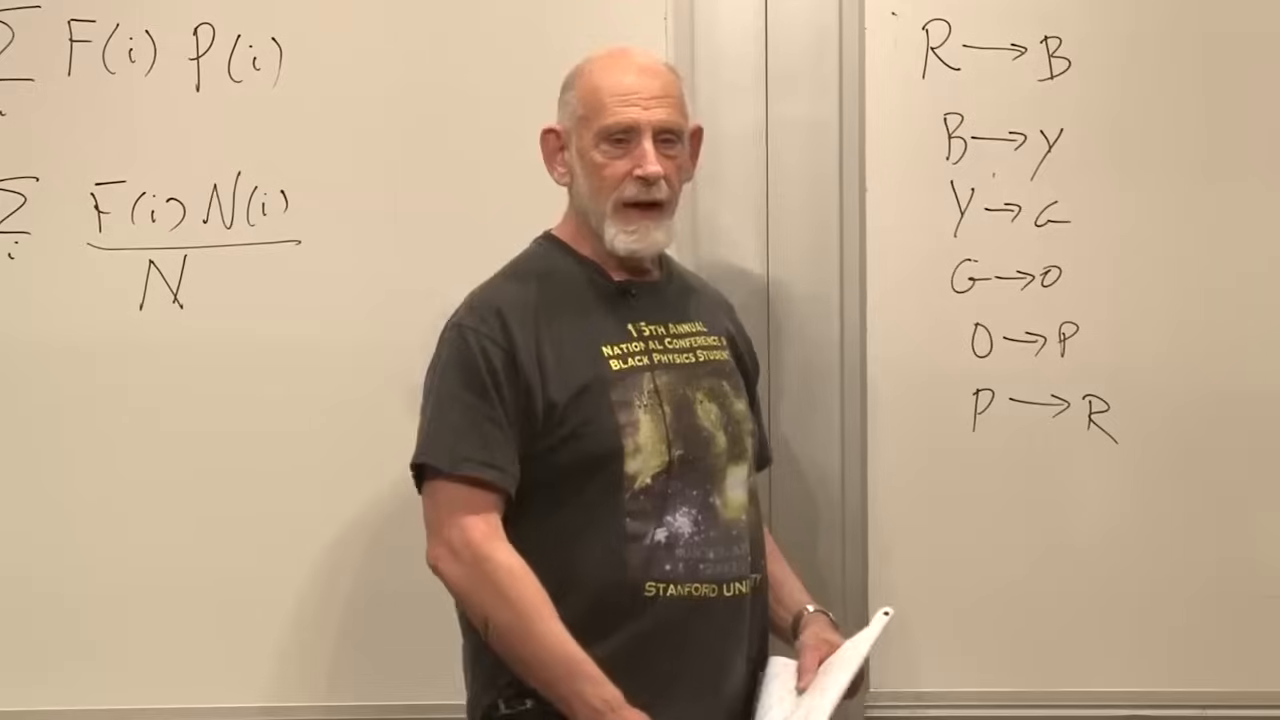
\includegraphics[width=0.92\textwidth]{lecture_01_figure_02.png}
\caption{기댓값 공식은 왼쪽 칠판에 그대로 두고, 결정론적 색상 갱신 규칙 여섯 가지는 오른쪽에 나열했다.}
\lectureframe{00:26:28}
\end{figure}

칠판에 나열된 규칙은 다음과 같이 방향이 있는 순환으로 나타내면 더 명확하다:
\begin{figure}[htbp]
\centering
\begin{tikzpicture}[
  >=Latex,
  state/.style={draw,circle,minimum size=8mm,inner sep=1pt}
]
\node[state] (R) at (90:2.2) {$R$};
\node[state] (B) at (30:2.2) {$B$};
\node[state] (Y) at (-30:2.2) {$Y$};
\node[state] (G) at (-90:2.2) {$G$};
\node[state] (O) at (-150:2.2) {$O$};
\node[state] (P) at (150:2.2) {$P$};
\draw[->] (R) -- (B);
\draw[->] (B) -- (Y);
\draw[->] (Y) -- (G);
\draw[->] (G) -- (O);
\draw[->] (O) -- (P);
\draw[->] (P) -- (R);
\end{tikzpicture}
\caption{여섯 상태로 이루어진 단일 궤도. 한 주기 동안 모든 상태를 한 번씩 방문한다.}
\label{fig:sm1-six-cycle}
\end{figure}

초기 상태를 모르고 시각도 알 수 없는 때에 스냅숏을 찍는다고 하자. 각 단계의 지속 시간이 같으므로 계는 각 색깔 상태에 주기의 6분의 1씩 머문다.
\begin{equation}
 p(R)=p(B)=p(Y)=p(G)=p(O)=p(P)=\frac16.
 \label{eq:sm1-uniform-cycle}
\end{equation}
이 등확률성은 물체의 모양에서 비롯되지 않는다. 각 상태에 머무는 시간이 같은 데서 나온다.

화살표 순서를 바꾸면 미시적 법칙은 달라지지만, 여전히 여섯 상태가 하나의 순환을 이룰 수 있다. 세부적인 순서는 바뀌어도 스냅숏 확률은 \(1/6\)로 유지된다. 각 상태가 주기마다 한 번씩 나타나기 때문이다. 따라서 이 예측에는 출발점이나 세부 순서가 필요하지 않다. 궤도의 구조와 갱신 단계마다 같은 시간이 든다는 사실만 있으면 된다.

\begin{classroomqa}
\classquestion{물체가 대칭이 아닌데도 모든 색깔에 확률 \(1/6\)를 부여하는 것은 어떤 의미에서 정당한가?}
\lecturerresponse{이 확률 배정은 기하학적 대칭성이 아니라 동역학에 근거한다. 여섯 단계 궤도에서 어느 위상에 있는지 모르는 상태로 스냅숏을 찍으면 동일한 시간 간격의 여섯 시간 구간을 표본으로 얻게 된다. 여기서 동등한 것은 물체의 면이 아니라 궤도상의 위치다. 각 상태에 머무는 시간이 서로 다르다면 확률도 서로 달라진다.
\lecturetimestamp{00:27:11--00:29:49}}
\end{classroomqa}

\section{분리된 순환과 보존량}

결정론적 법칙이 모든 상태를 하나의 궤도에 놓을 필요는 없다. 서로 연결되지 않은 두 순환을 생각해 보자.
\begin{equation}
 R\longrightarrow B\longrightarrow G\longrightarrow R,
 \qquad
 P\longrightarrow Y\longrightarrow O\longrightarrow P.
 \label{eq:sm1-two-cycles}
\end{equation}
계가 첫 번째 순환에 있다는 것을 안다면,
\begin{equation}
 \begin{aligned}
 p(R)=p(B)=p(G)&=\frac13,\\
 p(P)=p(Y)=p(O)&=0.
 \end{aligned}
\end{equation}
두 번째 순환에 있다는 것을 알면 이 확률 배정은 반대가 된다.

더 일반적인 경우에는 사전 가중치가 필요하다. 순환을 \(+1\)와 \(-1\)로 표시하고, 각각의 확률을 \(p_+\)와 \(p_-\)라 하자. 이때
\begin{equation}
 p_++p_-=1.
\end{equation}
그러면 다음과 같다.
\begin{align}
 p(R)=p(B)=p(G)&=\frac{p_+}{3},\\
 p(P)=p(Y)=p(O)&=\frac{p_-}{3}.
 \label{eq:sm1-sector-weights}
\end{align}
계수 \(1/3\)는 순환 안에서의 운동으로 정해진다. 반면 \(p_+\)와 \(p_-\)는 그렇지 않다. 이 값들은 다른 실험이나 초기 섹터를 선택하는 다른 계처럼 추가적인 지식에서 얻어야 한다.

표지 \(+1\)와 \(-1\)는 보존량을 정의한다. 계가 한 순환에서 시작하면 갱신 법칙은 그 계를 다른 순환으로 옮기지 않는다. 이 양을 에너지라고 부를 수도 있고, \emph{질크} 같은 임시 이름을 붙일 수도 있다. 이름은 부차적이다. 보존된다는 것은 동역학이 넘나들 수 없는 영역들로 상태공간이 나뉜다는 뜻이다.

순환마다 상태 수가 같을 필요는 없다. 네 상태 궤도와 두 상태 궤도도 두 개의 보존 섹터를 이룬다. 그러면 같은 시간 동안 표본을 취할 때 첫 번째 섹터 안에서는 \(1/4\), 두 번째 섹터 안에서는 \(1/2\)의 확률이 주어지며, 각 확률에는 해당 섹터의 사전 확률을 곱한다. 통계역학은 논리적으로 서로 다른 두 질문에 답해야 한다.
\begin{enumerate}
\item 보존 섹터가 주어졌을 때, 동역학은 그 안의 상태들에 시간을 어떻게 배분하는가?
\item 보존 섹터 자체에는 어떤 확률을 부여해야 하는가?
\end{enumerate}

\begin{classroomqa}
\audiencequestion{보존 섹터 하나 안의 모든 상태에 같은 확률을 부여한다고 가정하는 건가요?}
\lecturerresponse{여기서 제시한 이산 장난감 법칙에서는 그렇다. 각 상태가 같은 시간 간격 동안 지속되고 운동이 결정론적이기 때문이다. 불확실성은 궤도의 초기 위상에 있다. 밀리초 단위로 시간을 재는 검출기로는 마이크로초 단위 갱신을 분해할 수 없지만, 충분히 빠른 스냅숏이라면 포착된 상태를 알아낼 수 있다. 더 일반적인 계에서는 상태별로 머무는 시간이 다를 경우 이를 명시적으로 반영해야 한다.
\lecturetimestamp{00:36:16--00:37:17}}
\end{classroomqa}

\begin{classroomqa}
\audiencequestion{스냅숏을 두 번 찍었을 때 첫 번째 결과로 순환 하나를 알아냈다면, 두 번째 결과에서도 같은 순환이 나와야 하나요?}
\lecturerresponse{그렇다. 바로 그것이 보존의 뜻이다. 측정으로 보존량의 값을 알아내면, 이후 확률은 그 값을 조건으로 삼아 정할 수 있고 다른 섹터에 속한 상태의 확률은 0이 된다.
\lecturetimestamp{00:37:18--00:37:45}}
\end{classroomqa}

\subsection{두 계 사이에서 나뉘는 에너지}

이제 추상적인 표지 대신 에너지를 생각해 보자. 고립된 상자 하나는 닫힌계이므로 보존되는 에너지를 갖는다. 서로 상호작용하지 않는 고립된 상자 두 개에는 각각 따로 보존되는 에너지가 있다. 에너지가 이동할 수 있도록 두 상자를 좁은 통로로 연결하면 각 에너지는 변할 수 있지만 전체 에너지는 일정하게 유지된다.

\begin{figure}[htbp]
\centering
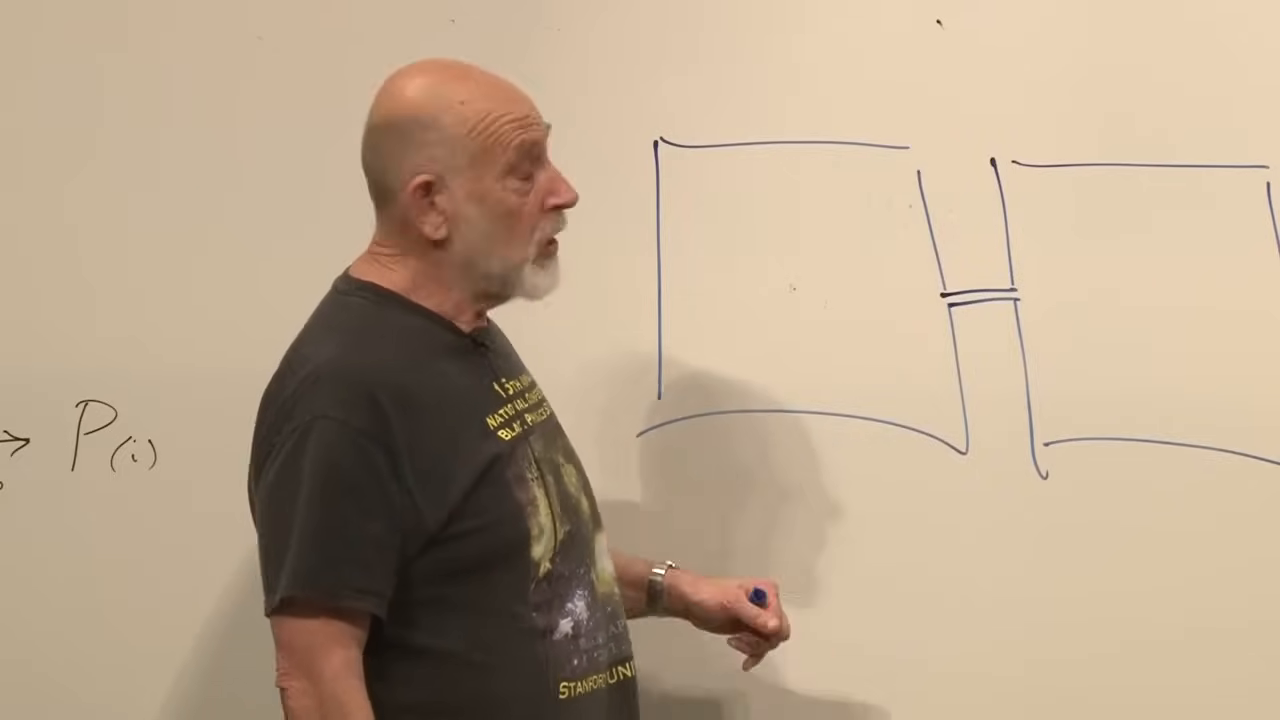
\includegraphics[width=0.92\textwidth]{lecture_01_figure_03.png}
\caption{에너지가 통과할 수 있는 좁은 통로로 연결된 두 부분계.}
\lectureframe{00:39:19}
\end{figure}

\begin{figure}[htbp]
\centering
\begin{tikzpicture}[>=Latex]
\draw[thick,rounded corners=4pt] (-4,1.8) rectangle (-0.7,-1.5);
\draw[thick,rounded corners=4pt] (0.7,1.5) rectangle (4,-1.8);
\draw[thick] (-0.7,0.45) -- (0.7,0.45);
\draw[thick] (-0.7,-0.35) -- (0.7,-0.35);
\draw[<->,very thick] (-0.45,0.05) -- (0.45,0.05);
\node at (-2.35,0.15) {subsystem \(1\)};
\node at (2.35,-0.15) {subsystem \(2\)};
\node[above] at (0,0.5) {energy exchange};
\end{tikzpicture}
\caption{연결을 열면 보존되는 것은 \(E_1+E_2\)뿐이다. 에너지의 분배는 확률 문제로 바뀐다.}
\label{fig:sm1-connected-systems}
\end{figure}

전체 에너지가 주어졌을 때, 부분계 \(1\)의 에너지가 \(E_1\)이고 부분계 \(2\)의 에너지가 나머지인 확률을 물을 수 있다. 같은 크기의 상자라면 평균 에너지도 같아야 하지만, 평균만으로 분포 전체를 알 수는 없다. 따라서 부분계의 확률을 정하는 한 가지 방법은 보존법칙이 필요한 정보를 제공하는 더 큰 닫힌계 안에 그 부분계를 두는 것이다. 이 구성은 통계역학에서 거듭 등장한다.

\section{좋은 법칙, 나쁜 법칙, 그리고 마이너스 제1법칙}

모든 결정론적 갱신 규칙이 근본 법칙으로 허용되는 것은 아니다. 다음 사상을 보자.
\begin{equation}
 \begin{aligned}
 R&\mapsto R,& B&\mapsto R,& Y&\mapsto R,\\
 G&\mapsto R,& O&\mapsto R,& P&\mapsto R.
 \end{aligned}
 \label{eq:sm1-all-to-red}
\end{equation}
이 사상은 미래를 완벽하게 예측한다. 한 단계 뒤에는 상태가 빨간색이 된다. 하지만 반대 방향으로는 문제가 있다. 계가 빨간색이 된 뒤에는 파란색, 노란색, 초록색, 주황색, 보라색 또는 빨간색 자체 중 어느 상태에서 왔는지 알 수 없다.

\begin{figure}[htbp]
\centering
\begin{tikzpicture}[
  >=Latex,
  state/.style={draw,circle,minimum size=8mm,inner sep=1pt}
]
\node[state,fill=red!12] (R) at (0,0) {$R$};
\node[state] (B) at (-3,1.6) {$B$};
\node[state] (Y) at (-3,0) {$Y$};
\node[state] (G) at (-3,-1.6) {$G$};
\node[state] (O) at (3,1.6) {$O$};
\node[state] (P) at (3,-1.6) {$P$};
\draw[->] (B) -- (R);
\draw[->] (Y) -- (R);
\draw[->] (G) -- (R);
\draw[->] (O) -- (R);
\draw[->] (P) -- (R);
\draw[->,loop above] (R) to (R);
\end{tikzpicture}
\caption{다대일 법칙은 다음 상태를 예측하지만, 가능한 과거 상태들 사이의 구별을 지워 버린다.}
\label{fig:sm1-bad-law}
\end{figure}

반면 닫힌 순환은 기록을 보존한다. 경과 시간을 알고 있으면 수천 주기가 지난 뒤에도 상태를 미래나 과거 방향으로 변화시킬 수 있다. 이 법칙은 초기 조건 사이의 차이를 보존한다. Susskind는 이 요구를 \emph{물리학의 마이너스 제1법칙}이라고 부른다. 정보는 근본적으로 사라지지 않는다.

유한한 이산 상태공간에서는 그림으로 나타낸 기준이 간단하다.
\begin{quote}
좋은 법칙에서는 모든 상태에 나가는 화살표가 정확히 하나 있고, 들어오는 화살표도 정확히 하나 있다.
\end{quote}
나가는 화살표는 미래를 정하고, 들어오는 화살표는 과거를 복원한다. 수학적으로 갱신은 상태들의 순열이다.

\subsection{마찰은 겉보기 반례일 뿐}

연속적인 계에 해당하는 정리는 리우빌 정리다. 마찰은 이 정리에 모순되는 듯 보인다. 지우개를 책상 위에서 밀면 어디에서 시작하든 결국 멈춘다. 저항력을 나타내는 개략적인 방정식은 다음과 같다.
\begin{equation}
 m\ddot x=-\gamma\dot x,
 \qquad \gamma>0.
 \label{eq:sm1-drag}
\end{equation}
속도는 지수적으로 감소한다. 봉인된 방에 있는 모든 입자에 적용되는 근본 법칙이 이것뿐이라면, 모든 운동이 사라지고 온도가 0까지 떨어지며 많은 초기 상태가 하나의 최종 상태로 합쳐질 것이다. 에너지 보존은 깨지고, 정보는 사라지며, 무질서도 감소할 것이다. 이는 모든 상태가 빨간색으로 가는 연속계 버전이다.

실제 마찰은 이런 식으로 작용하지 않는다. 지우개는 책상과 지우개 자체, 그리고 주변 환경을 가열한다. 미시적인 위치와 운동량에는 눈에 보이는 운동에서 사라진 구분이 기록된다. 마찰은 관측하지 않은 자유도를 생략한 뒤 부분계에 적용하는 유효 방정식이다. 완전한 닫힌계에 적용되는 근본적인 소산 법칙은 아니다.

\begin{classroomqa}
\classquestion{미분방정식
\(m\ddot x=-\gamma\dot x\)은 무엇을 나타내며, 왜 닫힌계의 근본 법칙이 아닌가요?}
\lecturerresponse{이 방정식은 점성 저항력을 나타낸다. 방정식만 따로 보면 모든 속도를 0으로 이끌며, 이는 초기 온도와 관계없이 기체를 0까지 냉각시킨다. 실제 닫힌계를 기술할 때는 사라진 역학적 에너지와 정보가 미시적 자유도로 옮겨간다. 저항력 방정식은 그런 변수들을 생략한 뒤에만 유효하다.
\lecturetimestamp{00:44:40--00:48:56}}
\end{classroomqa}

\section{점유 상태와 첫 번째 엔트로피}

정보 보존에는 이에 상응하는 확률론적 진술이 있다. 같은 확률을 부여받는 상태가 \(M\)개이고, 전체 상태는 \(N\)개라고 하자.
\begin{equation}
 p_i=
 \begin{cases}
 1/M, & i\text{ in the occupied set},\\
 0, & i\text{ outside it}.
 \end{cases}
 \label{eq:sm1-uniform-occupied}
\end{equation}
정보를 보존하는 갱신은 점유된 상태들을 재배열할 수는 있지만 하나로 합칠 수는 없다. 이후 어느 시점에도 확률이 \(1/M\)인 상태는 \(M\)개 그대로다. 반면 잘못된 사상 \eqref{eq:sm1-all-to-red}은 점유된 여러 상태를 하나로 합칠 수 있다.

수 \(M\)는 무지를 나타낸다. \(M=N\)이면 모든 상태가 가능하고 무지가 최대다. \(M=1\)이면 미시적 상태를 정확히 알고 있다. 따라서 엔트로피를 처음 정의하면 다음과 같다.
\begin{equation}
 S=\log M.
 \label{eq:sm1-entropy-logm}
\end{equation}
그러면 다음을 얻는다.
\begin{equation}
 S_{\max}=\log N,
 \qquad
 S_{\min}=0.
\end{equation}
상태공간이 무한하면 유한한 상한이 없을 수도 있다.

이 전개에서는 온도보다 먼저 엔트로피가 등장하며, 에너지 보존을 정식으로 서술하기도 전에 나온다. 그런 의미에서 엔트로피가 더 원초적이다. 그러나 엔트로피는 역학계 자체만의 성질은 아니다. 엔트로피는 계와 알려진 바를 나타내는 확률분포에 함께 의존한다. 서로 다른 정보를 가진 관측자는 같은 역학계에 서로 다른 엔트로피를 부여할 수 있다.

정확한 미시적 시간발전에서는 점유된 상태들이 재배열될 뿐이므로 이 세분된 엔트로피는 보존된다. 실제로는 시간 측정을 놓치고, 상관관계를 버리며, 엄청나게 많은 변수를 추적하지 못한다. 그러면 확률분포가 더 많은 대안에 걸쳐 퍼지고, 거친 기술에 부여되는 엔트로피가 증가한다. 우리가 쓸 수 있는 기술에서 정보가 사라지더라도 방정식 자체가 정보를 파괴할 필요는 없다.

\begin{classroomqa}
\classquestion{상태가 \(N\)개인 유한한 계에서 가능한 최대 엔트로피는 얼마인가요?}
\lecturerresponse{그 값은 \(\log N\)이며, \(N\)개 상태 모두가 같은 확률일 때 달성된다. 최소 엔트로피는 0이며, 상태 하나의 확률이 1일 때 달성된다. 따라서 엔트로피는 이용 가능한 상태공간뿐 아니라 지식의 상태도 측정한다.
\lecturetimestamp{00:56:46--00:58:19}}
\end{classroomqa}

\section{연속 위상공간에서의 리우빌 흐름}

위치와 운동량이 연속적으로 변하는 입자에서 미시적 상태는 위상공간의 한 점이다. 좌표를 \(q_a\), 그 켤레 운동량을 \(p_a\)라고 쓰자. 입자가 많으면 축도 엄청나게 많다. \(q\)축 하나와 \(p\)축 하나로 그린 2차원 그림은 실제를 대신한 모형일 뿐이다. 각 좌표에 대응하는 운동량이 있으므로 위상공간의 차원은 짝수다.

우리의 지식을 영역 \(\Omega_0\)로 나타낸다고 하자. 확률밀도는 그 영역 안에서 균일하고 바깥에서는 0이다. 예를 들어 모든 입자가 방 안에 있다는 사실을 알면 위치 좌표의 범위가 제한되고, 속도에 상한과 하한을 두면 운동량 좌표의 범위가 제한된다.

해밀토니안 시간 발전은 위상 공간의 각 점을 궤적을 따라 이동시킨다. 서로 가까운 점은 가까운 점으로 이동하고, 점유된 영역은 비압축성 유체의 한 덩어리처럼 흐른다:
\begin{figure}[htbp]
\centering
\begin{tikzpicture}[>=Latex,scale=0.95]
\draw[->] (-4.2,0) -- (4.3,0) node[right] {$q$};
\draw[->] (-3.7,-2.2) -- (-3.7,2.4) node[above] {$p$};
\draw[fill=blue!12,thick]
  (-3.0,-0.5) .. controls (-2.7,1.0) and (-1.3,1.2) .. (-0.9,0.1)
  .. controls (-0.6,-1.0) and (-2.2,-1.4) .. cycle;
\node at (-1.9,0.0) {$\Omega_0$};
\draw[->,very thick] (-0.3,0.2) -- (0.8,0.2);
\draw[fill=orange!15,thick]
  (1.2,-1.1) .. controls (1.5,0.3) and (2.3,1.8) .. (3.2,1.1)
  .. controls (3.6,0.7) and (2.8,-0.4) .. (2.5,-1.5)
  .. controls (2.1,-1.8) and (1.5,-1.6) .. cycle;
\node at (2.35,0.1) {$\Omega_t$};
\end{tikzpicture}
\caption{해밀토니안 흐름은 점유된 위상 공간 영역을 늘이고 비틀 수 있지만, 그 부피는 보존한다.}
\label{fig:sm1-liouville-flow}
\end{figure}

리우빌 정리는 다음과 같이 말한다.
\begin{equation}
 \operatorname{Vol}(\Omega_t)
 =
 \operatorname{Vol}(\Omega_0).
 \label{eq:sm1-liouville-volume}
\end{equation}
초기 밀도가 \(\Omega_0\)에서 균일하면, 시간에 따라 이동한 밀도는 \(\Omega_t\)에서 균일하다. 이는 점유된 이산 상태의 수와 가중치를 보존하는 것에 해당하는 연속적 명제다.

이 정리는 마찰 문제를 기하학적으로도 해결한다. 지우개의 눈에 보이는 운동량만 보면 가능한 상태의 분포가 \(p=0\) 쪽으로 모이는 듯하다. 하지만 전체 위상공간에서는 그 분포가 지우개와 책상 분자들의 위치와 운동량에 걸쳐 퍼진다. 전체 고차원 부피가 일정한 채로 투영은 수축할 수 있다.

\begin{classroomqa}
\classquestion{눈에 보이는 모든 궤적이 정지 상태로 다가간다면 점유된 위상공간 영역은 축 \(p=0\) 위의 한 점으로 붕괴한 건가요?}
\lecturerresponse{줄어든 투영에서만 그렇다. 전체 계에는 책상과 지우개, 주변 환경의 미시적 변수가 들어 있다. 눈에 보이는 운동량 범위가 좁아지는 동안 분포는 숨겨진 방향들로 퍼진다. 리우빌 정리는 불완전한 거시적 변수 집합이 아니라 완전한 닫힌 위상공간에 적용된다.
\lecturetimestamp{01:04:37--01:06:29}}
\end{classroomqa}

\section{마이너스 제1법칙에서 제1법칙까지}

\subsection{영 법칙을 잠시 살펴보기}

첫째 법칙을 진술하기 전에 영 법칙을 먼저 소개하는 것이 유용하다. 아직 열평형을 정의하지 않았으므로, 지금은 이 법칙을 구조에 관한 명제로만 제시한다:
\begin{quote}
계 \(A\)이 계 \(B\)와 열평형에 있고, 계 \(B\)가 계 \(C\)와 열평형에 있다면, 계 \(A\)는 계 \(C\)와 열평형에 있다.
\end{quote}
이 추이성이 나중에 온도의 개념을 가능하게 한다. 지금은 이 점을 잠시 미뤄 둔다.

\subsection{에너지 보존}

닫힌계에 대한 제1법칙은 간단히 다음과 같다.
\begin{equation}
 \frac{dE}{dt}=0.
 \label{eq:sm1-first-law}
\end{equation}
이 간결한 식은 그 힘을 감추고 있다. 에너지는 보존량이며, 에너지라는 말은 뒤에서 더 풍부한 열역학적 의미를 갖게 된다.

닫힌계가 두 부분으로 이루어져 있고 각 부분의 에너지가 가산적이라면,
\begin{equation}
 E=E_1+E_2,
\end{equation}
다음과 같이 쓸 수 있다.
\begin{equation}
 \frac{dE_1}{dt}+\frac{dE_2}{dt}=0,
 \qquad\text{or}\qquad
 \frac{dE_1}{dt}=-\frac{dE_2}{dt}.
 \label{eq:sm1-energy-exchange}
\end{equation}
두 번째 식은 에너지 교환을 명시적으로 드러낸다. 한 부분계가 잃은 에너지는 다른 부분계가 얻는다.

가산성 가정에는 주의가 필요하다. 중력으로 상호작용하는 두 입자에는 각각의 운동에너지가 있지만, 두 입자의 상호작용은 쌍에 속하는 퍼텐셜 에너지를 더한다. 두 물체의 에너지를 합한 값으로 정확히 쓸 수는 없어도 전체 에너지는 보존된다.

열역학에서는 가산적인 근사가 매우 잘 성립하는 경우가 많다. 거시적인 에너지는 부피에 비례하는 반면, 가까이 맞닿은 큰 부분들 사이의 짧은 거리 상호작용 에너지는 주로 접촉 면적에 비례하기 때문이다. 큰 탁자를 여러 블록으로 나누어 보자. 각 블록의 내부 에너지는 부피 효과인 반면, 이웃 블록 사이의 결합은 표면 효과다. 블록이 크면 후자는 상대적으로 작다. 식 \eqref{eq:sm1-first-law}은 닫힌계 전체에 대해 정확하다. 부분계에 적용하는 식 \eqref{eq:sm1-energy-exchange}은 상호작용 에너지가 무시할 만하다고 가정한다.

\begin{classroomqa}
\audiencequestion{정규화 조건 \(\sum_i p_i=1\)도 나열된 결과들이 서로 배타적이라고 가정하나요?}
\lecturerresponse{그렇다. 상태 표지는 대안들이 서로 겹치지 않도록 정의된다. 주사위가 노란색 상태라면 동시에 빨간색 상태일 수 없다. 일상적인 표현에서는 색을 섞어 말할 수 있지만, 확률 계산에 사용하는 상태 분할은 서로 배타적인 대안들로 이루어져야 한다.
\lecturetimestamp{01:12:14--01:12:55}}
\end{classroomqa}

\section{엔트로피로 돌아가기}

이제 강의는 앞서 다루다 만 주제로 명시적으로 돌아간다. 감각적으로 익숙한 온도는 유도되는 물리량이다. 온도를 명확히 정의하려면 엔트로피와 에너지가 먼저 정립되어야 한다.

\subsection{일반적인 확률분포}

특수한 정의 \(S=\log M\)는 \(M\)개 상태가 같은 확률을 갖고 나머지 상태의 확률은 모두 0일 때 적용된다. 일반적인 분포는 직사각형 모양일 필요가 없다. 상태 표지에 따라 가중치가 매끄럽게 변할 수도 있고 불규칙하게 변할 수도 있다.

\begin{figure}[htbp]
\centering
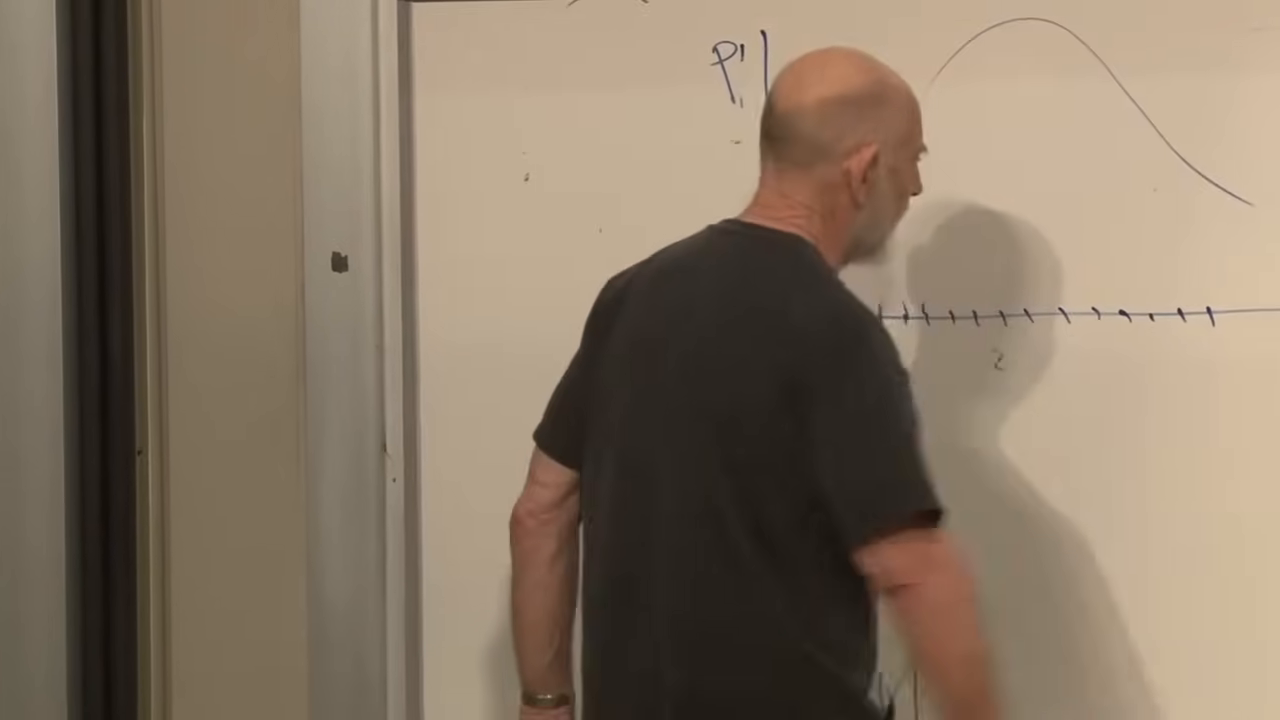
\includegraphics[width=0.92\textwidth]{lecture_01_figure_05.png}
\caption{이산적인 상태 표지 위에 그린 확률분포. 엔트로피를 구하는 데 필요한 특징은 정확한 곡선이 아니라 분포의 퍼짐이다.}
\lectureframe{01:14:40}
\end{figure}

\begin{figure}[htbp]
\centering
\resizebox{\linewidth}{!}{%
\begin{tikzpicture}[>=Latex,scale=0.93]
\draw[->] (-4.2,0) -- (4.4,0) node[right] {state label \(i\)};
\draw[->] (-4,0) -- (-4,3.2) node[above] {$p_i$};
\foreach \x in {-3.6,-3.1,...,3.6}
  \draw (\x,0.08) -- (\x,-0.08);
\draw[very thick]
  plot[smooth] coordinates {
  (-3.7,0.12) (-3.0,0.28) (-2.3,0.72) (-1.6,1.45)
  (-0.9,2.25) (-0.2,2.65) (0.5,2.28) (1.2,1.55)
  (1.9,0.88) (2.7,0.38) (3.5,0.14)};
\draw (-1.8,-0.18) -- (-1.8,-0.5);
\draw (1.8,-0.18) -- (1.8,-0.5);
\draw[<->] (-1.8,-0.46) -- (1.8,-0.46);
\node at (0,-0.82) {effective spread};
\end{tikzpicture}
}
\caption{좁은 분포는 넓은 분포보다 불확실성이 작다. 엔트로피는 분포 전체를 측정해야 한다.}
\label{fig:sm1-probability-spread}
\end{figure}

일반적인 정의는 다음과 같다.
\begin{equation}
 S=-\sum_i p_i\log p_i.
 \label{eq:sm1-shannon-entropy}
\end{equation}
\eqref{eq:sm1-expectation}를 사용하면 다음과 같이 쓸 수 있다.
\begin{equation}
 S=-\langle\log p\rangle.
\end{equation}
\(\log p_i<0\)라는 점을 고려하면 \(0<p_i<1\)일 때 음의 부호가 필요하다.

\subsection{균일분포 결과 되찾기}

일반식이 첫 번째 정의를 재현하는지 확인해야 한다.
비점유 상태에서는 \(p_i=0\)인 반면, \(\log p_i\)는 발산한다. 두 항의 곱은 극한에서 다음과 같이 잘 정의된 값을 갖는다.
\begin{equation}
 \lim_{p\to0^+}p\log p=0.
 \label{eq:sm1-plogp-limit}
\end{equation}
따라서 확률이 0인 상태는 기여하지 않는다.

\begin{classroomqa}
\audiencequestion{\(p_i=0\)이면 이 항은 정말 사라지나요? 영의 로그는 음의 무한대입니다.}
\lecturerresponse{이 항은 \(\lim_{p\to0^+}p\log p\)로 정의되며, 그 값은 영입니다. 인자 \(p\)는 로그가 발산하는 것보다 더 빠르게 영에 가까워집니다. 따라서 확률이 임의로 작아지는 상태들은 임의로 작은 기여를 하고, 정확히 불가능한 상태는 전혀 기여하지 않습니다.
\lecturetimestamp{01:18:27--01:19:46}}
\end{classroomqa}

점유된 \(M\)개의 상태 각각에 대해 \(p_i=1/M\)이다. 따라서
\begin{align}
 S
 &=-\sum_{\mathrm{occupied}\ i}
 \frac1M\log\!\left(\frac1M\right)\\
 &=-M\frac1M\log\!\left(\frac1M\right)\\
 &=-\log\!\left(\frac1M\right)
 =\log M.
 \label{eq:sm1-entropy-check}
\end{align}
일반식은 특수한 경우의 식과 정확히 일치한다. 분포가 넓게 퍼져 있으면 더 많은 대안에 상당한 확률이 부여되므로 엔트로피가 더 크고, 분포가 좁으면 엔트로피가 더 작다.

\begin{figure}[htbp]
\centering
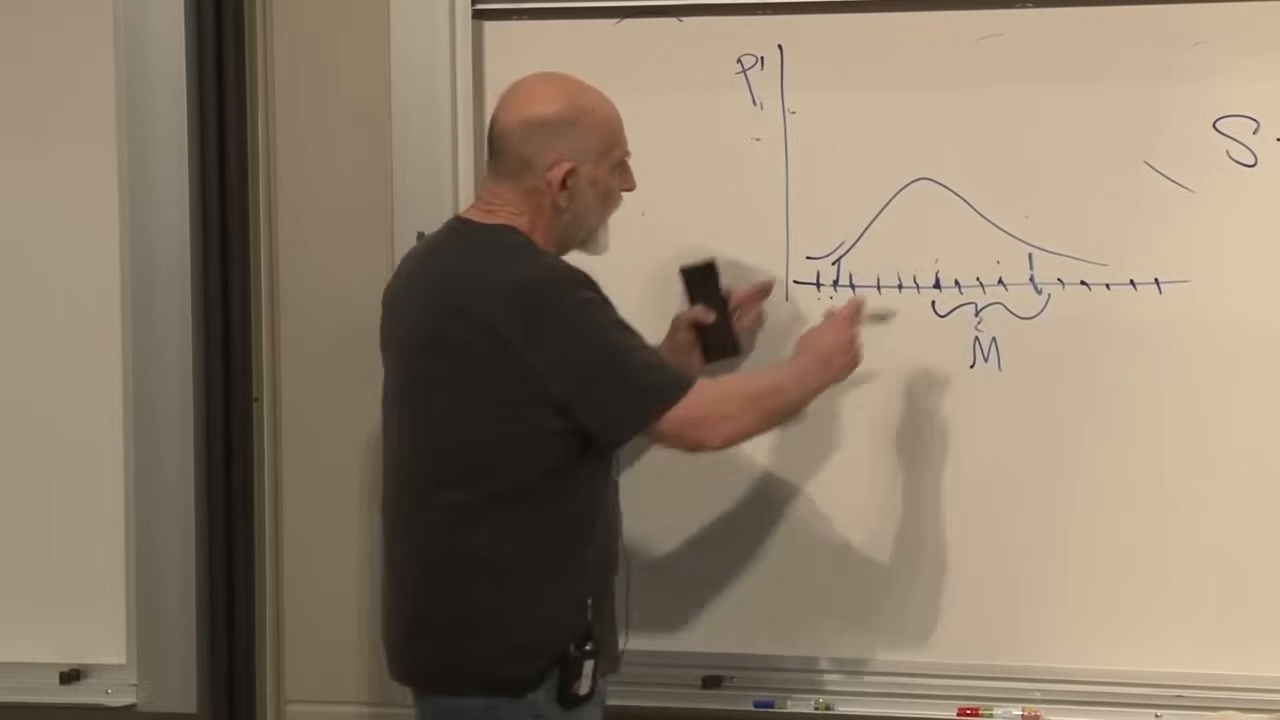
\includegraphics[width=0.92\textwidth]{lecture_01_figure_06.png}
\caption{표시된 폭 \(M\)은 유의미한 확률들의 분포 폭과 엔트로피 사이의 관계를 강조한다.}
\lectureframe{01:16:42}
\end{figure}

엔트로피는 상태 공간 위의 확률분포에 속한다. 한 미시상태의 에너지나 운동량 같은 단순한 관측량이 아니다. 정확한 상태는 그 상태에 집중된 확률분포로 나타낼 수 있으며, 이 경우 엔트로피는 0이다. 그러나 지식의 상태가 달라지면 엔트로피도 달라진다.

\section{동전, 비트, 명시적 계수}

동전의 개수를 \(n\)라고 하자. 미시적 배열의 수는
\begin{equation}
 N=2^n.
 \label{eq:sm1-coin-state-count}
\end{equation}
동전에 대해 아무것도 모른다면 \(2^n\)개의 배열이 모두 같은 확률을 가지며,
\begin{equation}
 S_{\max}=\log(2^n)=n\log2.
 \label{eq:sm1-coin-max-entropy}
\end{equation}
엔트로피는 서로 독립인 동전의 수에 비례해 가산적이다.

밑이 \(2\)인 로그를 사용하면, 두 상태를 가지는 계에 대해 아무것도 모를 때 엔트로피는 1비트다. 자연로그를 사용하면 엔트로피는 \(\log2\)이다. 단위는 관례에 따라 정해지지만, 순서 관계와 가산성은 변하지 않는다.

반대로 동전 하나하나의 상태를 모두 알고 있다면, 정확히 하나의 배열만 확률 1을 갖는다.
\begin{equation}
 S=0.
\end{equation}
아는 것이 많을수록 엔트로피는 작아진다.

이제 \(n\)개의 동전 가운데 정확히 하나만 뒷면이고 나머지는 모두 앞면이며, 뒷면이 어느 위치에 있는지는 모른다고 하자. 뒷면의 위치가 달라지는 \(n\)개의 배열이 같은 확률을 가지므로,
\begin{equation}
 S=\log n.
 \label{eq:sm1-one-tail-entropy}
\end{equation}
이는 일반적으로 \(\log2\)의 정수배가 아니다. 비트는 편리한 단위이지, 모든 엔트로피가 정수 비트 단위로만 나타난다는 뜻은 아니다.

\begin{classroomqa}
\audiencequestion{\(\log2\)는 동전마다 가능한 상태가 두 가지라서 나오는 것뿐인가? 원소의 상태가 세 가지라면 \(\log3\)이 되는가?}
\lecturerresponse{그렇다. \(k\)개의 가능한 상태를 가진 원소의 상태를 균일하게 모르는 경우 그 원소의 기여분은 \(\log k\)이다. 컴퓨터에서 이진 스위치가 특히 편리한 이유는 물리적 스위치가 두 안정 상태를 자연스럽게 구현하고, 2가 자명하지 않은 가장 작은 정수이기 때문이다.
\lecturetimestamp{01:29:55--01:30:48}}
\end{classroomqa}

\begin{classroomqa}
\audiencequestion{로그의 밑은 무엇인가?}
\lecturerresponse{이 물리학 공식에서 \(\log\)는 자연로그를 뜻한다. 정보 이론에서는 흔히 밑이 \(2\)인 로그를 사용해 엔트로피를 비트 단위로 직접 나타낸다. 밑을 바꾸면 모든 엔트로피에 동일한 변환 계수가 곱해질 뿐, 물리적 결론은 달라지지 않는다.
\lecturetimestamp{01:30:49--01:32:06}}
\end{classroomqa}

\section{연속 위상공간의 엔트로피}

고전 위상공간 \(\Gamma\)으로 돌아가자. 확률밀도가 부피 \(V_\Gamma\)인 영역에서 균일하고 바깥에서는 0이라면, 확률이 같은 \(M\)개의 상태를 세는 것에 해당하는 식은 다음과 같다.
\begin{equation}
 S=\log\!\left(\frac{V_\Gamma}{V_0}\right).
 \label{eq:sm1-continuous-uniform}
\end{equation}
여기서 \(V_\Gamma\)는 좌표와 운동량으로 이루어진 고차원 전체 공간의 부피이지, 보통의 공간 부피가 아니다. 고정된 부피 \(V_0\)는 로그의 진수를 무차원으로 만드는 기준 위상공간 셀이다. \(V_0=1\)로 놓으면 칠판에서 사용한 약식 표기 \(S=\log V_\Gamma\)을 얻는다.

일반적인 확률밀도 \(P(q,p)\)의 경우, 이산합은 위상공간 적분으로 바뀐다. 정규화 조건은
\begin{equation}
 \int_\Gamma d\Gamma\,P(q,p)=1,
 \label{eq:sm1-continuous-normalization}
\end{equation}
이며 엔트로피는
\begin{equation}
 S=-\int_\Gamma d\Gamma\,
 P(q,p)\log\!\bigl[P(q,p)V_0\bigr].
 \label{eq:sm1-continuous-entropy}
\end{equation}
이다. 밀도는 위상공간 셀당 확률이다. 개념적으로 \eqref{eq:sm1-continuous-entropy}는 여전히 확률분포가 얼마나 넓게 퍼져 있는지를 나타낸다. 균일한 덩어리 분포의 경우에는 점유 부피를 기준 셀 단위로 나타낸 값의 로그가 된다. 이 고정된 셀을 바꾸면 모든 연속 엔트로피가 같은 가산 상수만큼 이동하므로 엔트로피 차이는 변하지 않는다.

\begin{classroomqa}
\audiencequestion{좌표 기호가 \(x\)에서 \(q\)로 바뀐 이유는 무엇인가?}
\lecturerresponse{물리적 변화는 없다. 고전역학에서는 좌표에 \(x\) 또는 \(q\)를, 켤레 운동량에 \(p\)를 흔히 사용한다. 표기법을 바꾼 것은 단순한 실수였으며 위상공간 구성은 동일하다.
\lecturetimestamp{01:37:10--01:37:39}}
\end{classroomqa}

온도와 볼츠만 분포는 의도적으로 뒤로 미루었다. 다음 과제는 열평형을 정의한 뒤 그에 해당하는 확률분포를 찾는 것이다.

\section{상관관계, 가산성, 정보에 관한 질문}

\subsection{상관관계란 한 측정이 다른 분포를 바꾼다는 뜻이다}

서로 독립인 동전에 대해 아무것도 모른다면 모든 배열에 같은 확률을 부여한다. 이때 동전 하나를 측정해도 다른 동전에 관해서는 아무것도 알 수 없다. 다른 동전들의 분포는 변하지 않는다.

뒷면이 하나인 앙상블은 다르다. 측정한 동전이 뒷면이면 나머지 동전은 모두 확실히 앞면이다. 측정한 동전이 앞면이면 유일한 뒷면은 나머지 \(n-1\)개의 동전 가운데 있어야 하므로, 남은 각 위치에 대한 조건부 확률은
\begin{equation}
\begin{aligned}
 p(&\text{tail at a specified remaining position}\\
   &\mid\text{measured head})=\frac{1}{n-1}.
\end{aligned}
 \label{eq:sm1-conditional-tail}
\end{equation}
이다. 이것이 상관관계다. 한 변수에 대해 알게 되면 다른 변수에 부여하는 확률분포가 달라진다.

\begin{classroomqa}
\audiencequestion{엔트로피 예시에서 동전들의 독립성을 가정했는가?}
\lecturerresponse{완전히 모르는 상태를 \(2^n\)개의 모든 배열에 같은 확률을 부여하는 것으로 나타낸 경우에만 그렇다. 이 경우 동전 하나를 측정해도 나머지 동전들의 분포는 달라지지 않는다. 뒷면이 하나인 예시는 명시적으로 상관되어 있다. 측정하면 다른 곳에서 가능한 상태에 대한 지식이 갱신된다. 주어진 정보에 따라 사용할 확률분포가 정해진다.
\lecturetimestamp{01:38:43--01:41:58}}
\end{classroomqa}

분리된 궤도 예시도 논리 구조가 같다. 보존되는 \(+1\) 또는 \(-1\) 라벨을 측정하면 이후 모든 상태는 하나의 섹터로 제한된다. 보존량에 관한 정보로 조건을 걸면 허용되는 분포가 달라진다.

상관관계가 없는 계들의 엔트로피는 가산적이다. 만약
\begin{equation}
 p_{ij}=p_i^{(A)}p_j^{(B)},
\end{equation}
이라면
\begin{align}
 S_{AB}
 &=-\sum_{i,j}p_i^{(A)}p_j^{(B)}
 \log\!\left[p_i^{(A)}p_j^{(B)}\right]\\
 &=S_A+S_B.
 \label{eq:sm1-entropy-additivity}
\end{align}
이다. 상관관계가 있으면 이 인수분해가 성립하지 않으며 두 계의 독립적인 불확실성은 줄어든다.

연습 삼아, 위 상태일 때 각 이웃 변수가 아래 상태일 확률이 사분의 삼이 되는 이진 변수들의 열을 생각해 보자. 한 위치를 측정하면 인접한 위치에 대해 아는 것이 곧바로 달라진다. 이 분포에는 상관관계가 있으므로, 상관관계를 고려하지 않고 각 위치 하나씩의 엔트로피를 더해서는 전체 엔트로피를 구할 수 없다.

\subsection{볼츠만, 섀넌, 양자 불확정성}

\begin{classroomqa}
\audiencequestion{열역학에서 더 오래전부터 쓰인 엔트로피는 섀넌의 정보 이론적 엔트로피와 어떤 관계인가?}
\lecturerresponse{두 경우에 같은 함수꼴이 나타난다.
\(-\sum_i p_i\log p_i\)섀넌은 흔히 밑이 \(2\)인 로그를 사용했고, 물리학자들은 대개 자연로그를 사용한다. 엔트로피를 열역학적 단위로 나타낼 때는 볼츠만 상수를 다시 곱한다. 수학적 차이는 고정된 변환 계수뿐이지만, 확률을 정하는 물리적 질문은 서로 크게 다를 수 있다.
\lecturetimestamp{01:44:05--01:46:06}}
\end{classroomqa}

미시상태들의 확률이 모두 같을 때 열역학 공식은 흔히 다음과 같이 쓴다.
\begin{equation}
 S_{\mathrm{thermo}}=k_{\mathrm B}\log W,
 \label{eq:sm1-boltzmann-formula}
\end{equation}
여기서 \(W\)는 접근 가능한 미시상태의 수다. \(k_{\mathrm B}=1\)인 단위계에서는 이 식이 정확히 \(S=\log W\)이다. 볼츠만 상수는 온도 단위와 에너지 단위 사이를 변환하며, 온도의 자연스러운 미시적 척도는 에너지다.

\begin{classroomqa}
\audiencequestion{이 엔트로피는 하이젠베르크의 불확정성 원리를 다른 방식으로 표현한 것인가?}
\lecturerresponse{아니다. 여기서 다루는 엔트로피는 가능한 상태들에 대한 확률분포의 불확실성을 측정한다. 양자역학의 언어로는 혼합 상태의 불확실성이지, 순수 상태에서도 남을 수 있는 본질적인 측정 불확실성이 아니다. 두 개념을 구별해야 한다.
\lecturetimestamp{01:46:07--01:47:31}}
\end{classroomqa}

\section{확립된 내용}

출발점은 법칙의 무작위성이 아니었다. 초기 상태에 대한 지식이 불완전하면 결정론적 동역학만으로도 이미 확률이 생긴다. 하나의 궤도에서는 각 상태에 머무는 시간으로 확률 가중치가 정해지고, 서로 분리된 궤도에서는 보존량이 드러나며 각 섹터에 사전 가중치를 부여해야 한다. 허용되는 미시 법칙은 구별되는 상태들을 보존한다. 유한 상태공간에서는 각 상태로 들어오는 화살표와 나가는 화살표가 각각 하나씩 있다는 뜻이며, 연속역학에서는 이를 리우빌 정리로 나타낸다.

이 구조에서 먼저 다음 식이 나온다.
\begin{equation}
 S=\log M
\end{equation}
확률이 같은 점유 상태 \(M\)개에 대해 성립하며, 이어서
\begin{equation}
 S=-\sum_i p_i\log p_i,
\end{equation}
가 나오고, 마지막으로 그 위상공간 적분식에 이른다. 엔트로피는 확률분포, 따라서 지식의 상태를 기록한다. 실용적인 거친 분해능의 기술이 정보를 놓치더라도 미시 법칙은 세분된 정보를 보존한다.

에너지 보존은 첫 번째 법칙을 주며, 부분계 에너지의 가산성에는 상호작용 에너지가 무시할 수 있어야 한다. 엔트로피의 가산성에도 이에 대응하는 조건이 있다. 부분계들의 확률은 서로 상관되어 있지 않아야 한다. 이 두 종류의 가산성을 바탕으로 다음 단계에서는 열평형, 온도, 볼츠만 분포를 통해 에너지와 확률을 연결한다.
\chapter{온도, 엔트로피와 에너지}

\lectureoverview{온도는 처음에 사람용 온도계 눈금을 미시적 에너지 단위로 환산하는 과정에서 등장한다. 이에 대응하여 열역학적 엔트로피를 무차원 통계적 엔트로피로 환산하고 나면, 평형은 하나의 매개변수로 표시되는 확률분포들의 족으로 기술된다. 미분 \(dE/dS\)로 온도를 정의할 수 있고, 열역학 제1법칙과 제2법칙은 온도 차이가 에너지 흐름의 방향을 정하는 이유를 보여 준다.}

\section{환산 인자와 사람의 단위}

물리학의 여러 상수는 환산 인자다. 빛의 속도는 거리를 시간으로 환산한다.
\begin{equation}
 t=\frac{x}{c}.
\end{equation}
거리와 시간을 서로 호환되는 단위로 측정한다면 \(c=1\)로 놓을 수 있다. 물리적 효과가 사라지는 것은 아니다. 두 종류의 측정값을 하나의 공통 척도로 나타냈을 뿐이다.

볼츠만 상수도 같은 성격을 지닌다. 사람의 척도에 맞춘 온도계로 읽은 온도를 에너지로 환산한다. \emph{사람의 척도에 맞춘}이라는 표현이 중요하다. 이런 단위는 거시적 기기로 구현하고 판독할 수 있기 때문에 선택한 것이지, 미시적 동역학이 특별히 선택한 단위이기 때문은 아니다.

섭씨 눈금은 표준 압력에서 물의 어는점과 끓는점 사이의 간격을 백 등분하여 정했다. 켈빈은 같은 크기의 눈금을 사용하지만 절대영도를 영점으로 삼는다. 다른 물질이나 다른 온도 간격, 또는 화씨 눈금을 선택해도 수치는 달라지지만 물리학은 달라지지 않는다.

\begin{classroomqa}
\audiencequestion{화씨 눈금도 이미 17세기에 만들어졌나요?}
\lecturerresponse{정확한 날짜는 여기서 중요하지 않다. 요점은 이런 눈금들이 모두 사람들이 만들고 측정할 수 있는 온도를 기준으로 고안되었다는 것이다. 눈금의 크기는 관례로 정한 것이지 미시적 기준에서 나온 것이 아니다.
\lecturetimestamp{00:01:34--00:01:50}}
\end{classroomqa}

이 눈금들이 만들어질 당시에는 열의 분자적 기원을 실험으로 밝힐 수 없었다. 거시적 온도계로 1도 변화를 관측할 수는 있었지만 분자 하나의 에너지는 측정할 수 없었다. 그러므로 온도가 근본적으로 에너지 척도라는 사실을 알기 전에 온도 단위를 정한 것은 자연스러운 일이었다.

\section{온도의 단위가 에너지인 이유}

희박 단원자 기체를 생각하자. 여기서 희박하다는 것은 현재 목적상 분자 사이의 상호작용 에너지를 무시할 수 있다는 뜻이다. 열평형에서는 등분배 법칙에 따라 각 이차 병진 자유도에 볼츠만 상수와 \(T_{\mathrm K}/2\)의 곱이 배정된다. 세 공간 차원에서는 \begin{equation}
 \left\langle E_{\mathrm{kin}}\right\rangle
 =\frac{3}{2}k_{\mathrm B}T_{\mathrm K}.
 \label{eq:sm2-equipartition-kelvin}
\end{equation} 인자 세는 \(x\), \(y\), \(z\) 방향의 운동을 센다. 절반이라는 계수는 이차 운동 에너지에서 비롯된다.

이 관계는 특정한 분자 종류에만 해당하지 않는다. 평형 상태의 헬륨과 산소 혼합물에서는 자유롭게 병진 운동하는 모든 입자의 질량중심 운동에너지가 평균적으로 같다. 무거운 입자가 더 느리게 움직이더라도 그렇다. 왜냐하면
\begin{equation}
 E_{\mathrm{kin}}=\frac{1}{2}mv^2,
\end{equation}
특징적인 에너지가 같으면 \(v\propto m^{-1/2}\)이기 때문이다.

같은 생각을 일부러 극단적인 사례에 적용해 볼 수도 있다. 볼링공을 유체에 담가 두고 계 전체가 평형에 이르게 하자. 볼링공의 브라운 병진 자유도도 분자의 자유도와 같은 에너지 척도로 결정된다. 볼링공의 속도는 질량이 엄청나게 크기 때문에 터무니없을 만큼 작지만, 온도는 속도가 아니라 에너지 척도를 비교한다.

실온에서 \(T_{\mathrm K}\)은 약 \(300\,\mathrm K\)인 반면, 미시적 자유도 하나의 에너지는 줄 단위로 보면 매우 작다. 따라서 환산 인자도 매우 작다.
\begin{equation}
 k_{\mathrm B}\simeq 1.38\times10^{-23}\,
 \mathrm{J\,K^{-1}}.
 \label{eq:sm2-boltzmann-value}
\end{equation}
그 크기와 아보가드로 수의 관계는 우연이 아니다.
\begin{equation}
 R=N_{\mathrm A}k_{\mathrm B}.
\end{equation}
기체 상수 \(R\)은 몰 단위의 양을 나타내고, \(k_{\mathrm B}\)은 그에 대응하는 미시적 구성 입자 하나당 척도를 나타낸다.

기본 공식에는 \(k_{\mathrm B}T_{\mathrm K}\)라는 조합이 거듭 나타난다. 따라서 다음과 같이 정의하면 더 간결하다.
\begin{equation}
 T\equiv k_{\mathrm B}T_{\mathrm K}.
 \label{eq:sm2-energy-temperature}
\end{equation}
이제부터 \(T\) 자체의 단위는 에너지이며, \eqref{eq:sm2-equipartition-kelvin}은 다음과 같이 된다.
\begin{equation}
 \left\langle E_{\mathrm{kin}}\right\rangle=\frac{3}{2}T.
 \label{eq:sm2-equipartition-natural}
\end{equation}
에너지를 줄로 측정하면 온도도 줄로 측정한다. 에너지를 전자볼트로 측정하면 온도도 전자볼트로 측정한다. 자연에 온도 단위라는 새로운 단위가 따로 있는 것은 아니다.

\section{엔트로피에 관한 두 가지 관례}

엔트로피에서도 같은 환산이 나타난다. 거시적 열역학은 열기관 분석에서 발전했다. 카르노가 결정적인 열기관 논리를 제시했고, 클라우지우스가 나중에 열역학적 엔트로피와 기호 \(S\)를 도입했다. 여기서 쓰는 표기법에서는 이 거시적 양을 \(S_{\mathrm C}\)라고 하자. 그 단위는 에너지를 온도계 온도로 나눈 것이며, 예를 들면 켈빈당 줄이다.

통계적 엔트로피는 무차원이다. 이산 확률분포의 경우,
\begin{equation}
 S=-\sum_i p_i\log p_i.
 \label{eq:sm2-statistical-entropy}
\end{equation}
자연로그를 쓰면 공정한 이진 선택의 엔트로피는 \(\log2\)이다. 밑이 2인 로그를 쓰면 같은 양을 1비트라고 부른다. 두 엔트로피 관례는 다음 관계로 연결된다.
\begin{equation}
 S=\frac{S_{\mathrm C}}{k_{\mathrm B}},
 \qquad
 S_{\mathrm C}=k_{\mathrm B}S.
 \label{eq:sm2-entropy-conversion}
\end{equation}
\(\mathrm{J\,K^{-1}}\) 단위로는 적당한 크기인 거시적 값이 매우 큰 무차원 엔트로피에 대응한다. 이는 엄청나게 많은 미시적 구성 입자에 정보가 분포한 양을 세기 때문이다.

식 \eqref{eq:sm2-energy-temperature}와
\eqref{eq:sm2-entropy-conversion}는 여기서 전반적으로 사용할 관례를 정한다.
\[
 [T]=[\text{energy}],
 \qquad
 [S]=1.
\]
이제 계산에 쓰는 식에서는 볼츠만 상수가 사라질 수 있다. \(T\)를 \(k_{\mathrm B}T_{\mathrm K}\)로, \(S\)를 \(S_{\mathrm C}/k_{\mathrm B}\)로 바꾸면 언제든 볼츠만 상수를 되살릴 수 있다.

\begin{classroomqa}
\audiencequestion{계수 \(3/2\)를 제외하면, 새로 정의한 온도는 줄 단위로 측정한 에너지인가요?}
\lecturerresponse{그렇다. 에너지 단위로 줄을 선택했다면 온도도 줄 단위다. 줄은 MKS 단위계의 \(\mathrm{kg\,m^2\,s^{-2}}\)이다. 대신 전자볼트나 다른 에너지 단위를 써도 된다. 그러면 온도는 같은 단위로 나타내야 한다. 계수 \(3/2\)는 이상기체 사례에 해당할 뿐, 온도의 정의에 들어가는 값은 아니다.
\lecturetimestamp{00:15:49--00:16:45}}
\end{classroomqa}

\begin{classroomqa}
\audiencequestion{칠판에서 온도를 켈빈으로 지정한다면 \(k_{\mathrm B}\)은 정해진 상수가 아닌가요?}
\lecturerresponse{온도와 에너지의 단위를 모두 지정하면 그 값은 정해진다. 켈빈을 화씨도로, 줄을 전자볼트로 바꾸면 수치는 달라진다. 이것이 바로 환산 인자의 단위 의존성이다.
\lecturetimestamp{00:16:46--00:18:33}}
\end{classroomqa}

\begin{classroomqa}
\audiencequestion{볼츠만 상수의 수치는 실험으로 결정하나요?}
\lecturerresponse{그렇다. 역사적으로 이 값을 구하려면 원자에 관한 미시적 정보와 원자의 수밀도가 필요했다. 볼츠만은 이런 양들이 정확히 알려지기 전에 분자 에너지와 온도의 관계를 이해했다. 이는 뉴턴이 중력 상수가 정확히 측정되기 전에 그 역할을 알았던 것과 비슷하다.
\lecturetimestamp{00:18:46--00:20:00}}
\end{classroomqa}

\section{평형은 통계적 상태다}

단위를 환산하는 것만으로는 아직 온도가 정의되지 않는다. 뜨거운 물체를 만지는 경험은 유용한 생물학적 직관을 주지만, 온도는 에너지와 엔트로피로부터 구성되는 유도 물리량이다.

거시적 조건이 고정된 큰 환경과 접촉한 계를 생각해 보자. 두 계 사이에 에너지가 오갈 수 있다. 계의 에너지가 처음에 지나치게 많으면 평균적으로 에너지를 잃고, 너무 적으면 평균적으로 얻는다. 열평형에서도 미시적 에너지 교환은 계속되지만 어느 쪽으로도 평균적인 순흐름은 없다.

\(i\)로 계의 정확한 미시 상태를 나타내고 그 상태의 에너지를 \(E_i\)로 쓰자. 평형이란 계가 한 상태에 고정된다는 뜻이 아니다. 환경과의 상호작용으로 미시 상태가 계속 바뀌므로, 각 가능한 상태에 확률 \(P_i\)를 부여한다. 기본 관계는 다음과 같다.
\begin{align}
 \sum_i P_i &=1,
 \label{eq:sm2-normalization}\\
 \sum_i P_iE_i &=\overline E,
 \label{eq:sm2-mean-energy}\\
 S&=-\sum_iP_i\log P_i.
 \label{eq:sm2-equilibrium-entropy}
\end{align}
\(\overline E\) 위의 가로줄은 부분계의 에너지가 요동한다는 점을 강조한다. 한 번 측정하면 한 값이 나오고 다음 측정에서는 다른 값이 나올 수 있다. 측정을 거듭하면 평균이 \eqref{eq:sm2-mean-energy}인 분포로 수렴한다.

\begin{figure}[t]
\centering
\includegraphics[width=0.82\textwidth]{lecture_02_figure_02.png}
\caption{칠판에 적힌 정규화와 평균 에너지:
\(\sum_iP(i)=1\) 및 \(\sum_iP(i)E(i)=\langle E\rangle\).}
\lectureframe{00:24:10}
\end{figure}

\section{평균 에너지로 표시되는 분포족}

평형 분포는 평균 에너지에 크게 좌우된다. 물 냄비를 난로 위에 올리면 \(\overline E\)가 높아지고, 눈 속에 두면 \(\overline E\)가 낮아진다. 확률도 이에 따라 변한다. 그러므로 평형은 하나의 분포가 아니라 매개변수 하나로 표시되는 분포족으로 보아야 한다.
\begin{equation}
 P_i(\overline E).
 \label{eq:sm2-family}
\end{equation}
각 분포는 다음 조건을 만족한다.
\begin{align}
 \sum_iP_i(\overline E)&=1,
 \label{eq:sm2-family-normalization}\\
 \sum_iP_i(\overline E)E_i&=\overline E.
 \label{eq:sm2-family-mean}
\end{align}

\begin{figure}[t]
\centering
\includegraphics[width=0.88\textwidth]{lecture_02_figure_03.png}
\caption{\(P(i,\overline E)\)로 넘어가는 장면이다. 분포족을 도입하는 동안 앞서 나온 정규화, 평균 에너지, 엔트로피 식은 계속 보이도록 둔다.}
\lectureframe{00:26:29}
\end{figure}

도식적인 그래프를 그릴 때는 \(E_i\)가 증가하는 순서대로 상태들을 배열한다. 그러면 가로축은 지표 \(i\) 또는 그에 대응하는 에너지로 읽을 수 있다. 평균 에너지가 높아질수록 확률 가중치는 더 오른쪽에 있는 상태들 쪽으로 이동한다. 모든 곡선은 전체 면적이 단위값을 유지해야 한다.

\begin{figure}[t]
\centering
\includegraphics[width=0.88\textwidth]{lecture_02_figure_04.png}
\caption{여러 개의 개략적 분포 \(P(i,\overline E)\). 확률이 더 오른쪽에 집중된 곡선일수록 평균 에너지가 크며, 모든 곡선은 정규화되어 있다.}
\lectureframe{00:28:40}
\end{figure}

\begin{figure}[t]
\centering
\begin{tikzpicture}[x=1cm,y=1cm]
\draw[->] (0,0) -- (7.4,0) node[right] {$E_i$};
\draw[->] (0,0) -- (0,3.25) node[above] {$P_i(\overline E)$};
\draw[thick,blue!70!black]
  plot[smooth] coordinates {(0,0) (0.35,1.6) (0.85,2.65) (1.45,1.45)
  (2.2,0.35) (3.0,0)};
\draw[thick,teal!70!black]
  plot[smooth] coordinates {(0,0) (0.7,0.7) (1.5,1.7) (2.5,2.0)
  (3.7,0.8) (4.8,0)};
\draw[thick,orange!80!black]
  plot[smooth] coordinates {(0,0) (1.3,0.3) (2.7,0.9) (4.3,1.45)
  (5.8,0.85) (7.0,0)};
\node[blue!70!black] at (1.0,2.95) {\(\overline E_1\)};
\node[teal!70!black] at (2.75,2.3) {\(\overline E_2\)};
\node[orange!80!black] at (5.2,1.7) {\(\overline E_3\)};
\node at (4.9,2.85) {\(\overline E_1<\overline E_2<\overline E_3\)};
\end{tikzpicture}
\caption{칠판 스케치를 깔끔하게 다시 그린 것이다. 곡선이 정확히 이런 모양일 필요는 없다. 여기서 사용하는 것은 정규화와 평균 에너지의 순서뿐이다.}
\end{figure}

\begin{classroomqa}
\audiencequestion{표기가 순환 논리가 아닌가요? 평균 에너지는 분포로 계산하는데, 분포는 평균 에너지로 표시하잖아요.}
\lecturerresponse{경험적으로 선택한 매개변수 하나짜리 평형 분포족에서 시작하자. 각 분포에는 평균 에너지가 있다. 분포마다 평균 에너지가 서로 다르다면 그 평균값을 분포족의 이름을 정하는 매개변수로 쓸 수 있다. 이 표기만으로 분포족이 유도되는 것은 아니다. 그 유도는 나중에 볼츠만 분포가 제시한다.
\lecturetimestamp{00:28:35--00:29:44}}
\end{classroomqa}

\begin{classroomqa}
\audiencequestion{왜 전체 에너지가 아니라 평균 에너지라고 하나요?}
\lecturerresponse{부분계는 열저장고와 에너지를 주고받는다. 예를 들어 기체 용기의 열이 통하는 벽 바깥에 있는 대기가 열저장고가 될 수 있다. 부분계의 순간 에너지는 요동한다. 여러 차례 측정하면 분포가 나오고 \(\overline E\)는 그 측정 결과들의 평균이다. 부분계와 열저장고를 합친 더 큰 닫힌 계의 에너지는 여전히 일정할 수 있다.
\lecturetimestamp{00:29:46--00:30:56}}
\end{classroomqa}

\begin{classroomqa}
\audiencequestion{서로 다른 미시 상태가 에너지는 같을 수 있나요? 서로 다른 분포의 평균 에너지도 같을 수 있나요?}
\lecturerresponse{둘 다 가능하다. 평균 에너지 제약만으로는 여러 분포가 허용되므로, 특별한 한 매개변수 평형 분포족을 정하려면 추가적인 물리적 논증이 필요하다. 그 기원과 볼츠만 분포의 형태는 나중에 유도할 것이다. 서로 다른 미시 상태가 같은 에너지를 갖는 문제는 축퇴라고 부르는 별개의 문제다.
\lecturetimestamp{00:30:58--00:32:22}}
\end{classroomqa}

\subsection{상태 표지, 축퇴, 상관관계}

혼동하기 쉬운 몇 가지 구분을 서로 분명히 나누어야 한다.

첫째, 평균 에너지가 같은 확률분포는 여러 개일 수 있다. 평균 에너지 제약만으로 한 매개변수 평형 분포족이 정해지는 것은 아니다. 그것은 평형화 과정에서 선택되는 특별한 분포족이며, 그 형태가 볼츠만 분포임을 나중에 확인할 것이다.

둘째, 서로 다른 미시 상태 여러 개가 같은 에너지를 가질 수 있다. 이를 축퇴라고 한다. 상태를 에너지 순서에 따라 모호함 없이 배열할 수 있도록, 칠판 설명에서는 정확히 같은 에너지를 갖는 경우를 잠시 무시한다. 대칭성이 있는 계에서는 축퇴가 흔하지만 개념적인 문제는 없다. 상태 표지 \(i\)를 유지하고, \(E_i\)가 같은 값을 가질 수 있도록 허용한 뒤 모든 상태에 대해 합하면 된다.

셋째, 상관관계는 축퇴와 같은 말이 아니다. 상관관계는 두 확률변수의 결합분포에 관한 것으로, 하나를 알았을 때 다른 변수의 확률이 달라지는지를 묻는다. 하나의 미시 상태 목록에서 서로 배타적인 표지인 \(i\)와 \(j\)는 그 자체로 상관관계를 계산할 두 확률변수가 아니다.

\begin{classroomqa}
\audiencequestion{이 구성에서는 서로 다른 \(i\) 상태들이 독립이라고 가정하나요? 그중 두 상태가 상관되어 있다면 어떻게 되나요?}
\lecturerresponse{상태 표지는 하나의 미시적 확률변수가 취할 수 있는 값 하나다. 독립성과 상관관계는 결합분포를 이루는 두 변수가 있어야 정의되므로, 이 목록에 있는 서로 다른 두 표지에는 그 용어를 직접 적용할 수 없다. 서로 다른 상태의 에너지가 같은지는 축퇴에 관한 문제다.
\lecturetimestamp{00:32:23--00:33:22}}
\end{classroomqa}

\begin{classroomqa}
\audiencequestion{서로 다른 두 상태의 에너지가 정확히 같으면 어떻게 되나요?}
\lecturerresponse{그것이 축퇴다. 지금 그래프에서는 단순화를 위해 어떤 두 에너지도 같지 않다고 가정하고, 상태를 에너지가 낮은 순서대로 배열한다. 뒤에 나올 확률 공식에는 이 가정이 필요하지 않다. 축퇴 상태도 각각 별도로 센다.
\lecturetimestamp{00:33:23--00:34:04}}
\end{classroomqa}

\begin{classroomqa}
\audiencequestion{상태 번호 \(i\)의 의미는 임의적인가요?}
\lecturerresponse{미시 상태 자체는 임의적이지 않다. 각각은 정확한 기술에 필요한 모든 위치, 운동량 또는 다른 데이터를 지정한다. 다만 상태의 이름은 임의적이므로 그림에서는 에너지가 증가하는 순서대로 번호를 붙인다.
\lecturetimestamp{00:34:06--00:35:15}}
\end{classroomqa}

\section{엔트로피는 에너지의 함수가 된다}

평형 분포족의 각 원소에는 엔트로피가 있다. \eqref{eq:sm2-family}를 \eqref{eq:sm2-equilibrium-entropy}에 대입하면 다음과 같다.
\begin{equation}
 S(\overline E)
 =-\sum_iP_i(\overline E)\log P_i(\overline E).
 \label{eq:sm2-entropy-energy}
\end{equation}
이는 모든 물리계에 공통인 하나의 함수가 아니다. 계의 에너지 준위 구조와 평형 분포족에 따라 달라진다. 그러나 그 분포족이 정해지면 에너지와 엔트로피가 연결된다. 분포족을 따라 변하면 두 양이 모두 변한다.

보통의 계에서는 평균 에너지가 커질수록 확률이 분포하는 상태 수가 늘어나므로, \(S\)는 대개 \(\overline E\)와 함께 증가한다. 일단 이 관계가 매끄럽고 국소적으로 역함수를 갖는다고 가정하자. 예외도 중요하지만, 단순한 경우를 보면 필요한 정의를 분명히 알 수 있다.

\section{온도를 정의하는 미분}

구체적으로 물어 보자. 엔트로피를 이진 선택 하나만큼 늘리려면 평균 에너지는 얼마나 변해야 하는가? 자연로그 단위에서 그 엔트로피 증가량은 \(\log2\)이다.

매끄러운 분포족에서 서로 가까운 두 원소에 대해,
\begin{equation}
 dE=\frac{dE}{dS}\,dS.
 \label{eq:sm2-differential-identity}
\end{equation}
이 단계에서 이 식은 그저 연쇄 법칙이다. 그러나 계수의 차원과 물리적 역할은 온도에 필요한 조건과 정확히 일치한다.

에너지 단위로 나타낸 온도는 다음과 같다.
\begin{definition}
\begin{equation}
 T\equiv\frac{dE}{dS}.
 \label{eq:sm2-temperature-definition}
\end{equation}
같은 뜻으로,
\begin{equation}
 dE=T\,dS,
 \qquad
 dS=\frac{1}{T}\,dE.
 \label{eq:sm2-fundamental-differentials}
\end{equation}
\end{definition}

1비트만큼 충분히 작게 변하는 경우,
\begin{equation}
 \Delta E\simeq T\log2.
 \label{eq:sm2-one-bit-energy}
\end{equation}
1비트에 주목하는 것은 미분의 의미를 구체적으로 드러내기 위한 방법일 뿐이다. 작은 엔트로피 변화라면 무엇이든 같은 국소 관계를 따른다.

\begin{classroomqa}
\audiencequestion{엔트로피를 \(S(E)\)로 썼다면, \(dS/dE\)가 더 자연스러운 미분 아닌가요?}
\lecturerresponse{관계가 국소적으로 역함수를 가지면 두 미분은 같은 정보를 담고 있다.
\[
 \frac{dE}{dS}=\left(\frac{dS}{dE}\right)^{-1}.
\]
관례상 온도는 \(dE/dS\)이고, 역온도는 \(dS/dE=1/T\)이다.
\lecturetimestamp{00:40:24--00:40:54}}
\end{classroomqa}

여기서는 열역학 변수가 하나만 변하므로 보통의 미분으로 충분하다. 부피, 입자 수, 자화 또는 다른 변수가 변할 수 있다면 편미분을 사용하고 어떤 양을 고정하는지 밝혀야 한다. 지금 정의한 온도는 더 일반적인 열역학적 기하에서 한 변수만 변하는 단면에 해당한다.

\subsection{볼츠만 상수가 소거되는 이유}

온도계 단위로 잠시 돌아가 보자. 다음을 사용하면
\[
 T=k_{\mathrm B}T_{\mathrm K},
 \qquad
 S=\frac{S_{\mathrm C}}{k_{\mathrm B}},
\]
기본 관계는 다음과 같이 된다.
\begin{align}
 dE
 &=\bigl(k_{\mathrm B}T_{\mathrm K}\bigr)
   d\left(\frac{S_{\mathrm C}}{k_{\mathrm B}}\right)\\
 &=T_{\mathrm K}\,dS_{\mathrm C}.
 \label{eq:sm2-carnot-form}
\end{align}
온도에서 \(k_{\mathrm B}\)가 한 번 곱해지고, 엔트로피에서는 그 역수가 곱해진다. 두 인자는 서로 소거된다. 이것이 보통의 열역학 교재에서 볼츠만 상수를 드러내지 않고 \eqref{eq:sm2-carnot-form}라고 쓸 수 있는 이유다.

\begin{classroomqa}
\audiencequestion{\(S(E)\)는 반드시 역함수를 가져야 하나요?}
\lecturerresponse{항상 그런 것은 아니다. 여기서 다루는 보통의 계에서는 에너지가 증가하면 평형 분포가 대체로 더 넓게 퍼지고 엔트로피도 증가한다. 따라서 \(S(E)\)는 단조 함수이고 \(T>0\)이다. 에너지 준위가 유계인 계는 반례가 될 수 있다. 여기에는 엔트로피가 에너지에 따라 감소하고 통계적 온도가 음수가 되는 영역도 포함된다. 그런 경우는 일단 여기서 다루지 않는다.
\lecturetimestamp{00:44:30--00:45:57}}
\end{classroomqa}

\section{추상적인 미분에서 뜨거움과 차가움으로}

미분으로 정의한 온도는 보편적이지만 아직 추상적이다. 뜨거운 물체에서 차가운 물체로 에너지가 흐른다는 익숙한 설명을 되찾고자 한다. 뜨거운 표면을 만질 때의 통증은 생물학적 현상이고, 색과 방출 복사는 빛의 성질에 좌우된다. 통계적 정의라면 복사를 무시한 이상화 기체에도 적용될 수 있어야 한다.

\begin{classroomqa}
\audiencequestion{뜨거운 물체가 내는 빛을 온도의 기본 정의에 이용할 수 있을까요?}
\lecturerresponse{복사는 유용한 온도계지만 빛의 물리학을 끌어들인다. 통계역학은 광학적 성질에 의존하지 않고 기체 상자 같은 계의 온도도 정의해야 한다. 에너지 교환의 방향이 더 일반적인 기준이다.
\lecturetimestamp{00:46:42--00:47:20}}
\end{classroomqa}

\(A\)와 \(B\) 두 계를 각각 처음에는 고유한 평형 상태에 두고, 온도를 각각 \(T_A\)와 \(T_B\)로 하자. 처음에는 두 계가 서로 고립되어 있다. 그런 다음 \emph{가느다란 관}을 통해 두 계를 약하게 열접촉시킨다. 이 관으로는 각 부분계의 정체성을 유지하면서 적은 양의 에너지가 오갈 수 있다.

\begin{figure}[t]
\centering
\includegraphics[width=0.88\textwidth]{lecture_02_figure_05.png}
\caption{온도 \(T_A\)와 \(T_B\)로 표시한 두 계 \(A\)와 \(B\)를 각각 따로 준비한 뒤, 약한 열접촉을 고려하기 직전의 모습.}
\lectureframe{00:48:55}
\end{figure}

\begin{figure}[t]
\centering
\begin{tikzpicture}[>=Stealth]
\draw[rounded corners,thick,fill=blue!6] (0,0) rectangle (2.6,2.4);
\draw[rounded corners,thick,fill=orange!8] (5.4,0) rectangle (8,2.4);
\draw[thick] (2.6,1.35) -- (5.4,1.35);
\draw[thick] (2.6,1.05) -- (5.4,1.05);
\draw[<->,very thick] (3.15,1.2) -- (4.85,1.2)
  node[midway,above] {\(\delta E\)};
\node at (1.3,1.45) {\Large \(A\)};
\node at (6.7,1.45) {\Large \(B\)};
\node at (1.3,0.65) {\(T_A,S_A,E_A\)};
\node at (6.7,0.65) {\(T_B,S_B,E_B\)};
\node at (4,0.35) {\small weak thermal contact};
\end{tikzpicture}
\caption{결합된 계는 고립된 채로 유지되고, 에너지는 약한 접촉을 통해 요동하며 오간다.}
\end{figure}

일반성을 잃지 않고 다음과 같이 가정하자.
\begin{equation}
 T_B>T_A.
 \label{eq:sm2-temperature-order}
\end{equation}
경험에 따르면 \(B\)는 에너지를 잃고 \(A\)는 에너지를 얻는다. 이 예상을 계산으로 확인하는 데는 세 가지 사실이 필요하다.

\subsection{엔트로피의 가법성}

미시적 선택지가 서로 독립적으로 결합하는 약결합 부분계 두 개에서는 결합된 경우의 수가 곱해진다.
\[
 W_{AB}=W_AW_B.
\]
엔트로피는 로그 함수이므로,
\begin{equation}
 S_{\mathrm{tot}}=S_A+S_B.
 \label{eq:sm2-entropy-additivity}
\end{equation}
곱 분포의 섀넌 엔트로피에서 직접 출발해도 같은 결과를 얻는다.

\begin{classroomqa}
\classquestion{결합된 계의 엔트로피가 왜 더해지나요?}
\lecturerresponse{바탕이 되는 선택지의 수는 곱해지고 엔트로피는 로그를 취하기 때문이다.
\(\log(W_AW_B)=\log W_A+\log W_B\). 약한 상호작용이 있어야 부분계로 기술할 수 있고, 이 선도 차수의 가법성이 성립한다.
\lecturetimestamp{00:51:06--00:52:03}}
\end{classroomqa}

\subsection{열역학 제1법칙과 제2법칙}

결합된 계는 고립되어 있으므로 내부에서 교환되는 에너지는 보존된다.
\begin{equation}
 dE_A+dE_B=0,
 \qquad
 dE_B=-dE_A.
 \label{eq:sm2-first-law}
\end{equation}
이 실험에서 이것이 열역학 제1법칙이다.

열역학 제2법칙은 여기서 가정으로 삼고, 그 더 깊은 설명은 나중으로 미룬다. 접촉한 계들이 새로운 평형으로 이완할 때,
\begin{equation}
 dS_{\mathrm{tot}}=dS_A+dS_B\geq0.
 \label{eq:sm2-second-law}
\end{equation}
엄격한 부등식은 평형에서 벗어나 자발적으로 이완하는 과정을 나타낸다. 가역적인 1차 변분으로 평형 상태에 있을 때는 등호가 성립한다.

마지막으로 온도의 정의를 각 부분계에 적용하면 다음과 같다.
\begin{equation}
 dE_A=T_A\,dS_A,
 \qquad
 dE_B=T_B\,dS_B.
 \label{eq:sm2-two-temperatures}
\end{equation}

\begin{figure}[H]
\centering
\includegraphics[width=0.88\textwidth]{lecture_02_figure_06.png}
\caption{칠판 논증의 끝에 나온 두 부분계의 관계
\(dE_A=T_A\,dS_A\) 및 \(dE_B=T_B\,dS_B\).}
\lectureframe{00:54:00}
\end{figure}

\subsection{에너지 흐름의 방향}

이 식들만으로도 순에너지 이동의 방향이 정해진다. \(dS_A=dE_A/T_A\), \(dS_B=dE_B/T_B\) 및
\eqref{eq:sm2-first-law}를 \eqref{eq:sm2-second-law}에 대입하자.
\begin{align}
 dS_{\mathrm{tot}}
 &=\frac{dE_A}{T_A}+\frac{dE_B}{T_B}\\
 &=dE_A\left(\frac{1}{T_A}-\frac{1}{T_B}\right)\geq0.
 \label{eq:sm2-flow-sign}
\end{align}
\(T_B>T_A>0\)라면,
\[
 \frac{1}{T_A}-\frac{1}{T_B}>0.
\]
따라서 식 \eqref{eq:sm2-flow-sign}는 다음을 요구한다.
\[
 dE_A>0,
 \qquad
 dE_B<0.
\]
더 차가운 계 \(A\)는 에너지를 얻고 더 뜨거운 계 \(B\)는 에너지를 잃는다. \(T_A=T_B\)일 때는 엔트로피의 1차 변화가 선호되는 방향을 정하지 않으며, 미시적 교환은 균형을 이루어 순흐름이 0이 된다. 이처럼 추상적인 미분 \(T=dE/dS\)은 뜨거움과 차가움의 조작적 구분을 재현한다.

\chapter{중복도, 엔트로피, 제약 평형}

\lectureoverview{가능한 상태에 에너지가 부여되면 확률 분포는 열역학적 대상이 된다. 먼저 엔트로피 증가를 평형화와 연결하고 \(dE=T\,dS\)를 이용해 열이 흐르는 방향을 유도한다. 그런 다음 하나의 계를 동일한 계의 큰 복제 집합으로 바꾸고, 각 점유수 집합에 해당하는 배열의 수를 세어 그 중복도의 로그가 엔트로피에 \(N\)를 곱한 값임을 보인다. 따라서 평형은 제약 조건 아래에서 엔트로피를 최대화하는 문제다. 이를 풀려면 라그랑주 승수법이 필요하다.}

\section{세 가지 기본량}

계가 이용할 수 있는 이산 상태에 \(i\)라는 표지를 붙이자. 우선은 이산적인 경우를 다룬다. 위상공간 측도를 도입하지 않고도 상태의 수를 셀 수 있기 때문이다. 상태 \(i\)의 확률이 \(P_i\)이면 \begin{equation}
 \sum_i P_i=1.
 \label{eq:sm3-normalization}
\end{equation}그 상태의 에너지가 \(E_i\)일 때 평균 에너지는 \begin{equation}
 \overline E=\sum_iP_iE_i.
 \label{eq:sm3-mean-energy}
\end{equation}여기서 \emph{평균}이라는 말이 중요하다. 계가 어떤 미시 상태에서 \(\overline E\)의 에너지를 가져야 하는 것은 아니다. 이는 가능한 에너지 값들에 확률을 가중하여 구한 평균이다.

\begin{classroomqa}\classquestion{여기서 확률과 통계를 구분하는 유용한 차이가 있나요?}\lecturerresponse{확률은 가능한 결과를 설명하는 모형을 제공하고, 통계학은 보통 관측 자료에서 출발해 무엇을 추론할 수 있는지 묻는다. 여기서는 확률 분포를 사용하지만, 같은 평균은 통계 자료에서도 자연스럽게 나타난다. 수업 중 가벼운 문답에서 두 용어를 엄밀히 구별하지 않는 것은 그 차이가 뒤이어 나올 물리에 영향을 주지 않기 때문이다.
\lecturetimestamp{00:01:39--00:02:21}}\end{classroomqa}

분포의 엔트로피는
\begin{equation}
 S[P]=-\sum_iP_i\log P_i.
 \label{eq:sm3-entropy}
\end{equation}
이 표현은 음이 아니다. 확률이 양수이면 모두
\(0<P_i\leq1\)를 만족하므로 \(\log P_i\leq0\)이다. 통상적인 극한값 \(P_i\log P_i\to0\)은 \(P_i\to0\)일 때 적용된다.

\begin{figure}[t]\centering
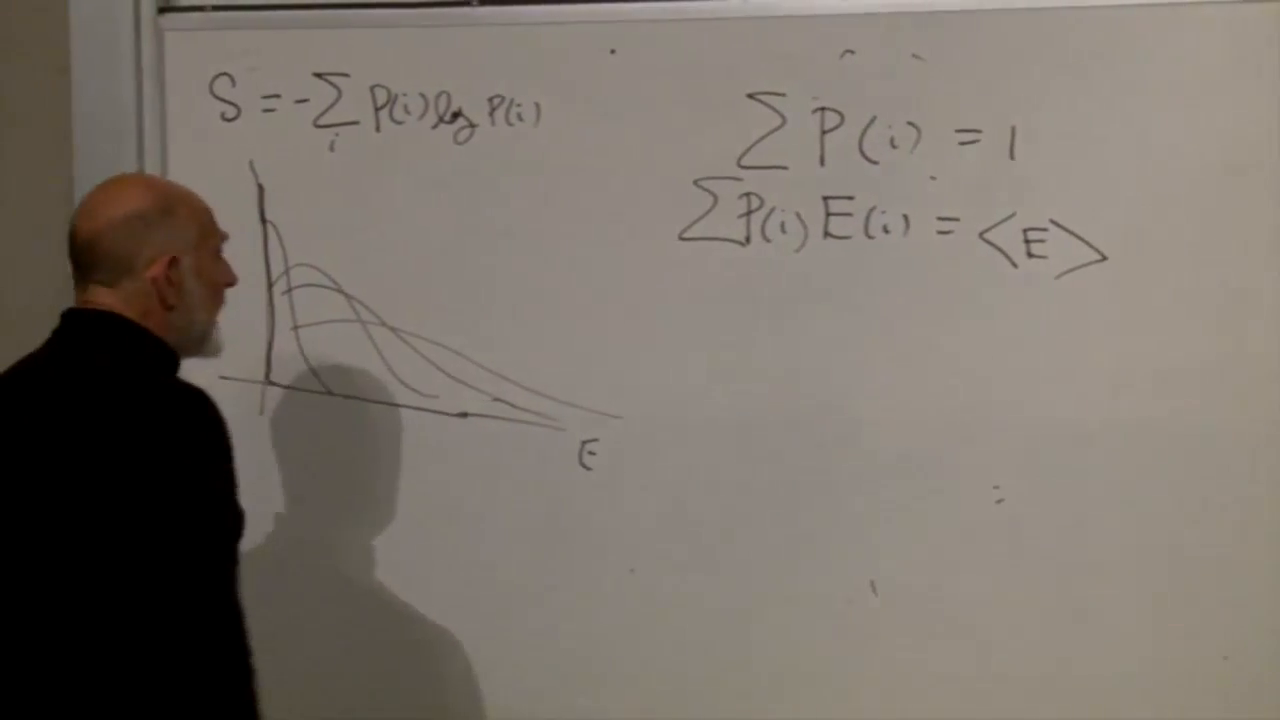
\includegraphics[width=0.88\textwidth]{lecture_03_figure_02.png}\caption{첫 번째 칠판에는 엔트로피, 정규화, 평균 에너지 공식과 평형 분포의 정성적인 모음이 함께 정리되어 있다.}\lectureframe{00:06:44}\end{figure}

\section{분포의 계로 나타낸 평형}

앞선 강의에서는 한 매개변수로 표시되는 평형 분포의 계를 살펴보았다. 이 계를 온도로 나타낼 수도 있지만, 지금은 평균 에너지 \(\overline E\)로 나타내는 편이 더 유용하다. 가능한 최저 에너지에서는 분포가 바닥 상태 하나에 집중된다.
\[
 P_i=\delta_{i0}.
\]이때 상태에 불확실성이 없으므로 \(S=0\)이다. 평형 분포가 더 많은 에너지 준위에 걸쳐 퍼질수록 평균 에너지와 엔트로피는 모두 증가한다.

이는 열적 계에 관한 진술이지, 임의로 만들 수 있는 모든 분포 계에 관한 진술은 아니다. 임의의 계라면 에너지가 커지는 동시에 분포가 좁아질 수도 있다. 여기서 유도할 평형 분포는 보통의 양의 온도 영역에서 그렇게 거동하지 않는다. 이 계를 따라서는
\begin{equation}
 \frac{dS}{d\overline E}>0.
 \label{eq:sm3-positive-temperature-branch}
\end{equation}스펙트럼에 상한이 있는 계에는 이 도함수가 음수가 되는 가지도 있을 수 있다. 그런 음의 온도 영역도 실제로 존재하지만, 여기서는 논의에서 제외한다.

열평형은 미시적인 정지 상태보다 더 넓은 뜻을 지닌다. 분자는 계속 움직이고, 충돌하며, 에너지를 주고받는다. 정지한 것은 거시적 기술이다. 분포에 순방향 변화가 더는 없고, 계의 서로 떨어진 부분 사이에 순 에너지 흐름도 더는 유지되지 않는다.

\section{열역학 법칙을 통계역학의 언어로}

제1법칙은 에너지 보존이다. 제2법칙에 따르면 고립된 거시계의 열역학적 엔트로피는 감소하지 않는다.
\begin{equation}
 \Delta S_{\mathrm{tot}}\geq0.
 \label{eq:sm3-second-law}
\end{equation}등호는 평형 상태나 이상적인 가역 변화를 나타내고, 자발적인 완화에서는 보통 엄격한 증가가 일어난다.

확률적 관점에서 완화가 일어나면 우리가 구별하는 거시적 대안들에 걸친 가중치가 퍼지는 경향이 있다. 여기에는 강의에서 강조한 단서가 필요하다. 우리는 \emph{거친 입자화}를 하고 있다. 정확한 해밀턴 시간발전은 세밀한 위상공간 엔트로피를 보존한다. 미시적 상관관계와 세부 사항을 더 이상 추적하지 않기 때문에 거시적 엔트로피가 증가한다. 이렇게 정보를 잃으면 축약된 기술은 더 넓어진다. 자발적으로 분포가 좁아진다면 측정도 하지 않은 채 미시적 정보를 알아낸 셈이 된다.

영 법칙은 계들이 열평형에 도달할 수 있고, 평형 관계가 추이적임을 말한다. \(A\)가 \(B\)와 평형을 이루고, \(B\)가 \(C\)와 평형을 이룬다면, \(A\)는 \(C\)와 평형을 이룬다. 온도는 이러한 추이성을 명확하게 보여 주는 수를 제공한다:
\[
 T_A=T_B,\qquad T_B=T_C
 \quad\Longrightarrow\quad
 T_A=T_C.
\]
평형 상태가 아니면 에너지는 온도가 더 높은 부분계에서 더 낮은 부분계로 흐른다. 온도가 같아지면 순흐름은 멈춘다. 이제 온도의 엔트로피 정의로부터 이 조작적 진술을 유도해 보자.

\section{에너지는 왜 뜨거운 곳에서 차가운 곳으로 흐르는가}

약하게 결합된 두 부분 계 \(A\)와 \(B\)를 생각하자. 각 부분 계는 내부적으로 평형 상태에 있지만 온도는 서로 다르다. 다음과 같이 기호를 정하자.
\begin{equation}
 T_B>T_A>0.
 \label{eq:sm3-temperature-order}
\end{equation}작은 에너지 교환이 일어나는 동안 전체 에너지 보존에 따라
\begin{equation}
 dE_A+dE_B=0.
 \label{eq:sm3-energy-conservation}
\end{equation}제2법칙에 따르면
\begin{equation}
 dS_A+dS_B\geq0.
 \label{eq:sm3-entropy-change}
\end{equation}내부적으로 평형인 각 부분 계에서 온도는 다음과 같이 정의된다.
\begin{equation}
 dE_X=T_X\,dS_X,
 \qquad X=A,B.
 \label{eq:sm3-temperature-differential}
\end{equation}\eqref{eq:sm3-energy-conservation}을 대입하면
\begin{equation}
 T_A\,dS_A+T_B\,dS_B=0,
\end{equation}따라서
\begin{equation}
 dS_B=-\frac{T_A}{T_B}\,dS_A.
 \label{eq:sm3-dsb}
\end{equation}이 결과를 \eqref{eq:sm3-entropy-change}에 넣으면
\begin{align}
 dS_{\mathrm{tot}}
 &=dS_A-\frac{T_A}{T_B}dS_A\\
 &=\frac{T_B-T_A}{T_B}\,dS_A\geq0.
 \label{eq:sm3-flow-entropy}
\end{align}\(T_B-T_A>0\)이고 \(T_B>0\)이므로 자발적인 교환에는 다음 조건이 필요하다.
\[
 dS_A>0.
\]\eqref{eq:sm3-temperature-differential}에 따라
\begin{equation}
 dE_A=T_A\,dS_A>0,
 \qquad
 dE_B=-dE_A<0.
 \label{eq:sm3-hot-to-cold}
\end{equation}에너지는 더 뜨거운 부분 계인 \(B\)에서 더 차가운 부분 계인 \(A\)로 흘렀다. 여기서 열은 단순히 이동 중인 에너지다. \(T_A=T_B\)가 될 때까지 흐름은 계속된다. 그때는 1차 엔트로피 변화가 어느 한쪽 방향도 더는 선호하지 않는다.

같은 결과를 한 줄로 쓸 수 있다.
\begin{equation}
 dS_{\mathrm{tot}}
 =dE_A\left(\frac{1}{T_A}-\frac{1}{T_B}\right)\geq0.
 \label{eq:sm3-compact-flow}
\end{equation}역온도 차의 부호가 \(dE_A\)의 부호를 결정한다. 이 간결한 형태는 뒤에서 정준 앙상블과 자연스럽게 연결된다.

\begin{classroomqa}\audiencequestion{이 논증은 \(A\)와 \(B\)가 각각 이미 내부 평형 상태라고 가정하나요?}\lecturerresponse{그렇습니다. 하나의 \(T_A\) 또는 \(T_B\)를 부여하는 것 자체가 그 가정을 뜻합니다. 부분 계가 내부 평형이 아니라면, 더 작은 영역들로 나누어 온도를 정의할 수 있는 곳마다 국소적으로 이 논증을 적용하면 됩니다. 그러면 전체적인 완화는 그 영역들 사이의 에너지 교환을 모아 설명할 수 있습니다.
\lecturetimestamp{00:24:38--00:25:22}}\end{classroomqa}

\section{상태란 무엇인가?}

평형 확률을 묻기 전에 표지 \(i\)가 무엇을 뜻하는지 알아야 한다. 미시 상태란 물리 법칙이 허용하는 범위에서 계를 가장 완전하게 규정한 것이다. 고전역학에서는 모든 입자의 위치와 운동량을 떠올리면 된다. 양자역학에서 상태는 그 대신 완전한 양자 상태를 뜻한다. 불확정성 원리 때문에 고전적인 위치와 운동량을 모두 동시에 정확히 지정할 수는 없다.

유한한 상자 안의 양자계에서는 관련 상태 수가 이산적일 수 있다. 적절한 극한에서 촘촘히 놓인 양자 상태의 합이 위상공간 적분으로 바뀌면 고전 통계역학이 얻어진다. 이 극한 과정에서는 연속적인 엔트로피를 무차원으로 만들 위상공간 셀도 도입된다. 단순히 합 기호를 적분 기호로 바꾸는 것만으로 얻어지는 것은 아니다.

\begin{classroomqa}\audiencequestion{기체에서는 모든 분자의 위치와 운동량을 상태로 생각해야 하나요?}\lecturerresponse{고전적인 관점에서는 그렇다. 더 일반적으로 상태란 물리 법칙이 허용하는 범위에서 원칙적으로 계에 대해 알 수 있는 모든 것을 뜻한다. 양자역학에서는 이러한 최대한의 기술 방식이 달라지고, 유한 부피에서의 상태 수는 이산적으로 세어진다. 양자 합에서 고전 적분을 얻는 것은 실제 극한 논증이지, 한 줄짜리 치환이 아니다.
\lecturetimestamp{00:25:31--00:27:38}}\end{classroomqa}

\section{복제 계로 이루어진 열저장고}

이제 핵심 질문을 피할 수 없다. 평형이 성립한 뒤 \(P_i\)를 결정하는 것은 무엇인가?

부분 계를 매우 큰 열저장고와 접촉시켜 보자. 에너지는 오갈 수 있지만, 열저장고에는 자유도가 아주 많으므로 소량의 에너지 이동은 온도를 거의 바꾸지 않는다. 특히 편리한 열저장고는 부분 계 자체를 약하게 결합한 복제 계들로 많이 모아 구성할 수 있다. 복제 계 하나가 연구 대상인 계이고, 나머지는 그 환경을 이룬다.

이 구성은 실제 거시계를 본뜨는 경우가 많다. 거의 균일한 큰 물체를 비슷한 여러 셀로 나눈다고 하자. 각 셀은 부분 계이고 나머지 셀들은 그 셀의 열저장고 역할을 한다. 복제 계의 전체 수를 \(N\)로 나타내자. 수업 중 시연에서는 복제 계 아홉 개와 색으로 구분한 상태 표지 세 개를 사용하지만, 계수 결과는 그 구체적인 수와 무관하다.

상태 \(i\)에 있는 복제 계의 수를 \(n_i\)로 두자. 이를 \emph{점유수}라 한다. 가능한 에너지 준위가 무한히 많더라도 전체 에너지가 유한하면 매우 높은 준위의 점유수는 대부분 무시할 수 있거나 0이다.

첫 번째 제약은 복제 계의 수다.
\begin{equation}
 \sum_i n_i=N.
 \label{eq:sm3-number-constraint}
\end{equation}두 번째 제약은 총에너지다.
\begin{equation}
 \sum_i n_iE_i=N\overline E.
 \label{eq:sm3-total-energy-constraint}
\end{equation}우변은 가산적이다. 통계적 상태를 그대로 유지하면서 복제 계의 수를 두 배로 늘리면 총에너지는 두 배가 되지만 복제 계 하나당 평균 에너지는 \(\overline E\)로 유지된다.

\begin{classroomqa}\audiencequestion{복제 계 구성에서도 에너지 제약을 만족해야 하나요?}\lecturerresponse{그렇다. 점유수의 합은 \(N\)이어야 하고, 점유수에 에너지를 가중해 합한 값은 고정된 총에너지 \(N\overline E\)와 같아야 한다. 뒤에서 엔트로피 최대값을 제한하는 조건은 바로 이 두 가지다.
\lecturetimestamp{00:37:12--00:39:54}}\end{classroomqa}

무작위로 선택한 복제 계가 상태 \(i\)를 차지할 확률은 그 상대 도수다.
\begin{equation}
 P_i=\frac{n_i}{N},
 \qquad
 n_i=NP_i.
 \label{eq:sm3-frequency-probability}
\end{equation}

\begin{figure}[t]\centering
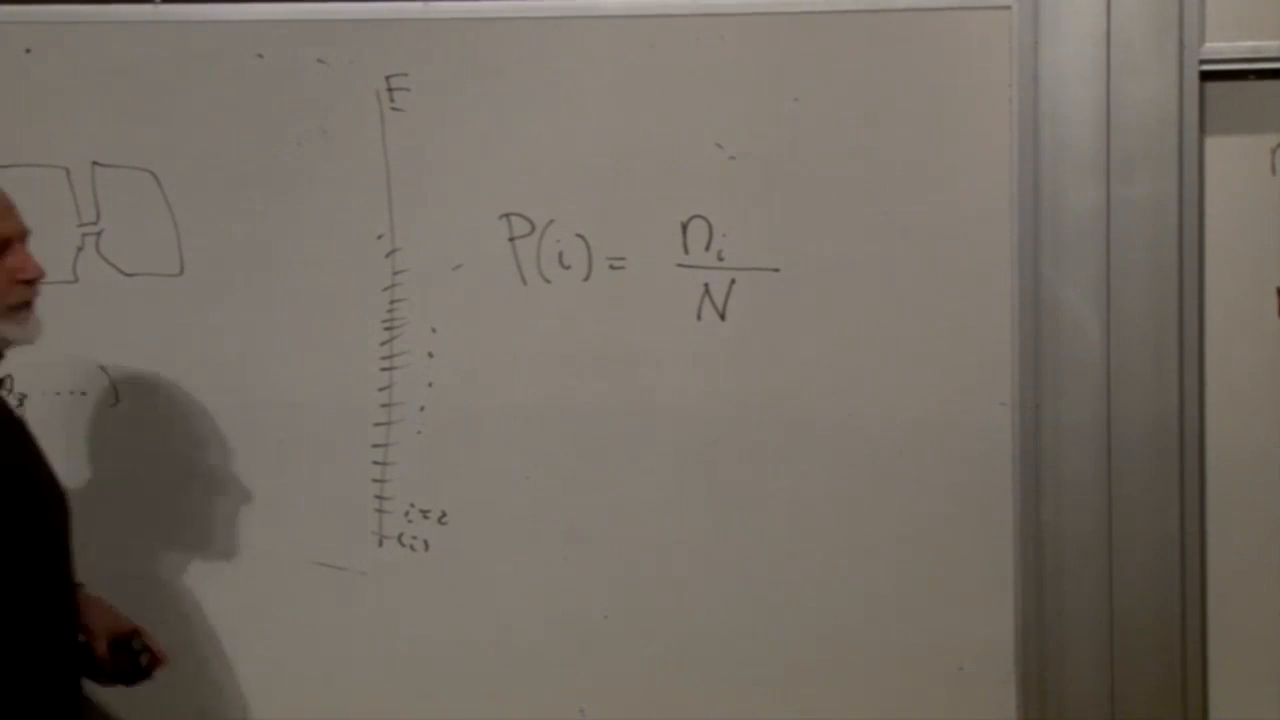
\includegraphics[width=0.82\textwidth]{lecture_03_figure_03.png}\caption{에너지 준위 그림과 점유 비율을 확률로 보는 해석 \(P_i=n_i/N\).}\lectureframe{00:41:40}\end{figure}

\begin{classroomqa}\audiencequestion{칠판의 표기 \(N(i)\)는 \(n_i\)와 다른 뜻인가요?}\lecturerresponse{아니다. 둘 다 상태 \(i\)의 점유수를 나타낸다. 일관되게 \(n_i\)를 사용하고 복제 계의 총수에는 대문자 \(N\)를 쓰기로 하자.
\lecturetimestamp{00:41:28--00:41:33}}\end{classroomqa}

\eqref{eq:sm3-number-constraint}와 \eqref{eq:sm3-total-energy-constraint}를 \(N\)로 나누면 확률 제약 조건이 다시 나온다.
\begin{equation}
 \sum_iP_i=1,
 \qquad
 \sum_iP_iE_i=\overline E.
 \label{eq:sm3-probability-constraints}
\end{equation}따라서 앙상블의 상대 도수 해석으로 처음에 세웠던 방정식을 다시 얻었다.

\section{점유 패턴의 중복도}

점유수 집합 \(\{n_i\}\)를 고정하자. 서로 구별되는 \(N\)개의 복제 계를 상태들에 배정해 정확히 그 집합을 실현하는 방법은 몇 가지일까? 답은 다항계수다.
\begin{equation}
 C(\{n_i\})=\frac{N!}{\prod_i n_i!}.
 \label{eq:sm3-multiplicity}
\end{equation}분모가 생기는 이유를 살펴보자. 먼저 표지가 붙은 복제 계 \(N\)개를 모두 \(N!\)가지 순서로 배열한다. 같은 상태에 있는 \(n_i\)개의 복제 계끼리 자리를 바꾸어도 새로운 점유 배정이 되지 않으므로 각 상태마다 \(n_i!\)로 나눈다.

\begin{figure}[t]\centering
\includegraphics[width=0.88\textwidth]{lecture_03_figure_04.png}\caption{칠판에 적힌 다항 중복도 \(C=N!/\prod_i n_i!\).}\lectureframe{00:46:55}\end{figure}

점유되지 않은 준위는 \(0!=1\)이므로 문제가 되지 않는다. 모든 복제 계가 한 상태에 있다면
\[
 C=\frac{N!}{N!}=1,
\]예상한 대로다. 세 복제 계가 서로 다른 세 지정 상태를 차지한다면
\[
 C=\frac{3!}{1!\,1!\,1!}=6.
\]두 복제 계가 서로 다른 지정 상태 두 개를 차지하는 경우에는 두 가지 배정이 나온다. 표지가 붙은 두 복제 계가 각각 어느 상태를 차지하는지를 맞바꾸면 된다.

\begin{classroomqa}\audiencequestion{두 제약 조건을 만족하는 점유수 집합이 여러 개일 수 있나요?}\lecturerresponse{대개 여러 집합이 가능하다. 식 \eqref{eq:sm3-multiplicity}은 먼저 제약 조건을 만족하는지 따지지 않고, 고정된 한 집합 \(\{n_i\}\)에 대한 배열 수를 센다. 다음 단계에서는 제약 조건과 양립하는 모든 집합을 비교해 중복도가 가장 큰 것을 찾는다.
\lecturetimestamp{00:48:07--00:48:43}}\end{classroomqa}

통계적 가정은 고립된 설정과 양립하는 미시적 배정들을 동등하게 취급한다는 것이다. 따라서 더 많은 배정으로 실현되는 거시적 점유 패턴이 더 높은 확률을 갖는다. \(N\)가 클 때 비율 \(n_i/N\)의 분포는 뚜렷한 최빈값 주위에 집중된다. 평형 비율은 \eqref{eq:sm3-number-constraint}와 \eqref{eq:sm3-total-energy-constraint}를 만족하는 조건 아래 \(C\)을 최대화하는 값이다.

\section{스털링 근사}

계승은 \(N\)이 거시적인 값에 도달하기 훨씬 전부터 엄청나게 커지므로, 로그를 취해 다룬다. 다음 식에서 시작하자.
\begin{equation}
 \log N!=\sum_{x=1}^{N}\log x.
 \label{eq:sm3-log-factorial-sum}
\end{equation}
\(N\)이 클 때 이 합은 \(\log x\) 곡선 아래의 넓이로 근사된다.
\begin{align}
 \log N!
 &\simeq\int_1^N\log x\,dx\\
 &=\left[x\log x-x\right]_1^N\\
 &=N\log N-N+1.
 \label{eq:sm3-stirling-integral}
\end{align}
부정적분은 다음 식에서 바로 구할 수 있다.
\[
 \frac{d}{dx}(x\log x-x)=\log x.
\]
계의 크기에 비례하는 선도 차수에서는 가산 상수를 생략해도 된다.
\begin{equation}
 \log N!\simeq N\log N-N.
 \label{eq:sm3-stirling-log}
\end{equation}
양변을 지수화하면 강의에서 사용한 간단한 형태를 얻는다.
\begin{equation}
 N!\simeq N^N e^{-N}.
 \label{eq:sm3-stirling-simple}
\end{equation}

\begin{figure}[t]\centering
\includegraphics[width=0.88\textwidth]{lecture_03_figure_05.png}\caption{합 \(\log x\)을 적분으로 바꾸어 유도한 스털링 근사의 선도항.}\lectureframe{01:03:45}\end{figure}

\begin{classroomqa}\audiencequestion{하한에서 \(x\log x-x\)을 계산하면 \(+1\)가 더 남지 않나요?}\lecturerresponse{그렇다. 식 \eqref{eq:sm3-stirling-integral}에는 그 상수가 들어 있다. \(N\to\infty\)일 때 \(N\)에 비례하는 항들에 비하면 무시할 수 있으므로 선도 근사식에서는 생략한다. 합은 반드시 \(x=1\)에서 시작해야 한다. \(\log0\)는 정의되지 않는다.
\lecturetimestamp{01:04:12--01:04:35}}\end{classroomqa}

\begin{classroomqa}\audiencequestion{\(\sqrt{N}\)에 비례하는 인자도 빠진 것 아닌가요?}\lecturerresponse{그렇다. 더 정확한 점근식은 다음과 같다.
\[
 N!\sim\sqrt{2\pi N}\left(\frac{N}{e}\right)^N.
\]로그를 취하면 \(\tfrac12\log(2\pi N)\)만 추가되는데, 이는 \(N\log N-N\)에 비해 비가산적이다. 유한한 \(N\)에서 확률을 정확히 계산할 때는 중요하지만, 거시계의 엔트로피를 선도 차수에서 계산할 때는 중요하지 않다.
\lecturetimestamp{01:04:35--01:05:40}}\end{classroomqa}

\eqref{eq:sm3-multiplicity}의 분모에 스털링 근사를 적용할 때도 주의해야 한다. 열역학적 극한에서 극한 확률이 양수인 상태들은 \(n_i=NP_i\)를 만족하므로, 그 점유수는 \(N\)에 비례해 커진다. 점유수가 매우 작거나 사라지는 상태는 유한한 에너지 절단을 도입해 다룬 뒤 극한을 취해 복원할 수 있다. 생략한 차수 낮은 항들은 선도적인 광범위 엔트로피에 영향을 주지 않는다.

\section{중복도의 로그가 엔트로피다}

분자와 거시적으로 점유된 모든 분모 인자에 \eqref{eq:sm3-stirling-simple}를 적용하면
\begin{equation}
 C\simeq
 \frac{N^Ne^{-N}}
 {\prod_i n_i^{\,n_i}e^{-n_i}}.
 \label{eq:sm3-c-stirling}
\end{equation}\(\sum_i n_i=N\)이므로 선도 지수 인자들이 상쇄된다.
\begin{equation}
 C\simeq\frac{N^N}{\prod_i n_i^{\,n_i}}.
 \label{eq:sm3-c-leading}
\end{equation}곱보다 로그를 최대화하기가 쉽고 로그는 단조 함수이므로 두 경우의 최댓값은 같은 점유 패턴에서 얻어진다.
\begin{equation}
 \log C=N\log N-\sum_i n_i\log n_i.
 \label{eq:sm3-logc-occupations}
\end{equation}이제 \(n_i=NP_i\)를 대입하면
\begin{align}
 \log C
 &=N\log N-\sum_iNP_i\log(NP_i)\\
 &=N\log N-N\sum_iP_i\log N
   -N\sum_iP_i\log P_i\\
 &=-N\sum_iP_i\log P_i,
 \label{eq:sm3-logc-entropy-derivation}
\end{align}정규화 조건에 의해 두 \(N\log N\) 항이 상쇄된다. 따라서 \(N\)의 선도 차수에서
\begin{equation}
 \boxed{\log C=NS}.
 \label{eq:sm3-logc-ns}
\end{equation}

\begin{figure}[t]\centering
\includegraphics[width=0.88\textwidth]{lecture_03_figure_06.png}\caption{칠판 계산: \(\log C=N\log N-\sum_i n_i\log n_i\)를 \(-N\sum_iP_i\log P_i=NS\)와 연결한다.}\lectureframe{01:16:10}\end{figure}

이 관계는 이 장의 핵심이다. 엔트로피는 계수 문제에 별도로 덧붙인 무관한 양이 아니다. 엔트로피는 복제 계 하나당 중복도를 로그로 측정한 것이다. 따라서 선도 차수에서 미시적 배열의 수를 최대화하는 것은 복제 계 하나의 엔트로피를 최대화하는 것과 같다.

\begin{classroomqa}\audiencequestion{점유수가 모두 같을 때 중복도가 가장 크지 않나요?}\lecturerresponse{어떤 상태도 특별히 구별되지 않고 유한한 상태 집합에서 \(\sum_i n_i=N\)만 부과될 때는 균일 분포가 된다. 고정 에너지 제약이 답을 바꾸는 이유는 \(E_i\)의 값이 서로 다르기 때문이다. 일반적으로 점유수를 같게 하면 지정된 평균 에너지를 얻을 수 없다.
\lecturetimestamp{01:17:07--01:18:20}}\end{classroomqa}

\begin{classroomqa}\audiencequestion{수 \(N\)는 크지만, 분모의 모든 \(n_i\)에 스털링 근사를 적용해도 되는 이유는 무엇인가?}\lecturerresponse{극한 확률이 양수인 각 상태에서는 \(n_i=NP_i\)가 \(N\)에 비례해 커집니다. 먼저 유한한 에너지 범위만 남겨 그 범위에서 \(N\)가 커지는 극한을 취한 다음, 에너지 범위를 넓힐 수 있습니다. 꼬리 부분의 희소한 상태들은 별도의 유한한 보정이 필요하지만, 선도적인 광범위 엔트로피를 바꾸지는 않습니다.
\lecturetimestamp{01:18:23--01:19:28}}
\end{classroomqa}

\begin{classroomqa}\audiencequestion{앞서 말한 거친 입자화가 바로 이 큰 \(N\) 근사를 뜻하나요?}\lecturerresponse{아니다. 열역학적 극한은 큰 점유수와 점근적 계수를 다룬다. 거친 입자화는 미시적 분해능을 잃거나 의도적으로 버리는 일이다. 거시적 통계역학에서 둘 다 자주 쓰이지만, 서로 다른 연산이다.
\lecturetimestamp{01:19:29--01:19:46}}\end{classroomqa}

\begin{classroomqa}\audiencequestion{\(\log C=N\log N-\sum_i n_i\log n_i\)이므로 두 번째 항을 최대화하는 대신 최소화해야 하나요?}\lecturerresponse{그렇다. \(N\)를 고정하면 \(\log C\)를 최대화하는 것은 \(\sum_i n_i\log n_i\)를 최소화하는 것과 같다. \(n_i=NP_i\)를 대입하면 고정된 \(N\log N\) 항들이 상쇄되고 \(-N\sum_iP_i\log P_i=NS\)만 남는다. 따라서 이를 양의 엔트로피 \(S\)를 최대화하는 것으로 표현하는 편이 더 자연스럽다.
\lecturetimestamp{01:19:48--01:20:55}}\end{classroomqa}

\begin{classroomqa}\audiencequestion{대칭성을 이용해 곧바로 모든 \(n_i\)를 같게 두면 안 되나요?}\lecturerresponse{그렇게 하면 에너지 표지를 무시하게 된다. 정규화 제약은 상태들을 대칭적으로 다루지만 \(\sum_iP_iE_i=\overline E\)는 그렇지 않다. 에너지가 다른 상태들은 서로 다르게 기여한다. 에너지 제약이 바로 비균일한 평형 분포를 결정한다.
\lecturetimestamp{01:21:15--01:21:41}}\end{classroomqa}

\section{최대 엔트로피 문제}

이제 통계역학의 규칙을 모호함 없이 쓸 수 있다. 확률 \(P_i\)를 변화시켜
\begin{equation}
 S[P]=-\sum_iP_i\log P_i
 \label{eq:sm3-maximize-entropy}
\end{equation}를 최대화한다. 단, 다음 조건을 만족해야 한다.
\begin{equation}
 \sum_iP_i=1,
 \qquad
 \sum_iP_iE_i=\overline E.
 \label{eq:sm3-maxent-constraints}
\end{equation}최대화된 확률은 큰 복제 앙상블에서 뚜렷하게 선호되는 점유 비율을 준다. 점유수는 요동하지만 \(N\)가 커질수록 상대 편차는 줄어들어 비율 \(n_i/N\)가 잘 정의된 열역학적 확률이 된다.

\begin{classroomqa}\audiencequestion{\(E_i\)는 고정된 상태 에너지이고, 제약 조건에는 별도로 주어진 총에너지를 쓰나요?}\lecturerresponse{그렇다. 스펙트럼 \(\{E_i\}\)는 부분 계의 고유한 성질이다. 복제 계 전체의 총에너지는 고정되어 있지만, 에너지는 복제 계들 사이에서 계속 이동한다. 총에너지를 \(N\)로 나누면 복제 계 하나의 평균 에너지 \(\overline E\)가 정해질 뿐, 개별 미시적 실현에서 복제 계의 에너지가 정해지는 것은 아니다.
\lecturetimestamp{01:26:12--01:27:07}}\end{classroomqa}

문제는 쉽게 쓸 수 있지만 아직 풀리지는 않았다. 제약 조건이 두 개인 극값 문제이므로 수학적 도구가 하나 더 필요하다.

\section{라그랑주 승수}

제약이 없는 함수 \(F(x_1,x_2,\ldots)\)의 정지점은 다음을 만족한다.
\begin{equation}
 \frac{\partial F}{\partial x_i}=0
 \qquad\text{for every }i.
 \label{eq:sm3-unconstrained-stationary}
\end{equation}이제 추가로 다음 조건을 요구하자.
\begin{equation}
 G(x_1,x_2,\ldots)=0.
 \label{eq:sm3-one-constraint}
\end{equation}

\begin{classroomqa}\audiencequestion{그림의 좌표가 \(x\)와 \(y\)라면 \(x\)는 무엇을 뜻하나요?}\lecturerresponse{여기서 \(x\)은 좌표 벡터 전체 \((x_1,x_2,\ldots)\)를 간단히 나타낸 것이다. 이차원 그림에서는 성분이 \(x\)와 \(y\)뿐이다. 나중에는 성분이 확률 \(P_1,P_2,\ldots\)가 된다.
\lecturetimestamp{01:30:12--01:30:20}}\end{classroomqa}

기하학적으로 보면 곡면 \(F=\text{constant}\)은 등고선도이고, \(G=0\)은 계가 따라 움직일 수 있는 곡선이다. 제약된 극값은 \(F\)의 한 등고선이 제약 곡선에 접할 때 생긴다. 그 지점에서 기울기 벡터들은 서로 평행하다.
\begin{equation}
 \nabla F=-\lambda\nabla G
 \label{eq:sm3-parallel-gradients}
\end{equation}어떤 수 \(\lambda\)에 대하여 성립한다.

\begin{figure}[t]\centering
\includegraphics[width=0.88\textwidth]{lecture_03_figure_07.png}\caption{칠판에 그린 등고선의 기하학적 관계와 확장 함수 \(F'=F+\lambda G\). 접점에서 제약된 극값이 생긴다.}\lectureframe{01:37:10}\end{figure}

확장 함수
\begin{equation}
 F'=F+\lambda G
 \label{eq:sm3-augmented-function}
\end{equation}를 정의하고 보통의 정지 조건을 요구하면 식 \eqref{eq:sm3-parallel-gradients}를 얻을 수 있다.
\begin{equation}
 \frac{\partial F'}{\partial x_i}=0.
 \label{eq:sm3-augmented-stationarity}
\end{equation}승수 \(\lambda\)는 처음에는 미지수다. 그렇다고 연립 문제가 미정인 것은 아니다. 원래의 제약 조건 \(G=0\)이 방정식 하나를 더 제공한다.

\begin{classroomqa}\classquestion{\(G\)에 비례하는 항을 더하면 왜 제약된 점에서 정지하게 되나요?}\lecturerresponse{제약된 극값에서는 \(G=0\)에 접하는 방향으로 움직여도 \(F\)가 1차에서 변하지 않는다. 남은 기울기는 제약에 수직인 방향뿐이다. \(\nabla G\)는 바로 그 수직 방향을 가리키므로 적절한 \(\lambda\)를 택해 그 기울기를 상쇄할 수 있다.
\(\nabla F+\lambda\nabla G=0\).
\lecturetimestamp{01:35:06--01:35:32}}\end{classroomqa}

\section{두 변수 예제}

다음을 최소화하자.
\begin{equation}
 F(x,y)=\frac{x^2+y^2}{2}
 \label{eq:sm3-example-f}
\end{equation}단, 다음 조건을 만족해야 한다.
\begin{equation}
 x+y=1.
 \label{eq:sm3-example-constraint}
\end{equation}제약 조건을 \(G=x+y-1=0\)으로 쓰고 다음을 구성한다.
\begin{equation}
 F'=\frac{x^2+y^2}{2}+\lambda(x+y-1).
 \label{eq:sm3-example-augmented}
\end{equation}정지 조건은 다음과 같다.
\begin{align}
 \frac{\partial F'}{\partial x}&=x+\lambda=0,\\
 \frac{\partial F'}{\partial y}&=y+\lambda=0.
 \label{eq:sm3-example-derivatives}
\end{align}따라서 \(x=y=-\lambda\)이다. 남은 방정식은 제약 조건이다.
\[
 x+y=-2\lambda=1,
\]그러므로
\begin{equation}
 \lambda=-\frac12,
 \qquad
 x=y=\frac12.
 \label{eq:sm3-example-solution}
\end{equation}점 \((1/2,1/2)\)은 원점을 중심으로 하는 가장 작은 원이 직선 \(x+y=1\)에 접하는 지점이다.

\begin{figure}[t]\centering
\includegraphics[width=0.88\textwidth]{lecture_03_figure_08.png}\caption{\(x+y=1\) 조건 아래 \((x^2+y^2)/2\)을 최소화하는 라그랑주 승수 계산의 전체 과정.}\lectureframe{01:44:10}\end{figure}

제약 조건이 여러 개라면 각각에 승수를 하나씩 도입한다.
\begin{equation}
 F'=F+\lambda_1G_1+\lambda_2G_2+\cdots.
 \label{eq:sm3-many-multipliers}
\end{equation}그런 다음 다음 조건들을 푼다.
\begin{equation}
 \begin{aligned}
 \frac{\partial F'}{\partial x_i}&=0
 &&\text{for every }i,\\
 G_a&=0
 &&\text{for every constraint }a.
 \end{aligned}
 \label{eq:sm3-many-equations}
\end{equation}강의에서는 일부러 인위적인 연습 문제를 제안한다. \(x,y,z\)의 이차함수에 두 개의 독립적인 선형 제약 조건, 예컨대 \(x+y=1\)와 \(z+x=1\)를 부과해 극값을 구하는 문제다. 목적은 특정한 답을 구하는 데 있지 않다. 제약 조건마다 승수 하나와 방정식 하나가 추가된다는 규칙을 익히는 데 있다.

\section{다음 강의에 풀 문제}

통계역학에서는 좌표가 확률 \(\{P_i\}\)이고, 최대화할 함수가 엔트로피이며, 제약 조건은 정규화와 고정된 평균 에너지다. 다음과 같이 정의하자.
\begin{align}
 S[P]&=-\sum_iP_i\log P_i,\\
 G_1[P]&=\sum_iP_i-1,\\
 G_2[P]&=\sum_iP_iE_i-\overline E.
 \label{eq:sm3-final-functions}
\end{align}따라서 확장 엔트로피는 다음과 같이 쓸 수 있다.
\begin{equation}
 \Phi[P]
 =S[P]+\alpha G_1[P]+\beta G_2[P].
 \label{eq:sm3-final-augmented}
\end{equation}풀어야 할 방정식은 다음과 같다.
\begin{equation}
 \frac{\partial\Phi}{\partial P_i}=0
 \quad\text{for every }i,
 \qquad
 G_1=0,
 \qquad
 G_2=0.
 \label{eq:sm3-final-problem}
\end{equation}

\begin{figure}[H]\centering
\includegraphics[width=0.88\textwidth]{lecture_03_figure_09.png}\caption{마지막 칠판: 확률의 함수로 표현한 엔트로피와 정규화 및 고정 평균 에너지 조건.}\lectureframe{01:53:05}\end{figure}

이제 문제를 완전히 설정했다. \eqref{eq:sm3-final-problem}을 풀면 평형 분포가 나온다. 에너지에 켤레인 승수는 \(\beta=1/T\)가 되며, 그 부호는 \eqref{eq:sm3-final-augmented}에서 선택한 부호 규약에 따른다. 다음 강의에서는 이 미분을 수행해 볼츠만 가중치를 얻는다.
\chapter{볼츠만 가중치, 분배함수, 이상기체}

\lectureoverview{정규화와 평균 에너지를 고정한 채 엔트로피를 최대화하여 평형 확률 분포를 유도한다. 이어서 분배함수를 미분하면 평균 에너지, 엔트로피, 온도를 얻는다. 이상기체를 첫 번째 완전한 예로 살펴본 뒤, 중력장으로 확장하고 에너지 요동을 간략히 예고한다.}

\section{제약 조건이 있는 엔트로피 문제}

같은 부분계의 상호작용이 매우 약한 복제본 \(\mathcal N\)개가 모인 큰 집합에서 시작하자. \(n_i\)개의 복제본이 \(i\)번째 상태에 있다면, \begin{equation}
 p_i=\frac{n_i}{\mathcal N},
 \qquad
 \sum_i p_i=1.
 \label{eq:sm4-occupation-probability}
\end{equation}앞 강의의 다항계수 계산으로 복제본 하나당 엔트로피를 얻는다. \begin{equation}
 S[p]=-\sum_i p_i\log p_i.
 \label{eq:sm4-entropy}
\end{equation}이를 모든 변수 \(p_1,p_2,\ldots\)의 보통 함수로 보는 것이 좋다. 계산을 가능하게 하는 것은 이 함수의 단순한 가법 형태다.

복제본 집합의 전체 에너지는 \(\mathcal N E\)로 고정되어 있으며, 여기서 \(E\)는 복제본 하나당 평균 에너지다. 따라서 두 번째 제약 조건은 \begin{equation}
 \sum_i p_iE_i=E.
 \label{eq:sm4-energy-constraint}
\end{equation}\(E_i\)는 부분계의 에너지 준위이고, 우변의 \(E\)은 확률로 가중한 준위의 평균이다. \eqref{eq:sm4-entropy}을 \eqref{eq:sm4-occupation-probability} 및 \eqref{eq:sm4-energy-constraint}의 조건 아래 최대화하면 점유율 가운데 압도적으로 가장 가능성이 높은 값이 선택된다.

편의상 \(-S=\sum_i p_i\log p_i\)를 최소화하자. 각 제약 조건에 라그랑주 승수를 하나씩 도입하면 다음과 같다. \begin{equation}
 \begin{aligned}
 \Phi[p;\alpha,\beta]
 &=\sum_i p_i\log p_i\\
 &\quad+\alpha\left(\sum_i p_i-1\right)\\
 &\quad+\beta\left(\sum_i p_iE_i-E\right).
 \end{aligned}
 \label{eq:sm4-augmented-functional}
\end{equation}\(\alpha\)와 \(\beta\)라는 이름은 아직 물리적 가정을 뜻하지 않는다. 이 단계에서는 두 제약 조건을 부과하는 데 필요한 두 수일 뿐이다.

\begin{classroomqa}\audiencequestion{확장된 함수도 \(\alpha\)와 \(\beta\)의 함수인가요?}\lecturerresponse{그렇습니다. 이 함수에 대해 \(\alpha\)와 \(\beta\)을 변화시키면 두 제약 조건이 다시 얻어집니다. 하지만 지금 계산에서는 승수들을 고정한 채 확률 \(p_i\)를 변화시킵니다. 승수의 값은 정규화 조건과 주어진 평균 에너지로 나중에 정해집니다. \lecturetimestamp{00:09:32--00:09:49}}\end{classroomqa}

\begin{figure}[t]\centering
\includegraphics[width=0.92\textwidth]{lecture_04_figure_02.png}\caption{확률을 변화시킬 때 상수인 항을 생략한 확장 엔트로피 범함수.}\lectureframe{00:10:56}\end{figure}

확률에 대해 미분할 때 \(-\alpha\)와 \(-\beta E\)는 기여하지 않는다. 칠판에 보이는 식은 이렇게 축약된 범함수다. 이 항들은 여전히 \eqref{eq:sm4-augmented-functional}의 일부지만, 이 특정한 미분에서는 더 이상 영향을 주지 않을 뿐이다.

\section{볼츠만 분포}

확률 하나를 임의로 고르자. 강의에서는 \(p_7\)을 택한다. \(1\)은 너무 특별해 보이고 \(7\)은 행운의 수이기도 해서다. 무엇을 택하든 결과는 달라지지 않는다. 필요한 미적분은 다음뿐이다. \begin{equation}
 \frac{d}{dp_i}\bigl(p_i\log p_i\bigr)=\log p_i+1.
\end{equation}따라서 \begin{equation}
 \frac{\partial\Phi}{\partial p_i}
 =\log p_i+1+\alpha+\beta E_i=0.
 \label{eq:sm4-stationarity}
\end{equation}이다. 이를 \(p_i\)에 대해 풀면 \begin{align}
 \log p_i&=-(1+\alpha)-\beta E_i,\\
 p_i&=e^{-(1+\alpha)}e^{-\beta E_i}.
\end{align}를 얻는다. 첫 번째 인자는 상태 표지자와 무관하다. 이를 \(1/Z\)로 쓰면 다음과 같다. \begin{equation}
 p_i=\frac{e^{-\beta E_i}}{Z}.
 \label{eq:sm4-boltzmann-weight}
\end{equation}

이것이 첫 번째 뜻밖의 성과다. 일상적인 제약 미분에서 지수 법칙이 나왔다. 상대 확률은 \begin{equation}
 \frac{p_i}{p_j}=e^{-\beta(E_i-E_j)}.
 \label{eq:sm4-relative-weight}
\end{equation}를 따른다. 승수 \(\beta\)은 에너지가 커질수록 확률이 얼마나 빠르게 감소하는지를 조절한다. \(\beta\)이 큰 양수이면 분포는 가장 낮은 준위에 집중되고, \(\beta\)이 작은 양수이면 스펙트럼에서 더 높은 준위에도 상당한 가중치가 퍼진다. 이미 \(\beta\)을 바꾸면 평균 에너지가 변한다는 것을 알 수 있지만, 이것이 역온도라는 점은 아직 증명해야 한다.

\section{정규화와 분배함수}

정규화 조건으로 상태와 무관한 인자가 정해진다. \begin{equation}
 1=\sum_i p_i
 =\frac{1}{Z}\sum_i e^{-\beta E_i},
\end{equation}따라서 \begin{equation}
 Z(\beta)=\sum_i e^{-\beta E_i}.
 \label{eq:sm4-partition-function}
\end{equation}이다. 이것이 정준 분배함수다. 처음에는 정규화 상수로 등장하지만, 그렇게만 부르면 그 역할을 크게 과소평가하게 된다. \(Z(\beta)\)만 알면 그 미분으로 열역학적 물리량을 구할 수 있다.

\eqref{eq:sm4-partition-function}에 들어가는 에너지 준위는 입력값이다. 에너지 준위는 계의 역학과 고정된 외부 조건, 즉 상자의 부피와 모양, 자기장이나 전기장, 그 밖의 제어 변수에 의해 정해진다. 제어 변수를 바꾸면 스펙트럼이 달라지고, 이에 따라 \(Z\)도 달라진다. 지금 계산에서는 그런 변수들과 그에 따른 집합 \(\{E_i\}\)을 고정한다.

\begin{classroomqa}\audiencequestion{지수함수 그래프의 축은 정확히 무엇을 나타내나요? 세로 좌표는 특정한 \(p_i\)인가요?}\lecturerresponse{그래프의 높이는 각 준위에 부여된 확률이고, 가로축의 순서는 상태 표지자 \(i\)로 읽을 수도 있고 물리적으로는 에너지 \(E_i\)로 읽을 수도 있습니다. 모든 상태의 에너지는 고정되어 있습니다. \(\beta\)이 크면 그 에너지에 따라 확률이 가파르게 감소하고, \(\beta=0\)에 가까우면 접근 가능한 준위들에 거의 균일한 가중치가 부여됩니다. \lecturetimestamp{00:19:39--00:20:09}}\end{classroomqa}

\section{분배함수에 감춰진 평균 에너지}

두 번째 제약 조건으로 \(\beta\)이 정해진다. \begin{equation}
 E=\sum_i p_iE_i
 =\frac{1}{Z}\sum_i E_i e^{-\beta E_i}.
 \label{eq:sm4-mean-energy}
\end{equation}이 가중합을 매번 새로 계산하는 대신 \eqref{eq:sm4-partition-function}을 미분하자. \begin{equation}
 \frac{dZ}{d\beta}
 =-\sum_i E_i e^{-\beta E_i}.
\end{equation}이를 \eqref{eq:sm4-mean-energy}와 비교하면 \begin{equation}
 E(\beta)
 =-\frac{1}{Z}\frac{dZ}{d\beta}
 =-\frac{d\log Z}{d\beta}.
 \label{eq:sm4-energy-logz}
\end{equation}을 얻는다. 로그를 취하는 이유는 그 미분이 \(1/Z\) 인자를 주기 때문이다.

\begin{figure}[t]\centering
\includegraphics[width=0.82\textwidth]{lecture_04_figure_03.png}\caption{정규화 조건, 평균 에너지 제약 조건, 분배함수의 미분이 칠판에 함께 나타나 있다.}\lectureframe{00:26:24}\end{figure}

\begin{classroomqa}\audiencequestion{아래쪽 칠판의 식은 \(Z\)에 관한 새로운 식인가요, 아니면 위 식의 정의에서 얻어지나요?}\lecturerresponse{정의식 \(Z=\sum_i e^{-\beta E_i}\)을 미분해 얻습니다. 미분하면 \(-E_i\)이 내려옵니다. 결과를 \(Z\)로 나누면 평균 에너지를 정의하는 가중합이 다시 나옵니다. \lecturetimestamp{00:25:58--00:26:37}}\end{classroomqa}

\begin{classroomqa}\audiencequestion{\(dZ/d\beta=-E Z\)은 \(Z\)을 미분 연산의 고유함수로 만드나요?}\lecturerresponse{보통 의미에서는 그렇지 않습니다. 고유값 방정식이라면 \(Z\)에 상수가 곱해져야 하지만, 여기서는 \(E=E(\beta)\)입니다. 이 식은 \(\beta\)에 따른 평균 에너지를 알려줄 뿐, 고정된 고유값 문제는 아닙니다. \lecturetimestamp{00:28:49--00:29:43}}\end{classroomqa}

\eqref{eq:sm4-energy-logz}의 단순함은 착각을 불러일으킬 수 있다. 스펙트럼은 복잡할 수 있고 \(Z\)을 계산하기도 어렵지만, 일단 이 함수 하나만 구하면 미분 한 번으로 평균 에너지를 얻는다. 이런 패턴은 통계역학 전반에서 거듭 나타난다. 간단한 연산을 올바른 순서로 적용하면 직접 예상하기 어려운 결과를 얻을 수 있다.

\begin{classroomqa}\audiencequestion{\(E\)는 복제본 전체의 총에너지인가요, 아니면 상자 하나의 평균 에너지인가요?}\lecturerresponse{상자 하나의 평균 에너지입니다. 복제본 집합의 총에너지는 \(\mathcal N E\)입니다. 나중에 계 자체를 \(N\)개의 기체 입자를 담은 상자 하나 전체로 정하면 \(E\)는 기체 표본 전체의 에너지를 뜻합니다. \lecturetimestamp{00:30:55--00:31:10}}\end{classroomqa}

\begin{classroomqa}\audiencequestion{\(\sum_i e^{-\beta E_i}\)의 각 항에 로그를 취해도 되나요?}\lecturerresponse{안 됩니다. 로그는 곱을 합으로 바꾸지만, 합을 로그들의 합으로 바꾸지는 않습니다. \[
 \log\!\left(\sum_i e^{-\beta E_i}\right)
 \ne \sum_i\log\!\left(e^{-\beta E_i}\right).
\]독립적인 부분계들의 분배함수가 곱해지는 경우에는 이 구분이 유용해집니다. \lecturetimestamp{00:31:10--00:31:58}}\end{classroomqa}

\section{무엇이 고정되고 무엇이 변할 수 있는가}

같은 식에 여러 층위의 변수가 등장하므로, 강의에서는 이들을 의도적으로 구분한다.

\begin{itemize}\item 확률 \(p_i\)는 처음에 구하려던 미지수다. \item 준위 \(E_i\)는 계와 제어 변수가 정해지면 고정된다. \item 승수 \(\alpha\)는 정규화 인자 \(Z=e^{1+\alpha}\)에 흡수되었다. \item 주어진 평균 에너지 \(E\)에 대해 제약 조건이 하나의 수 \(\beta\)를 정한다. 하지만 평형 상태들의 한 계열을 보면 \(E=E(\beta)\)이나 \(\beta=\beta(E)\)를 매개변수로 사용할 수 있다. \end{itemize}

\begin{classroomqa}\audiencequestion{승수는 수인데 왜 이제 \(\beta\)와 \(E\)를 변수처럼 다루나요?}\lecturerresponse{하나의 제약 문제에서는 실제로 수입니다. 하지만 스펙트럼은 같고 주어진 평균 에너지는 서로 다른 여러 평형 문제를 비교할 수 있습니다. 그 상태들의 계열을 따라가면 \(\beta\)가 \(E\)에 따라 변합니다. \(E\)를 고정하면 \(\beta\)가 정해지고, \(\beta\)를 고정하면 \(E\)가 정해집니다. 이는 같은 관계를 두 가지 방식으로 읽은 것입니다. \lecturetimestamp{00:31:58--00:33:27}}\end{classroomqa}

\begin{classroomqa}\audiencequestion{\(\alpha\)은 사라졌나요?}\lecturerresponse{이름만 사라졌습니다. 정의식 \(e^{-(1+\alpha)}=1/Z\)에 따라 \(Z\)에 흡수됩니다. \(\alpha\)와 \(Z\)를 모두 남겨두면 같은 정규화 매개변수를 두 번 세게 됩니다. \lecturetimestamp{00:33:29--00:33:49}}\end{classroomqa}

에너지만이 보존량인 것은 아니다. 총운동량, 입자 수, 각운동량 또는 다른 물리량에 제약을 두면 그 기댓값에 각기 고유한 승수를 붙인다. 이렇게 앙상블은 확장되지만 방법은 달라지지 않는다.

\begin{classroomqa}\audiencequestion{평균 에너지만 고정하는 것은 계에 대해 지나친 가정을 하는 것 아닌가요?}\lecturerresponse{현재 문제에서 다른 보존량을 조건으로 둘 필요가 없다고 가정하는 것입니다. 예를 들어 총운동량도 고정한다면 제약 조건과 라그랑주 승수를 하나씩 더하면 됩니다. 반면 부피, 모양, 외부장은 여기서 제어 변수다. 이들은 고정되어 있으며 에너지 준위 자체를 정합니다. \lecturetimestamp{00:33:51--00:35:50}}\end{classroomqa}

\begin{classroomqa}\audiencequestion{\(\alpha\)를 에너지의 또 다른 변수로 넣어야 하나요? 그리고 \(Z\)는 준위 \(E_i\)에 의존하나요?}\lecturerresponse{\(\alpha\)는 이미 \(Z\)에 포함되어 있으므로 독립적인 변수가 아닙니다. 분배함수는 \(\beta\)뿐 아니라 고정된 스펙트럼에도 분명히 의존합니다. 제어 변수를 바꾸면 \(E_i\)이 바뀌고, 따라서 \(Z\)도 바뀝니다. 현재의 \(\beta\) 미분을 하는 동안에는 스펙트럼을 고정합니다. \lecturetimestamp{00:35:52--00:37:10}}\end{classroomqa}

\begin{classroomqa}\audiencequestion{개별 준위 \(E_i\)를 변화시키나요, 아니면 평균 에너지 \(E\)를 변화시키나요?}\lecturerresponse{개별 준위는 그대로 고정되어 있습니다. 확률이 바뀌기 때문에 평균 에너지가 변합니다. 따라서 같은 준위 목록 \(\{E_i\}\)을 계속 사용하면서 평형 상태들의 계열을 \(E\) 또는 동등하게 \(\beta\)로 매개화합니다. \lecturetimestamp{00:37:12--00:39:04}}\end{classroomqa}

실제로는 기체의 총에너지보다 온도를 측정하는 편이 훨씬 쉽다. 온도계는 넣을 수 있지만, 상대론적 질량 차이를 재어 \(E=mc^2\)을 이용하는 방법은 원리상 옳아도 실용성은 현저히 떨어진다. \(\beta\)을 실제 측정 가능한 물리량으로 만들려면 이제 이를 열역학적 온도 정의와 연결해야 한다.

\section{온도에 앞서 엔트로피}

논리적으로는 엔트로피가 먼저다. 볼츠만 확률을 \eqref{eq:sm4-entropy}에 대입하면 \begin{equation}
 \log p_i=-\beta E_i-\log Z.
\end{equation}를 얻는다. 그러면 \begin{align}
 S
 &=-\sum_i p_i\log p_i\\
 &=\beta\sum_i p_iE_i+\log Z\sum_i p_i\\
 &=\beta E+\log Z.
 \label{eq:sm4-entropy-logz}
\end{align}가 된다. 정규화 합이 마지막 인자 1을 준다. 이는 헬름홀츠 자유 에너지의 첫 번째 단서이기도 하다. 나중에 \(F_{\mathrm H}=-T\log Z\)가 되기 때문이다. 여기서는 \(k_B=1\)인 단위를 사용한다.

\begin{classroomqa}\audiencequestion{첫 번째 항에 있던 \(1/Z\) 인자는 어떻게 되었나요?}\lecturerresponse{이미 \(p_i\)에 포함되어 있습니다. 합 \(\sum_i p_iE_i\)에는 정규화된 확률 전체가 들어 있으며, 정의에 따라 평균 에너지 \(E\)입니다. \lecturetimestamp{00:43:19--00:43:26}}\end{classroomqa}

\begin{classroomqa}\audiencequestion{\(S=\beta E+\log Z\)에 마이너스 부호가 있어야 하지 않나요?}\lecturerresponse{아닙니다. 엔트로피에는 처음에 마이너스 부호가 있고, \(\log p_i=-\beta E_i-\log Z\)에도 마이너스 부호가 두 개 더 있습니다. 이 부호들이 \eqref{eq:sm4-entropy-logz}에 표시된 두 양의 항을 만들어 냅니다. \lecturetimestamp{00:45:53--00:46:03}}\end{classroomqa}

온도는 다른 모든 제어 변수를 고정한 채 \begin{equation}
 dE=T\,dS,
 \qquad
 \frac{1}{T}=\frac{dS}{dE},
 \label{eq:sm4-temperature-definition}
\end{equation}로 열역학적으로 정의했다. \eqref{eq:sm4-entropy-logz}을 \(E\)에 대해 직접 미분하려고 하면 \(\beta\)도 \(E\)에 의존하기 때문에 식이 금방 복잡해진다. 전미분을 취하는 편이 더 간결하다. \begin{align}
 dS
 &=\beta\,dE+E\,d\beta
   +\frac{d\log Z}{d\beta}\,d\beta\\
 &=\beta\,dE+E\,d\beta-E\,d\beta\\
 &=\beta\,dE.
 \label{eq:sm4-entropy-differential}
\end{align}상쇄에는 \eqref{eq:sm4-energy-logz}을 사용한다. \eqref{eq:sm4-entropy-differential}와 \eqref{eq:sm4-temperature-definition}을 비교하면 \begin{equation}
 T=\frac{1}{\beta},
 \qquad
 \beta=\frac{1}{T}.
 \label{eq:sm4-beta-temperature}
\end{equation}를 얻는다.

\begin{figure}[t]\centering
\includegraphics[width=0.82\textwidth]{lecture_04_figure_04.png}\caption{\(d\beta\) 항 두 개가 서로 상쇄되어 \(dS=\beta\,dE\)만 남는다.}\lectureframe{00:50:48}\end{figure}

\begin{classroomqa}\audiencequestion{이 상쇄 과정은 \(\log Z\)가 에너지나 온도와 무관하다고 잘못 가정한 것 아닌가요?}\lecturerresponse{아닙니다. 스펙트럼이 고정되어 있으면 독립적인 열역학 매개변수는 하나입니다. \(Z=Z(\beta)\)로 쓸 수 있고, 평형 상태의 계열을 따라 \(\beta=\beta(E)\)로 볼 수 있습니다. 전미분은 \(d\beta\)에 대한 의존성을 전부 반영하며, 항등식 \(d\log Z/d\beta=-E\)이 바로 상쇄를 가능하게 합니다. \lecturetimestamp{00:52:04--00:52:44}}\end{classroomqa}

계산의 대부분에서는 온도를 에너지 단위로 측정하므로 \(k_B=1\)입니다. 실험실 단위로 되돌리면 \begin{equation}
 \beta=\frac{1}{k_B T_{\mathrm K}},
 \label{eq:sm4-beta-laboratory}
\end{equation}이며, 여기서 \(T_{\mathrm K}\)은 켈빈으로 나타낸 절대온도다. 흔히 \(T_{\mathrm e}=k_BT_{\mathrm K}\)로 쓰고 \(\beta=1/T_{\mathrm e}\)을 사용하면 편리하다.

\begin{classroomqa}\audiencequestion{기체가 차지하는 부피를 계로 삼을 때, 계는 분자 하나인가요 아니면 분자 전체인가요?}\lecturerresponse{계의 정의에 따라 다릅니다. 여기서는 기체가 든 상자 전체를 계로 두므로 \(E\)는 모든 분자의 에너지입니다. 충분히 묽은 이상기체에서는 입자들이 상호작용하지 않으므로 분자 하나도 부분계로 다룰 수 있습니다. 아래의 인수분해식이 두 기술 사이의 관계를 보여줍니다. \lecturetimestamp{00:53:32--00:54:49}}\end{classroomqa}

이제 정준 앙상블의 항등식을 모아 쓰면 다음과 같다. \begin{align}
 p_i&=\frac{e^{-\beta E_i}}{Z},&
 Z(\beta)&=\sum_i e^{-\beta E_i},\label{eq:sm4-canonical-pair}\\
 E&=-\frac{d\log Z}{d\beta},&
 S&=\beta E+\log Z,&
 T&=\frac{1}{\beta}.
 \label{eq:sm4-canonical-identities}
\end{align}

\section{고전적 이상기체}

부피 \(V\)인 상자 안에 질량 \(m\)인 동일한 점입자 \(N\)개를 두자. 입자 사이의 상호작용을 무시할 수 있으면 기체는 이상기체다. 힘이 약하거나 기체가 충분히 묽어 근접 충돌이 드물면 이 근사가 적절할 수 있다.

고전적 미시 상태는 모든 위치와 운동량으로 정해진다. \begin{equation}
 (\bm q_1,\ldots,\bm q_N;\bm p_1,\ldots,\bm p_N).
\end{equation}\(3N\)개의 위치 좌표와 \(3N\)개의 운동량 좌표가 있으므로 상태는 \(6N\)차원 위상 공간의 한 점이다. 상호작용이 없을 때 해밀토니안은 다음과 같다. \begin{equation}
 H(\bm p)=\sum_{a=1}^{N}\frac{\bm p_a^2}{2m}
 =\sum_{\mu=1}^{3N}\frac{p_\mu^2}{2m}.
 \label{eq:sm4-ideal-hamiltonian}
\end{equation}

\begin{classroomqa}\audiencequestion{입자는 \(3N\)개인가요? 모든 운동량 성분에 대해 합을 취하면 상태를 중복 계산하지 않나요?}\lecturerresponse{입자는 \(N\)개이고 운동량 성분은 \(3N\)개입니다. \eqref{eq:sm4-ideal-hamiltonian}에는 각 성분마다 이차항이 하나씩 들어 있습니다. 위상 공간 적분은 각 독립 성분을 정확히 한 번씩 적분하므로, 이 곱 때문에 중복 계산이 생기지는 않습니다. \lecturetimestamp{01:02:29--01:04:04}}\end{classroomqa}

연속적인 고전 위상 공간에서는 상태 합이 다음과 같은 적분으로 바뀐다. \begin{equation}
 Z_N
 =\frac{1}{N!\,h^{3N}}
 \int_{V^N}d^{3N}q
 \int_{\mathbb R^{3N}}d^{3N}p\,
 e^{-\beta H(\bm p)}.
 \label{eq:sm4-classical-partition}
\end{equation}강의에서는 적분에 집중하기 위해 위상 공간 셀 \(h^{3N}\)을 생략한 같은 식을 쓴다. 이를 복원하면 \(Z_N\)가 무차원이 되고, 고전적 상태 계수의 양자적 기원을 나타낸다. \(h\)은 \(\beta\)과 무관하므로 아래에서 사용하는 에너지 미분에는 영향을 주지 않는다.

위치 적분은 바로 계산된다. 해밀토니안은 위치에 의존하지 않고, 각 입자는 상자의 어디에나 있을 수 있다. \begin{equation}
 \int_{V^N}d^{3N}q=V^N.
\end{equation}운동량 적분은 서로 같은 일차원 가우스 적분 \(3N\)개로 인수분해된다. \begin{equation}
 Z_N
 =\frac{V^N}{N!\,h^{3N}}
 \left[
  \int_{-\infty}^{\infty}dp\,
  e^{-\beta p^2/(2m)}
 \right]^{3N}.
 \label{eq:sm4-factorized-gas}
\end{equation}

인자 \(1/N!\)는 동일한 입자의 순열만 다른 배치들을 하나로 센다. \(N\)와 \(V\)를 고정하고 평균 에너지를 구할 때 이 인자는 \(\log Z_N\)에 \(\beta\)과 무관한 상수만 더하므로 \(-\partial/\partial\beta\)을 취하면 사라진다. 하지만 모든 문제에서 버려도 되는 것은 아니다. \(h^{3N}\)과 함께 무차원 분배함수, 계의 크기에 비례하는 엔트로피, 일관된 화학 퍼텐셜을 얻는 데 필수적이다.

이제 다음과 같이 놓자. \begin{equation}
 x=\sqrt{\frac{\beta}{2m}}\,p,
 \qquad
 dp=\sqrt{\frac{2m}{\beta}}\,dx.
\end{equation}그러면 가우스 적분은 다음과 같이 된다. \begin{align}
 \int_{-\infty}^{\infty}dp\,e^{-\beta p^2/(2m)}
 &=
 \sqrt{\frac{2m}{\beta}}
 \int_{-\infty}^{\infty}dx\,e^{-x^2}\\
 &=\sqrt{\frac{2\pi m}{\beta}}.
 \label{eq:sm4-gaussian}
\end{align}

\begin{figure}[t]\centering
\includegraphics[width=0.82\textwidth]{lecture_04_figure_05.png}\caption{단 한 번의 변수 재조정으로 운동량 적분을 표준 가우스 적분으로 바꾼다.}\lectureframe{01:13:12}\end{figure}

이를 \eqref{eq:sm4-factorized-gas}에 대입하면 \begin{equation}
 Z_N
 =\frac{V^N}{N!\,h^{3N}}
 \left(\frac{2\pi m}{\beta}\right)^{3N/2}.
 \label{eq:sm4-ideal-partition}
\end{equation}를 얻는다.

\begin{figure}[t]\centering
\includegraphics[width=0.78\textwidth]{lecture_04_figure_06.png}\caption{완성된 이상기체 분배함수가 칠판에 적혀 있다. \eqref{eq:sm4-ideal-partition}에는 위상 공간 셀 \(h^{3N}\)을 복원했다.}\lectureframe{01:14:38}\end{figure}

열적 드브로이 파장 \begin{equation}
 \lambda_T=\frac{h}{\sqrt{2\pi mT}}
 \qquad (k_B=1).
\end{equation}을 사용해 같은 결과를 간결하게 쓸 수 있다. 그러면 \begin{equation}
 Z_N=\frac{1}{N!}\left(\frac{V}{\lambda_T^3}\right)^N.
 \label{eq:sm4-thermal-wavelength-form}
\end{equation}이다.

거시적인 \(N\)에 대해서는 스털링 공식을 적용하면 \begin{equation}
 N!\simeq N^Ne^{-N}\sqrt{2\pi N}.
\end{equation}을 얻는다. 선도 지수 의존성만 남기고 \(\rho=N/V\)를 정의하면 \begin{equation}
 \frac{V^N}{N!}
 \simeq
 \frac{1}{\sqrt{2\pi N}}
 \left(\frac{e}{\rho}\right)^N.
 \label{eq:sm4-density-rewrite}
\end{equation}가 된다. 이것이 강의에서 제시한 간결한 밀도 변수 재표현이다. 제곱근 인자는 \(\log Z_N\)에서 차수가 낮지만, 여기서는 말없이 버리지 않고 표시해 두었다.

\begin{classroomqa}\audiencequestion{\(1/N!\)가 \(\beta\)과 무관하다면 아무런 차이도 없나요?}\lecturerresponse{\(N\)와 \(V\)를 고정했을 때 구하는 평균 에너지 미분에는 차이가 없습니다. \(\beta\)과 무관한 상수를 \(\log Z_N\)에 더할 뿐이기 때문입니다. 하지만 절대 엔트로피와 입자 수 변화에는 영향을 줍니다. 제한된 미분에 대한 설명과 더 넓은 상태 계수의 의미를 혼동해서는 안 됩니다. \lecturetimestamp{01:27:01--01:27:51}}\end{classroomqa}

\section{에너지와 등분배}

곱은 미분하기 불편하지만 로그를 취하면 합으로 바뀐다. \eqref{eq:sm4-ideal-partition}에서 \begin{equation}
 \log Z_N
 =-\frac{3N}{2}\log\beta+\text{\(\beta\)-independent terms}.
 \label{eq:sm4-log-ideal-partition}
\end{equation}를 얻는다. 따라서 \begin{equation}
 E
 =-\frac{\partial\log Z_N}{\partial\beta}
 =\frac{3N}{2\beta}
 =\frac{3N}{2}T.
 \label{eq:sm4-ideal-energy}
\end{equation}이다. 입자당 에너지는 \begin{equation}
 \frac{E}{N}=\frac{3}{2}T
 \qquad (k_B=1),
\end{equation}이며, 실험실 단위로 쓰면 \begin{equation}
 \frac{E}{N}=\frac{3}{2}k_BT_{\mathrm K}.
 \label{eq:sm4-ideal-energy-lab}
\end{equation}이다.

\begin{figure}[t]\centering
\includegraphics[width=0.84\textwidth]{lecture_04_figure_07.png}\caption{\(-3N\log\beta/2\) 항만 이상기체 에너지에 기여하므로 \(E/N=3T/2\)이 된다.}\lectureframe{01:25:28}\end{figure}

\begin{classroomqa}\audiencequestion{에너지 식에는 볼츠만 상수가 어떻게 들어가나요?}\lecturerresponse{이론에서 쓰는 온도 \(T\)는 에너지다. 켈빈을 사용하려면 이를 \(k_BT_{\mathrm K}\)로 바꾸면 되고, 따라서 \(E/N=3k_BT_{\mathrm K}/2\)을 얻는다. 볼츠만 상수 \(k_B\)의 작은 값은 거시적으로 보이는 수치의 온도를 분자 하나의 미시적 에너지 척도로 바꿔 준다. \lecturetimestamp{01:24:58--01:26:01}}\end{classroomqa}

세라는 수는 공간의 세 방향에서 나온다. 절반이라는 인자는 각 가우스 적분이 \(1/\beta\)의 제곱근에 비례하는 데서 나온다. 서로 독립인 각 운동량의 이차 좌표는 평균 에너지에 \begin{equation}
 \frac{1}{2}T
\end{equation}만큼 기여한다. \(d\)차원 공간에서도 같은 논리를 적용하면 \(E/N=dT/2\)을 얻는다. 이것이 등분배 법칙이 처음 등장하는 경우다.

강의 끝에 제시한 엔트로피 계산은 \(S=\beta E+\log Z_N\)에서 나온다. 스털링 근사를 사용하면 \begin{equation}
 \frac{S}{N}
 \simeq
 \log\!\left[
  \frac{V}{N}
  \left(\frac{2\pi mT}{h^2}\right)^{3/2}
 \right]
 +\frac{5}{2},
 \label{eq:sm4-sackur-tetrode}
\end{equation}이며, 차수가 낮은 유한-\(N\) 보정은 제외했다. \(k_B\)를 복원하면 우변에 \(k_B\)가 곱해지고 \(T\)는 \(k_BT_{\mathrm K}\)로 바뀐다. 이 결과는 에너지 계산에서 사라졌던 정규화 인자들이 엔트로피에는 왜 필수적인지 분명히 보여준다.

\section{기체를 중력장에 두기}

상자를 중성자별 위에 놓으면 어떻게 되는지 묻는 질문에서 중력장으로의 확장이 시작된다. 중성자별을 다루기 전에 보통 방 안의 균일한 중력장 \(g\)부터 살펴보자. 밑면 넓이가 \(A\)이고 높이가 \(L\)인 상자의 바닥을 \(y=0\)로 두자. 해밀토니안은 다음과 같이 바뀐다. \begin{equation}
 H=\sum_{a=1}^{N}
 \left(\frac{\bm p_a^2}{2m}+mgy_a\right).
 \label{eq:sm4-gravity-hamiltonian}
\end{equation}수평 방향 위치 적분은 여전히 \(A^N\)를 주며, 수직 좌표는 각각 다음을 기여한다. \begin{equation}
 I_y(L)
 =\int_0^Ldy\,e^{-\beta mgy}
 =\frac{1-e^{-\beta mgL}}{\beta mg}.
 \label{eq:sm4-finite-height-integral}
\end{equation}

\begin{classroomqa}\audiencequestion{수직 적분의 상한을 무한대로 잡아야 하나요, 아니면 상자 꼭대기까지만 잡아야 하나요?}\lecturerresponse{상자가 유한하면 \(0\)에서 상자 높이 \(L\)까지 적분해야 하며, 이는 \eqref{eq:sm4-finite-height-integral}과 같습니다. 상한을 무한대로 보내는 것은 나중에 유한한 방이 아니라 표면 위의 대기를 모형화할 때 쓰는 단순화입니다. \lecturetimestamp{01:30:25--01:31:32}}\end{classroomqa}

따라서 유한한 높이에 대한 전체 분배함수는 다음과 같다. \begin{equation}
 Z_N(L)
 =
 \frac{1}{N!\,h^{3N}}
 \left[
  A\,
  \frac{1-e^{-\beta mgL}}{\beta mg}
  \left(\frac{2\pi m}{\beta}\right)^{3/2}
 \right]^N.
 \label{eq:sm4-gravity-partition-finite}
\end{equation}수직 방향 인자는 \(\beta\)에 의존하므로 에너지에도 기여해야 한다. 실제로 \begin{equation}
 \langle U\rangle
 =N\left[
  \frac{1}{\beta}
  -\frac{mgL}{e^{\beta mgL}-1}
 \right].
 \label{eq:sm4-finite-gravity-energy}
\end{equation}이다. 이로써 강의에서 처음에는 성가신 계산으로 남겨 두었던 적분을 마쳤다.

높이가 무한한 대기에서는 \(L\to\infty\)이고 \begin{equation}
 I_y(\infty)=\frac{1}{\beta mg}.
\end{equation}이다. 분배함수는 \begin{equation}
 Z_N^{(\infty)}
 =
 \frac{1}{N!\,h^{3N}}
 \left[
  \frac{A}{\beta mg}
  \left(\frac{2\pi m}{\beta}\right)^{3/2}
 \right]^N.
 \label{eq:sm4-gravity-partition-infinite}
\end{equation}가 된다. \(\beta\)에 의존하는 로그는 \begin{equation}
 \log Z_N^{(\infty)}
 =-\frac{3N}{2}\log\beta-N\log\beta+\mathrm{const}.
\end{equation}이다. 첫 번째 항은 운동 에너지 \(3NT/2\)를 주고, 두 번째 항은 평균 중력 퍼텐셜 에너지 \(NT\)를 준다. 따라서 이 이상화된 무한 대기에 대해 \begin{equation}
 E_{\mathrm{tot}}=\frac{5N}{2}T
\end{equation}이다.

\begin{figure}[t]\centering
\includegraphics[width=0.83\textwidth]{lecture_04_figure_08.png}\caption{무한 대기의 분배함수에 \(\log Z\)에 \(-N\log\beta\)가 더해지며, 이것이 평균 퍼텐셜 에너지의 원천이다.}\lectureframe{01:36:38}\end{figure}

\begin{classroomqa}\audiencequestion{중력장이 매우 강하면 라그랑주 승수를 하나 더 도입해야 하나요?}\lecturerresponse{중력장이 강하다는 이유만으로 승수를 더 도입하지는 않습니다. 중력은 해밀토니안을 바꾸므로 에너지 준위 또는 위상 공간 가중치가 달라집니다. 에너지 승수 \(\beta\)는 그대로입니다. 중성자별에는 다른 물리적 복잡성이 더해지지만, 우선 중력 퍼텐셜 에너지를 \(H\)에 포함해야 합니다. \lecturetimestamp{01:27:58--01:29:24}}\end{classroomqa}

\section{마무리하며 던지는 세 가지 질문}

\begin{classroomqa}\audiencequestion{어떤 식이 볼츠만 분포이며, 평형에 대해 무엇을 말하나요?}\lecturerresponse{분포는 다음과 같습니다. \[
 p_i=\frac{e^{-\beta E_i}}{Z}.
\]정규화와 평균 에너지 고정 조건 아래에서 엔트로피를 최대화하는 분포입니다. 평균 에너지는 바로 이 확률들로 계산해야 하며, 최종 식에서는 정규화가 거의 저절로 만족되는 것처럼 보여도 여전히 정규화를 부과해야 합니다. \lecturetimestamp{01:38:14--01:38:45}}\end{classroomqa}

과정이 기계적으로 느껴질 수 있다. 분배함수를 쓰고, 로그를 취하고, 미분한다. 그런데도 그 결과로 나오는 식은 계속 놀랍다. 익숙해지면 다음에 어떤 간단한 연산을 해야 할지 알게 되지만, 그렇다고 이 주제가 덜 흥미로워지는 것은 아니다.

\begin{classroomqa}\audiencequestion{붕괴하는 별이나 블랙홀에도 이런 엔트로피 개념을 적용할 수 있나요? 물질이 더 작은 영역을 차지하는데 엔트로피는 어떻게 증가할 수 있나요?}\lecturerresponse{별을 다루기 어려운 주된 이유는 물질의 세부 구조가 복잡하기 때문이다. 블랙홀은 더 명확한 기준을 제공한다. 블랙홀의 베켄슈타인--호킹 엔트로피는 주어진 거시적 제약 조건에서 중력 엔트로피가 도달하는 한계다. 붕괴 과정에서 블랙홀의 엔트로피 값까지 엔트로피가 증가할 수 있으며, 이를 더 높이려면 이용 가능한 에너지나 크기를 바꿔야 한다. \lecturetimestamp{01:39:29--01:40:36}}\end{classroomqa}

\begin{classroomqa}\audiencequestion{분배함수로 에너지 요동도 계산할 수 있나요?}\lecturerresponse{그렇습니다. 한 번 미분하면 평균 에너지를 얻고 두 번 미분하면 그 분산을 얻습니다. \begin{align*}
 \frac{\partial^2\log Z}{\partial\beta^2}
 &=\langle E^2\rangle-\langle E\rangle^2\\
 &=\operatorname{Var}(E).
\end{align*}에너지 단위에서는 열용량과 다음 관계를 이룬다. \(\operatorname{Var}(E)=T^2C_V\)실험실 단위에서는 \(\operatorname{Var}(E)=k_BT_{\mathrm K}^2C_V\)이다. 다음 강의에서는 이 요동 관계를 계산한다. \lecturetimestamp{01:40:37--01:41:53}}\end{classroomqa}

요동은 통계역학을 연속적인 열역학 기술과 구별해 준다. 특히 깁스와 아인슈타인과 연관된 요동의 체계적 연구는 매끄러운 거시 법칙 뒤에 있는 유한한 미시 구성 요소를 드러낸다. 다음 강의는 바로 이 지점에서 시작한다.
\chapter{압력, 자유 에너지, 에너지 요동}

\lectureoverview{분자가 벽에 부딪히는 운동론적 그림을 가정하지 않고 분배함수로부터 압력을 유도한다. 기하학적 보조정리를 이용해 단열 미분을 고정 온도 미분으로 바꾸고, 헬름홀츠 자유 에너지로 \(\log Z\)와 연결한 뒤 첫 적용 사례로 이상기체 법칙을 얻는다. 이어 같은 분배함수를 사용해 평형 에너지 요동과 열용량의 관계를 유도한다.}

\section{수학으로 직관을 검증하기}

열역학에는 묘한 평판이 따라다닌다. 미적분 자체는 기초적이지만, 무엇을 미분하고 무엇을 고정할지를 정하는 일은 놀라울 만큼 까다로울 수 있다. 여기서 다룰 문제의 범위는 의도적으로 좁다. 이상기체의 압력을 계산하는 것이다. 그러나 답을 구하는 과정은 익숙한 분자 그림이 더는 믿을 만하지 않은 계에도 충분히 일반적으로 적용되도록 구성한다.

운동론적 설명은 간단하다. 분자가 벽에 부딪혀 운동량의 법선 성분을 반전시킨다. 단위 시간당 전달되는 운동량이 힘을 주고, 단위 면적당 힘이 압력을 준다. 이미 3차원에서 분자 하나의 평균 운동 에너지가 다음과 같음을 알고 있다.
\begin{equation}
 \left\langle \frac{p^2}{2m}\right\rangle=\frac{3}{2}T
 \qquad (k_B=1).
 \label{eq:sm5-mean-kinetic-energy}
\end{equation}
속도 분포가 등방적이면 충돌률과 충돌마다 전달되는 운동량, 그리고 그 결과 생기는 압력을 추산할 수 있다.

하지만 벽이 있으면 등방성이 깨지는 듯하다. 경계 바로 근처의 분자들이 내부 깊숙한 곳의 분자들과 같은 속력 및 방향 분포를 가진다고 어떻게 확신할 수 있을까? 평형 상태에서는 여기서 필요한 정확도 범위 내에서 실제로 그렇다. 그러나 그 결론은 직관으로 계산에 몰래 끼워 넣을 것이 아니라 통계역학에서 따라 나와야 한다. 분자들끼리 충돌하면 운동론적 논증은 더욱 불투명해진다. 비상호작용 기체가 다루기 쉬운 것은 바로 그것이 유난히 단순한 계이기 때문이다.

물리학에는 그림을 잠시 접어 두고 수학을 따라가는 것이 가장 안전한 절차인 때가 있다. 구하려는 물리량을 정하고 일반적인 관계식을 변형하다 보면 익숙한 공식이 나타난다. 마지막에 직관이 돌아오지만, 그때는 수학이 직관의 검증자가 되어 있다. 그 반대가 아니다. 이런 과정을 통해 뜻밖의 관계가 드러나는 데 열역학의 묘미가 있다.

구하려는 관계는 상태방정식이다.
\begin{equation}
 P=P(T,V,N),
 \label{eq:sm5-equation-of-state-target}
\end{equation}
여기서 \(N\)는 물질의 양, \(T\)은 온도, \(V\)은 부피다. 입자들이 상호작용하거나 물질이 액체, 플라스마 또는 고체인 경우에도 타당한 유도가 되어야 한다. 분배함수를 마지막으로 계산하는 단계에서만 이상기체라는 특수한 경우를 다룬다.

\section{엔트로피와 헬름홀츠 자유 에너지}

먼저 뒤에서 사용할 정준 앙상블 공식을 되짚어 보자. \(i\)로 표시한 미시상태에 대해,
\begin{equation}
 \begin{aligned}
 S&=-\sum_i p_i\log p_i,\\
 p_i&=\frac{e^{-\beta E_i}}{Z},\\
 Z&=\sum_i e^{-\beta E_i}.
 \end{aligned}
 \label{eq:sm5-canonical-definitions}
\end{equation}
확률의 로그는 다음과 같다.
\begin{equation}
 \log p_i=-\beta E_i-\log Z.
 \label{eq:sm5-log-probability}
\end{equation}
이를 엔트로피 식에 대입하면 다음을 얻는다.
\begin{align}
 S
 &=-\sum_i p_i\log p_i \notag\\
 &=\beta\sum_i p_iE_i+\log Z\sum_i p_i \notag\\
 &=\beta E+\log Z.
 \label{eq:sm5-entropy-log-z}
\end{align}
여기서 \(E=\sum_i p_iE_i\)는 평균 에너지다.

\begin{classroomqa}\audiencequestion{두 번째 항은 왜 상태 수에 \(\log Z\)를 곱한 값이 아니라 \(\log Z\)만 주나요?}
\lecturerresponse{합의 계수는 \(p_i\)이지 \(1\)이 아닙니다. 정규화로 \(\sum_i p_i=1\)을 얻습니다. 같은 말로, 분자에 있는 \(\sum_i e^{-\beta E_i}=Z\)가 분모의 \(Z\)와 약분됩니다. 이 단계에서는 상태 수가 전혀 등장하지 않습니다.
\lecturetimestamp{00:14:25--00:14:55}}\end{classroomqa}

강의 대부분에서 사용하는 에너지 단위에서는
\(\beta=1/T\)입니다. \eqref{eq:sm5-entropy-log-z}에 \(T\)를 곱하고 식을 정리하면 다음을 얻는다.
\begin{equation}
 E-TS=-T\log Z.
 \label{eq:sm5-helmholtz-identity}
\end{equation}
왼쪽의 이 조합은 매우 자주 등장하므로 이름을 붙일 만하다.
\begin{equation}
 A\equiv E-TS,
 \qquad
 A=-T\log Z.
 \label{eq:sm5-helmholtz-definition}
\end{equation}
이것이 헬름홀츠 자유 에너지다. 지금은 그 이름보다 항등식 자체가 중요하다. 압력을 분배함수의 미분으로 바꿀 때 이 항등식이 필요하다.

\begin{figure}[t]\centering
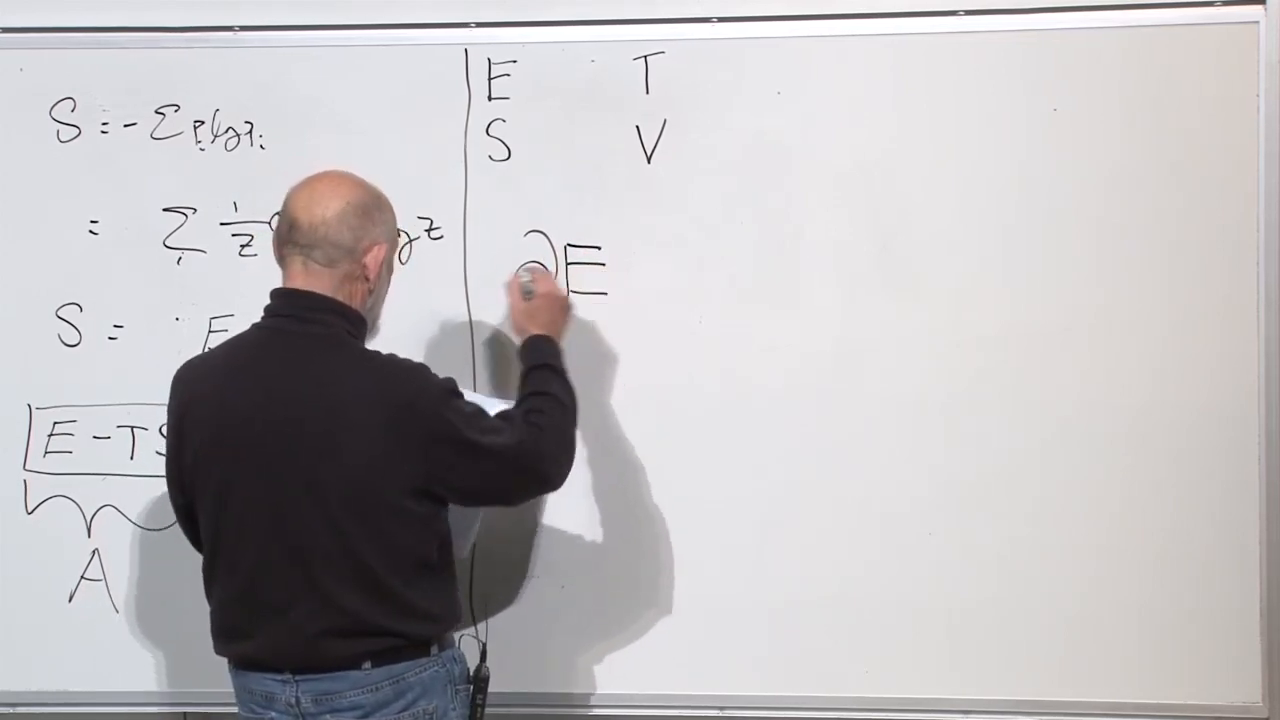
\includegraphics[width=0.90\textwidth]{lecture_05_figure_03.png}\caption{\(A=E-TS=-T\log Z\)}\lectureframe{00:16:50}\end{figure}

\section{제어변수와 그에 대한 응답}

제어변수란 실험자가 외부에서 바꿀 수 있는 거시적 물리량이다. 피스톤을 움직이면 분자 하나하나를 조작하지 않고도 부피를 바꿀 수 있다. 전기장과 자기장을 가하는 것도 다른 예다. 더 일반적인 앙상블에서는 입자 수도 변할 수 있게 둘 수 있다.

열역학 변수는 자연스럽게 켤레쌍을 이룬다. 여기서 부피는 제어변수이고 압력은 그에 대한 응답이다. \(V\)를 바꾸면 압력은 계가 그 변화에 대해 에너지적으로 어떻게 저항하는지 나타낸다. 뒤에서 에너지의 미분을 통해 이 짝 관계를 명확히 하겠다.

\begin{classroomqa}\audiencequestion{압력 자체를 제어변수로 볼 수 있나요?}
\lecturerresponse{외부 압력을 고정하는 실험을 설계할 수도 있습니다. 하지만 여기서 사용하는 구성에서는 피스톤 위치가 부피를 정하고 내부 압력이 응답으로 나타납니다. 압력과 부피는 켤레변수이며, 어느 쪽을 제어하는지는 앙상블과 장치에 따라 달라집니다.
\lecturetimestamp{00:19:22--00:20:01}}\end{classroomqa}

\begin{classroomqa}\audiencequestion{모든 분자가 동일하다고 가정하나요? 아니면 기체에만 적용되는 논증인가요?}
\lecturerresponse{열역학적 논증에는 그런 제한이 필요하지 않습니다. 실린더에는 여러 종의 입자, 액체, 심지어 압축 중인 고체도 담길 수 있습니다. 일반적인 압력 공식을 세운 뒤에야 이상기체 분배함수를 특수한 적용 사례로 다룹니다.
\lecturetimestamp{00:20:02--00:20:39}}\end{classroomqa}

\begin{classroomqa}\audiencequestion{외부에서 조작해 물질의 양을 바꿀 수도 있나요?}
\lecturerresponse{그렇습니다. 입자 수도 가능한 제어변수입니다. 이를 동적으로 다루면 그에 대응하는 켤레변수인 화학 퍼텐셜이 생깁니다. 오늘 계산에서는 \(N\)를 고정해 둡니다.
\lecturetimestamp{00:20:39--00:20:57}}\end{classroomqa}

\begin{classroomqa}\audiencequestion{액체 물과 수증기가 평형 상태에서 동시에 존재할 수 있나요?}
\lecturerresponse{공존 온도와 압력에서는 가능합니다. 중력 때문에 액체가 증기 아래에 놓여도 두 상은 같은 온도를 유지하며 열평형을 이룰 수 있습니다. 여기에도 같은 일반적인 통계역학 체계를 적용할 수 있습니다.
\lecturetimestamp{00:20:59--00:21:36}}\end{classroomqa}

다음 논증에서는 에너지와 엔트로피를 서로 독립적으로 조절할 수 있는 두 변수의 함수로 보자.
\begin{equation}
 E=E(T,V),
 \qquad
 S=S(T,V).
 \label{eq:sm5-dependent-functions}
\end{equation}
온도와 부피는 열역학적 상태 공간의 좌표다. 에너지와 엔트로피는 그 공간의 각 평형점에 값을 부여한다.

\section{엔트로피를 일정하게 유지하는 미분}

궁극적으로 필요한 미분은 특이하다.
\[
 \left(\frac{\partial E}{\partial V}\right)_S.
\]
\(T\)와 \(V\)가 독립 좌표이지만, 이 미분은 종속 함수 \(S(T,V)\)를 일정하게 유지하면서 \(V\)를 변화시키는 경우를 묻는다. 좌표축을 따라가는 미분이 아니라 \((T,V)\) 평면에서 곡선을 따라가는 미분이다.

\begin{classroomqa}\audiencequestion{\(T\)와 \(V\)가 독립인데 나중에 \(dT/dV\)를 어떻게 사용할 수 있나요?}
\lecturerresponse{전체 상태 공간에서는 두 변수가 독립입니다. \(S(T,V)=\mathrm{constant}\)라는 제약을 부과하면 허용되는 상태가 1차원 등고선 위에 놓입니다. 그 등고선을 따라서는 \(V\)의 함수로 \(T\)가 정해지고, 그 기울기 \(dT/dV\)가 정의됩니다.
\lecturetimestamp{01:01:18--01:02:09}}\end{classroomqa}

\begin{lemma}\(E(T,V)\)와 \(S(T,V)\)가 미분 가능하고 \((\partial S/\partial T)_V\neq0\)인 모든 점에서,
\begin{equation}
 \left(\frac{\partial E}{\partial V}\right)_S
 =
 \left(\frac{\partial E}{\partial V}\right)_T
 -
 \left(\frac{\partial E}{\partial S}\right)_V
 \left(\frac{\partial S}{\partial V}\right)_T.
 \label{eq:sm5-calculus-lemma}
\end{equation}\end{lemma}

\begin{proof}임의의 무한소 변위에 대해,
\begin{equation}
 dE=
 \left(\frac{\partial E}{\partial V}\right)_T dV
 +
 \left(\frac{\partial E}{\partial T}\right)_V dT.
 \label{eq:sm5-total-differential-e}
\end{equation}
\(V\)를 고정하면 연쇄법칙에 따라 \(S\)를 중간 변수로 사용할 수 있다.
\begin{equation}
 \left(\frac{\partial E}{\partial T}\right)_V
 =
 \left(\frac{\partial E}{\partial S}\right)_V
 \left(\frac{\partial S}{\partial T}\right)_V.
 \label{eq:sm5-chain-rule-e-s-t}
\end{equation}

이제 \(S\)가 일정한 등고선을 따라가는 변위만 고려하자. 그 등고선을 따라,
\begin{equation}
 0=dS=
 \left(\frac{\partial S}{\partial V}\right)_T dV
 +
 \left(\frac{\partial S}{\partial T}\right)_V dT.
 \label{eq:sm5-constant-entropy-differential}
\end{equation}
등고선의 기울이를 구하면 다음과 같다.
\begin{equation}
 \left(\frac{dT}{dV}\right)_S
 =
 -
 \frac{\left(\frac{\partial S}{\partial V}\right)_T}
 {\left(\frac{\partial S}{\partial T}\right)_V}.
 \label{eq:sm5-entropy-contour-slope}
\end{equation}
\eqref{eq:sm5-total-differential-e}를 \(dV\)로 나누고 \eqref{eq:sm5-chain-rule-e-s-t}를 사용한 뒤 \eqref{eq:sm5-entropy-contour-slope}를 대입하자.
\begin{align}
 \left(\frac{\partial E}{\partial V}\right)_S
 &=
 \left(\frac{\partial E}{\partial V}\right)_T
 +
 \left(\frac{\partial E}{\partial S}\right)_V
 \left(\frac{\partial S}{\partial T}\right)_V
 \left(\frac{dT}{dV}\right)_S \notag\\
 &=
 \left(\frac{\partial E}{\partial V}\right)_T
 -
 \left(\frac{\partial E}{\partial S}\right)_V
 \left(\frac{\partial S}{\partial V}\right)_T.
\end{align}
인수 \((\partial S/\partial T)_V\)가 약분되므로 결과가 증명된다.
\end{proof}

\begin{figure}[t]\centering
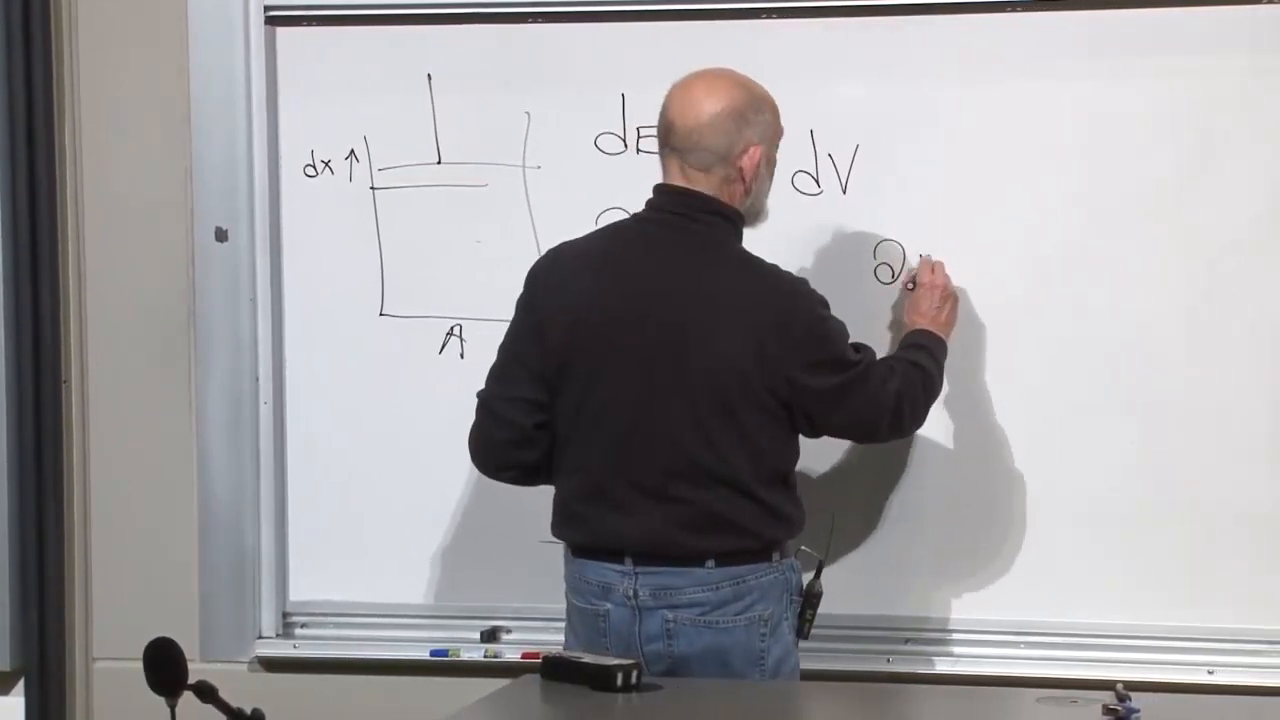
\includegraphics[width=0.90\textwidth]{lecture_05_figure_04.png}\caption{미분 보조정리를 완성하는 약분 단계에서의 일정 엔트로피 등고선 계산.}\lectureframe{00:36:10}\end{figure}

기하학적 그림은 장식이 아니다. 겉보기에는 낯선 고정 \(S\) 미분을 독립 좌표 \(T\)와 \(V\)에 대한 보통의 편미분으로 계산할 수 있는 이유를 설명해 준다. 유도 과정에서 \(\delta E/\delta V\)라고 쓰면 기호가 지정된 경로를 따라가는 작은 변화량들의 비를 나타낸다는 점을 상기하는 데 도움이 된다.

\begin{classroomqa}\audiencequestion{\(dE\)를 전개하는 것은 편미분의 통상적인 정의를 쓰는 것뿐인가요?}
\lecturerresponse{그렇습니다. 전미분에는 특별한 점이 없습니다. 추가되는 것은 나중에 \(dS=0\)인 등고선으로 제한하는 단계뿐이며, 이때 \(dT\)와 \(dV\)의 관계가 정해집니다.
\lecturetimestamp{00:29:26--00:29:32}}\end{classroomqa}

\begin{classroomqa}
\audiencequestion{상쇄가
\((\partial S/\partial T)_V\)이 0이 아니어야만 성립하나요?}
\lecturerresponse{그렇습니다. 일반적인 안정된 계에서는
\[
 \left(\frac{\partial S}{\partial T}\right)_V
 =\frac{C_V}{T}>0,
\]
따라서 나눗셈이 정당합니다. 예외적인 점에서는 별도로 주의해야 합니다. 해밀토니안이 고정된 상태에서 온도를 높이면 정준 에너지 분포가 넓어지고 엔트로피는 대개 증가하며, 온도를 낮추면 분포는 좁아집니다. 이것이 단조성 논증에서 물리적으로 올바른 방향입니다.
\lecturetimestamp{00:36:50--00:37:47}}
\end{classroomqa}

\section{피스톤이 한 일과 단열 조건}

이제 이 미분에 물리적 의미를 부여하자. 단면적이 \(\mathcal A\)인 피스톤을 생각하자. 피스톤이 바깥쪽으로 \(dx\)만큼 움직이면,
\begin{equation}
 dV=\mathcal A\,dx.
 \label{eq:sm5-piston-volume}
\end{equation}
기체는 피스톤에 \(P\mathcal A\)의 힘을 가하므로 기체가 한 일은
\begin{equation}
 \delta W_{\mathrm{by}}=P\mathcal A\,dx=P\,dV.
 \label{eq:sm5-piston-work}
\end{equation}
기체에 열이 들어오지 않으면 에너지 보존에 따라
\begin{equation}
 dE=-P\,dV.
 \label{eq:sm5-adiabatic-work}
\end{equation}
부호는 물리적 의미를 갖는다. 팽창 중에는 기체가 피스톤을 들어 올리거나 가속하고, 기체 자체의 에너지는 감소한다.

\begin{figure}[t]\centering
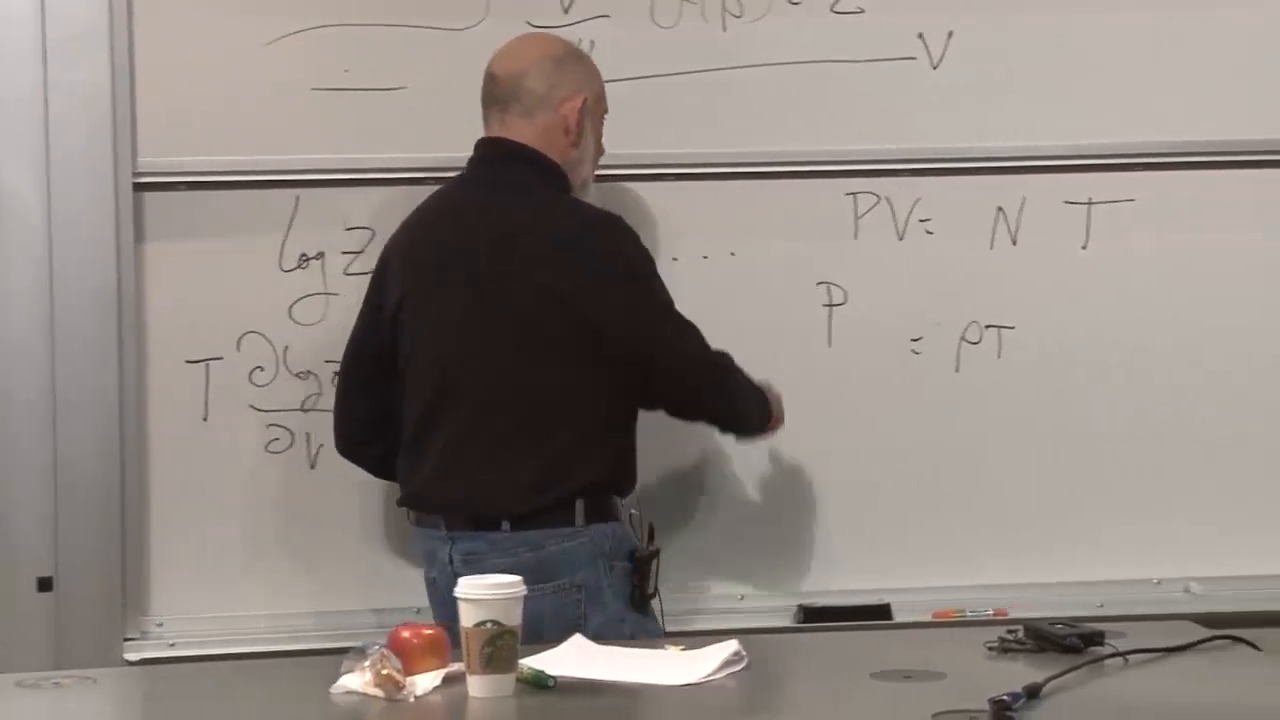
\includegraphics[width=0.90\textwidth]{lecture_05_figure_05.png}\caption{피스톤의 기하와 완성된 일의 관계 \(dE=-P\,dV\).}\lectureframe{00:43:10}\end{figure}

두 가지 조건을 반드시 만족해야 한다. 계가 평형에 임의로 가까운 상태를 유지할 만큼 피스톤이 천천히 움직여야 하고, 열이 공급되지 않도록 벽이 단열되어야 한다. 피스톤을 급히 당기면 움직이는 동안 분자가 후퇴하는 피스톤에 하나도 도달하지 못할 만큼 빠를 수 있다. 급격히 압축하면 충격파가 발생한다. 어느 과정도 평형 상태들의 연속으로 나타낼 수 없다.

\emph{단열}이라는 말은 열전달이 없다는 뜻으로 쓰이기도 하고 변화가 느리다는 뜻으로 쓰이기도 한다. 여기서 필요한 가역 과정에는 두 의미가 모두 들어간다. 변화는 준정적이며 열적으로 단열되어야 한다. 이 조건에서는 엔트로피도 일정하다.

\begin{classroomqa}\audiencequestion{단열 변화에서 엔트로피가 일정하게 유지되는 이유는 무엇인가요?}
\lecturerresponse{계를 양자역학적으로 생각해 봅시다. 다체 에너지 준위는 부피에 따라 달라집니다. \(V\)가 천천히 변하면 단열 정리에 따라 점유된 각 준위는 준위의 표지 사이에서 전이하지 않고 연속적으로 그 다음 준위로 이어집니다. 에너지 \(E_i(V)\)는 변하지만 점유 확률 \(p_i\)는 그대로 유지됩니다. \(S=-\sum_i p_i\log p_i\)는 이 확률들에 따라 정해지므로 엔트로피도 일정하게 유지됩니다. 열교환이나 비가역 운동이 있으면 이 결론은 성립하지 않습니다.
\lecturetimestamp{00:43:37--00:49:15}}\end{classroomqa}

\begin{figure}[t]\centering
\includegraphics[width=0.90\textwidth]{lecture_05_figure_06.png}\caption{점유 확률은 준위 표지를 그대로 유지하는 동안 부피에 따라 변하는 다체 에너지 준위.}\lectureframe{00:48:50}\end{figure}

이 일정 엔트로피 경로를 따라 식 \eqref{eq:sm5-adiabatic-work}을 평가하면 압력이 다음과 같이 주어진다.
\begin{equation}
 P=-\left(\frac{\partial E}{\partial V}\right)_S.
 \label{eq:sm5-pressure-fixed-entropy}
\end{equation}
이것이 압력과 부피 사이의 켤레 관계다.

\begin{classroomqa}\audiencequestion{피스톤을 빠르게 움직이면 어떻게 되나요?}
\lecturerresponse{계가 평형에서 벗어나므로 구체적인 동역학이 중요해집니다. 급격한 압축은 충격파를 일으킵니다. 이상적인 자유 팽창에서는 분자가 피스톤에 부딪히기 전에 피스톤이 후퇴할 수 있으므로 일이 이루어지지 않고, 부피가 변해도 에너지는 일정하게 유지됩니다. 이후 기체는 엔트로피가 증가한 상태로 평형에 이르도록 완화됩니다. 이런 과정은 \eqref{eq:sm5-pressure-fixed-entropy}의 단일 평형 미분으로 설명할 수 없습니다.
\lecturetimestamp{00:58:30--01:01:15}}\end{classroomqa}

\begin{classroomqa}\audiencequestion{변화가 느린지를 판별하는 정량적 조건은 무엇인가요?}
\lecturerresponse{외부 변화의 시간 척도는 관련된 내부 완화 시간보다 길어야 합니다. 기체의 경우 거시적 변화가 일어나는 동안 분자끼리 여러 차례 충돌하고 벽에도 여러 차례 부딪혀야 합니다. 정확한 시간 척도는 물질과 기하에 따라 달라지지만, 준정적 극한 자체는 일반적입니다.
\lecturetimestamp{01:02:09--01:03:20}}\end{classroomqa}

\section{단열 에너지에서 분배함수로}

물리적으로는 식 \eqref{eq:sm5-pressure-fixed-entropy}이 맞지만 계산하기 편한 형태는 아직 아니다. 정준 통계역학에서는 온도의 함수가 자연스럽게 주어진다. 볼츠만 가중치에 \(T\)가 직접 들어가기 때문이다. 미적분 보조정리를 이용하면 다루기 까다로운 고정 엔트로피 미분을 계산에 편리한 형태로 바꿀 수 있다.
\begin{align}
 P
 &=
 -\left(\frac{\partial E}{\partial V}\right)_T
 +
 \left(\frac{\partial E}{\partial S}\right)_V
 \left(\frac{\partial S}{\partial V}\right)_T.
 \label{eq:sm5-pressure-lemma-substitution}
\end{align}
부피가 고정된 상태에서 제1법칙에 따르면 \(dE=T\,dS\)이므로,
\begin{equation}
 \left(\frac{\partial E}{\partial S}\right)_V=T.
 \label{eq:sm5-e-s-temperature}
\end{equation}
따라서
\begin{equation}
 P=
 -\left(\frac{\partial E}{\partial V}\right)_T
 +
 T\left(\frac{\partial S}{\partial V}\right)_T.
 \label{eq:sm5-pressure-fixed-temperature-pieces}
\end{equation}

\begin{classroomqa}\audiencequestion{압력 공식의 마이너스 부호는 어디서 나오나요?}
\lecturerresponse{기체가 한 일에서 비롯됩니다. 단열 팽창 중에는 \(dE=-P\,dV\)입니다. 미적분 보조정리 자체에는 두 항 사이에 마이너스 부호가 있고, \(P=-(\partial E/\partial V)_S\)의 전체 마이너스 부호가 두 항의 부호를 모두 뒤집어 \eqref{eq:sm5-pressure-fixed-temperature-pieces}를 만들어 냅니다.
\lecturetimestamp{00:52:40--00:53:14}}\end{classroomqa}

두 미분 모두에서 \(T\)를 고정하므로,
\begin{align}
 P
 &=
 -\left(\frac{\partial}{\partial V}(E-TS)\right)_T \notag\\
 &=
 -\left(\frac{\partial A}{\partial V}\right)_T.
 \label{eq:sm5-pressure-free-energy}
\end{align}
마지막으로 \(A=-T\log Z\)를 대입하면,
\begin{equation}
 \boxed{
 P=
 T\left(\frac{\partial\log Z}{\partial V}\right)_T
 }.
 \label{eq:sm5-pressure-log-z}
\end{equation}

\begin{figure}[t]\centering
\includegraphics[width=0.90\textwidth]{lecture_05_figure_07.png}\caption{논증을 고정 온도에서 정리하면 다음과 같다.
\(P=-(\partial A/\partial V)_T
=T(\partial\log Z/\partial V)_T\).}\lectureframe{00:55:55}\end{figure}

식 \eqref{eq:sm5-pressure-log-z}에는 이상기체라는 가정이 전혀 들어 있지 않다. 상호작용하는 유체, 플라스마 또는 고체의 분배함수를 계산할 수 있다면 같은 미분으로 압력을 구할 수 있다. 더 일반적으로는 적절한 열역학 퍼텐셜을 미분해 모든 외부 제어변수에 대한 켤레 응답을 얻는다. 분배함수는 이러한 여러 응답을 한데 담아낸다. \(\log Z\)를 \(\beta\)에 대해 미분하면 에너지가 나오고, 부피에 대해 미분하면 압력이 나온다.

\section{이상기체 상태방정식}

이제서야 \(N\)개의 비상호작용 입자로 특수화하자. 고전적 위상공간 정규화를 유지하면,
\begin{equation}
 Z_N=
 \frac{1}{N!h^{3N}}
 \int d^{3N}q\,d^{3N}p\,
 \exp\!\left[
 -\beta\sum_{a=1}^{N}\frac{\mathbf p_a^2}{2m}
 \right].
 \label{eq:sm5-ideal-gas-partition-integral}
\end{equation}
위치 좌표가 \(3N\)개, 운동량 좌표가 \(3N\)개 있다. 해밀토니안은 위치에 의존하지 않으므로 입자마다 용기 부피에 해당하는 인수가 하나씩 생긴다.
\begin{equation}
 Z_N=
 \frac{V^N}{N!h^{3N}}I_p(\beta),
 \label{eq:sm5-ideal-gas-factorization}
\end{equation}
여기서 운동량 적분 전체인 \(I_p(\beta)\)는 \(V\)에 의존하지 않는다.

\begin{classroomqa}\audiencequestion{위치 적분은 왜 \(3N\)개이고 운동량 적분은 왜 \(3N\)개인가요?}
\lecturerresponse{입자 \(N\)개 각각에는 공간 좌표가 세 개, 그 켤레 운동량 성분이 세 개 있습니다. 위상공간의 각 절반에 있는 좌표 수는 \(3N\)개입니다. \(N\)개의 입자에 \(3N\)개의 입자를 더하는 것이 아닙니다.
\lecturetimestamp{01:04:19--01:04:28}}\end{classroomqa}

로그를 취하면 부피 의존성이 분리된다.
\begin{equation}
 \log Z_N
 =
 N\log V-\log N!-3N\log h+\log I_p(\beta).
 \label{eq:sm5-log-ideal-gas-partition}
\end{equation}
인수 \(1/N!\), \(h^{-3N}\), \(I_p(\beta)\)는 모두 부피와 무관하다. 절대 엔트로피와 다른 문제에는 중요하지만, 이 미분에는 영향을 주지 않는다. 따라서
\begin{equation}
 \left(\frac{\partial\log Z_N}{\partial V}\right)_T
 =\frac{N}{V}.
 \label{eq:sm5-log-z-volume-derivative}
\end{equation}
식 \eqref{eq:sm5-pressure-log-z}에서 곧바로 다음을 얻는다.
\begin{equation}
 P=\frac{NT}{V},
 \qquad
 \boxed{PV=NT}.
 \label{eq:sm5-ideal-gas-law}
\end{equation}

\begin{classroomqa}\audiencequestion{\(N\)는 볼츠만 분포를 유도할 때 사용한 복제계 수를 여전히 세나요?}
\lecturerresponse{아닙니다. 복제계 구성은 앞선 유도에서 계수를 세기 위한 도구였으며, 이제는 더 이상 쓰이지 않습니다. 여기서 \(N\)는 이 기체 시료 하나에 들어 있는 실제 입자 수입니다.
\lecturetimestamp{01:07:38--01:08:05}}\end{classroomqa}

수밀도를 다음과 같이 정의하면,
\begin{equation}
 \rho=\frac{N}{V}
 \label{eq:sm5-number-density}
\end{equation}
동등한 형태로 다음을 얻는다.
\begin{equation}
 P=\rho T.
 \label{eq:sm5-density-equation-of-state}
\end{equation}

\begin{classroomqa}\audiencequestion{수밀도 형태를 얻으려면 \(N\)로 나눠야 하나요, 아니면 \(V\)로 나눠야 하나요?}
\lecturerresponse{\(PV=NT\)을 \(V\)로 나누면 됩니다.
\(P=(N/V)T=\rho T\) 여기서 \(\rho\)는 질량 밀도가 아니라 수밀도입니다.
\lecturetimestamp{01:08:45--01:09:16}}\end{classroomqa}

\begin{figure}[t]\centering
\includegraphics[width=0.90\textwidth]{lecture_05_figure_08.png}\caption{\(\log Z\)의 부피 미분과 그로부터 얻는 이상기체 상태방정식 \(PV=NT\), 즉 \(P=\rho T\).}\lectureframe{01:09:25}\end{figure}

실험실 온도 \(T_K\)를 다시 쓰면,
\begin{equation}
 PV=Nk_BT_K.
 \label{eq:sm5-ideal-gas-law-laboratory}
\end{equation}
익숙한 결과가 운동론적 직관과 일치한다. 그러나 이제 그 유도는 자유 기체를 훨씬 넘어 적용되는 체계에 근거한다.

\section{두 번째 성과: 평형 요동}

압력 계산은 끝났지만, 약속한 질문 하나가 남아 있다. 분배함수에서 또 무엇을 얻을 수 있을까? 열저장고와 열접촉 중인 계를 생각해 보자. 이 계의 에너지는 고정되어 있지 않다. 에너지가 드나들기 때문에 반복해서 측정한 값은 정준 앙상블 평균을 중심으로 요동한다.

\begin{classroomqa}\audiencequestion{이제 약속했던 요동을 계산할 수 있나요?}
\lecturerresponse{그렇습니다. 남은 시간을 활용해 같은 원리를 한 번 더 보여 주겠습니다. \(Z\)의 미분에는 측정 가능한 열역학 정보가 담겨 있습니다.
\lecturetimestamp{01:10:37--01:10:50}}\end{classroomqa}

\subsection{분산과 표준편차}

\(x\)이 \(\langle x\rangle=0\)인 확률변수일 때, 분포의 폭을 나타내는 양은 \(\langle x^2\rangle\)이다. 일반적인 분포에서는 변수를 평균만큼 이동시켜 중심화한다.
\begin{equation}
 \delta x=x-\langle x\rangle.
 \label{eq:sm5-centered-variable}
\end{equation}
이 중심화된 변수의 평균은 0이며,
\begin{equation}
 \langle\delta x\rangle
 =
 \langle x\rangle-\langle x\rangle=0,
 \label{eq:sm5-centered-mean}
\end{equation}
평균제곱은 다음과 같다.
\begin{align}
 (\Delta x)^2
 &\equiv
 \left\langle\left(x-\langle x\rangle\right)^2\right\rangle \notag\\
 &=
 \langle x^2\rangle
 -2\langle x\rangle^2
 +\langle x\rangle^2 \notag\\
 &=
 \langle x^2\rangle-\langle x\rangle^2.
 \label{eq:sm5-variance}
\end{align}
이것이 분산이다. 분산의 양의 제곱근 \(\Delta x\)은 표준편차이다.

\begin{classroomqa}\audiencequestion{\(x-\langle x\rangle\)의 평균이 정확히 0인 이유는 무엇인가요?}
\lecturerresponse{평균 연산은 선형이고 \(\langle x\rangle\)는 이미 수입니다. 따라서
\(\langle x-\langle x\rangle\rangle
=\langle x\rangle-\langle x\rangle=0\)입니다.
\lecturetimestamp{01:14:02--01:14:22}}\end{classroomqa}

\begin{classroomqa}\audiencequestion{제곱 요동, 분산, 제곱평균제곱근 폭, 표준편차는 어떻게 다른가요?}
\lecturerresponse{분산은
\((\Delta x)^2=\langle x^2\rangle-\langle x\rangle^2\)입니다.
표준편차는 그 제곱근인 \(\Delta x\)입니다. 평균이 0인 변수에서는 표준편차가 제곱평균제곱근 값과도 같습니다.
\lecturetimestamp{01:16:39--01:18:38}}\end{classroomqa}

\begin{figure}[t]\centering
\includegraphics[width=0.90\textwidth]{lecture_05_figure_09.png}\caption{평균을 뺀 변수와 그 전개로 얻는 결과 \((\Delta x)^2=\langle x^2\rangle-\langle x\rangle^2\).}\lectureframe{01:17:20}\end{figure}

\subsection{분배함수에서 에너지 모멘트 구하기}

정준 앙상블에서는
\begin{align}
 \langle E\rangle
 &=
 \frac{1}{Z}\sum_i E_i e^{-\beta E_i} \notag\\
 &=
 -\frac{1}{Z}\frac{\partial Z}{\partial\beta}
 =
 -\frac{\partial\log Z}{\partial\beta}.
 \label{eq:sm5-mean-energy-from-z}
\end{align}
\(E_i\)를 인수 하나 곱하는 것은 \(\beta\)에 대한 음의 미분 한 번으로 얻는다. 두 번째 미분을 취하면 \(E_i^2\)가 나온다.
\begin{equation}
 \langle E^2\rangle
 =
 \frac{1}{Z}\sum_i E_i^2e^{-\beta E_i}
 =
 \frac{1}{Z}\frac{\partial^2 Z}{\partial\beta^2}.
 \label{eq:sm5-second-energy-moment}
\end{equation}
따라서 에너지 분산은 다음과 같다.
\begin{align}
 (\Delta E)^2
 &=
 \langle E^2\rangle-\langle E\rangle^2 \notag\\
 &=
 \frac{1}{Z}\frac{\partial^2Z}{\partial\beta^2}
 -
 \frac{1}{Z^2}
 \left(\frac{\partial Z}{\partial\beta}\right)^2 \notag\\
 &=
 \frac{\partial^2\log Z}{\partial\beta^2}
 =
 -\frac{\partial\langle E\rangle}{\partial\beta}.
 \label{eq:sm5-energy-variance-beta}
\end{align}
이번에도 복잡해 보이는 물리량이 \(\log Z\)의 미분으로 표현된다.

\begin{figure}[t]\centering
\includegraphics[width=0.90\textwidth]{lecture_05_figure_10.png}\caption{에너지 분산으로 확인되는 \(\beta\)에 대한 \(\log Z\)의 두 번째 미분.}\lectureframe{01:29:00}\end{figure}

\subsection{열용량과 요동의 크기}

강의에서 쓰는 단위에서는 \(T=1/\beta\)이므로,
\begin{equation}
 -\frac{\partial}{\partial\beta}
 =
 T^2\frac{\partial}{\partial T}.
 \label{eq:sm5-beta-temperature-derivative}
\end{equation}
부피가 고정된 상태에서 시료 전체의 열용량을 다음과 같이 정의하자.
\begin{equation}
 C_V\equiv
 \left(\frac{\partial\langle E\rangle}{\partial T}\right)_V.
 \label{eq:sm5-heat-capacity}
\end{equation}
그러면 식 \eqref{eq:sm5-energy-variance-beta}은 다음과 같이 된다.
\begin{equation}
 \boxed{(\Delta E)^2=T^2C_V}
 \qquad (k_B=1).
 \label{eq:sm5-energy-fluctuation-lecture-units}
\end{equation}
실험실 온도 \(T_K\)에서는 \(\beta=(k_BT_K)^{-1}\)이므로,
\begin{equation}
 \boxed{(\Delta E)^2=k_BT_K^2C_V}.
 \label{eq:sm5-energy-fluctuation-laboratory}
\end{equation}

\begin{figure}[t]\centering
\includegraphics[width=0.90\textwidth]{lecture_05_figure_11.png}\caption{\(\beta\) 미분을 부피 고정 열용량으로 변환하고 \(k_B\) 인수를 복원한 결과.}\lectureframe{01:31:10}\end{figure}

\begin{classroomqa}\audiencequestion{미분에서 부피를 고정할지 압력을 고정할지 명시해야 하나요?}
\lecturerresponse{그렇습니다. 이 정준 유도에서는 \(V\)를 포함해 해밀토니안의 외부 제어변수를 고정합니다. 따라서 얻는 물리량은 \(C_V\)입니다. 정압 앙상블에서는 부피와 일이 요동하므로 그에 맞는 열역학 퍼텐셜이 필요합니다. 식 \eqref{eq:sm5-energy-fluctuation-laboratory}에서 \(C_V\)를 \(C_P\)로 단순히 바꿔 쓸 수는 없습니다.
\lecturetimestamp{01:29:01--01:29:28; 01:32:50--01:33:21}}\end{classroomqa}

\begin{classroomqa}\audiencequestion{\(C_V\)는 물질 상수인가요?}
\lecturerresponse{일반적으로 그렇지 않습니다. 온도, 부피, 상, 조성에 따라 달라질 수 있습니다. 또한 여기서 \(C_V\)는 시료 전체의 열용량이므로 크기에 비례하는 양입니다. 비열을 구하려면 질량, 입자 수 또는 물질량으로 나누어야 합니다.
\lecturetimestamp{01:31:47--01:32:21; 01:33:23--01:34:55}}\end{classroomqa}

보통의 크기에 비례하는 물질에서는 \(C_V\)가 \(N\)에 비례하므로 \((\Delta E)^2\)도 \(N\)에 비례하고 \(\Delta E\)는 \(\sqrt{N}\)에 비례한다. 평균 에너지 자체는 \(N\)에 비례한다. 따라서
\begin{equation}
 \frac{\Delta E}{\langle E\rangle}\sim\frac{1}{\sqrt{N}}.
 \label{eq:sm5-relative-fluctuation-scaling}
\end{equation}
거시적 계에서는 상대 요동이 매우 작지만 미시적 시료에서는 직접 관측된다. 식 \eqref{eq:sm5-energy-fluctuation-laboratory}에 \(k_B\)가 등장한다는 것은 열역학적 물리량과 분자의 이산성 사이의 연결을 나타낸다. 다시 말해 거시적 단위와 아보가드로 수 규모의 계수를 연결한다.

압력과 요동은 이제 같은 대상에서 나왔다.
\[
 P=T\left(\frac{\partial\log Z}{\partial V}\right)_T,
 \qquad
 (\Delta E)^2=\frac{\partial^2\log Z}{\partial\beta^2}.
\]
이것이 핵심 교훈이다. 올바른 제약 조건을 찾아내면 분배함수는 확률을 정규화하는 데 그치지 않는다. 그 미분들이 계에서 측정 가능한 열역학적 성질을 체계적으로 정리해 준다.
\chapter{약한 상호작용, 비리얼 보정, 그리고 비정확 미분}

\lectureoverview{측정과 온도의 조작적 의미에서 출발해, 짧은 거리 상호작용을 약하게 켰을 때 희박 기체가 이상기체 법칙에서 어떻게 벗어나는지 살펴본다. 분배함수로 에너지와 압력에 대한 첫 상호작용 보정을 구하고, 그 유효 범위를 확인한다. 마지막 수학적 논의에서는 정확 미분, 닫힌 경로, 구체적인 이상기체 사례를 통해 상태함수와 경로에 따라 달라지는 열 및 일을 구별한다.}

\section{측정 장치가 실제로 측정하는 것}

실험실의 어떤 장치도 자연에 직접 손을 뻗어 추상적인 수학 변수의 값을 알려 주지는 않는다. 용수철저울은 늘어난 길이를 표시하고, 온도계는 액체 기둥의 높이를 표시한다. 눈에 보이는 반응과 알고자 하는 물리량 사이에 재현 가능한 관계가 성립하기 때문에, 전자를 힘의 측정이라 하고 후자를 온도의 측정이라 부른다.

그 관계가 유효한 범위는 한정되어 있다. 용수철은 탄성 한계 안에서만 후크 법칙을 따르며, 힘이 충분히 커지면 결국 변형되거나 부러진다. 더 일반적으로, 매끄러운 표시값 \(R\)이 물리량 \(X\)에 의존한다면, 선택한 작동점 근방에서는
\begin{equation}
 \Delta R \simeq
 \left.\frac{dR}{dX}\right|_{X_0}\Delta X.
 \label{eq:sm6-local-linear-response}
\end{equation}
전체 반응 곡선이 비선형이어도 표시값의 작은 변화는 목표 물리량의 작은 변화에 비례한다. 이러한 국소 선형화는 통상적인 보정의 원리다.

표시값은 교란 변수에도 의존할 수 있다. 용수철은 온도나 압력에 약하게 반응할 수 있다. 온도계의 수은 높이는 중력에 따른 방향, 유리의 성질, 또는 재료의 느린 변화에도 영향을 받을 수 있다. 측정 절차만으로 이런 의존성이 없음을 증명할 수는 없다. 대신 해당 변수를 고정하거나 필요한 정밀도에서 그 영향이 무시할 만함을 보인다.

\begin{classroomqa}
\audiencequestion{국소 중력장이나 온도계를 들고 있는 방향에 따라 눈금이 달라질 수 있나요?}
\lecturerresponse{원칙적으로는 그렇습니다. 방향이 무시할 수 없을 만큼 영향을 준다면 온도계를 수직으로 들라는 지침도 장치의 정의에 포함됩니다. 지구 표면 근처에서는 중력장이 충분히 안정적이므로, 보통 남는 변동은 무시할 만합니다.
\lecturetimestamp{00:04:08--00:05:00}}
\end{classroomqa}

\begin{classroomqa}
\audiencequestion{시간이 지나면서 노화나 화학적 변화가 보정을 서서히 바꿀 수 있나요?}
\lecturerresponse{그럴 수 있습니다. 수은과 유리는 일반적인 측정에 쓸 만큼 충분히 불활성이며, 상상하기 어려울 만큼 긴 시간에 걸친 변화는 실험과 무관합니다. 보정은 언제나 특정 장치와 범위, 절차, 지속 시간을 전제로 하는 진술입니다.
\lecturetimestamp{00:05:03--00:06:11}}
\end{classroomqa}

섭씨 온도계에서는 재현 가능한 두 기준 상태로 편리한 눈금을 정한다. 물의 어는점과 끓는점에서 액체 기둥의 높이를 각각 \(h_f\)과 \(h_b\)라 하면, 반응이 거의 선형인 범위 안에서
\begin{equation}
 T_{\mathrm C}=100\,\frac{h-h_f}{h_b-h_f}.
 \label{eq:sm6-celsius-calibration}
\end{equation}
어는점에서 \(T_{\mathrm C}=0\)로 정한 것은 관례다. 이는 열에너지가 0인 상태가 아니다. 추운 날 화씨 0도도 절대영도가 아닌 것과 같다.

\begin{figure}[t]
\centering
\includegraphics[width=0.90\textwidth]{lecture_06_figure_03.png}
선형 보정을 위해 짧은 구간을 표시한, 매끄럽지만 비선형인 온도계 반응.\caption{
}
\lectureframe{00:07:55}
\end{figure}

\section{평형과 에너지 척도로서의 온도}

온도계와 주변 매질이 열평형에 도달한 뒤에야 온도계는 주변의 온도를 측정한다. 그전의 눈금은 평형을 향해 변하고 있을 뿐이다. 실용적인 확인 방법은 간단하다. 눈금의 변화가 멈출 때까지 기다리면 된다. 이 간단한 규칙 뒤에는 대기 시간을 결정하는 물리 과정이 숨어 있다.

\begin{classroomqa}
\audiencequestion{평형화는 온도계 구 주위의 경계층에서만 일어나나요? 얼마나 기다려야 하나요?}
\lecturerresponse{에너지가 유리를 통과해 주변 매질과 교환되어야 하므로, 걸리는 시간은 온도계와 그 열전도율, 매질에 따라 달라집니다. 바로 주변 환경도 균일한 평형 상태를 대표해야 합니다. 실험에서는 눈금이 더는 변하지 않을 때 측정값을 받아들입니다.
\lecturetimestamp{00:08:45--00:10:13}}
\end{classroomqa}

온도와 밀도는 이 대기 시간에 서로 다른 역할을 한다. 매우 희박한 기체도 매우 뜨거울 수 있다. 존재하는 분자 수는 적더라도 각 분자는 큰 운동에너지를 지닐 수 있기 때문이다. 그러나 분자들이 온도계에 드물게 충돌하므로 평형화는 느릴 수 있다. 온도를 고정한 채 밀도를 100배 또는 1000배 낮춰도 분자 에너지 척도는 낮아지지 않는다. 낮아지는 것은 그 에너지가 장치에 전달되는 속도다.

\begin{classroomqa}
\audiencequestion{실내의 복사 온도가 공기의 온도와 다를 수 있나요?}
\lecturerresponse{그렇습니다. 물질과 복사가 열평형을 이룰 때에만 둘의 온도가 같습니다. 중성 공기는 조명이 켜진 실내의 광학 복사 대부분과 약하게 결합하므로, 광자 분포가 공기 온도에 해당하는 평형 흑체 복사장이 아닐 수 있습니다.
\lecturetimestamp{00:11:26--00:12:20}}
\end{classroomqa}

평형이 성립한 뒤에는 온도를 에너지 척도로 보는 것이 가장 적절하다. 계속 \(k_B=1\)인 단위를 사용하므로 \(T\) 자체의 차원은 에너지다. 단원자 이상기체에서는
\begin{equation}
 E_0=\frac{3}{2}NT.
 \label{eq:sm6-ideal-energy}
\end{equation}
분자당 열에너지는 \(T\)로 정해지지만, 그에 해당하는 속도는 여전히 분자 질량에 의존한다.

\section{약한 상호작용 켜기}

\begin{classroomqa}
\audiencequestion{어떤 조건에서 이상기체 근사가 무너지며, 그 무너짐을 수학적으로 보일 수 있나요?}
\lecturerresponse{상호작용하지 않는 기체의 해에서 출발해 작은 상호작용을 켜면 됩니다. 그 변화를 전개해 첫 보정을 계산하고 이상기체 항과 비교합니다. 보정이 더는 작지 않을 때 근사는 실패합니다.
\lecturetimestamp{00:12:25--00:14:40}}
\end{classroomqa}

이는 표준 섭동 전략이다. 문제가 \(\lambda=0\)에서 풀린다면 결합상수 \(\lambda\)를 도입하고,
\begin{equation}
 F(\lambda)=F(0)+\lambda F_1+\lambda^2F_2+\cdots,
 \label{eq:sm6-perturbative-template}
\end{equation}
각 항을 유지할 때마다 그 항이 앞선 항보다 작은지 묻는다. 여기서 기준 문제는 이상기체다. 희박한 시료, 평균 분리 거리보다 짧은 상호작용 범위, 그리고 첫 상호작용 항이 유용할 만큼 약한 퍼텐셜이 물리적 작은 양을 제공한다. 밀도가 높거나 힘의 작용 범위가 길면 각각의 충돌이 약해 보여도 근사가 무효가 될 수 있다.

분자 \(i\)의 위치와 운동량을 각각 \(x_i\in\mathbb R^3\)과 \(p_i\in\mathbb R^3\)라 하자. 질량이 \(m\)인 동일한 분자에 대해 다음과 같이 둔다.
\begin{equation}
 H(X,P)=
 \sum_{i=1}^{N}\frac{p_i^2}{2m}
 +\sum_{i<j}u\!\left(|x_i-x_j|\right),
 \label{eq:sm6-interacting-hamiltonian}
\end{equation}
여기서 \(X=(x_1,\ldots,x_N)\)이고 \(P=(p_1,\ldots,p_N)\)이다. \(i<j\)라는 제한은 자기 자신과의 쌍을 제외하고 \((i,j)\)를 한 번만 센다.
\begin{equation}
 \sum_{i<j}1=\binom{N}{2}=\frac{N(N-1)}{2}.
 \label{eq:sm6-pair-count}
\end{equation}

\begin{classroomqa}
\audiencequestion{입자 번호를 모두 사용해 각각 합을 구하면 안 되나요?}
\lecturerresponse{쌍 \((3,7)\)는 같은 물리적 쌍 \((7,3)\)와 같고, 입자는 자기 자신과 쌍을 이루지 않습니다. 합의 범위를 \(i<j\)로 제한하면 이 두 사실이 모두 반영됩니다. 질량 기호는 \(m\)로 두고 \(i,j\)는 입자를 표시하는 데 써서, \(m\)를 두 용도로 쓸 때 생길 수 있는 표기 충돌을 피합니다.
\lecturetimestamp{00:17:52--00:19:12}}
\end{classroomqa}

전체 배치 퍼텐셜을 다음과 같이 쓰자.
\begin{equation}
 U(X)=\sum_{i<j}u\!\left(|x_i-x_j|\right).
 \label{eq:sm6-total-potential}
\end{equation}
상호작용은 병진 불변이고 짧은 거리 범위를 갖는다고 가정한다. 분자 길이에 비해 \(r\)가 클 때 \(u(r)\)은 무시할 수 있을 만큼 작아진다.

\section{쌍 상호작용 세기의 적분}

첫 번째 보정에는 약한 쌍 퍼텐셜의 적분값 하나만 들어간다.
\begin{equation}
 U_0\equiv\int_{\mathbb R^3}d^3r\,u(r).
 \label{eq:sm6-u0-definition}
\end{equation}
단위는 에너지 곱하기 부피다. 상호작용의 전형적인 세기와 그 상호작용이 유효한 부피를 하나로 묶은 양이다.

\begin{figure}[t]
\centering
\includegraphics[width=0.90\textwidth]{lecture_06_figure_04.png}
\caption{단거리 쌍 퍼텐셜을 적분된 세기 \(U_0=\int d^3r\,u(r)\)로 압축한 표현}
\lectureframe{00:25:15}
\end{figure}

\(U_0\)가 왜 유용한지 알아보기 위해 한 쌍을 생각하자.
\begin{equation}
 I_2=\int_V d^3x_1\,d^3x_2\,
 u\!\left(|x_1-x_2|\right).
 \label{eq:sm6-two-particle-integral}
\end{equation}
상대좌표 \(r=x_2-x_1\)를 도입하자. 경계에서 멀리 떨어진 곳에서는 상대좌표 적분이 \(U_0\)를 주고, 쌍의 공통 위치는 용기 전체를 훑는다. 따라서
\begin{equation}
 I_2=V U_0+\text{surface corrections}.
 \label{eq:sm6-pair-integral-vu0}
\end{equation}
상호작용 범위 안에 있는 입자에서 보정이 생긴다. 이때 상대좌표의 이웃 영역 일부가 상자 밖에 놓인다. 보정의 상대적 크기는 표면적 대 부피 비율에 따라 정해지므로, 거시적 한계에서는 사라진다.

\begin{classroomqa}
\audiencequestion{\(U_0\)는 임의로 고른 한 쌍을 뜻하나요? 한 입자를 다른 입자로부터 일정한 거리에 고정하나요?}
\lecturerresponse{어떤 한 쌍에도 적용되는 공통 상호작용 법칙을 뜻합니다. 첫 번째 입자를 고정하고 두 번째 입자의 모든 상대 위치에 대해 적분합니다. 이 적분 동안 두 입자 사이 거리는 고정되지 않습니다. 가까운 상호작용 영역만 실질적으로 기여해 \(U_0\)를 만듭니다.
\lecturetimestamp{00:26:03--00:27:33}}
\end{classroomqa}

\begin{classroomqa}
\audiencequestion{왜 두 번째 위치 적분은 용기 전체 부피를 주지만 첫 번째 적분은 그렇지 않나요?}
\lecturerresponse{상대 배치를 \(U_0\)에 반영해 적분한 뒤에는 쌍 전체를 시료 안에서 평행이동할 수 있습니다. 이 공통 평행이동이 큰 인자 \(V\)를 제공합니다. 상호작용 이웃 영역은 분자 크기의 부피로 이미 \(U_0\) 안에 포함되어 있으며, 용기 부피와 같은 인자가 하나 더 생기는 것은 아닙니다.
\lecturetimestamp{00:27:48--00:29:21}}
\end{classroomqa}

\begin{classroomqa}
\audiencequestion{특히 벽 근처에서는 어느 지점을 고정하느냐에 따라 값이 달라질 수 있나요?}
\lecturerresponse{병진 불변성 때문에 벌크 값은 고정한 지점에 무관합니다. 벽 근처에서는 이웃 위치 중 일부가 허용되지 않아 적분값이 약간 달라집니다. 분자 크기의 두께를 가진 표면층만 영향을 받으므로 상자가 거시적이면 오차는 무시할 수 있습니다.
\lecturetimestamp{00:29:24--00:31:22}}
\end{classroomqa}

\begin{classroomqa}
\audiencequestion{이 결과는 두 입자의 모든 배치에 걸쳐 퍼텐셜 에너지를 적분한 값인가요? 왜 큰 부피 하나에만 비례하나요?}
\lecturerresponse{그렇습니다. \(V U_0\)에는 용기 부피 하나와 분자 크기의 상호작용 부피 하나가 들어 있으므로 단위는 에너지 곱하기 부피의 제곱입니다. 이 가운데 시료 크기에 따라 커지는 것은 첫 번째 부피뿐입니다.
\lecturetimestamp{00:31:31--00:32:04}}
\end{classroomqa}

\begin{classroomqa}
\audiencequestion{부피가 고정되었을 때 표면적을 최소화하는 구를 택하면 벌크 답이 달라지나요?}
\lecturerresponse{작은 경계 보정만 달라집니다. 일반적인 거시적 모양에서는 표면에서 분자 거리 이내에 있는 입자 수가 벌크의 입자 수에 비해 무시할 만큼 적습니다. 용기 자체의 크기가 분자 규모에 가까워질 때에만 표면이 중요해집니다.
\lecturetimestamp{00:32:04--00:33:58}}
\end{classroomqa}

\begin{classroomqa}
\audiencequestion{입자 궤적을 퍼텐셜로 바꾸면서 충돌을 생략한 건가요?}
\lecturerresponse{아닙니다. 힘은 퍼텐셜의 미분이며, 바로 그 힘이 충돌을 일으킵니다. 평형 통계역학에서는 충돌을 하나씩 따라갈 필요가 없습니다. 충돌의 효과는 에너지, 따라서 볼츠만 가중치에 담겨 있습니다.
\lecturetimestamp{00:33:59--00:35:29}}
\end{classroomqa}

\begin{classroomqa}
\audiencequestion{쌍 힘은 유지하면서 실제 삼체 상호작용은 제외하면 무엇이 빠지나요?}
\lecturerresponse{미시적 에너지에는 실제 삼체 항이 포함될 수 있고, 쌍 퍼텐셜의 고차 항도 다입자 상관을 만들어 냅니다. 그러나 희박 기체에서는 지정한 세 입자가 하나의 분자 이웃 영역에 함께 있을 가능성이 두 입자가 함께 있을 가능성보다 훨씬 낮습니다. 그러므로 쌍 효과가 첫 밀도 보정을 주고, 더 높은 클러스터는 밀도의 더 높은 거듭제곱 차수에 나타납니다.
\lecturetimestamp{00:35:29--00:38:14}}
\end{classroomqa}

\section{분배함수를 따라가는 계산}

통계적 방법의 장점이 이제 분명해진다. 해밀토니안이 주어지면 벽 근처나 충돌 중의 자세한 속도 분포를 추측할 필요가 없다. 정준 분배함수를 쓰고 그 대수를 따라가면 된다.
\begin{equation}
\begin{aligned}
 Z&=
 \frac{1}{N!h^{3N}}
 \int d^{3N}P\,d^{3N}X\\
 &\qquad{}\times e^{-\beta K(P)}e^{-\beta U(X)},\\
 K(P)&=\sum_i\frac{p_i^2}{2m}.
\end{aligned}
 \label{eq:sm6-full-partition-function}
\end{equation}
인자 \(h^{3N}\)는 고전 위상공간 측도를 무차원으로 만들고, \(N!\)는 동일 입자의 순열로 인한 중복 계산을 제거한다.

\begin{figure}[t]
\centering
\includegraphics[width=0.90\textwidth]{lecture_06_figure_05.png}
다입자 에너지와 이에 대응하는 분배함수의 운동 및 배치 인자.\caption{
}
\lectureframe{00:40:35}
\end{figure}

운동량과 위치는 분리된다. 배치 적분에 \(V^N\)를 곱했다가 나누면 이상기체 결과를 분리해 낼 수 있다.
\begin{align}
 Z
 &=\left[
 \frac{V^N}{N!h^{3N}}
 \int d^{3N}P\,e^{-\beta K(P)}
 \right] \notag\\
 &\quad\times\left[
 \frac{1}{V^N}
 \int d^{3N}X\,e^{-\beta U(X)}
 \right] \notag\\
 &\equiv Z_0\,C(\beta,V,N).
 \label{eq:sm6-z-factorization}
\end{align}
익숙한 가우스 인자는 다음과 같다.
\begin{equation}
 \int d^{3N}P\,e^{-\beta K(P)}
 =\left(\frac{2\pi m}{\beta}\right)^{3N/2}.
 \label{eq:sm6-gaussian-factor}
\end{equation}

\begin{figure}[t]
\centering
\includegraphics[width=0.90\textwidth]{lecture_06_figure_06.png}
정규화한 배치 인자에서 분리해 낸 이상기체 분배함수.\caption{
}
\lectureframe{00:43:45}
\end{figure}

인자 \(N!\)는 정규화된 비율 \(C\)이나 아래에서 사용할 특정한 고정-\(N\) 미분에는 영향을 주지 않는다. 그러나 열역학 전체에서 뺄 수 있는 인자는 아니다. 올바른 상태 수 계산과 계에 비례하는 엔트로피를 위해 필수적이다.

상호작용의 1차까지는
\begin{equation}
 e^{-\beta U(X)}
 =1-\beta U(X)+O(U^2).
 \label{eq:sm6-boltzmann-expansion}
\end{equation}
따라서
\begin{align}
 C
 &=
 1-\frac{\beta}{V^N}
 \sum_{i<j}
 \int d^{3N}X\,u(|x_i-x_j|)
 +O(U^2) \notag\\
 &=
 1-\frac{\beta}{V^N}
 \frac{N(N-1)}{2}
 V^{N-2}(V U_0)+O(U^2) \notag\\
 &=
 1-\beta\frac{N(N-1)}{2V}U_0+O(U^2).
 \label{eq:sm6-configurational-correction}
\end{align}
각 쌍은 같은 \emph{적분}을 갖지만, 순간적인 입자 간 거리나 퍼텐셜 에너지가 같은 것은 아니다. 나머지 \(N-2\)개의 위치 적분은 각각 \(V\) 인자 하나씩을 준다.

\begin{figure}[t]
\centering
\includegraphics[width=0.90\textwidth]{lecture_06_figure_07.png}
\caption{쌍의 개수 세기, 나머지 좌표들의 부피, 그리고 첫 번째 배치 보정 \(1-\beta N^2U_0/(2V)\)}
\lectureframe{00:53:40}
\end{figure}

\begin{classroomqa}
\audiencequestion{\(1\)의 선도항은 퍼텐셜이 영분리에서 사라진다고 가정하나요?}
\lecturerresponse{아닙니다. 이는 지수함수 전개의 0차 항이므로 \(u(0)\)의 값과 무관합니다. 퍼텐셜은 다음 항 \(-\beta U(X)\)에 들어갑니다.
\lecturetimestamp{00:46:19--00:46:48}}
\end{classroomqa}

\begin{classroomqa}
\audiencequestion{쌍마다 거리가 다른데 왜 모든 쌍을 같은 식으로 바꿔 써도 되나요?}
\lecturerresponse{각 위치에서의 값이 서로 같다고 하는 것이 아닙니다. 모든 항은 동일한 전체 배치 공간에 대해 적분되며, 입자 번호는 어느 쌍이냐를 구별하지 않습니다. 적분식의 형태와 값이 모두 같습니다.
\lecturetimestamp{00:50:00--00:51:07}}
\end{classroomqa}

\begin{classroomqa}
\audiencequestion{쌍의 수는 \(N(N-1)/2\)인가요, \(N(N+1)/2\)인가요?}
\lecturerresponse{\(N(N-1)/2\)입니다. 입자 하나를 고르면 서로 다른 짝은 \(N-1\)개뿐이며, 2로 나누어 순서를 뒤집은 경우를 제거합니다. 거시적인 \(N\)에 대해 \(N(N-1)\)를 \(N^2\)로 바꾸어도 상대적인 \(1/N\) 보정만 달라집니다.
\lecturetimestamp{00:48:33--00:49:56}}
\end{classroomqa}

\(\log(1-x)=-x-x^2/2-x^3/3-\cdots\)이므로, 번갈아 부호가 바뀌는 급수가 아니다. 로그의 1차 근사는
\begin{equation}
 \log Z
 =
 \log Z_0
 -\beta\frac{N(N-1)}{2V}U_0
 +O(U^2).
 \label{eq:sm6-logz-correction}
\end{equation}
\(N\)가 클 때는 유한한 \(N\) 차수의 구별이 필요하지 않으므로 \(N(N-1)\)을 \(N^2\)로 바꾸어도 된다.

\begin{remark}저밀도에서 제어 가능한 정식화에는 메이어 함수
\(f(r)=e^{-\beta u(r)}-1\)와 두 번째 비리얼 계수
\begin{equation}
 B_2(T)=-\frac{1}{2}\int d^3r\,f(r).
 \label{eq:sm6-second-virial}
\end{equation}를 사용한다. 약한 퍼텐셜에서는 \(f(r)\simeq-\beta u(r)\)이므로 \(B_2\simeq\beta U_0/2\)가 되고, 아래의 결과를 얻는다. 직접 \(e^{-\beta u}\)를 전개하는 것이 유효하지 않은 단단한 반발 코어에는 이 형식이 필요하다.
\end{remark}

\section{에너지, 압력, 그리고 보정의 의미}

\(Z\)의 로그가 유용한 이유는 그 미분값을 측정할 수 있기 때문이다. 미시적 퍼텐셜이 온도에 의존하지 않는다고 가정하면,
\begin{align}
 E
 &=-\left(\frac{\partial\log Z}{\partial\beta}\right)_{V,N} \notag\\
 &=
 \frac{3}{2}NT
 +\frac{N(N-1)}{2V}U_0+O(U^2) \notag\\
 &\simeq
 N\left(\frac{3}{2}T+\frac{1}{2}\rho U_0\right),
 \qquad
 \rho=\frac{N}{V}.
 \label{eq:sm6-energy-correction}
\end{align}
겉보기에는 계에 비례하지 않는 \(N^2\)에는 \(1/V\)이 함께 곱해져 있다. 밀도를 고정하면 \(N^2/V=N\rho\)이므로 전체 에너지는 여전히 계의 크기에 비례한다. 입자당 추가 에너지가 밀도에 비례하는 것은 선택한 분자가 가까이에 다른 분자를 만날 때에만 쌍 에너지를 얻기 때문이다.

\begin{figure}[t]
\centering
\includegraphics[width=0.90\textwidth]{lecture_06_figure_08.png}
\caption{첫 번째 상호작용 보정을 계에 비례하는 에너지로 다시 나타낸 식 \(N[3T/2+\rho U_0/2]\)}
\lectureframe{01:03:25}
\end{figure}

압력은 더 쉽게 측정할 수 있다. 앞 장의 결과를 사용하면,
\begin{equation}
 P=T\left(\frac{\partial\log Z}{\partial V}\right)_{T,N},
 \label{eq:sm6-pressure-from-z}
\end{equation}
다음과 같이 얻는다.
\begin{align}
 P
 &=
 \frac{NT}{V}
 +T\frac{\partial}{\partial V}
 \left(-\beta\frac{N(N-1)}{2V}U_0\right)
 +O(U^2) \notag\\
 &=
 \rho T+\frac{1}{2}\rho^2U_0
 +O\!\left(\frac{\rho U_0}{N},U^2\right).
 \label{eq:sm6-pressure-correction}
\end{align}

\begin{figure}[t]
\centering
\includegraphics[width=0.90\textwidth]{lecture_06_figure_09.png}
첫 번째 밀도 제곱 보정을 포함해 헬름홀츠 자유에너지의 부피 미분으로 구한 압력.\caption{
}
\lectureframe{01:09:50}
\end{figure}

\begin{classroomqa}
\audiencequestion{왜 첫 보정으로 \(\rho^2\)가 자연스럽고 다른 거듭제곱은 아닌가요?}
\lecturerresponse{이상기체 항은 작은 영역에 입자 하나가 있을 때 생기므로 \(\rho\)에 비례합니다. 상호작용에는 분자 크기의 이웃 영역에 입자 둘이 함께 있어야 하므로 그 확률은 \(\rho^2\)에 비례합니다. 인자 \(1/2\)는 쌍을 셀 때 \((i,j)\)와 \((j,i)\)를 따로 세지 않도록 하는 것과 같은 계수입니다.
\lecturetimestamp{01:24:27--01:26:00}}
\end{classroomqa}

온도를 고정한 채 \(V\)를 바꾸면서 \(\rho=N/V\)을 측정해 압력을 그래프로 그릴 수 있다. 이상기체 법칙은 선형 항이다. \(P(\rho)\)의 곡률이 첫 상호작용 보정을 드러낸다. 이 약한 퍼텐셜 근사에서는 \eqref{eq:sm6-pressure-from-z}의 인자 \(T\)가 \(\beta=1/T\)를 상쇄하므로 보정에 온도가 명시적으로 나타나지 않는다.

\begin{classroomqa}
\audiencequestion{삼체 효과를 포함해야 할 만큼 밀도가 커지는 시점은 어떻게 정하나요?}
\lecturerresponse{밀도 차수로 볼 때 다음 비리얼 항은 \(\rho^3\)에 비례하지만, 계수는 \(U_0\)만으로 추론할 수 없습니다. 쌍 상호작용의 상관된 곱과, 존재한다면 실제 삼체 힘도 기여합니다. 다음 클러스터 계수를 계산해 \(\rho^2\) 항과 비교해야 합니다. 추측한 식을 결과인 것처럼 제시해서는 안 됩니다.
\lecturetimestamp{01:10:50--01:13:38}}
\end{classroomqa}

보정의 크기가 작을 때 이상기체 항이 우세하다.
\begin{equation}
 \begin{aligned}
 \frac{1}{2}\rho^2|U_0|&\ll \rho T,\\
 |\rho U_0|&\ll T
 \qquad\text{(parametrically)}.
 \end{aligned}
 \label{eq:sm6-ideal-validity}
\end{equation}
두 번째 부등식의 양변은 모두 에너지다. \(\rho U_0\)은 입자당 상호작용 에너지 척도이고, \(T\)은 운동에너지 척도다. 보통의 희박한 실온 기체는 이 영역 안쪽에 훨씬 여유 있게 놓인다. 분자 이웃 영역이 충분히 자주 점유되어 상호작용이 열운동과 맞먹을 때에야 상당한 편차가 나타난다.

\begin{classroomqa}
\audiencequestion{이 방의 공기에 대해 이 기준을 어림할 수 있나요?}
\lecturerresponse{\(U_0\)을 분자 상호작용 에너지와 분자 부피의 곱으로 어림하고, 이를 수밀도와 곱한 결과를 \(k_BT\)와 비교하면 됩니다. 대략적인 분자 값을 대입하면 일반적인 실내 공기에서는 상호작용 척도가 훨씬 작음을 알 수 있습니다. 분자들이 서로의 상호작용 범위 안에 자주 들어갈 정도로 밀집하려면 상당한 압축이 필요합니다.
\lecturetimestamp{01:16:24--01:18:54}}
\end{classroomqa}

\begin{classroomqa}
\audiencequestion{\(U_0\)은 양수나 음수가 될 수 있나요?}
\lecturerresponse{그렇습니다. 이 근사에서 적분된 상호작용이 양수이면 순반발성이므로 압력이 \(\rho T\)보다 높아집니다. 음수이면 순인력이므로 압력이 낮아집니다. 이 부호 검사는 \eqref{eq:sm6-pressure-correction}의 물리적 타당성을 바로 확인해 줍니다.
\lecturetimestamp{01:18:56--01:20:29}}
\end{classroomqa}

\begin{figure}[t]
\centering
\includegraphics[width=0.90\textwidth]{lecture_06_figure_10.png}
\caption{반발성 및 인력 쌍 퍼텐셜의 정성적 형태와, 보정항이 \(U_0\)의 부호를 따르는 압력 공식}
\lectureframe{01:21:30}
\end{figure}

\begin{classroomqa}
\audiencequestion{정전기적 반발력, 중력에 의한 인력, 또는 실제 분자력을 이 계산에 넣을 수 있나요?}
\lecturerresponse{미시적 퍼텐셜은 원자물리학, 분자물리학 또는 양자물리학에서 주어진다. 중성 분자에는 흔히 짧은 거리에서 급격히 반발하는 코어와 더 긴 거리까지 미치는 인력성 반데르발스 꼬리가 있으며, 이를 개략적으로 12--6 퍼텐셜로 나타내기도 한다. 이런 단단한 코어에는 전체 메이어 함수 공식을 사용해야 한다. 중력은 다르다. 장거리 힘이고 공간 적분이 필요한 방식으로 수렴하지 않으므로, 여기서 사용하는 통상적인 단거리 열역학적 극한이 성립하지 않는다.
\lecturetimestamp{01:20:40--01:23:03}}
\end{classroomqa}

이 계산은 역할 분담의 유용한 예를 보여 준다. 미시물리학이 \(u(r)\)을 제공한다. 통계역학은 이 에너지로 \(Z\)를 구성하고, \(Z\)의 미분으로 벌크 관측량을 구하며, 물리적 추론으로 그 부호와 밀도 의존성, 계에 대한 비례성, 유효 범위를 점검한다. 올바른 에너지와 근사를 선택하고 나면 형식적인 계산은 기계적으로 진행된다.

\section{정확 미분과 경로 의존성}

이제 수학적 표현을 바꾸어 보자. \emph{정확 미분}에서 정확은 수치적으로 정밀하다는 뜻이 아니다. 1-형식이 실제 스칼라 함수의 미분이라는 뜻이다.

\(f(x,y)\)를 풍경 속 한 지점의 고도라고 하자. 작은 변위에 따른 고도 변화는
\begin{equation}
 df=
 \frac{\partial f}{\partial x}\,dx+
 \frac{\partial f}{\partial y}\,dy
 =f_x\,dx+f_y\,dy.
 \label{eq:sm6-total-differential}
\end{equation}
대신 다음과 같은 식만 주어졌다고 하자.
\begin{equation}
 \omega=F_x(x,y)\,dx+F_y(x,y)\,dy.
 \label{eq:sm6-one-form}
\end{equation}
\(\omega=df\)를 만족하는 스칼라 \(f\)가 존재할까? 혼합 편미분이 같아야 하므로
\begin{equation}
 \frac{\partial F_y}{\partial x}
 =
 \frac{\partial F_x}{\partial y}.
 \label{eq:sm6-exactness-condition}
\end{equation}
단일 연결 영역에서는 이 컬 조건이 충분조건이기도 하다. 그러면 성분 \((F_x,F_y)\)는 \(f\)의 기울기를 이룬다.

\begin{figure}[t]
\centering
\includegraphics[width=0.90\textwidth]{lecture_06_figure_11.png}
스칼라 함수로서의 고도, 그 미분, 그리고 정확성에 대한 혼합 편미분 조건.\caption{
}
\lectureframe{01:34:30}
\end{figure}

같은 조건은 적분으로도 해석할 수 있다. \(\omega=df\)라면,
\begin{equation}
 \int_{\gamma:1\to2}\omega=f(2)-f(1)
 \label{eq:sm6-path-independent-integral}
\end{equation}
는 경로 \(\gamma\)가 아니라 양 끝점에만 의존한다. 특히,
\begin{equation}
 \oint_\gamma\omega=0
 \label{eq:sm6-closed-loop-zero}
\end{equation}
모든 수축 가능한 닫힌 경로에 대해 성립한다.

고도는 이 성질을 갖는다. 같은 두 지점 사이를 평탄한 길로 가든 언덕을 넘어가든 고도의 순변화는 같다. 연료 소비량은 그렇지 않다. 언덕길과 평탄한 길은 일반적으로 연료를 서로 다른 양만큼 소비하고, 한 바퀴 돌아도 소모된 연료는 돌아오지 않는다. 남은 연료량은 상태를 더 자세히 기술하면 분명 잘 정의된 물리량이지만, 자동차의 위치 \((x,y)\)만의 함수는 아니다. 이동 경로의 이력이 반영된다. 피로도 마찬가지다. 언덕을 내려온다고 해서 올라가며 쌓인 피로가 대개 없어지지는 않는다.

\begin{classroomqa}
\audiencequestion{정확성은 보존력과 같은 개념인가요? 곡률과도 관련이 있나요?}
\lecturerresponse{컬이 0인 힘장은 국소적으로 보존적이며 퍼텐셜을 갖습니다. 따라서 두 개념은 밀접하게 관련되어 있습니다. 평행이동과 곡률도 닫힌 경로를 따라 생기는 변화와 국소 기하학적 자료를 연결하지만, 이는 더 넓은 주제입니다. 여기서는 기본적인 내용만 필요합니다. 통상적인 영역 조건 아래 컬이 0이면 국소적으로 경로에 무관합니다.
\lecturetimestamp{01:39:22--01:41:07}}
\end{classroomqa}

두 사례로 판정법을 구체화해 보자. 먼저 다음을 택한다.
\begin{equation}
 F_x=y,\qquad F_y=x.
 \label{eq:sm6-exact-example}
\end{equation}
두 교차 편미분은 모두 \(1\)이며, 실제로
\begin{equation}
 \omega=y\,dx+x\,dy=d(xy).
 \label{eq:sm6-exact-example-potential}
\end{equation}
이다. 이제 부호 하나를 바꾸자.
\begin{equation}
 F_x=y,\qquad F_y=-x.
 \label{eq:sm6-inexact-example}
\end{equation}
그러면
\begin{equation}
 \frac{\partial F_x}{\partial y}=1,
 \qquad
 \frac{\partial F_y}{\partial x}=-1,
 \label{eq:sm6-inexact-cross-derivatives}
\end{equation}
이므로 두 성분을 기울기로 갖는 스칼라 \(f(x,y)\)는 존재하지 않는다.

\begin{figure}[t]
\centering
\includegraphics[width=0.90\textwidth]{lecture_06_figure_12.png}
\caption{\(f=xy\)로부터 얻은 완전미분인 예와, 교차 편미분이 \(1\) 및 \(-1\)인 완전미분이 아닌 예}
\lectureframe{01:44:50}
\end{figure}

\section{열과 일은 상태함수가 아니다}

입자 수가 고정된 단순 압축성 계에서는 서로 독립인 두 평형 변수가 상태를 결정한다. \((T,V)\) 또는 \((E,V)\)를 사용할 수 있고, 기본 관계를 표현하기에는 특히 자연스러운 \((S,V)\)를 쓸 수도 있다. 따라서
\begin{equation}
 E=E(S,V),
 \end{equation}
이고, 그 정확 미분은
\begin{equation}
 dE=
 \left(\frac{\partial E}{\partial S}\right)_V dS+
 \left(\frac{\partial E}{\partial V}\right)_S dV
 =T\,dS-P\,dV.
 \label{eq:sm6-fundamental-relation}
\end{equation}

\begin{classroomqa}
\audiencequestion{단열은 느린 과정, 열적으로 절연된 과정, 가역 과정, 또는 엔트로피가 일정한 과정 중 무엇을 뜻하나요?}
\lecturerresponse{문맥에 따라 용어를 다르게 씁니다. 여기서 다루는 평형 경로에서는 변화가 준정적이고 열적으로 절연되어 있으므로 가역적이며 등엔트로피입니다. 단순히 열적으로 절연된 비가역 과정에서도 엔트로피가 생성될 수 있는 한편, 양자 단열 정리는 매개변수의 느린 변화를 강조합니다.
\lecturetimestamp{01:47:13--01:47:54}}
\end{classroomqa}

엔트로피가 고정된 팽창에서는 기체의 에너지가 \(-P\,dV\)만큼 변한다. 부피를 고정한 가역적 열 전달에서는 에너지가 \(T\,dS\)만큼 변한다. 따라서 다음과 같이 쓰면 편리하다.
\begin{equation}
 \begin{aligned}
 \delta W_{\mathrm{on}}&=-P\,dV,
 &\delta Q_{\mathrm{rev}}&=T\,dS,\\
 dE&=\delta Q_{\mathrm{rev}}+\delta W_{\mathrm{on}}.&&
 \end{aligned}
 \label{eq:sm6-first-law-increments}
\end{equation}
상태함수의 미분이 아니라 경로에 따른 증가량임을 나타내기 위해 \(d\) 대신 기호 \(\delta\)를 쓴다.

\begin{figure}[t]
\centering
\includegraphics[width=0.90\textwidth]{lecture_06_figure_13.png}
\caption{피스톤 계에 대한 열역학 제1법칙:
\(dE=-P\,dV+T\,dS\)}
\lectureframe{01:50:28}
\end{figure}

\begin{classroomqa}\audiencequestion{
\(-P\,dV\)은 기체에 가해진 일인가, 기체가 한 일인가?}\lecturerresponse{
\eqref{eq:sm6-first-law-increments}의 부호 규약에 따르면 기체에 가해진 일이다. 팽창 \(dV>0\) 동안 기체는 피스톤에 양의 일을 하므로, 기체에 가해진 일은 음수이고 기체는 에너지를 잃는다. 두 설명은 크기가 같고 부호가 반대다.
\lecturetimestamp{01:51:23--01:52:27}}
\end{classroomqa}

등식 \(\delta Q_{\mathrm{rev}}=T\,dS\)을 임의의 비가역 가열에 그대로 적용해서는 안 된다. 일반적으로는
\begin{equation}
 dS=\frac{\delta Q}{T_{\mathrm{boundary}}}+dS_{\mathrm{prod}},
 \qquad dS_{\mathrm{prod}}\ge 0.
 \label{eq:sm6-entropy-production}
\end{equation}
아래의 완전미분 논증은 준정적 평형 경로에 관한 것으로, 이때는 가역 관계가 적절하다.

\begin{classroomqa}\audiencequestion{
상태공간 논증에서 모든 경로는 평형 상태들을 지난다고 가정하나요?}\lecturerresponse{
그렇다. 경로를 따라 \(P\), \(T\), \(E\), \(S\), \(V\)가 잘 정의된 상태로 유지될 만큼 충분히 천천히 조작한다. 열과 일의 경로 의존성은 계를 평형에서 크게 벗어나게 해야만 나타나는 것이 아니다.
\lecturetimestamp{01:54:30--01:54:39}}
\end{classroomqa}

열이 완전미분인지 확인하려면 \((E,V)\)를 좌표로 사용하고 열역학 제1법칙을 다음과 같이 정리한다.
\begin{equation}
 \delta Q_{\mathrm{rev}}=dE+P(E,V)\,dV.
 \label{eq:sm6-heat-one-form}
\end{equation}
\(Q(E,V)\)라는 상태 함수가 있어서 \(dQ=\delta Q_{\mathrm{rev}}\)라면, 그 편미분은 다음과 같아야 한다.
\begin{equation}
 \left(\frac{\partial Q}{\partial E}\right)_V=1,
 \qquad
 \left(\frac{\partial Q}{\partial V}\right)_E=P.
 \label{eq:sm6-hypothetical-heat-derivatives}
\end{equation}
혼합 편미분이 같아야 하므로 다음 조건이 필요하다.
\begin{equation}
 \begin{aligned}
 \frac{\partial}{\partial V}
 \left(\frac{\partial Q}{\partial E}\right)_V
 &=\frac{\partial}{\partial E}
 \left(\frac{\partial Q}{\partial V}\right)_E,\\
 0&=\left(\frac{\partial P}{\partial E}\right)_V.
 \end{aligned}
 \label{eq:sm6-heat-exactness-requirement}
\end{equation}

\begin{classroomqa}\audiencequestion{
이는 \(F_x\,dx+F_y\,dy\)에 사용하는 컬 테스트와 정확히 같은가요?}\lecturerresponse{
그렇다. \(dE\)와 \(dV\)의 계수는 각각 \(1\)와 \(P(E,V)\)이다. 이들의 교차 편미분은 각각 \(0\)과 \((\partial P/\partial E)_V\)이다. 열이 완전미분이 되려면 이 편미분들이 같아야 한다.
\lecturetimestamp{01:54:39--01:54:52}}
\end{classroomqa}

\begin{figure}[t]
\centering
\includegraphics[width=0.90\textwidth]{lecture_06_figure_14.png}
\caption{\(dE+P\,dV\)인 열 1-형식과 이것이 상태 함수의 미분일 경우 필요한 혼합 편미분}
\lectureframe{01:58:10}
\end{figure}

이 조건은 물리적으로도 이미 그럴듯하지 않다. 부피가 일정한 상태에서 기체에 에너지를 더하면 일반적으로 압력이 변한다. 이상기체의 관계식을 이용하면 직접 계산할 수 있다.
\begin{equation}
 PV=NT,
 \qquad
 E=\frac{3}{2}NT
 \quad\Longrightarrow\quad
 P=\frac{2E}{3V}.
 \label{eq:sm6-ideal-pressure-energy}
\end{equation}
따라서
\begin{equation}
 \left(\frac{\partial P}{\partial E}\right)_V
 =\frac{2}{3V}\ne0.
 \label{eq:sm6-heat-curl-fails}
\end{equation}
컬 테스트의 조건을 만족하지 않는다. \(\delta Q_{\mathrm{rev}}\)은 완전미분이 아니다. 같은 이유로 일의 증분 \(\delta W_{\mathrm{on}}=-P\,dV\)도 완전미분이 아니다.

\begin{figure}[t]
\centering
\includegraphics[width=0.90\textwidth]{lecture_06_figure_15.png}
\caption{이상기체 관계식을 결합해 얻은 \(P=2E/(3V)\)}
\lectureframe{02:00:00}
\end{figure}

\begin{figure}[H]
\centering
\includegraphics[width=0.90\textwidth]{lecture_06_figure_16.png}
\caption{논증의 완결: \((\partial P/\partial E)_V\ne0\)이므로 열 1-형식은 완전미분일 수 없다}
\lectureframe{02:00:35}
\end{figure}

닫힌 평형 순환 과정에서는
\begin{equation}
 \oint dE=0,
 \qquad
 \oint\delta Q_{\mathrm{rev}}
 =-\oint\delta W_{\mathrm{on}}.
 \label{eq:sm6-cycle-balance}
\end{equation}
계의 에너지는 원래 값으로 돌아오지만, 열과 일은 각각 사라질 필요가 없다. 열과 일의 값은 상태 공간에서 어떤 경로를 거치는지에 따라 달라진다. 이 때문에 순환 기관은 작동 물질이 최초의 열역학적 상태로 돌아오더라도 열을 흡수하고 순일을 외부에 전달할 수 있다.

\begin{classroomqa}\audiencequestion{
이러한 경로 의존성은 기관 효율, 히스테리시스, 기억 효과와 관련이 있나요?}\lecturerresponse{
기관의 순환 과정에서는 이 경로 의존성이 직접 작용한다. 순환 과정에서 흡수한 열은 순일의 출력에 해당하며, 상태 함수 \(E\)는 초기값으로 돌아온다. 히스테리시스와 기억 효과에도 경로 의존성이 관여하지만, 이 경우에는 추가 내부 변수나 비평형 물리가 필요한 경우가 많다. 여기서 얻은 결론은 더 제한적이며 가역 평형 경로만으로도 성립한다. 열과 일은 전달되는 양이지, 열역학적 상태에 저장되는 성질이 아니다.
\lecturetimestamp{02:02:21--02:03:17}}
\end{classroomqa}

이제 논증의 두 부분이 하나로 이어진다. 측정은 측정 장치의 제어 조건과 평형 조건을 명시해야 의미가 있다. 근사는 작은 매개변수와 근사가 실패하는 기준을 명시해야 의미가 있다. 열역학적 양은 그 미분형식이 경로 독립성 검사를 통과해야 상태 함수가 된다. 어느 경우든 엄밀한 수학은 물리적 해석을 대신하지 않는다. 그 해석이 정당화되는 범위를 정확히 알려준다.
\chapter{소리, 양자 조화진동자, 그리고 제2법칙}

\lectureoverview{제2법칙이 도달할 지점이지만, 그에 앞서 구체적인 계산 두 가지를 살펴본다. 음속을 통해 열역학적 미분량이 어떻게 관측 가능한 운동으로 나타나는지 확인한다. 이어서 조화진동자로 강성이 큰 자유도에 고전적 등분배 법칙이 적용되지 않는다는 점을 살펴보고, 양자역학이 모드를 하나씩 활성화하는 방식도 확인한다. 마지막으로 위상 공간 흐름, 거친 묘사, 혼돈, 재귀를 이용해 가역적인 미시적 동역학과 증가하는 엔트로피 사이의 겉보기 모순으로 돌아간다. 이를 통해 제2법칙은 예외 없는 역학적 금지가 아니라 압도적으로 높은 확률로 성립하는 법칙임을 밝힌다.}

\section{제2법칙에 관한 약속}

핵심 문제는 말로 표현하기는 쉽지만 설명하기는 어렵다. 뉴턴 역학 방정식은 가역적이다. 어떤 미시적 과정이 허용된다면 그 시간을 거꾸로 한 과정도 허용된다. 그런데도 제2법칙은 거시적 과정에 엔트로피가 보통 증가한다는 특징으로 규정되는 선호 방향이 있다고 말한다. 이 긴장 관계를 살펴보겠지만, 바로 시작하지는 않겠다. 먼저 통계역학이 구체적인 정보를 어떻게 산출하는지 확인한 다음, 고전물리학이 양자물리학으로 대체되도록 만든 역사적 수수께끼를 간단한 계산에서 마주하는 편이 낫다.

첫 번째 예는 수치로 답을 구하되 의도적으로 거칠게 근사한다. 희박 기체의 음속을 추정해 보자. 두 번째 예는 가정이 주어진 범위에서 정확히 계산한다. 열저장고에 놓인 조화진동자의 평균 에너지를 구한다. 이 진동자를 통해 등분배 법칙에서 양자화된 에너지 준위로, 하나의 모드에서 무한히 많은 모드로 나아간 뒤, 다입자계가 초기 상태를 잊는다는 말의 의미를 묻는 문제로 돌아온다.

\section{음속의 분자 규모}

희박 기체에 작은 과밀 영역이 있다고 생각해 보자. 분자들이 밀집된 곳에서 빠져나가면서 이 영역은 퍼져 나가므로, 그 전파 속도는 분자 속도와 비슷한 규모일 것이다. 등분배 법칙으로 분자 하나의 운동에너지를 구하면 다음과 같다.
\begin{equation}
 \frac{3}{2}k_B T
 =\frac{1}{2}m\expect{v^2},
 \qquad
 \expect{v^2}=\frac{3k_B T}{m}.
 \label{eq:sm7-molecular-speed}
\end{equation}
여기서 온도는 절대영도를 기준으로 측정하며, 실험실 단위를 쓰기 위해 \(k_B\)를 다시 포함했다. 이 논증은 규모만 추정한다. 분자의 제곱평균제곱근 속도가 집단적인 음파의 속도 자체인 것은 아니다.

좀 더 체계적으로 유도하려면 기체의 작은 요소를 생각한다. 서로 마주 보는 면에 작용하는 압력이 다르면 알짜힘이 생기며, 그 가속도는 질량 밀도에 반비례한다. 그 결과는 다음 형태를 띤다.
\begin{equation}
 c_s^2=
 \left(\frac{\partial P}{\partial \rho_m}\right)_{\cal C},
 \qquad
 \rho_m=m\rho,
 \label{eq:sm7-sound-general}
\end{equation}
여기서 \(\rho\)는 수밀도이고, 아래첨자 \({\cal C}\)는 교란이 따르는 열역학적 조건을 지정한다. 판서에서 계산한 식은 다음과 같다.
\begin{equation}
 P=\rho k_B T
 \quad\Longrightarrow\quad
 \frac{1}{m}
 \left(\frac{\partial P}{\partial\rho}\right)_T
 =\frac{k_B T}{m}.
 \label{eq:sm7-sound-isothermal}
\end{equation}
이는 등온 음속 추정식이다. 제곱한 음속은 \eqref{eq:sm7-molecular-speed}의  \(3\)배이고, 음속은 \(\sqrt{3}\)배만큼 차이가 난다.

\begin{figure}[t]
\centering
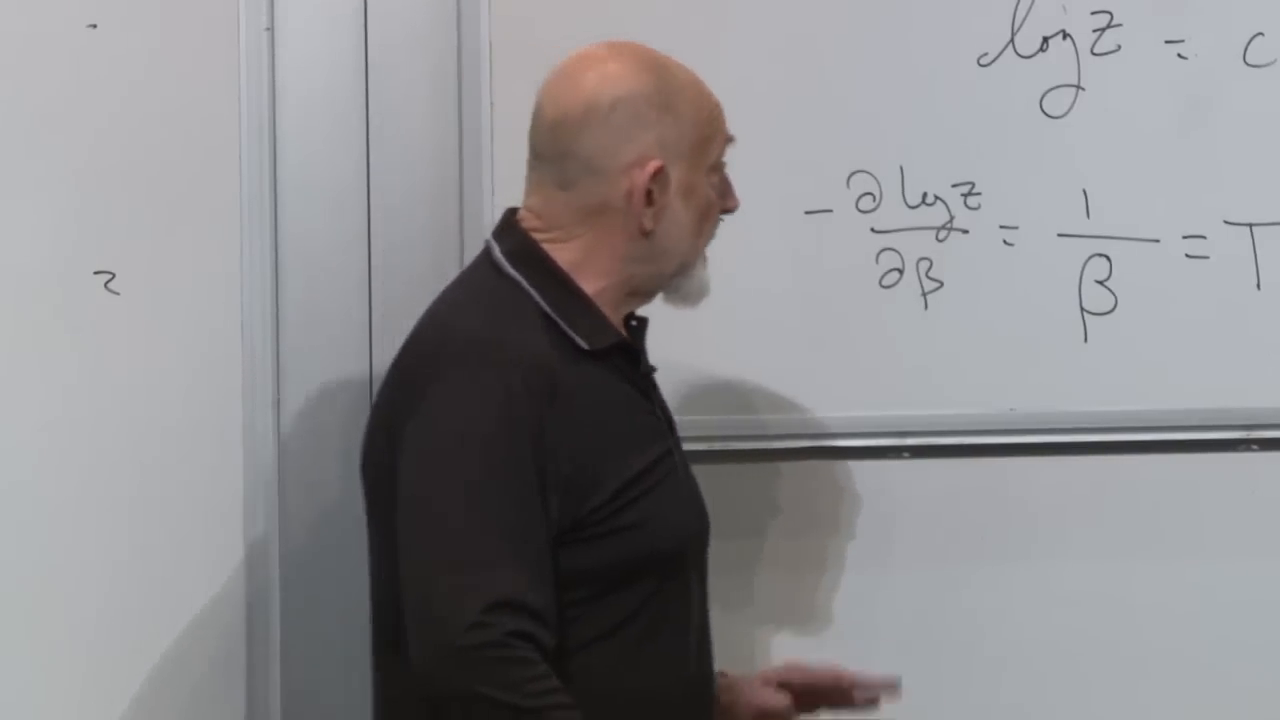
\includegraphics[width=0.90\textwidth]{lecture_07_figure_02.png}
\caption{분자 속도 추정, 압력 미분, 이상기체 대입식을 함께 나타냈다.}
\lectureframe{00:08:55}
\end{figure}

여기에는 중요한 보완이 필요하다. 진폭이 작은 음파는 보통 이웃한 기체 요소 사이에 열이 흐르는 것보다 빠르게 기체를 압축하고 팽창시킨다. 따라서 국소적인 운동은 등온이 아니라 대략 단열적이다.
\begin{equation}
 c_s^2=
 \left(\frac{\partial P}{\partial\rho_m}\right)_S.
 \label{eq:sm7-sound-adiabatic}
\end{equation}
단열지수가 \(\gamma\)인 이상기체에서는
\begin{equation}
 P\rho_m^{-\gamma}=\text{constant},
 \qquad
 c_s^2=\gamma\frac{P}{\rho_m}
       =\gamma\frac{k_B T}{m}.
 \label{eq:sm7-sound-ideal-adiabatic}
\end{equation}
실온의 이원자 기체인 공기는 \(\gamma\simeq 7/5\)이다. 그러므로 온도를 고정한 계산은 유용한 첫 추정치이고, 단열 미분이 물리적으로 적절한 보정을 제공한다.

대략적인 값으로
\begin{equation}
\begin{aligned}
 k_B&\simeq1.3\times10^{-23}\ {\rm J\,K^{-1}},
 &T&\simeq300\ {\rm K},\\
 m_{\rm air}&\simeq4\times10^{-26}\ {\rm kg}.&&
\end{aligned}
 \label{eq:sm7-air-data}
\end{equation}
분자 속도를 추정하면 약 \(500\ {\rm m\,s^{-1}}\)이다. 여기서 온도는 화씨처럼 기준점에서 벗어난 척도가 아니라 켈빈 단위의 절대온도여야 한다. 익숙한 음속은 대략 \(300\ {\rm m\,s^{-1}}\) 규모이며, 이상기체에 대한 단열식으로 계산하면 실온에서 약 \(340\ {\rm m\,s^{-1}}\)이다. 따라서 이 거친 계산으로도 올바른 물리적 규모를 얻었다.

\begin{figure}[t]
\centering
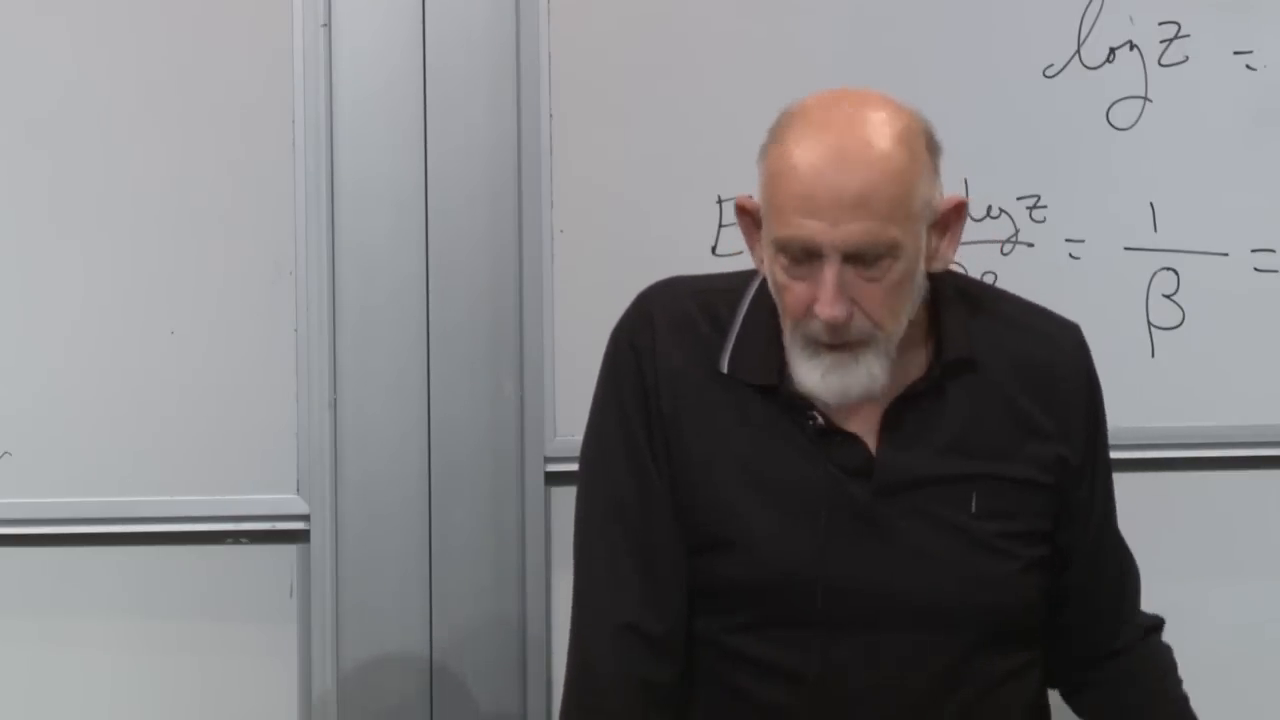
\includegraphics[width=0.90\textwidth]{lecture_07_figure_03.png}
\caption{볼츠만 상수, 양성자 질량의 약 \(30\)배인 유효 분자 질량, 그리고 \(T\simeq300\ {\rm K}\)를 사용한 실온 공기의 음속 추정.}
\lectureframe{00:10:55}
\end{figure}

미시적인 설명이 가능해지기 훨씬 전에도 압력을 밀도의 함수로 측정하면 음속을 구할 수 있었다. 통계역학적 논증은 그 결과로 얻는 거시적 속도가 개별 분자의 열속도로 정해진다는 놀라운 해석을 더해 준다.

\begin{classroomqa}
\audiencequestion{분자 질량에 중성자도 더해야 하나요? 질소에 대한 수 \(14\)는 양성자만 세나요?}
\lecturerresponse{인용된 원자량에는 이미 양성자와 중성자가 모두 포함되어 있다. 분자 질소는 원자량이 약 \(14\)인 원자 두 개로 이루어져 있으므로, 질량은 양성자 질량의 약 \(28\)배이다. 이 추정에는 \(28\)을 \(30\)로 반올림해도 충분하다.
\lecturetimestamp{00:10:58--00:11:16}}
\end{classroomqa}

\begin{classroomqa}
\audiencequestion{계수 \(3\)는 병진 방향이 세 개라는 데서 나왔는데, 음파는 한 방향으로 전파됩니다. 그러면 계수 \(3\)를 없애야 하나요?}
\lecturerresponse{이 질문은 3차원 제곱평균제곱근 분자 속도를 1차원 전파 속도와 동일시하면 안 된다는 점을 올바르게 짚는다. 도입부의 논증은 규모만 파악하려는 설명이었다. 제어된 답은 압력 미분과 파동에 적절한 열역학적 조건에서 얻는다.
\lecturetimestamp{00:11:12--00:12:00}}
\end{classroomqa}

\begin{classroomqa}
\audiencequestion{파동이 진행되는 동안 온도가 일정하다고 가정하고 미분한 건가요?}
\lecturerresponse{판서에 나온 이상기체 대입식에서는 그렇게 했다. 아주 작은 교란에서는 온도를 일정하게 두는 것이 그럴듯한 잠정 추정일 수 있다. 표준적인 보정은 일반적인 음파가 대략 단열적이라는 점을 반영하며, 이때 등온 미분 대신 \(\left(\partial P/\partial\rho_m\right)_S\)를 사용한다.
\lecturetimestamp{00:12:59--00:14:01}}
\end{classroomqa}

\begin{classroomqa}
\audiencequestion{압력 변화와 밀도 변화가 모두 작다면, 그 미분값도 작아지나요?}
\lecturerresponse{아니다. 미분은 무한소 극한에서 두 작은 변화량의 비다. \(\delta P\)와 \(\delta\rho\)는 모두 작을 수 있지만, \(\delta P/\delta\rho\)는 유한한 값으로 남아 파동 속도를 정한다.
\lecturetimestamp{00:14:03--00:14:23}}
\end{classroomqa}

\begin{classroomqa}
\audiencequestion{기체에서 액체나 고체로 갈 때처럼 기체를 압축하면 음속도 높아져야 하나요?}
\lecturerresponse{그렇다. 미분값은 고려 중인 상태에서 계산하며, \(P(\rho,T)\)가 계속 선형일 필요는 없다. 분자들이 서로 가까이 압축되면 상태방정식은 비이상적이 되고 \(\partial P/\partial\rho\)는 크게 증가할 수 있다.
\lecturetimestamp{00:14:25--00:15:13}}
\end{classroomqa}

\begin{classroomqa}
\audiencequestion{모든 압력에서 \(500\ {\rm m\,s^{-1}}\)를 사용할 수 있나요?}
\lecturerresponse{아니다. 이 값은 이상기체 방정식이 유용한 근사인 저밀도 범위에 해당한다. \(P(\rho,T)\)에 밀도의 고차항이 포함되기 시작하면 미분값과 음속은 압력과 밀도에 따라 달라진다.
\lecturetimestamp{00:15:14--00:16:29}}
\end{classroomqa}

\begin{classroomqa}
\audiencequestion{음파가 대략 분자 속도로 퍼진다는 처음의 그림도 밀도가 증가하면 성립하지 않나요?}
\lecturerresponse{그럴 가능성이 크다. 그 그림은 희박 기체에 맞춘 것이다. 밀도가 높아지면 집단적 상호작용이 점점 중요해지는데, 바로 그런 이유로 상태방정식의 미분값이 더 일반적인 설명이 된다.
\lecturetimestamp{00:16:32--00:16:53}}
\end{classroomqa}

\begin{classroomqa}
\audiencequestion{질소 분자의 질량을 \(30\)이 아니라 대략 \(28\) 양성자 질량이라고 쓴 이유는 무엇인가요?}
\lecturerresponse{이 추정에 필요한 수치 정밀도만 있으면 되므로 \(28\)를 \(30\)으로 반올림했다. 처음의 \(500\ {\rm m\,s^{-1}}\) 추정값을 \(\sqrt{3}\simeq1.7\)로 나누어도 \(300\ {\rm m\,s^{-1}}\)에 가까워지지만, 보정값을 제어된 방식으로 계산하려면 단열 미분을 써야 한다.
\lecturetimestamp{00:16:54--00:17:27}}
\end{classroomqa}

\section{열저장고 속 고전 조화진동자 하나}

이제 자유롭게 병진하는 분자 대신 조화진동자 하나를 두고 나머지는 모두 열저장고로 취급한다. 스프링에 매달린 질량이 바로 떠오르는 그림이지만, 이 모형은 훨씬 폭넓게 적용된다. 전자기 공동의 모드는 진동하고, 결정 속 원자들도 진동한다. 평형에서 조금 벗어난 거의 모든 안정한 계는 1차 근사에서 조화운동을 한다.

평형 위치에서 측정한 변위를 \(x\), 운동량을 \(p\), 질량을 \(m\), 스프링 상수를 \(\kappa\)라 하면 해밀토니안은 다음과 같다.
\begin{equation}
 H(x,p)=\frac{p^2}{2m}+\frac{\kappa x^2}{2},
 \qquad
 \omega=\sqrt{\frac{\kappa}{m}}.
 \label{eq:sm7-classical-hamiltonian}
\end{equation}
열저장고가 \(T\)를 정하며, 여기서부터는 다시 \(k_B=1\)로 두므로 \(\beta=1/T\)이다. 방 안에 둔 진동자는 약 \(300\ {\rm K}\)의 온도에 도달하고, 액체 헬륨에 담긴 진동자의 온도는 몇 켈빈에 불과하다. 태양 중심에 스프링을 놓는다면 스프링으로 남아 있지 못하겠지만, 이 예는 환경의 역할을 분명하게 보여 준다. 볼츠만 가중치는 다음처럼 인수분해된다.
\begin{equation}
 e^{-\beta H}
 =e^{-\beta p^2/(2m)}
  e^{-\beta\kappa x^2/2}.
 \label{eq:sm7-factorized-weight}
\end{equation}

\begin{figure}[t]
\centering
\includegraphics[width=0.90\textwidth]{lecture_07_figure_04.png}
\caption{스프링에 매달린 질량으로 나타낸 진동자와 운동에너지 및 퍼텐셜 에너지의 합으로 이루어진 해밀토니안.}
\lectureframe{00:20:55}
\end{figure}

자유 기체와 달리, 위치 적분은 용기의 부피만을 주지 않는다. 복원 퍼텐셜이 각 변위에 가중치를 부여한다.
\begin{equation}
 Z_{\rm cl}
 =\frac{1}{h}\int_{-\infty}^{\infty}dp
             \int_{-\infty}^{\infty}dx\,
 e^{-\beta p^2/(2m)}
 e^{-\beta\kappa x^2/2}.
 \label{eq:sm7-classical-z}
\end{equation}
인수 \(1/h\)는 1차원 고전 분배함수를 무차원으로 만든다. 판서 계산에서는 이 인수가 \(\beta\)와 무관하고 평균 에너지에 영향을 주지 않으므로 생략했다.

\begin{figure}[t]
\centering
\includegraphics[width=0.90\textwidth]{lecture_07_figure_05.png}
\caption{운동량과 변위에 관한 가우스 적분으로 분리한 고전 진동자 분배함수.}
\lectureframe{00:22:55}
\end{figure}

운동량 적분에서는 다음과 같이 치환한다.
\begin{equation}
 q=\sqrt{\frac{\beta}{2m}}\,p,
 \qquad
 dp=\sqrt{\frac{2m}{\beta}}\,dq.
 \label{eq:sm7-p-gaussian-substitution}
\end{equation}
위치 적분에서는 다음과 같이 치환한다.
\begin{equation}
 y=\sqrt{\frac{\beta\kappa}{2}}\,x,
 \qquad
 dx=\sqrt{\frac{2}{\beta\kappa}}\,dy.
 \label{eq:sm7-x-gaussian-substitution}
\end{equation}
\(\int_{-\infty}^{\infty}e^{-u^2}\,du=\sqrt{\pi}\)이므로, 판서에서 사용한 정규화 전 위상 공간 적분은 다음과 같다.
\begin{equation}
 \int dp\,dx\,e^{-\beta H}
 =\frac{2\pi}{\beta}\sqrt{\frac{m}{\kappa}}
 =\frac{2\pi}{\beta\omega}.
 \label{eq:sm7-classical-z-unnormalized}
\end{equation}
위상 공간 셀을 다시 포함하면
\begin{equation}
 Z_{\rm cl}=\frac{2\pi}{h\beta\omega}
           =\frac{1}{\beta\hbar\omega}.
 \label{eq:sm7-classical-z-normalized}
\end{equation}

에너지에는 \(\beta\)에 대한 의존성만 중요하다.
\begin{equation}
 \begin{aligned}
 \log Z_{\rm cl}&=\text{constant}-\log\beta,\\
 \expect{H}
 &=-\frac{\partial\log Z_{\rm cl}}{\partial\beta}\\
 &=\frac{1}{\beta}=T.
 \end{aligned}
 \label{eq:sm7-classical-energy}
\end{equation}

\begin{figure}[t]
\centering
\includegraphics[width=0.90\textwidth]{lecture_07_figure_06.png}
\caption{오른쪽 칠판의 고전 계산 전체 과정: 가우스 인수분해, \(Z\propto(\beta\omega)^{-1}\), 그리고 \(\expect{H}=1/\beta=T\).}
\lectureframe{00:30:15}
\end{figure}

공간 진동자가 하나이므로 \(3\) 인수는 없다. 서로 독립인 이차항이 두 개이므로 \(1/2\) 인수도 남지 않는다. 각 가우스 적분은 \(T/2\)를 기여한다.
\begin{equation}
 \expect{K}=\frac{T}{2},
 \qquad
 \expect{U}=\frac{T}{2},
 \qquad
 \expect{H}=T.
 \label{eq:sm7-equipartition-oscillator}
\end{equation}
이는 가장 유용한 형태의 등분배 법칙이다. 고전 해밀토니안의 독립적인 이차항마다 \(T/2\)가 기여한다.

답은 \(m\)와 \(\kappa\) 모두에 의존하지 않는다. 하지만 운동 자체는 이 매개변수들에 따라 달라진다.
\begin{equation}
 \expect{p^2}=mT,
 \qquad
 \expect{x^2}=\frac{T}{\kappa},
 \qquad
 \expect{\dot{x}^2}=\frac{T}{m}.
 \label{eq:sm7-classical-fluctuations}
\end{equation}
따라서 질량이 클수록 더 느리게 움직이고 스프링이 더 뻣뻣할수록 진폭이 작아지지만, 평균 에너지는 여전히 \(T\)이다. \(\kappa\)가 엄청나게 커지면 이 결과는 곤혹스러워진다. 너무 뻣뻣해서 움직이지 않는 스프링은 얼어붙은 구속조건처럼 보여야 할 텐데, 고전적 등분배 법칙은 여전히 그 에너지를 \(T\)로 준다.

\begin{classroomqa}
\audiencequestion{\(\kappa\to\infty\)일 때 분배함수는 0으로 간다. 그런데 어떻게 그 로그를 계속 사용할 수 있나요?}
\lecturerresponse{\(\kappa\)를 유한하지만 임의로 큰 값으로 두면 된다. 그것은 \(\log Z\)에 상수항으로 더해지고 \(\beta\)와 무관하므로 \(\beta\)에 대한 미분으로 여전히 \(T\)를 얻는다. 극한에서 생기는 불편함은 실제다. 고전적 계산은 내부적으로 일관되지만, 매우 뻣뻣한 진동자에 필요한 자연의 특성을 빠뜨리고 있다.
\lecturetimestamp{00:34:01--00:34:54}}
\end{classroomqa}

\begin{classroomqa}
\audiencequestion{이상기체의 분배함수에는 \(N!\)가 필요했습니다. 여기에도 비슷한 계승 인수가 있어야 하나요?}
\lecturerresponse{아니다. 여기서는 지정된 진동자 하나를 다루며, \(N\)개의 동일한 입자를 서로 바꾸어 세는 것이 아니다. 서로 독립인 모드가 여러 개라면 분배함수들을 곱한다. 비구별성 인수는 다른 셈 문제에 해당한다.
\lecturetimestamp{00:35:03--00:35:40}}
\end{classroomqa}

\section{고전적 등분배 법칙이 위기를 맞은 이유}

실제 분자는 구조가 없는 점이 아니다. 이원자 분자는 진동할 수 있는 결합을 가지므로 내부 진동자가 있다. 고전적인 방식으로 단순하게 세면 보통 온도에서도 그 모드에 추가적인 열에너지를 배정하게 된다. 의도적으로 개략화한 계산에서 진동자 하나를 활성화하면 에너지는 \(3T/2\)에서 \(5T/2\) 쪽으로 증가한다. 정확한 열용량 계산에는 회전 자유도도 포함해야 하고, 에너지와 그 온도 미분값도 구별해야 한다. 결정적인 실험 사실은 더 단순하다. 고전적 등분배 법칙의 예측과 달리, 강성이 큰 내부 모드는 저온에서 기여하지 않았다.

분자에 내부 구조가 없다고 할 수도 있겠지만, 이는 터무니없다. 아니면 고전역학에 빠진 요소가 있음을 인정해야 한다. 그 요소가 양자역학이다. 여기서는 양자역학의 아주 적은 부분만 필요하다. 조화진동자의 에너지 준위 간격이 일정하다는 사실뿐이다.

\section{양자 조화진동자}

먼저 에너지 기준점을 옮겨 들뜬 상태의 스펙트럼을 다음과 같이 쓴다.
\begin{equation}
 E_n^{\rm exc}=n\hbar\omega,
 \qquad n=0,1,2,\ldots.
 \label{eq:sm7-shifted-spectrum}
\end{equation}
이제 분배함수는 위상 공간 적분이 아니라 실제 합으로 주어진다.
\begin{align}
 Z_{\rm exc}
 &=\sum_{n=0}^{\infty}e^{-\beta n\hbar\omega} \notag\\
 &=1+x+x^2+\cdots
  =\frac{1}{1-x},
 \qquad x=e^{-\beta\hbar\omega}, \notag\\
 &=\frac{1}{1-e^{-\beta\hbar\omega}}.
 \label{eq:sm7-quantum-z}
\end{align}

\begin{figure}[t]
\centering
\includegraphics[width=0.90\textwidth]{lecture_07_figure_07.png}
\caption{등간격 에너지 준위와 양자 조화진동자 분배함수의 등비급수 계산.}
\lectureframe{00:42:05}
\end{figure}

미분하면 평균 들뜬 에너지를 얻는다.
\begin{align}
 E_{\rm exc}
 &=-\frac{\partial\log Z_{\rm exc}}{\partial\beta}
  =-\frac{1}{Z_{\rm exc}}
    \frac{\partial Z_{\rm exc}}{\partial\beta}
 \notag\\
 &=\hbar\omega\,
   \frac{e^{-\beta\hbar\omega}}
        {1-e^{-\beta\hbar\omega}}
  =\frac{\hbar\omega}{e^{\beta\hbar\omega}-1}.
 \label{eq:sm7-quantum-energy}
\end{align}

\begin{figure}[t]
\centering
\includegraphics[width=0.90\textwidth]{lecture_07_figure_08.png}
\caption{양자 분배함수를 \(\beta\)에 대해 미분해 구한 열적 들뜬 에너지.}
\lectureframe{00:46:05}
\end{figure}

\subsection{고온}

\(\beta\hbar\omega\ll1\)일 때,
\begin{equation}
 e^{-\beta\hbar\omega}
 =1-\beta\hbar\omega
  +O\!\left((\beta\hbar\omega)^2\right).
 \label{eq:sm7-high-t-expansion}
\end{equation}
\eqref{eq:sm7-quantum-energy}의 분자는 \(\hbar\omega\)에 가까워지고, 분모는 선도항에서 \(\beta\hbar\omega\)이다. 따라서
\begin{equation}
 E_{\rm exc}\simeq\frac{1}{\beta}=T.
 \label{eq:sm7-high-t-energy}
\end{equation}
열에너지 범위 안에 여러 에너지 준위 간격이 들어갈 때 양자적 결과는 고전적 등분배 법칙을 회복한다.

\subsection{저온}

\(\beta\hbar\omega\gg1\)일 때 지수항은 매우 작다.
\begin{equation}
 E_{\rm exc}
 \simeq\hbar\omega e^{-\beta\hbar\omega}.
 \label{eq:sm7-low-t-energy}
\end{equation}
진동자의 열적 들뜸은 지수적으로 억제된다. 에너지를 옮겨 쓴 관례에서는 거의 0이며, 물리적인 영점 에너지는 아래에서 다시 포함한다.

\begin{figure}[t]
\centering
\includegraphics[width=0.90\textwidth]{lecture_07_figure_09.png}
\caption{저온 전개: 첫 번째 열적 들뜸이 \(e^{-\beta\hbar\omega}\)만큼 억제된다.}
\lectureframe{00:51:55}
\end{figure}

교차는 다음 조건에서 일어난다.
\begin{equation}
 \beta\hbar\omega\sim1,
 \qquad\text{or equivalently}\qquad
 T\sim\hbar\omega.
 \label{eq:sm7-crossover}
\end{equation}
이 조건에는 직접적인 의미가 있다. 고전적 등분배 법칙은 진동자 에너지가 \(T\)라고 예측한다. 그 규모가 하나의 에너지 준위 간격보다 작아지면 양자 효과를 무시할 수 없게 된다. 따라서
\begin{equation}
\begin{aligned}
 \hbar\omega\gg T&:\quad \text{frozen and quantum},\\
 \hbar\omega\ll T&:\quad \text{active and classical}.
\end{aligned}
 \label{eq:sm7-regimes}
\end{equation}
더 뻣뻣한 스프링은 \(\omega=\sqrt{\kappa/m}\)가 더 크므로 고전적으로 거동하기 시작하려면 온도가 더 높아야 한다.

\section{물질을 가열하면 자유도가 나타난다}

저온에서 이원자 분자는 결합의 진동이 강성이 커서 얼어붙어 있으므로 점입자처럼 열적 거동을 보일 수 있다. \(T\)가 \(\hbar\omega\)을 지나 높아지면 진동 모드가 활성화된다. 회전 모드는 더 낮은 온도 규모에서 활성화될 수 있으며, 온도가 더 높아지면 다른 내부 운동이 드러나고 마침내 원자가 이온화된다. 가열은 고정된 모드 목록에 에너지를 더하기만 하는 것이 아니다. 낮은 온도에서는 보이지 않던 자유도를 드러낸다.

가상의 중첩 분자를 생각하면 요점이 더 분명해진다. 두 원자가 뻣뻣한 스프링으로 연결되어 있고, 겉으로 보이는 원자 하나도 더 뻣뻣한 스프링으로 연결된 원자 두 개로 이루어져 있다. 낮은 \(T\)에서는 두 구조 모두 점처럼 보인다. 첫 번째 임계점에서 바깥쪽 진동이 나타나고, 두 번째 임계점에서 안쪽 구조가 드러난다. 계의 복잡성은 에너지 규모에 따라 하나씩 밝혀진다.

\begin{classroomqa}
\audiencequestion{진동자가 이미 고전적 영역에 들어선 뒤에도 더 가열하면 스프링이 더 뻣뻣해지거나 진동수가 바뀌나요?}
\lecturerresponse{아니다. 스프링 상수와 진동수는 그대로다. 온도가 높아지면 전형적인 운동량과 진폭이 커져 에너지가 증가한다. 강성은 고전 법칙이 적용되기 시작하는 온도를 정할 뿐, 온도에 따라 스프링이 더 뻣뻣해지는 것은 아니다.
\lecturetimestamp{01:03:17--01:05:11}}
\end{classroomqa}

\subsection{결정과 아인슈타인의 비열}

결정에는 매우 많은 진동 모드가 있다. 고전적 등분배 법칙은 활성화된 각 진동자에 \(T\) 규모의 에너지를 배정하므로 저온 비열을 과대평가한다. 아인슈타인의 1907 모형은 결정 진동을 양자역학적으로 다루어 열에너지가 준위 간격에 이를 때까지 진동이 억제되는 이유를 보였다. 더 정밀한 고체 모형은 다양한 진동수 분포를 고려하지만, 동결 원리는 이미 아인슈타인의 계산에 담겨 있다.

\begin{classroomqa}
\audiencequestion{아인슈타인이 노벨상을 받은 업적이 이것인가요? 양자역학이 확립된 뒤에야 이 연구를 했나요?}
\lecturerresponse{아니다. 노벨상 수상 이유는 광전 효과였다. 비열 모형은 양자역학의 완전한 기초가 이해되기 훨씬 전인 1907에 발표되었다. 아인슈타인은 중요한 양자 개념을 받아들이고 발전시켰지만, 훗날 성숙한 이론의 일부 측면에는 반대했다.
\lecturetimestamp{00:58:38--01:03:16}}
\end{classroomqa}

\begin{classroomqa}
\audiencequestion{고전 통계역학은 이산 상태의 합을 위치와 운동량에 대한 겉보기에 균일한 적분으로 바꾸었습니다. 이러한 상태 세기를 정당화하는 근거는 무엇인가요?}
\lecturerresponse{궁극적인 근거는 양자역학에서 나온다. 고온 극한에서는
\[
 Z_{\rm exc}\simeq\frac{1}{\beta\hbar\omega},
\]
이는 무차원 고전 결과인 \eqref{eq:sm7-classical-z-normalized}와 정확히 일치한다. 에너지 준위 간격을 분해해 볼 수 없게 되면 위상 공간의 양자 셀이 고전적인 위상 공간 측도로 이어진다.
\lecturetimestamp{00:59:38--01:03:06}}
\end{classroomqa}

\subsection{현에는 무한히 많은 진동자가 들어 있다}

바이올린이나 기타 줄은 기본 진동, 더 높은 배음, 그리고 점점 더 짧은 파장의 정상 모드들로 분해된다. 수학적으로 진동자 모드는 무한히 많다. 고전적 등분배 법칙이 각 모드에 \(T\)의 에너지를 배정한다면 열평형에 있는 줄의 에너지는 무한대가 된다. 양자역학은 이 재앙을 막는다. 파장이 가장 짧은 모드의 진동수가 가장 높아 유한한 온도에서는 계속 얼어붙어 있고, \(T\)가 높아질수록 모드가 점차 더 많이 활성화된다. 같은 논리가 나중에 흑체 복사의 기초가 된다.

\begin{figure}[t]
\centering
\includegraphics[width=0.90\textwidth]{lecture_07_figure_10.png}
\caption{줄 위에 중첩된 여러 정상 모드. 연속적인 줄이 조화진동자 무한 개의 모음인 이유를 보여 준다.}
\lectureframe{01:09:30}
\end{figure}

\begin{classroomqa}
\audiencequestion{양자에서 고전으로의 교차를 직접 관측할 수 있나요? 가열하면 저온에서 보이던 거동이 뒤집히나요?}
\lecturerresponse{그렇다. 결정의 비열이 온도에 따라 변하는 양상을 측정하면 진동 모드의 동결과 이후의 활성화를 뚜렷하게 관측할 수 있다.
\lecturetimestamp{01:09:11--01:10:13}}
\end{classroomqa}

\begin{classroomqa}
\audiencequestion{진동자가 여러 개일 때는 각 모드마다 단일 진동자 분배함수를 반복해서 쓰나요?}
\lecturerresponse{독립 모드들의 경우
\[
\begin{aligned}
 Z_{\rm tot}&=\prod_j Z_j,&
 \log Z_{\rm tot}&=\sum_j\log Z_j,\\
 E_{\rm tot}&=\sum_j E_j.&&
\end{aligned}
\]
\(\hbar\omega_j\gg T\)인 모드는 열적 기여가 지수적으로 작고, 임계값보다 낮은 모드는 상당한 기여를 한다.
\lecturetimestamp{01:10:14--01:11:00}}
\end{classroomqa}

\begin{classroomqa}
\audiencequestion{진동자의 영점 에너지 \(\hbar\omega/2\)는 어떻게 되었나요?}
\lecturerresponse{물리적인 에너지 준위는 다음과 같다.
\[
 E_n=\left(n+\frac12\right)\hbar\omega.
\]
따라서
\[
 \begin{aligned}
 Z_{\rm phys}
 &=e^{-\beta\hbar\omega/2}Z_{\rm exc},\\
 E_{\rm phys}
 &=\frac{\hbar\omega}{2}
  +\frac{\hbar\omega}{e^{\beta\hbar\omega}-1}.
 \end{aligned}
\]
공통된 에너지 이동은 준위 확률, 엔트로피, 열용량, 열적 들뜬 에너지를 바꾸지 않지만 절대 평균 에너지를 \(\hbar\omega/2\)만큼 이동시킨다. \(Z\)의 곱셈 인자는 \(\beta\)에 의존하므로 절대 에너지를 구할 때는 버리면 안 된다.
\lecturetimestamp{01:11:08--01:11:37}}
\end{classroomqa}

\section{가역성 수수께끼로서의 제2법칙}

이제 앞서 약속한 문제로 돌아가자. 제2법칙에 따르면 일반적인 거시적 시간 변화는 비가역적이며 엔트로피는 증가하는 경향이 있다. 미시적 해밀토니안 시간 변화는 가역적이다. 가역적인 정확한 상태의 사상이 어떻게 거시적 상태에 대한 비가역 법칙을 낳을 수 있을까?

계를 고차원 위상 공간의 한 점으로 나타내자.
\[
 \Gamma=(q_1,\ldots,q_N,p_1,\ldots,p_N).
\]
우리가 아는 상태는 보통 정확한 한 점이 아니다. 부피가 \(\Omega_A\)인 유계 영역 \(A\)에서 확률밀도가 균일하다고 하자.
\begin{equation}
 f(\Gamma)=
 \begin{cases}
  1/\Omega_A,&\Gamma\in A,\\
  0,&\Gamma\notin A.
 \end{cases}
 \label{eq:sm7-uniform-blob}
\end{equation}
\(k_B=1\)인 단위계에서 미시적으로 분해된 깁스 엔트로피는 다음과 같다.
\begin{equation}
 S_{\rm fine}
 =-\int d\Gamma\,f\log f
 =\log\Omega_A.
 \label{eq:sm7-blob-entropy}
\end{equation}
영역이 작을수록 정보가 많고 엔트로피는 낮다. 따라서 부호는 분명하다. 불확실성이 커지면 점유된 영역이 넓어지고 \(\log\Omega_A\)도 증가한다.

\begin{figure}[t]
\centering
\includegraphics[width=0.90\textwidth]{lecture_07_figure_11.png}
\caption{전체 위치-운동량 위상 공간을 도식적으로 2차원으로 잘라 본 곳에 표시한 유계 확률 영역.}
\lectureframe{01:20:20}
\end{figure}

\begin{classroomqa}
\audiencequestion{계는 그려진 영역 안에 물리적으로 갇혀 있나요? 이미 평형 상태인가요?}
\lecturerresponse{아니다. 이 영역은 초기 상태에 대해 알고 있는 내용을 나타낼 뿐, 위상 공간의 벽이 아니다. 평형 분포일 필요도 없다. 예를 들어 방 한쪽 구석의 탱크에 처음 갇혀 있는 기체는 특별한 비평형 정보를 보여 준다.
\lecturetimestamp{01:14:55--01:15:24}}
\end{classroomqa}

\section{리우빌 흐름과 거친 묘사에서의 증가}

리우빌 정리에 따르면 해밀토니안 흐름은 위상 공간 부피를 보존한다. 정확한 영역은 이동하고 늘어나고 접히며 극도로 얇아질 수 있지만
\begin{equation}
 \Omega_{A(t)}=\Omega_{A(0)},
 \qquad
 S_{\rm fine}(t)=S_{\rm fine}(0).
 \label{eq:sm7-liouville}
\end{equation}
이산적인 대응물은 상태의 가역 순열이다. 처음에 주사위가 두 상태 중 하나에 있다고 알고 있다면, 일대일 시간 변화로 그 두 상태가 다른 두 상태로 바뀔 수는 있지만 가능한 상태의 수는 달라지지 않는다.

실제 묘사에는 유한한 분해능만 있다. 양자역학은 자연스러운 위상 공간 셀을 제공하며, 고전 실험도 양자 이론을 끌어들이지 않아도 측정 능력이 유한하다. 해밀토니안 흐름에 따라 영역은 길고 가느다란 뱀 모양이 될 수 있다. 이웃한 주름 사이의 간격이 분해능보다 작아지면, 구분할 수 없는 이웃 영역을 하나의 거친 셀로 대체한다. 정확한 점유 부피는 그대로지만 거친 셀들의 합집합은 커진다.
\begin{equation}
 \Omega_{\rm coarse}(t)\geq\Omega_{A(t)},
 \qquad
 S_{\rm coarse}(t)=\log\Omega_{\rm coarse}(t).
 \label{eq:sm7-coarse-entropy}
\end{equation}

\begin{figure}[t]
\centering
\includegraphics[width=0.90\textwidth]{lecture_07_figure_12.png}
\caption{유한한 분해능의 셀로 본 부피 보존 필라멘트. 정확한 검은 필라멘트의 면적은 그대로지만, 빨간색 거친 셀은 더 큰 유효 영역을 차지한다.}
\lectureframe{01:22:10}
\end{figure}

\begin{classroomqa}
\audiencequestion{거친 셀들이 겹치는데, 리우빌 정리에 어긋나지 않나요?}
\lecturerresponse{아니다. 리우빌 정리는 일대일 대응과 부피 보존을 유지하는 정확한 필라멘트에 적용된다. 겹침은 흐릿한 묘사에서 생긴다. 상태가 어느 가느다란 가닥에 있는지에 관한 정보를 버린 것이다.
\lecturetimestamp{01:21:32--01:21:50}}
\end{classroomqa}

솜에 비유하면 이해하기 쉽다. 섬유를 모두 합한 물질의 부피는 거의 그대로여도, 솜을 풀어 놓으면 각각의 섬유를 분해해 볼 수 없는 관찰자에게는 더 큰 부피를 차지하는 것처럼 보인다. 마찬가지로 위상 공간의 영역은 점점 더 미세한 촉수를 뻗고, 그 촉수는 또 더 미세한 촉수를 만든다. 고정된 유한 분해능으로는 결국 그 구조를 따라갈 수 없다.

\begin{classroomqa}
\audiencequestion{고전역학에서는 엔트로피 증가가 단지 그렇게 보일 뿐이고, 양자역학이 근본적인 분해능 한계를 부과해 그 증가를 실제로 만드는 건가요?}
\lecturerresponse{거친 묘사에 관한 논증에는 양자역학적 한계가 필요하지 않다. 엔트로피는 계와 그 묘사에서 유지되는 거시적 구분을 함께 가리킨다. 무한한 미시 정보가 있다면 미시적으로 분해된 엔트로피는 일정하다. 고정된 유한 분해능에서는 혼돈으로 생긴 필라멘트가 결국 구분되지 않게 되고 거친 묘사의 엔트로피가 증가한다.
\lecturetimestamp{01:24:04--01:25:20}}
\end{classroomqa}

\section{혼돈, 유한한 접근 가능 영역, 그리고 평형화}

상자 속 기체의 위치는 제한되어 있다. 전체 에너지가 순간적으로 한 입자에 집중되더라도, 유한한 전체 에너지에서는 운동량 역시 제한된다. 따라서 통상적인 구속 조건 아래에서 동역학적으로 접근 가능한 에너지 껍질의 측도는 유한하다.

\begin{figure}[t]
\centering
\includegraphics[width=0.90\textwidth]{lecture_07_figure_13.png}
\caption{필라멘트와 그 거친 묘사 옆에 나타낸 유계 접근 가능 위상 공간 영역.}
\lectureframe{01:28:10}
\end{figure}

혼돈계에서는 서로 가까운 초기점들이 한동안 비슷한 이력을 따르다가 서로 멀어진다. 당구에서 큐볼의 방향이 눈에 띄지 않을 만큼 조금 달라지면 그 차이가 뒤이은 충돌에 전달된다. 차이는 누적되어 마지막 상태들은 서로 무관해진다. 따라서 초기 상태의 한 영역 전체가 접근 가능한 영역을 따라 늘어나고 접힌다. 유한한 해상도에서는 넓고 거의 균일한 평형 기술에 가까워진다.

\begin{figure}[t]
\centering
\includegraphics[width=0.90\textwidth]{lecture_07_figure_14.png}
\caption{제한된 접근 가능 영역을 따라 하나의 간결한 특수 상태가 복잡한 필라멘트로 진화하는 동안, 조대화된 셀들은 훨씬 더 넓은 영역으로 퍼졌다.}
\lectureframe{01:33:10}
\end{figure}

두 가지 단서를 염두에 두어야 한다. 혼돈이라는 사실만으로 모든 궤적이 접근 가능한 모든 근방을 방문한다고 증명되는 것은 아니다. 그런 더 강한 표본화 주장을 하려면 에르고딕성이나 혼합성이 필요하다. 또한 모든 물리계가 혼돈계인 것도 아니다. 일반적인 다체 기체와 이상화된 당구는 여기서 의도하는 사례이며, 이런 계에서는 혼합성이 유용한 물리적 기대가 된다.

\section{재귀가 비가역성을 없애지는 않는다}

모든 공기 분자가 특별히 준비된 속도 패턴을 지닌 채 방 한구석에서 출발한다고 하자. 충돌이 일어나면 분자들은 빠르게 방 전체로 퍼지고, 조대화된 기술은 평형에 도달한다. 유한한 측도 보존 위상공간에서 푸앵카레 재귀 정리는 거의 모든 초기점이 출발점에 임의로 가까운 곳으로 돌아온다고 말한다. 허용오차 \(\epsilon>0\)에 대해 재귀 시간 \(t_R(\epsilon)\)은 이 정리의 가정 아래 유한하지만, 거시계에서는 터무니없이 길다. 무한히 정밀한 점으로 정확히 돌아올 필요도 없고, 일반적으로 그렇게 되리라 기대하지도 않는다.

\begin{classroomqa}
\audiencequestion{당구의 예에서 큐볼을 치면 에너지가 들어가 고립된 계의 진화라는 가정이 깨지지 않나요?}
\lecturerresponse{선택한 초기 상태는 공을 친 직후부터 시작하며, 그때의 에너지는 이미 포함되어 있다. 재귀는 그 뒤에 이어지는 고립된 이상화 당구의 동역학을 다룬다. 초기 상태에 가까운 상태로 돌아온다는 것은 선택한 허용오차 안에서 큐볼이 랙에 다가가는 것과 동등한 배치를 포함한다.
\lecturetimestamp{01:35:37--01:35:55}}
\end{classroomqa}

\begin{classroomqa}
\audiencequestion{기체가 결국 구석으로 돌아올 수 있다면, 정보가 사라진 것이고 계는 정말 가역적인가요?}
\lecturerresponse{미시적 동역학은 처음부터 끝까지 가역적이다. 미세한 상관관계를 더는 분해해 보지 않기 때문에 조대화된 엔트로피가 증가할 수 있지만, 극히 드문 요동으로 계가 특수한 초기 거시상태에 가까이 돌아올 수도 있다. 따라서 재귀와 조대화된 비가역성은 양립한다.
\lecturetimestamp{01:37:34--01:38:15}}
\end{classroomqa}

이로써 볼츠만의 핵심적인 정식화에 이른다. 논리적으로 가능한 모든 순간에 엔트로피가 증가하는 것은 아니다. 큰 계가 비평형 거시상태에 있을 때, 그 상태와 양립하는 미시적 후속 상태 가운데 훨씬 더 많은 경우가 더 특수한 상태가 아니라 더 큰 거시상태로 향한다. 엔트로피는 \emph{아마도} 증가한다. 엔트로피가 감소하는 요동과 재귀도 허용되지만, 그 확률과 시간 척도는 일상적인 거시적 경험에서 보이지 않을 만큼 작고 길다. 가역성 문제는 통계역학의 역사에서 큰 논쟁거리였으며 볼츠만에게도 큰 부담이었다. 그렇다고 이 역사적 연관성을 그의 삶에 대한 단순한 인과적 주장으로 바꾸어서는 안 된다.

\section{혼돈이 뜻하는 것}

혼돈을 좀 더 조작적으로 정의해 보자. 초기 위상점 두 개가 \(\delta\Gamma(0)\)만큼 다르다고 하자. 혼돈 방향에서는 선형화된 분리가 의미 있는 영역에서 보통 다음 관계가 성립한다.
\begin{equation}
 \lVert\delta\Gamma(t)\rVert
 \sim e^{\lambda t}\lVert\delta\Gamma(0)\rVert,
 \qquad \lambda>0,
 \label{eq:sm7-lyapunov-growth}
\end{equation}
수 \(\lambda\)를 리아푸노프 지수라고 한다. 시간 \(t\) 동안 예측하려면 초기 자료를 대략 \(e^{-\lambda t}\)에 비례하는 정밀도로 알아야 한다. 동역학 법칙의 정밀도도 중요하다. 초기 조건의 오차와 함께 모형의 오차도 증폭된다. 날씨가 익숙한 예다.

\begin{classroomqa}
\audiencequestion{\emph{대부분}의 계가 혼돈계라는 원리가 있나요, 아니면 단지 경험적 사실인가요?}
\lecturerresponse{혼돈 해밀토니안과 비혼돈 해밀토니안은 각각 무한히 많다. 게다가 \emph{대부분}이라는 말을 쓰려면 해밀토니안들의 공간에 측도를 정의해야 한다. 복잡하게 상호작용하는 계는 혼돈계인 경우가 많지만, 모든 해밀토니안을 보고 즉시 분류할 수 있는 간단하고 보편적인 검사는 없다.
\lecturetimestamp{01:39:27--01:40:49}}
\end{classroomqa}

\begin{classroomqa}
\audiencequestion{이 논의에서 \emph{혼돈적}이라는 말은 정확히 무엇을 뜻하나요?}
\lecturerresponse{가까운 위상 궤적들이 충분히 빠르게 분리되므로, 긴 시간 뒤를 예측하려면 초기 조건에 대한 지식을 지수적으로 더 정밀하게 알아야 한다. 조화진동자는 대조적인 예다. 가까운 위상점들이 함께 회전하며 계속 가까운 상태로 남는다. 정확한 이체 케플러 문제도 비혼돈계인 반면, 일반적인 삼체 문제에는 혼돈 영역이 있다.
\lecturetimestamp{01:40:50--01:43:45}}
\end{classroomqa}

\begin{classroomqa}
\audiencequestion{운동 법칙도 초기 조건과 마찬가지로 높은 정밀도로 알아야 하나요?}
\lecturerresponse{그렇다. 두 오차 원인 모두 동역학을 따라 전파되며, 혼돈적 진화는 둘 다 증폭한다.
\lecturetimestamp{01:43:46--01:43:55}}
\end{classroomqa}

이중진자는 눈에 띄는 예를 보여 준다. 보통의 진자는 적분 가능하고 예측할 수 있다. 두 번째 진자를 더하면, 거의 같은 상태에서 시작한 궤적들이 결국 서로 다르게 에너지를 주고받으며 완전히 다른 방향으로 향할 수 있다.

\begin{figure}[t]
\centering
\includegraphics[width=0.90\textwidth]{lecture_07_figure_15.png}
\caption{결정론적 혼돈의 구체적인 예인 이중진자.}
\lectureframe{01:44:40}
\end{figure}

\begin{classroomqa}
\audiencequestion{어떤 역학계는 혼돈계이고 다른 계는 그렇지 않은 이유가 무엇인가요?}
\lecturerresponse{그것은 마찰이나 실험 잡음의 결과가 아니라 해밀토니안과 그 불변 구조의 성질이다. 이를 판별하는 일은 수학적으로 어려울 수 있으며, 복잡성은 혼돈을 시사할 수는 있어도 증명하지는 않는다.
\lecturetimestamp{01:44:03--01:45:58}}
\end{classroomqa}

\begin{classroomqa}
\audiencequestion{마찰이 없는 이상적인 이중진자도 여전히 혼돈계인가요?}
\lecturerresponse{그렇다. 소산은 필요하지 않다. 정확하고 결정론적인 해밀토니안 운동도 초기 조건에 민감하게 의존할 수 있다. 무한한 정밀도의 초기 자료가 있다면 궤적을 무한히 오래 결정할 수 있지만, 정밀도가 유한하면 예측 가능 시간도 유한하다.
\lecturetimestamp{01:45:57--01:47:54}}
\end{classroomqa}

\begin{classroomqa}
\audiencequestion{혼돈은 닫힌 형태의 해가 없다는 뜻과 같은가요?}
\lecturerresponse{아니다. 혼돈계에는 대체로 전역적으로 유용한 닫힌 형태의 궤적 해가 없지만, 해석적 풀이 가능성과 민감한 의존성은 서로 다른 성질이다. 혼돈은 단지 공식을 쓸 수 없다는 사실이 아니라 궤적의 분리 양상으로 판별한다.
\lecturetimestamp{01:48:20--01:49:23}}
\end{classroomqa}

\begin{classroomqa}
\audiencequestion{혼돈이 널리 나타나는 현상은 언덕 꼭대기에서 정확히 균형을 잡는 경우와 어떻게 다른가요?}
\lecturerresponse{언덕 꼭대기는 예외적인 불안정 상태 하나다. 그 상태에서 벗어나면 가까운 궤적들이 빠르게 분리될 필요는 없다. 혼돈 영역에서는 궤도를 따라 불안정성이 전형적으로 나타나고, 가까운 위상점들이 반복해서 분리된다. 양의 리아푸노프 지수는 이러한 지속적인 증가를 나타낸다.
\lecturetimestamp{01:49:27--01:50:11}}
\end{classroomqa}

\section{미시적 운동에서 통계 법칙으로}

음속 추정은 미시적인 열운동이 거시적인 전파 규모를 어떻게 결정하는지 보여 주었고, 이어진 질문들은 어떤 열역학적 도함수를 지정해야 하는지 드러냈다. 그다음 진동자는 고전적 등분배 법칙이 어디까지 적용되고 어디서 실패하는지 보여 주었다. 양자 에너지 준위 간격은 강성이 큰 모드를 동결하고, 열용량이 온도에 따라 변하는 이유를 설명하며, 무한히 많은 고주파 모드가 무한한 열에너지를 지니는 일을 막는다.

정확한 미시 물리에서 유효한 거시적 기술로 이어지는 같은 흐름이 제2법칙의 핵심에 놓인 겉보기 모순을 해소한다. 해밀토니안 흐름은 정확한 위상공간 부피를 보존하며 가역성을 유지한다. 혼돈적 신장은 거시적 기술로는 포착할 수 없는 더 미세한 상관관계를 만들어 내므로 조대화된 점유 영역이 커진다. 재귀 정리는 드문 귀환이 금지된 일이 아님을 보장하고, 확률은 그런 귀환이 일상적인 경험을 규정하지 않는 이유를 설명한다. 제2법칙은 새로운 비가역적 미시 힘이 아니다. 자유도가 엄청나게 많은 계에서 특수한 거시적 초기 조건에 대해 진화가 압도적으로 높은 신뢰도로 향하는 통계적 방향이다.
\chapter{재귀, 비평형 질서, 그리고 이징 스핀}

\lectureoverview{방의 절반에서 방출된 기체는 평형을 향해 급속히 퍼져 나가지만, 가역역학에 따르면 충분히 긴 시간 동안 진화하면 예외적인 상태로 되돌아오는 일도 반드시 일어난다. 위상공간 부피로 그 재귀 시간을 추정하고, 재귀 현상과 설명되지 않은 우주의 저엔트로피 초기 상태를 구분한 뒤, 이로부터 생기는 난제를 바탕으로 볼츠만 뇌, 일관된 역사, 에너지 흐름으로 유지되는 생명을 논의한다.
그런 다음 자성 질서로 넘어간다. 서로 독립인 2상태 스핀은 정확히 풀 수 있는 예비 모형이다. 조합론으로 분배함수를 구하고, 자화가 쌍곡탄젠트 함수임을 보인다. 이웃한 스핀 사이의 상호작용을 도입하면 마침내 위아래-- 대칭성이 회복되고 1차원 이징 모형으로 이어진다.}

\section{언젠가 되돌아오는 방 안의 공기}

방의 왼쪽 절반에 공기가 모두 모여 있는 상태에서 시작하자. 칸막이를 이용해 이 상태를 만들 수 있다. 오른쪽 절반의 공기를 빼내고 왼쪽에 공기를 둔 다음, 벽을 없애면 된다. 기체는 방 안으로 빠르게 퍼져 열평형에 가까워진다. 엔트로피는 증가한다. 특별할 것은 없다.

이제 방을 밀폐한 채 그대로 두고 기다리자. 동전을 던져 백만 번 연속 앞면이 나오는 것은 극히 드문 기록이지만, 실험을 무한히 반복하면 결국 극히 드문 기록도 나타난다. 기체에도 같은 논리가 적용된다. 아주 먼 미래의 어느 시점에는 모든 분자가 다시 왼쪽 절반에, 또는 그와 비슷하게 특별한 영역에 놓이게 된다. 이러한 재귀를 푸앵카레 재귀라고 한다.

정확한 정리는 그림으로 설명한 것보다 조금 더 세심하게 표현해야 한다. 위상공간 부피를 보존하는 동역학이 작용하는 유한 측도의 위상공간 영역에서는 거의 모든 초기점이 시작점에 임의로 가까운 곳으로 되돌아온다. \emph{모든 분자가 방의 왼쪽 절반에 있다}와 같은 거시적 명제는 더 다루기 쉽다. 모든 분자의 좌표가 정확히 되돌아와야 하는 것이 아니라, 궤적이 유한한 거친 격자 영역에 다시 들어오기만 하면 되기 때문이다. 관건은 얼마나 오래 걸리는가이다.

\subsection{고차원 위상공간의 한 점}

\(N\)개의 고전 입자에 대해 위상공간은 \(6N\)개의 좌표로 이루어지며,
\begin{equation}
 \Gamma=(\bm x_1,\ldots,\bm x_N;\bm p_1,\ldots,\bm p_N).
 \label{eq:sm8-phase-point}
\end{equation}
위치는 방의 경계 안에 제한된다. 전체 에너지가 고정되어 있으면 운동량도 제한되는데, 입자 하나가 임의로 큰 운동량을 가지려면 그만큼 임의로 큰 에너지도 가져야 하기 때문이다. 따라서 재귀 논증의 가정 아래 허용되는 에너지 껍질의 측도는 유한하다.

위상공간의 점은 결정론적으로 움직이지만, 다체 기체에서 그 운동은 혼돈적이다. 당구공이 잇달아 충돌하는 경우처럼 가까운 궤적들은 빠르게 서로 멀어진다. 거친 격자화 뒤에는 긴 궤적이 접근 가능한 영역 전체를 헤매는 것처럼 보인다.

\begin{figure}[t]
\centering
\includegraphics[width=0.90\textwidth]{lecture_08_figure_02.png}
\caption{위상공간 영역과 그 안을 복잡하게 헤매는 궤적을 개략적으로 나타낸 그림이다. 그림은 의도적으로 저차원으로 그렸다. 실제 기체는 \(6N\)차원 공간에 놓여 있다.}
\lectureframe{00:06:41}
\end{figure}

저차원 그림을 보면 곧바로 잘못된 생각이 들기 쉽다. 특수한 상태가 그려진 직사각형의 절반을 차지한다면 기체가 그곳에서 절반의 시간을 보내리라고 생각할 수 있다. 그러나 \emph{모든 분자가 왼쪽 절반에 있다}는 조건은 위상공간 점의 좌표 하나만이 아니라 모든 위치 좌표를 제한한다.

한 공간 차원에서 움직이는 두 입자만 고려하고, 좌표를 \(x_1\)와 \(x_2\)로 두자. 이들의 구성공간은 정사각형이다. \(x_1<L/2\)라는 조건은 정사각형의 절반을 선택하고, \(x_1<L/2\)와 \(x_2<L/2\)를 모두 요구하면 정사각형의 사분의 일이 선택된다:
\begin{equation}
 P_2=\frac{1}{2}\frac{1}{2}=\frac{1}{4}.
 \label{eq:sm8-two-particle-quarter}
\end{equation}

\begin{figure}[t]
\centering
\includegraphics[width=0.90\textwidth]{lecture_08_figure_07.png}
\caption{공간 차원이 1인 입자 두 개의 경우, 작은 정사각형은 두 좌표가 모두 방에서 지정한 절반 안에 놓이는 배치를 나타낸다.}
\lectureframe{00:07:08}
\end{figure}

입자가 세 개이면 \(1/2^3\)이고, \(N\)개의 입자이면
\begin{equation}
 P_{\mathrm{half}}(N)
 =\left(\frac{1}{2}\right)^N.
 \label{eq:sm8-half-probability}
\end{equation}
핵심은 지수에 있다. 2분의 1이라는 인자는 평범하지만, 이를 거시적인 입자 수만큼 거듭제곱하면 일반적인 직관을 넘어선다.

\begin{classroomqa}
\audiencequestion{입자들이 다른 공간 방향에도 있으므로 답은 \(1/3^N\)이어야 하지 않나요?}
\lecturerresponse{부과하는 조건에 따라 다릅니다. 모든 입자가 분할 벽의 왼쪽에 있는지만 묻는다면 입자마다 하나의 이진 조건을 만족하면 되므로 답은 \(2^{-N}\)입니다. 입자의 가용 위치공간에서 독립적인 비율을 추가로 제한하면 그에 해당하는 인자가 하나 더 곱해집니다.
\lecturetimestamp{00:07:47--00:08:05}}
\end{classroomqa}

\section{위상공간 부피, 엔트로피, 재귀 시간의 척도}

같은 추정은 절반을 언급하지 않고도 쓸 수 있다. 방의 통상적인 공간 부피를 \(V\)라 하고, 모든 분자가 그 안에 있기를 요구하는 더 작은 영역을 \(v\)라 하자. 두 거시상태에서 공통인 운동량 인자를 무시하면, 이용 가능한 배치공간 부피는 다음과 같다.
\begin{equation}
 \Omega_{\mathrm{room}}\propto V^N,
 \qquad
 \Omega_{\mathrm{small}}\propto v^N.
 \label{eq:sm8-config-volumes}
\end{equation}
따라서 작은 거시상태에 머무르는 장시간 비율은 다음과 같다.
\begin{equation}
 P(v)
 =\frac{\Omega_{\mathrm{small}}}{\Omega_{\mathrm{room}}}
 =\left(\frac{v}{V}\right)^N.
 \label{eq:sm8-volume-ratio}
\end{equation}

\begin{figure}[t]
\centering
\includegraphics[width=0.90\textwidth]{lecture_08_figure_08.png}
\caption{칠판에 그린 일반적인 위상공간 부피 그림이다. 접근 가능한 영역 \(V^N\) 안에 작은 영역 \(v^N\)이 있고, 두 영역의 비는 \(v^N/V^N\)이다.}
\lectureframe{00:10:44}
\end{figure}

\(k_B=1\)인 단위계에서 엔트로피는 접근 가능한 위상공간 부피의 로그이다. 제한된 거시상태의 엔트로피가 \(S_A=\log\Omega_A\)이고 평형상태의 엔트로피가 \(S_{\rm eq}=\log\Omega_{\rm eq}\)이면,
\begin{equation}
 \begin{aligned}
 P(A)
 &=\frac{\Omega_A}{\Omega_{\rm eq}}\\
 &=\exp\!\left(S_A-S_{\rm eq}\right)\\
 &=e^{-\Delta S},\\
 \Delta S&=S_{\rm eq}-S_A.
 \end{aligned}
 \label{eq:sm8-entropy-probability}
\end{equation}
방 절반에 해당하는 상태에서는 \(\Delta S=N\log 2\)이고, \eqref{eq:sm8-entropy-probability}은 정확히 \(2^{-N}\)로 환원된다.
간략한 표현 \(P\sim e^{-S_{\rm eq}}\)은 특수 영역의 엔트로피를 고정된 기준값으로 취급할 때만 적절하다. 물리적으로 의미 있는 지수는 엔트로피 결손 \(\Delta S\)이다.

\begin{classroomqa}
\audiencequestion{이것은 전체 위상공간이 아니라 배치공간의 부피인가요?}
\lecturerresponse{이 비교에서는 그렇습니다. 운동량 분포는 같은 온도로 유지하고 위치 조건만 부과하므로, 공통인 운동량공간 인자는 약분됩니다. 일반적인 재귀 명제는 위상공간을 사용하지만, 이 특정 확률은 배치공간 부피의 비로 계산할 수 있습니다.
\lecturetimestamp{00:11:21--00:11:40}}
\end{classroomqa}

계가 미시적 상관 시간 또는 혼합 시간 \(\tau_{\rm mix}\) 뒤에 세부 위치에 관한 기억을 잃는다고 하자. 확률이 \(P(A)\)인 희귀 영역은 다음 시간 척도로 나타난다.
\begin{equation}
 \tau_{\rm rec}
 \sim \frac{\tau_{\rm mix}}{P(A)}
 \sim \tau_{\rm mix}e^{\Delta S}.
 \label{eq:sm8-recurrence-time-general}
\end{equation}
방 절반에 해당하는 조건에서는
\begin{equation}
 \tau_{\rm rec}\sim\tau_{\rm mix}2^N.
 \label{eq:sm8-recurrence-time-half}
\end{equation}
강의에서는 의도적으로 거칠게 방 크기를 추정하여 \(N\sim10^{30}\)으로 두고, 기억하기 쉬운 척도 \(\tau_{\rm rec}/\tau_{\rm mix}\sim2^{10^{30}}\)을 얻는다. 통상적인 대기 밀도에서 방 안의 분자 수는 \(10^{27}\)개에 가깝지만, \(10^{30}\)을 \(10^{27}\)으로 바꾸어도 결론은 달라지지 않는다. 재귀 시간은 여전히 우주의 나이보다 상상할 수 없을 만큼 길다.

\begin{classroomqa}
\audiencequestion{재귀 시간은 어떤 단위로 측정하나요? 초를 시간으로 바꾸거나 매우 짧은 단위를 쓰면 결론이 달라질 수 있나요?}
\lecturerresponse{차원을 지닌 앞인자는 \(\tau_{\rm mix}\)이고, 엄청나게 큰 수는 무차원 비 \(\tau_{\rm rec}/\tau_{\rm mix}\)입니다. 초를 시간으로 바꾸면 통상적인 환산 인자만큼 나누게 되는데, 이는 \(2^{10^{30}}\)에 비하면 무시할 수 있습니다. 분자들의 속도에 따라 방의 구석을 한 번 방문하는 지속 시간은 달라집니다. 여기서 추정하는 것은 그런 방문이 얼마나 드물게 시작되는가입니다. 양자 재귀 정리도 있지만, 여기서는 필요하지 않습니다.
\lecturetimestamp{00:17:24--00:19:18}}
\end{classroomqa}

\begin{classroomqa}
\audiencequestion{실험으로는 도저히 기다릴 수 없는 시간을 계산하는 목적이 무엇인가요?}
\lecturerresponse{개념적인 의미가 있습니다. 닫힌 역학계가 어떤 의미에서 가역성을 유지하는지 알려 주기 때문입니다. 계는 거의 모든 시간을 평형 근처에서 보내지만, 충분히 긴 시간 척도에서는 낮은 엔트로피를 향한 요동도 일으킵니다. 따라서 열역학 제2법칙은 특수한 초기 자료에 관한 압도적으로 높은 확률의 명제이지, 역방향 운동을 금지하는 미시적 방정식은 아닙니다.
\lecturetimestamp{00:15:12--00:16:35}}
\end{classroomqa}

\section{가역성과 특수한 초기 상태}

처음에 특수한 방 절반 영역에 의도적으로 둔다고 하자. 안쪽보다 바깥쪽의 위상공간 부피가 훨씬 크므로, 거의 모든 인접 궤적은 곧 그 영역을 벗어난다. 기체는 빠르게 퍼진 뒤, 되돌아오기까지 엄청나게 긴 시간을 기다린다. 빠른 이완과 긴 대기 시간 사이의 이러한 비대칭은 가역역학에 어긋나지 않는다.

빠져나오는 과정의 시간 역전은 그 전체 대기 시간이 아니다. 평형처럼 보이는 분자 속도들이 우연히 조율되어 기체가 방의 한쪽 절반으로 \emph{쏜살같이 모여드는} 짧고 기묘하게 정교한 과정이 시간 역전이다. 보통의 탈출이 끝난 시점에 모든 운동량의 방향을 뒤집으면 기체는 탈출 경로를 거꾸로 되짚는다. 그 특수한 유입 속도 배열이 저절로 생길 때까지 기다리는 데 긴 시간이 걸린다.

\begin{classroomqa}
\audiencequestion{시간 대칭성에 따르면 구석으로 천천히 재귀하는 데 처음 빠져나올 때만큼 오래 걸리나요?}
\lecturerresponse{아닙니다. 탈출 과정과 그 정확한 시간 역전을 비교해 보십시오. 둘 다 빠릅니다. 엄청나게 오래 걸리는 것은 평형 상태에서 역방향의 급격한 모임을 시작하게 할 정확한 유입 요동을 기다리는 일입니다. 엄청나게 긴 시간 기록을 보면, 평형에서 벗어나는 요동은 양쪽 시간 방향에서 국소적인 역사가 대칭을 이루며 일어납니다.
\lecturetimestamp{00:20:46--00:21:58}}
\end{classroomqa}

따라서 재귀 논증은 시간의 화살에 관한 설명의 일부만 제공한다. 계가 저엔트로피 영역에서 시작했다는 \emph{조건 아래} 왜 엔트로피가 보통 증가하는지를 설명한다. 하지만 초기 조건이 왜 특수했는지는 설명하지 못한다. 우주론에서 이 누락된 전제가 핵심 질문이 된다. 관측 가능한 우주는 왜 중력 위상공간에서 그토록 예외적으로 작은 영역에서 시작했는가?

\begin{classroomqa}
\audiencequestion{재귀는 우주론에도 적용되나요? 우주가 퍼진 뒤 충분히 오래 기다리면 재귀가 일어날 수도 있나요?}
\lecturerresponse{피할 수 없는 질문이지만, 답은 전반적인 우주론에 달려 있습니다. 유한한 평형 상태공간을 갖는 진정한 닫힌 계라면 재귀를 예상할 수 있습니다. 팽창하는 시공간, 중력, 지평선, 그리고 무한하거나 정상 상태가 아닌 상태공간은 전제를 바꿀 수 있습니다. 여기서의 핵심 교훈은 더 제한적입니다. 평형 재귀라는 그림만으로는 우리가 보는 구조화된 우주를 통계역학적으로 충분히 설명할 수 없습니다.
\lecturetimestamp{00:19:59--00:20:45}}
\end{classroomqa}

\begin{classroomqa}
\audiencequestion{재귀는 기체를 처음에 작은 영역에 준비하는 데 달려 있나요? 방이 평형 상태에서 시작해도 공기가 언젠가 한쪽 구석에 모이나요?}
\lecturerresponse{그렇습니다. 재귀는 닫힌 계의 장시간 동역학에 관한 것이므로, 평형처럼 보이는 초기 상태에서도 드문 저엔트로피 요동이 일어납니다. 방 절반 상태로 준비하는 것은 다른 이유에서 중요합니다. 알려진 특수한 초기 상태를 조건으로 삼아 그 직후 엔트로피가 왜 증가하는지 물을 수 있게 해 주기 때문입니다.
\lecturetimestamp{00:22:04--00:22:20}}
\end{classroomqa}

\section{무작위 요동으로는 설명이 부족한 이유}

재귀를 우주론으로 발전시켜 보려는 생각이 들 수도 있다. 우주가 영겁에 가까운 시간 동안 대부분 평형 상태에 있었고, 현재 세계가 드문 요동으로 생겨났다고 가정하는 것이다. 그러나 이 가설은 명확한 통계적 검증을 통과하지 못한다. 관측자가 존재한다는 조건을 두고 그 관측자가 또 무엇을 보리라고 예상해야 하는지 물어보자.

행성 하나를 만들어 낼 만큼 큰 요동은 극히 드물다. 행성 두 개를 만드는 요동에는 더 큰 엔트로피 결손이 필요하므로 그보다도 드물다. 항성, 은하, 우주 마이크로파 배경, 그리고 먼 과거에 관한 서로 일치하는 기록까지 만들어 내는 요동은 그보다도 훨씬 큰 추가 지수 인자만큼 더 드물다. 따라서 평형 요동 이론은 실제로 관측되는 풍부하고 일관된 세계가 아니라, 관측에 필요한 최소한의 요동을 예측한다. 가장 극단적인 형태에서 최소한의 관측자를 볼츠만 뇌라고 부른다.

논리는 조건부 확률에 관한 것이다. \(A\)을 관측자 크기의 요동 하나가 일어나는 사건, \(B\)을 독립적인 두 번째 구조가 생기는 사건이라고 하자. 둘의 확률이 모두 매우 작은 \(p\)라면,
\begin{equation}
 P(B\mid A)=p,
 \qquad
 P(A\cap B)=p^2.
 \label{eq:sm8-conditional-fluctuations}
\end{equation}
첫 번째 요동이 일어났다는 사실을 알게 되어도 두 번째 요동의 가능성이 커지지는 않는다. 복권에 비유하면 이 수준에서 정확히 같다. 이전 회차의 당첨자는 다음 독립 추첨에서 더 높은 당첨 확률을 갖지 않는다. 그러므로 관측자는 자신이 존재한다는 조건을 둘 수 있지만, 독립적으로 구조화된 환경을 발견한다면 여전히 놀라야 한다.

\begin{classroomqa}
\audiencequestion{행성 하나나 볼츠만 관측자 하나가 이미 존재한다면, 다른 하나가 생길 확률은 정말 더 작은가요?}
\lecturerresponse{독립적인 두 번째 희귀 요동의 조건부 확률은 사건 하나의 확률을 제곱한 값이 아니라, 그 작은 확률 그대로입니다. 두 사건이 모두 일어날 결합 확률이 제곱값입니다. 바로 그렇기 때문에 첫 번째 관측자는 자신 바깥의 열적 무질서가 여전히 대다수일 것으로 예상해야 합니다. 배우자, 또 다른 행성, 질서 있는 하늘을 발견하는 것은 관측자가 고립된 평형 요동으로 조립되었다는 전제에 반하는 증거입니다.
\lecturetimestamp{00:26:12--00:30:27}}
\end{classroomqa}

\subsection{과거의 일관된 기록}

같은 논리는 역사에도 적용된다. 서로 의견이 일치하는 교과서 두 권, 하나의 우주 팽창 역사에 부합하는 천문학 기록, 지층, 기억, 실험실 노트는 모두 서로를 제약한다. 무작위로 생겨난 교과서 한 권에는 어떤 이야기든 들어 있을 수 있다. 같은 과거를 두고 서로 일치하는 기록의 전체 연결망은 훨씬 작은 위상공간 영역을 차지한다.

수업에서 든 예시는 조지 워싱턴이 벚나무를 베었다는 익숙한 이야기다. 그 이야기가 사실인지 여부는 중요하지 않다. 현재 순간에 요동으로 생겨난 세계에서는 한 책의 문장이 다른 기록과 일치할 동역학적 이유를 제공하지 않는다는 점이 핵심이다. 서로 일관된 상관관계는 한순간의 우연이 아니라 공유된 역사의 증거다.

\begin{classroomqa}
\audiencequestion{\emph{역사의 일관성}은 여기서 무엇을 뜻하나요?}
\lecturerresponse{현재의 여러 기록이 공통된 과거의 결과로서 서로 부합한다는 뜻입니다. 요동이 기록과 기억을 꾸며낼 수는 있지만, 서로 일치하는 기록의 연결망을 꾸며내려면 최소한의 관측자 하나를 만들어내는 것보다 훨씬 큰 요동이 필요합니다. 따라서 재귀 이론에 따르면 관측자와 비슷한 요동의 대부분에는 우리가 실제로 발견하는 일관성이 없습니다.
\lecturetimestamp{00:30:30--00:31:12}}
\end{classroomqa}

\begin{classroomqa}
\audiencequestion{우주가 여전히 닫힌 계이고, 평형화와 재귀에 걸리는 시간만 엄청나게 길 수도 있지 않나요?}
\lecturerresponse{그 가능성으로도 통계적 문제는 해소되지 않습니다. 무한히 긴 역사에서는 관측자와 비슷한 요동이 많이 일어날 것이며, 그 압도적 다수는 일관된 주변 역사 없이 최소한의 형태로만 존재할 것입니다. 그 집단에서 뽑힌 관측자는 우리가 관측하는 것과 같은 모습을 기대해서는 안 됩니다. 따라서 우주론자들은 볼츠만 뇌 문제를 재귀가 이미 관측되었다는 주장으로 보지 않고, 우주론적 측도와 후기 우주 모형을 검증하는 중요한 문제로 다룹니다.
\lecturetimestamp{00:31:13--00:32:42}}
\end{classroomqa}

\section{흐름으로 유지되는 구조로서의 생명}

생명은 반대 방향의 어려움을 제기하는 듯하다. 생명체는 복잡한 조직을 오랜 시간 유지하므로, 짧게 나타나는 우연한 요동처럼 보이지 않는다. 해결의 실마리는 열역학 제2법칙이 완전히 닫힌 계에 적용된다는 데 있다. 더 큰 엔트로피 증가가 주변 환경에서 일어나는 한, 부분계의 엔트로피는 낮아지거나 일정하게 유지될 수 있다.
\begin{equation}
 \dot S_{\rm total}
 =\dot S_{\rm subsystem}+\dot S_{\rm environment}\geq 0.
 \label{eq:sm8-open-system-second-law}
\end{equation}

지구는 열평형 상태가 아니다. 인간의 시간 척도에서는 대략 정상 상태처럼 보이지만, 정상 상태라고 해서 정지해 있다는 뜻은 아니다. 지구를 통과하는 에너지 흐름이 있다. 햇빛이 들어오고 여러 과정을 거치며 에너지가 분산된 뒤, 더 낮은 유효 온도에서 복사되어 나간다. 이러한 에너지 통과 흐름은 전체 엔트로피를 증가시키면서 국소적인 질서를 유지할 수 있다.

관을 흐르는 물은 이를 곧바로 떠올리게 하는 역학적 그림이다. 물의 흐름에는 지속되는 와류와 소용돌이가 생길 수 있다. 그런 구조는 질서가 있지만 흐름에 의해 유지된다. 양쪽 끝을 막아 흐름을 멈추면, 물이 무미건조한 평형에 가까워지는 동안 점성이 와류를 없앤다. 나가는 물은 들어오는 물보다 따뜻하므로, 더 큰 계가 엔트로피 비용을 치른 셈이다.

\begin{classroomqa}
\audiencequestion{생명은 엔트로피를 낮추나요? 생명의 조직은 왜 보통의 요동처럼 생겼다 사라지는 대신 지속될 수 있나요?}
\lecturerresponse{생명은 국소적으로 엔트로피를 유지하거나 낮출 수 있지만, 그러려면 그보다 더 많은 엔트로피를 밖으로 내보내야 합니다. 생명은 지구를 통과하는 태양 에너지의 흐름을 주로 하는 정상 비평형 흐름으로 지속됩니다. 지구를 드나드는 복사를 차단해 밀폐하면, 지구는 결국 열평형에 가까워지고 조직화된 활동도 멈출 것입니다. 생명은 평형 요동보다 흐름 속의 와류에 더 가깝습니다.
\lecturetimestamp{00:32:43--00:35:42}}
\end{classroomqa}

이제 \emph{흥미로운 이야기}는 접어 두고, 강의에서 일부러 무미건조하게 표현한 주제, 즉 자석으로 돌아가자.

\section{자석 냉각하기: 영역과 선택된 방향}

통계역학에서는 실제 쇳조각이 아니더라도 수학적 모형을 자석이라고 부르는 경우가 많다. 여기서 공통으로 중요한 특징은 질서를 이룰 수 있는 국소 자유도가 모여 있다는 점이다. 실제 자성 물질에서 이러한 자유도는 원자의 자기 모멘트, 전자 스핀, 궤도 전류, 또는 결정 단위의 유효 모멘트에서 비롯될 수 있다.

온도가 높으면 열적 무질서로 인해 국소 모멘트가 여러 방향을 향하므로, 순자화는 거의 없거나 전혀 없다. 이웃한 모멘트가 나란할 때 에너지가 낮아진다면, 냉각 과정에서 작은 정렬 영역이 생길 수 있다. 더 냉각하면 에너지상의 이점이 더 중요해져 상관된 영역이 커진다. 강자성 상전이가 일어나는 계에서는 유한한 임계 온도에서 상관 길이가 거시적 규모에 이른다. 그러면 질서상은 방향을 선택한다. 자기장이 없을 때의 에너지는 미리 어느 한 방향도 선호하지 않았는데도 그렇다.

\begin{classroomqa}
\audiencequestion{북극이 남극을 끌어당기므로 미시적인 자석들은 서로 반대 방향을 향하려 하지 않나요?}
\lecturerresponse{유효 상호작용은 물질에 따라 다릅니다. 쌍극자에 관한 일반적인 직관만으로 미시적 문제를 모두 설명할 수는 없습니다. 교환 상호작용, 결정 구조, 경쟁하는 상호작용도 중요합니다. 강자성 물질은 유효 저에너지 경향이 평행 정렬을 선호하는 물질이고, 다른 물질에서는 반평행 정렬이 선호될 수 있습니다.
\lecturetimestamp{00:39:56--00:40:30}}
\end{classroomqa}

\begin{classroomqa}물질을 냉각하는 동안 모멘트가 정렬되려면 외부 자기장이 있어야 하나요?\audiencequestion{}\lecturerresponse{아닙니다. 자기장이 없어도 상호작용만으로 질서가 생길 수 있습니다. 완전히 대칭인 이상화에서는 서로 다른 방향들의 에너지가 동등하므로, 실제로 구현되는 방향은 초기 요동, 경계 조건 또는 아무리 작더라도 존재하는 외부 잡음 자기장에 의해 선택됩니다. 에너지가 동등한 방향 가운데 하나를 선택하는 것이 자발적 대칭성 깨짐이며, 거시적 질서가 나타나는 것은 자기 상전이입니다.
\lecturetimestamp{00:40:31--00:42:33}}
\end{classroomqa}

실제 물질은 복잡하므로, 이제 과감하게 단순화하자. 모든 국소 모멘트는 위나 아래만 향할 수 있다.
\begin{equation}
 \sigma_i=+1\quad\hbox{or}\quad\sigma_i=-1.
 \label{eq:sm8-ising-spin}
\end{equation}
이 모형에는 동쪽이나 서쪽이 없다. 앞면과 뒷면이 동전 던지기의 두 결과이듯, 두 방향만 허용하는 것이 모형의 정의다. 이 모형의 가치는 미시적 현실을 그대로 재현하는 데 있는 것이 아니라, 수학적으로 명료하고 여러 계에 공통된 질서 현상을 나타낼 수 있다는 데 있다.

\begin{classroomqa}
\audiencequestion{이 2상태 물체들은 물리적으로 무엇인가요? 입자라고 생각해야 하나요?}\lecturerresponse{결정 격자점에 놓인 원자를 떠올릴 수 있습니다. 각 원자에는 스핀이나 미시 전류에서 생기는 유효 자기 모멘트가 있습니다. 그러나 모형에서는 두 값을 갖는 변수만 중요합니다. 위와 아래만 허용하는 것은 통계역학을 단순하게 만들기 위한 가정입니다.
\lecturetimestamp{00:44:22--00:45:01}}
\end{classroomqa}

\section{외부 자기장 속의 독립 스핀}

첫 번째 모형에는 서로 상호작용하지 않는 스핀이 \(N\)개 있다. 외부 자기장 \(H\)만이 에너지 척도를 제공하고, \(\mu\)은 자기장과 스핀 하나 사이의 결합 세기를 나타낸다. 계산에서 사용한 부호 규약을 그대로 따르자.
\begin{equation}
 \epsilon_i=\mu H\sigma_i.
 \label{eq:sm8-single-spin-energy}
\end{equation}
\(H>0\)일 때 위쪽 스핀 \(\sigma_i=+1\)의 에너지는 \(+\mu H\)이고, 아래쪽 스핀 \(\sigma_i=-1\)의 에너지는 \(-\mu H\)이다. 따라서 이 규약에서는 양의 자기장이 아래쪽 스핀을 선호한다. 이는 흔히 쓰이는 다른 명명 규약과 반대이지만, 부호를 일관되게 쓰면 이름에는 어떤 물리적 의미도 없다.

위쪽 스핀의 수를 \(n\), 아래쪽 스핀의 수를 \(m\)이라 하자. 그러면
\begin{equation}
 n+m=N,
 \qquad
 E=(n-m)\mu H.
 \label{eq:sm8-counting-energy}
\end{equation}

\begin{figure}[t]
\centering
\includegraphics[width=0.90\textwidth]{lecture_08_figure_03.png}
\caption{독립 스핀의 설정이다. 위쪽 스핀은 \(n\)개, 아래쪽 스핀은 \(m\)개이며, \(n+m=N\)이고 \(E=(n-m)\mu H\)이다.}
\lectureframe{00:49:50}
\end{figure}

\begin{classroomqa}
\audiencequestion{\(H\), \(\mu\), \(E\)의 차원은 무엇인가요? \(H\)는 수인가요, 자기장인가요?}\lecturerresponse{\(H\)는 외부에서 가하는 자기장 세기를 나타내고, \(\mu\)는 자기 모멘트입니다. 두 양의 곱 \(\mu H\)은 에너지 차원을 가집니다. 추상적인 모형에서는 이 둘을 에너지 차원의 매개변수 하나로 묶어 쓰는 경우가 많고, 그 기호로 흔히 소문자 \(h\)을 씁니다. 여기서는 물리적 기원을 드러내기 위해 두 인자를 따로 두며, \(E\)는 전체 에너지입니다.
\lecturetimestamp{00:48:21--00:49:27}}
\end{classroomqa}

\subsection{배치 세기 세기}

\(n\)와 \(m=N-n\)가 주어졌을 때, \(N\)개의 격자점 가운데 어느 \(n\)개가 위를 향하는지 고른다. 배치 수는 다음과 같다.
\begin{equation}
 \Omega(n,m)=\binom{N}{n}
 =\frac{N!}{n!\,m!}.
 \label{eq:sm8-spin-multiplicity}
\end{equation}
이 배치들은 모두 같은 에너지 \eqref{eq:sm8-counting-energy}를 갖는다.

\begin{classroomqa}\audiencequestion{\(n\)와 \(m\)는 서로 독립적이지 않은데 합의 지표로 둘 다 쓸 수 있나요? 조합 인자는 어디에 들어가나요?}\lecturerresponse{\(n+m=N\)이라는 제약 조건을 붙인 쌍으로 쓸 수 있고, 아니면 \(n=0,\ldots,N\)에 대해 합한 뒤 \(m=N-n\)로 두어도 됩니다. 볼츠만 가중치는 각 배치에 적용됩니다. 같은 에너지를 갖는 배치들을 묶으면 그 가중치에 \(N!/(n!\,m!)\)가 곱해집니다.
\lecturetimestamp{00:52:04--00:53:03}}
\end{classroomqa}

따라서 분배함수는 다음과 같다.
\begin{align}
 Z_N
 &=\sum_{n+m=N}
   \frac{N!}{n!\,m!}
   e^{-\beta\mu H(n-m)}
 \notag\\
 &=\sum_{n=0}^{N}
   \binom{N}{n}
   \left(e^{-\beta\mu H}\right)^n
   \left(e^{+\beta\mu H}\right)^{N-n}.
 \label{eq:sm8-spin-z-sum}
\end{align}
다음을 도입하자.
\begin{equation}
 x=e^{-\beta\mu H},
 \qquad
 y=e^{+\beta\mu H}.
 \label{eq:sm8-xy}
\end{equation}
그러면 이항정리로 계산을 마칠 수 있다.
\begin{align}
 Z_N
 &=\sum_{n=0}^{N}\binom{N}{n}x^n y^{N-n}
   =(x+y)^N
 \notag\\
 &=\left(e^{-\beta\mu H}+e^{+\beta\mu H}\right)^N
   =\left[2\cosh(\beta\mu H)\right]^N.
 \label{eq:sm8-spin-z-closed}
\end{align}

\begin{figure}[t]
\centering
\includegraphics[width=0.90\textwidth]{lecture_08_figure_04.png}
\caption{분배함수의 합, 치환 \(x\)와 \(y\), 그리고 이항정리를 이용해 \(2\cosh(\beta\mu H)\)의 거듭제곱으로 나타내는 과정이다.}
\lectureframe{00:56:00}
\end{figure}

더 짧은 유도도 있다. 스핀들이 서로 독립이므로 스핀 하나의 분배함수는 다음과 같다.
\begin{equation}
 z_1=e^{-\beta\mu H}+e^{+\beta\mu H}
    =2\cosh(\beta\mu H),
 \label{eq:sm8-one-spin-z}
\end{equation}
그리고 \(Z_N=z_1^N\)이다. 그래도 조합론을 이용한 유도를 남겨둘 만하다. 배치 수와 에너지의 경쟁을 명시적으로 보여 주기 때문이다.

\section{배치의 자화와 앙상블 자화}

한 배치의 무차원 스핀 초과량을 격자점당 값으로 다음과 같이 정의하자.
\begin{equation}
 M_{\rm conf}=\frac{n-m}{N}.
 \label{eq:sm8-config-magnetization}
\end{equation}
모든 스핀이 위를 향할 때는 \(+1\), 모두 아래를 향할 때는 \(-1\)이다. 여기서 사용하는 열역학적 자화는 이 값의 볼츠만 평균이다.
\begin{equation}
 M=\left\langle M_{\rm conf}\right\rangle
  =\left\langle\frac{n-m}{N}\right\rangle.
 \label{eq:sm8-average-magnetization}
\end{equation}
이 정의에는 인자 \(\mu H\)가 들어가지 않는다. 계산 도중 잠시 이 인자를 넣었다가 나중에 뺐다. \(\mu H\)는 스핀 초과량을 에너지로 변환한다.

배치마다 다음 관계가 성립한다.
\begin{equation}
 E=N\mu H M_{\rm conf}.
 \label{eq:sm8-energy-config-m}
\end{equation}
평균의 선형성에 따라 곧바로 다음을 얻는다.
\begin{equation}
 \langle E\rangle=N\mu H M.
 \label{eq:sm8-energy-average-m}
\end{equation}

\begin{figure}[t]
\centering
\includegraphics[width=0.90\textwidth]{lecture_08_figure_05.png}
\caption{스핀 배열, 수정된 평균 자화, 그리고 칠판에서 강조한 에너지 관계이다.}
\lectureframe{01:01:22}
\end{figure}

\begin{classroomqa}\audiencequestion{자화는 특정 배치에 대해 정의되나요, 아니면 평균 자화를 말하나요? 평균 에너지에도 같은 관계가 성립하는 이유는 무엇인가요?}\lecturerresponse{두 개념이 모두 나오므로 구분해야 합니다. \((n-m)/N\)은 한 배치에서의 값이고, \(M\)은 그 볼츠만 평균입니다. \(E=N\mu H M_{\rm conf}\)은 모든 배치에서 각각 성립하므로, 양변을 동일한 확률로 평균하면 \(\langle E\rangle=N\mu H M\)를 얻습니다. 고정된 양인 \(N\), \(\mu\), \(H\)는 평균 바깥으로 뺄 수 있습니다.
\lecturetimestamp{00:59:54--01:03:40}}
\end{classroomqa}

\begin{classroomqa}
\audiencequestion{모형은 위와 아래를 어느 한쪽으로 편향시키지 않으면서 어떻게 모든 스핀을 남북 방향으로 정렬할 수 있나요?--}
\lecturerresponse{동쪽과 서쪽이 없는 것은 두 상태 모형에 내재되어 있습니다. 허용되는 자유도를 제한한 결과입니다. 현재의 외부장 모형은 위와 아래 사이에 \emph{편향되어} 있습니다. 우리가 택한 부호 규약에서는 장이 아래를 향한 스핀의 에너지를 낮춥니다. 따라서 이 모형에는 위--아래 대칭성이 없습니다. 아래에서 소개할 영장 이징 모형은 그 대칭성을 되살립니다.
\lecturetimestamp{01:03:41--01:04:53}}
\end{classroomqa}

\subsection{분배함수로부터 구하는 에너지}

평균 에너지는 다음의 표준 항등식으로 구할 수 있습니다.
\begin{equation}
 \langle E\rangle
 =-\frac{\partial}{\partial\beta}\log Z_N.
 \label{eq:sm8-energy-identity}
\end{equation}
\eqref{eq:sm8-spin-z-closed}을 이용하면,
\begin{align}
 \log Z_N
 &=N\log 2+N\log\!\left[\cosh(\beta\mu H)\right],
 \notag\\
 \langle E\rangle
 &=-N\mu H\,
   \frac{\sinh(\beta\mu H)}{\cosh(\beta\mu H)}
 \notag\\
 &=-N\mu H\tanh(\beta\mu H).
 \label{eq:sm8-average-energy}
\end{align}
이를 \eqref{eq:sm8-energy-average-m}과 결합하면 다음을 얻습니다.
\begin{equation}
 \boxed{M=-\tanh(\beta\mu H)}.
 \label{eq:sm8-magnetization-tanh}
\end{equation}

답의 형태에 물리가 담겨 있습니다. 다음을 떠올려 봅시다.
\begin{equation}
 \cosh x=\frac{e^x+e^{-x}}{2},
 \qquad
 \sinh x=\frac{e^x-e^{-x}}{2}.
 \label{eq:sm8-hyperbolic-definitions}
\end{equation}
원점 근처에서는 \(\tanh x=x+O(x^3)\)이고, 양의 \(x\)가 클 때는 \(1\)에 가까워집니다. \(\beta=1/T\)이므로,
\begin{equation}
 M\longrightarrow -1
 \quad (T\longrightarrow0),
 \qquad
 M\longrightarrow 0
 \quad (T\longrightarrow\infty).
 \label{eq:sm8-magnetization-limits}
\end{equation}
온도가 영이면 모든 스핀이 에너지가 더 낮은 아래 상태에 있습니다. 온도가 무한대이면 모든 배열의 가중치가 같아져 장에 의한 편향이 사라집니다. \(H\)의 방향을 바꾸면 \(M\)의 방향도 바뀝니다.

\begin{figure}[t]
\centering
\includegraphics[width=0.90\textwidth]{lecture_08_figure_09.png}
\caption{쌍곡탄젠트 곡선은 \(\beta\mu H\)가 클 때 일정한 값에 가까워지고, 원점 근처에서는 선형입니다. 강의에서 사용한 규약에 따른 물리적 자화는 그래프에 표시된 \(\tanh\)의 음수입니다.}\lectureframe{01:13:14}
\end{figure}

\begin{classroomqa}
\audiencequestion{자화는 연속적으로 변합니다. 앞서 언급한 상전이 온도는 어디에 있나요?}
\lecturerresponse{이 모형에는 그런 온도가 없습니다. 영이 아닌 외부장에 놓인 독립 스핀은 너무 단순한 계이며, \(\log Z_N=N\log[2\cosh(\beta\mu H)]\)은 유한한 양의 온도에서 모두 매끄럽게 변합니다. 상전이가 일어나려면 이제 살펴볼 상호작용하는 대칭 계가 필요합니다. 2차원 영장 이징 모형은 이 계열에서 유한한 온도의 상전이를 보이는 첫 번째 모형입니다.
\lecturetimestamp{01:14:47--01:15:11}}
\end{classroomqa}

\section{이징 모형: 이웃한 쌍의 에너지}

외부장은 통계를 시작하기도 전에 방향을 정해 놓았습니다. 그 장을 없애고 이웃한 스핀들이 서로에게 유효한 장을 제공하게 합시다. 한 위치의 양쪽 이웃이 모두 위를 향하면 위를 선호하고, 둘 다 아래를 향하면 아래를 선호합니다. 가장 단순하게 보면 한쪽씩 향할 때는 두 효과가 상쇄됩니다. 이제 에너지는 고립된 위치가 아니라 쌍에 연결됩니다.

이웃한 두 스핀에 대해 \(J>0\)을 택하고 다음과 같이 씁니다.
\begin{equation}
 E_{12}=-J\sigma_1\sigma_2.
 \label{eq:sm8-pair-energy}
\end{equation}
정렬된 스핀은 \(\sigma_1\sigma_2=+1\)이므로 에너지는 \(-J\)입니다. 반정렬된 스핀은 곱이 \(-1\)이므로 에너지는 \(+J\)입니다. 따라서 마이너스 부호가 상호작용을 강자성으로 만드는 것입니다.

\begin{figure}[t]
\centering
\includegraphics[width=0.90\textwidth]{lecture_08_figure_06.png}
\caption{국소 강자성 상호작용 \(E_{12}=-J\sigma_1\sigma_2\).}\lectureframe{01:19:59}
\end{figure}

열린 1차원 사슬의 해밀토니안은 다음과 같습니다.
\begin{equation}
 {\cal H}=-J\sum_{i=1}^{N-1}\sigma_i\sigma_{i+1}.
 \label{eq:sm8-ising-chain-open}
\end{equation}
주기적 경계 조건에서는 \(\sigma_{N+1}=\sigma_1\)로 놓고 \(N\)까지 합산합니다. 어느 규약을 쓰더라도 이웃한 각 쌍은 한 번씩 셉니다. 사슬이 길어지면 경계에서 생기는 차이는 무시할 수 있습니다.

\begin{figure}[t]
\centering
\includegraphics[width=0.90\textwidth]{lecture_08_figure_10.png}
\caption{국소 쌍 에너지를 최근접 이웃 사슬의 해밀토니안으로 확장한 모습.}\lectureframe{01:20:46}
\end{figure}

온도가 무한대이면 모든 스핀 배열의 확률이 같습니다. 평균적으로 결합의 절반은 정렬되어 있고 절반은 반정렬되어 있으므로,
\begin{equation}
 \left\langle\sigma_i\sigma_{i+1}\right\rangle_{T=\infty}=0,
 \qquad
 \left\langle{\cal H}\right\rangle_{T=\infty}=0.
 \label{eq:sm8-infinite-t-bond}
\end{equation}
여기서 에너지가 영이라는 것은 낮은 에너지 상태라는 뜻이 아닙니다. 모든 스핀이 정렬된 바닥 상태의 결합당 에너지는 \(-J\)이므로, 무한 온도 앙상블의 에너지는 바닥 상태보다 계의 크기에 비례해 더 큽니다.

\begin{classroomqa}
\audiencequestion{각각의 곱 \(\sigma_i\sigma_{i+1}\)은 \(+1\) 또는 \(-1\)인데, 평균이 어떻게 영일 수 있나요?}
\lecturerresponse{평균이 개별 배열에서 취하는 값 가운데 하나일 필요는 없습니다. 무한 온도에서는 정렬된 결합과 반정렬된 결합이 같은 빈도로 나타나므로, 이들의 \(+1\) 기여와 \(-1\) 기여가 상쇄됩니다. 자화를 논할 때 중요했던 평균의 구분이 여기서도 중요합니다.
\lecturetimestamp{01:21:39--01:22:37}}
\end{classroomqa}

\subsection{두 바닥 상태와 하나의 전역 대칭성}

온도가 영이면 모든 결합이 정렬되려 합니다. 따라서 바닥 상태는 두 가지입니다.
\begin{equation}
 (+,+,+,\ldots,+)
 \qquad\hbox{and}\qquad
 (-,-,-,\ldots,-).
 \label{eq:sm8-two-ground-states}
\end{equation}
두 상태의 에너지는 정확히 같습니다. 해밀토니안은 모든 스핀을 뒤집는 변환,
\begin{equation}
 \sigma_i\longmapsto-\sigma_i
 \qquad\hbox{for all }i,
 \label{eq:sm8-global-flip}
\end{equation}
이 결합의 모든 곱을 그대로 둔다는 점에서 이 퇴 degeneracy를 명확히 보여 줍니다.
\begin{equation}
 (-\sigma_i)(-\sigma_{i+1})
 =\sigma_i\sigma_{i+1}.
 \label{eq:sm8-global-flip-invariance}
\end{equation}
스핀 하나만 뒤집으면 인접한 결합 곱의 부호가 바뀌므로 대칭 변환이 아닙니다. 모든 스핀을 뒤집는 것은 대칭 변환입니다. 이것이 영장 이징 모형의 전역 \(\mathbb Z_2\) 대칭성입니다.

\begin{figure}[t]
\centering
\includegraphics[width=0.90\textwidth]{lecture_08_figure_11.png}
\caption{모든 쌍의 곱을 불변으로 두는 전역 변환 \(\sigma_i\mapsto-\sigma_i\)과 나란히 나타낸 사슬의 해밀토니안.}\lectureframe{01:26:31}
\end{figure}

온도가 엄밀히 영일 때 한 스핀에 아주 작은 장을 가해 봅시다. 그러면 두 바닥 상태의 동률이 깨지고, 강자성 결합이 그 선택을 사슬 전체로 전달합니다. 상태가 선택된 뒤 장을 제거해도 큰 계는 아주 오랫동안 그 방향을 유지할 수 있습니다. 이것이 자발적 대칭성 깨짐을 이해하는 직관적인 출발점입니다.

여기에는 반드시 짚고 넘어가야 할 통계적 조건이 하나 있습니다. 유한한 계에 정확히 영인 장을 가하면 정준 앙상블은 두 바닥 상태에 같은 가중치를 부여하므로 평균 자화는 영입니다. 대칭성이 깨진 상은 선택을 유도하는 장을 제거하기 전에 열역학적 극한을 취해 정의합니다.
\begin{equation}
 M_*=\lim_{H\to0^+}\lim_{N\to\infty}M_N(H).
 \label{eq:sm8-order-of-limits}
\end{equation}
1차원 최근접 이웃 모형에서 이 극한이 영이 아닌 값이 되는 것은 \(T=0\)일 때뿐입니다. 유한한 온도에서는 무한 사슬의 장거리 질서가 사라집니다. 2차원에서는 영이 아닌 임계 온도 아래에서 질서상이 유지됩니다.

\subsection{역사에 관한 정정}

강의에서는 이 역사를 이징을 곤란하게 만드는 농담과 함께 소개합니다. 실제 연대는 이징에게 더 온화합니다. 빌헬름 렌츠가 모형을 제안했고, 그의 제자 에른스트 이징은 1924년 논문에서 1차원 사례를 풀었으며, 이 논문은 1925년에 출판되었습니다. 이징은 1차원에서 유한 온도의 강자성 상전이가 없다는 것을 올바르게 밝혔지만, 더 높은 차원의 폭넓은 의미는 당시 아직 이해되지 않았습니다. 크라머스와 바니에르는 2차원 쌍대성을 발전시키고 정사각 격자의 임계점을 확인했으며, 그 결과는 1941년에 나왔습니다. 온도가 영인 경우의 유명한 정확해는 온사거가 1944년에 제시했습니다.

이제 다음 계산은 분명합니다. \eqref{eq:sm8-ising-chain-open}의 분배함수를 구하고, 상관관계가 온도에 따라 어떻게 달라지는지 밝혀야 합니다. 이 계산을 통해 1차원 사슬에 유한 온도 상전이가 없는 이유와 차원이 중요한 이유를 명시적으로 확인할 수 있습니다.

\section{지금까지 살펴본 내용}

재귀 문제와 스핀 문제는 같은 통계적 교훈을 두 가지 방식으로 보여 줍니다. 기체에서는 엔트로피 결손 때문에 거시 상태가 지수적으로 드물어집니다.
\begin{equation}
 P(A)=e^{-\Delta S},
 \qquad
 \tau_{\rm rec}\sim\tau_{\rm mix}e^{\Delta S}.
 \label{eq:sm8-summary-recurrence}
\end{equation}
가역 역학에서는 되돌아갈 수 있지만, 위상 공간 부피의 엄청난 비율 때문에 일상적인 경험에서는 이완만 관찰됩니다. 남아 있는 시간의 화살 문제는 미시적 가역성의 실패가 아니라 우주의 특수한 초기 조건에 있습니다.

장 속의 독립 스핀은 다음과 같습니다.
\begin{equation}
 Z_N=\left[2\cosh(\beta\mu H)\right]^N,
 \qquad
 M=-\tanh(\beta\mu H).
 \label{eq:sm8-summary-spins}
\end{equation}
이 계는 명시적으로 편향되어 있으며 온도에 따라 매끄럽게 변합니다. 이징 상호작용
\begin{equation}
 {\cal H}=-J\sum_i\sigma_i\sigma_{i+1}
 \label{eq:sm8-summary-ising}
\end{equation}
은 외부 편향을 없애고 전역 위--아래 대칭성을 되살립니다. 그러면 핵심적인 질서 문제, 즉 대칭적인 다체 계가 영이 아닌 온도에서도 두 질서 상태 가운데 하나를 선택할 수 있는가라는 질문이 제기됩니다.

\chapter{이징 상관관계, 평균장, 자발 자화}

\lectureoverview{1차원 이징 사슬은 각 격자점의 스핀을 결합 변수로 바꾸면 정확히 풀 수 있다. 이 변수 변환으로 분배 함수는 곱으로 바뀌며, 유한한 모든 온도에서 상관관계가 지수적으로 감소함을 알 수 있다. 고차원 격자에서는 각 스핀이 많은 이웃으로부터 영향을 받으므로 거동이 달라진다. 이웃들의 영향을 평균장으로 다루면 자기일관 방정식과 평균장 임계온도를 얻을 수 있고, 임의로 작은 외부장이 자화된 상 가운데 하나를 어떻게 선택하는지도 정밀하게 설명할 수 있다.}

\section{이징이 실제로 발견한 것}

역사적 사실은 정확히 서술해야 한다. 에른스트 이징은 빌헬름 렌츠가 제시한 1차원 모형을 풀어 유한 온도에서 상전이가 없다는 올바른 결론을 얻었다. 지나친 일반화는 같은 결론이 모든 차원에서 성립한다고 추론한 데 있었다. 그렇지 않다. 2차원 모형만 해도 이미 저온에서 질서가 잡힌 상을 갖는다.

현재 목적에 비추어 고차원 모형을 정확히 푸는 것은 지나치게 야심 찬 일이다. 스핀마다 이웃이 많을 때 상전이가 어떻게 나타나는지 드러내기에는 물리적으로 이해하기 쉬운 근사만으로 충분하다. 그러나 그 근사를 도입하기 전에 1차원 사슬을 정확히 풀어 보는 것이 좋다. 1차원의 정확한 답과 고차원 근사를 비교하면 1차원에 없는 메커니즘이 무엇인지 알 수 있다.

여기서 상전이란 기존의 선호가 점진적으로 강해지는 것 이상을 뜻한다. 온도가 임계값을 통과하면 평형 상태는 새로운 거시적 성질을 갖게 된다. 시료의 방향을 정하는 데 사용한 외부장을 제거한 뒤에도 영이 아닌 자화가 유지될 수 있다. 따라서 계산은 서로 별개의 두 질문에 답해야 한다. 멀리 떨어진 스핀이 선택한 스핀의 방향을 기억하는가? 무한소의 장이 임의로 큰 시료를 정렬시킬 수 있는가?

\section{재사용할 기본 구성 요소인 단일 스핀}

두 상태를 갖는 변수를 택하고
\begin{equation}
\sigma=\pm1,
\end{equation}
에너지의 부호 규약을 다음과 같이 정하자.
\begin{equation}
E(\sigma)=-J\sigma,
\qquad J>0.
\end{equation}
그러면 \(\sigma=+1\) 상태의 에너지가 더 낮다. 매개변수 \(J\)는 자기 모멘트와 가해진 자기장의 곱을 나타낼 수 있지만, 이 계산에는 그 곱만 들어간다.

이 스핀을 나머지 모든 것과 열평형을 이루는 작은 부분계로 다루자. 분배 함수는 다음과 같다.
\begin{align}
z
&=\sum_{\sigma=\pm1}e^{-\beta E(\sigma)}
 =\sum_{\sigma=\pm1}e^{\beta J\sigma} \\
&=e^{\beta J}+e^{-\beta J}
 =2\cosh(\beta J).
\end{align}

같은 결과를 \(N\)개의 독립 스핀으로 이루어진 계에 적용할 수도 있다. 전체 분배 함수는 단순히 \(Z=z^N\)이므로, \(\log Z=N\log z\)와 모든 광역 열역학량은 단일 스핀의 값에 \(N\)을 곱한 값이 된다. 이 부분계 관점은 위아래를 향하는 스핀의 수를 세는 더 긴 조합론적 계산을 대신하지만, 같은 정보를 담고 있다.
평균 에너지는 로그 미분으로 구한다.
\begin{align}
\expect{E}
&=-\frac{\partial}{\partial\beta}\log z \\
&=-J\frac{\sinh(\beta J)}{\cosh(\beta J)}
 =-J\tanh(\beta J).
\end{align}
\(E=-J\sigma\)이므로,
\begin{equation}
\expect{\sigma}=\tanh(\beta J).
\end{equation}

\begin{figure}[ht]
\centering
\includegraphics[width=0.80\textwidth]{lecture_09_figure_02.png}
\caption{쌍곡탄젠트 꼴로 나타낸 단일 스핀의 에너지와 자화.}
\lectureframe{00:10:06}
\end{figure}

이 한 식에 두 극한이 모두 담겨 있다. 저온에서는 \(\beta J\gg1\)이므로 스핀은 거의 확실히 에너지가 낮은 상태에 있다. 고온에서는 \(\beta J\ll1\)이므로
\begin{equation}
\expect{\sigma}\simeq \beta J\longrightarrow0.
\end{equation}
열적 요동이 에너지 편향을 지운다.

\begin{classroomqa}
\audiencequestion{평균 에너지에는 마이너스 부호가 있어야 하지 않나요?}
\lecturerresponse{그렇습니다. 열역학적 항등식은 \(\expect{E}=-\partial_\beta\log z\)이므로 결과는 \(-J\tanh(\beta J)\)입니다. 그런 다음 \(E=-J\sigma\)에 들어 있는 인자 \(-J\)로 나누면 양의 자화 \(\expect{\sigma}=\tanh(\beta J)\)를 얻습니다. \lecturetimestamp{00:09:15--00:09:44}}
\end{classroomqa}

\section{1차원 사슬}

\(N\)개의 스핀을 열린 사슬 위에 놓고 이웃한 스핀끼리 상호작용하게 하자.
\begin{equation}
H=-J\sum_{i=1}^{N-1}\sigma_i\sigma_{i+1},
\qquad \sigma_i=\pm1.
\label{eq:ising-chain}
\end{equation}
\(J>0\)일 때 평행한 스핀 쌍의 에너지는 \(-J\)이고, 반평행한 쌍의 에너지는 \(+J\)이다. 따라서 바닥 상태는 다음 두 가지다.
\begin{equation}
(+,+,\ldots,+)
\qquad\text{and}\qquad
(-,-,\ldots,-).
\end{equation}

\begin{figure}[ht]
\centering
\includegraphics[width=0.80\textwidth]{lecture_09_figure_03.png}
\caption{열린 사슬의 해밀토니안과 볼츠만 합.}
\lectureframe{00:19:15}
\end{figure}

\(J\)를 \(-J\)로 바꾸면 스핀이 교대로 배열되는 상태가 선호된다. 열린 사슬이나 짝수 개의 격자점을 가진 주기적 사슬에서는 다음 재정의로
\begin{equation}
\widetilde{\sigma}_i=(-1)^i\sigma_i
\end{equation}
반강자성 부호를 다시 강자성 부호로 바꿀 수 있다. 물리적으로 두 경우는 다르지만, 1차원 분배 함수의 대수는 같다. 홀수 개의 격자점을 가진 주기적 사슬은 예외인데, 좌절 없이 교대 배열을 만들 수 없기 때문이다.

\begin{classroomqa}
\audiencequestion{사슬의 해밀토니안에는 외부 자기장이 들어 있나요?}
\lecturerresponse{아직은 아니다. 식~\eqref{eq:ising-chain}에는 최근접 이웃 결합만 들어 있다. 나중에 균일한 외부장을 별도의 항 \(-h\sum_i\sigma_i\)으로 추가하는데, 이는 정렬된 상태가 임의로 작은 편향에 어떻게 반응하는지 정확히 살펴보기 위해서다. \lecturetimestamp{00:18:54--00:19:13}}
\end{classroomqa}

\subsection{상관 함수로 나타내는 기억}

\(\sigma_i\)가 위쪽 상태라고 알려져 있다고 하자. 이 정보는 \(r\)만큼 떨어진 스핀에도 영향을 미칠까? 이를 진단하는 양은 다음과 같다.
\begin{equation}
C(r)=\expect{\sigma_i\sigma_{i+r}}.
\end{equation}
\(C(r)\)가 \(r\to\infty\)일 때 영이 아닌 값에 다가가면 계에는 장거리 기억이 남는다. 영에 다가가면 첫 번째 스핀의 영향은 결국 사라진다.

전화 놀이가 적절한 직관을 준다. 각 사람은 다음 사람에게 이진 기호 하나를 전달한다. 모든 전달이 완벽하면 처음의 비트는 영원히 살아남는다. 각 단계에 아무리 작은 오류 확률이라도 있으면 전달을 반복하는 동안 원래 메시지는 결국 사라진다. 이징 사슬에서 절대영도는 완벽한 전달의 극한이다. 온도가 조금이라도 양수이면 이웃끼리 간혹 방향이 어긋날 수 있다.

수치로 생각해 보자. 한 번의 전달 정확도가 \(0.99\)라고 하자. 두 번 연속 정확하게 전달될 확률은 \(0.99^2=0.9801\)이고, 단계가 하나 늘 때마다 \(0.99\)라는 인자가 더해진다. 백 단계만 지나도 오류가 흔해지고, 만 단계면 실질적으로 기억이 지워진다. 이징 사슬은 오류가 전혀 없는 확률 대신 부호를 포함한 정확도 척도를 쓰지만, 곱셈에 따른 정보 손실이라는 발상은 같다.

확률과 상관관계를 구분하면 이 비유는 정확해진다. \(p\)가 이웃한 스핀이 일치할 확률이라면,
\begin{equation}
\expect{\sigma_i\sigma_{i+1}}
=p-(1-p)=2p-1.
\end{equation}
따라서 결합을 따라 곱해지는 양은 정확도에서 초과분인 \(2p-1\)이지, \(p\) 자체가 아니다.

\section{결합 변수와 정확한 분배 함수}

핵심은 개별 스핀 대신 스핀 사이의 관계를 기술하는 변수로 바꾸는 것이다.
\begin{equation}
\mu_i=\sigma_i\sigma_{i+1},
\qquad i=1,\ldots,N-1.
\label{eq:bond-variable}
\end{equation}
각 결합 변수는 스핀이 일치하면 \(+1\), 일치하지 않으면 \(-1\)이다. 첫 번째 스핀을 고정하면 결합 변수들이 나머지 모든 스핀을 결정한다.
\begin{align}
\sigma_2&=\sigma_1\mu_1,\\
\sigma_3&=\sigma_1\mu_1\mu_2,\\
\sigma_{r+1}&=\sigma_1\prod_{k=1}^{r}\mu_k.
\end{align}
중복은 없다. 자료 \((\sigma_1,\mu_1,\ldots,\mu_{N-1})\)는 \((\sigma_1,\ldots,\sigma_N)\)와 동등하다.

이 변수로 쓰면 에너지는 간단히 다음과 같다.
\begin{equation}
H=-J\sum_{i=1}^{N-1}\mu_i.
\end{equation}
상호작용하는 격자점 변수들이 독립적인 결합 변수들로 바뀌었다. \(\sigma_1\)의 두 값을 먼저 합하면
\begin{align}
Z_N
&=2\sum_{\{\mu_i=\pm1\}}
\exp\left(\beta J\sum_{i=1}^{N-1}\mu_i\right)\\
&=2\prod_{i=1}^{N-1}
\left(\sum_{\mu_i=\pm1}e^{\beta J\mu_i}\right)\\
&=2\left[2\cosh(\beta J)\right]^{N-1}.
\label{eq:chain-partition}
\end{align}
\(N\)개의 격자점으로 이루어진 열린 사슬에는 결합이 \(N-1\)개 있으므로 인자는 \(N-1\)개다.

앞의 인자 2는 첫 번째 스핀의 전역적인 선택에 해당한다. 이 선택은 \(\log Z_N\)에 \(\log2\)만 기여하고, 결합 변수들은 \(N-1\)에 비례하는 항을 준다. 정확한 유한 크기 계의 셈에는 이 인자가 중요하지만, \(N\to\infty\)일 때 자유에너지 밀도에서는 사라진다. 따라서 강의 중 이 항을 실제로 버리지 않고도 ‘별일 아니다’라고 부를 수 있었다.

\begin{figure}[ht]
\centering
\includegraphics[width=0.82\textwidth]{lecture_09_figure_04.png}
\caption{격자점 해밀토니안을 독립적인 결합 변수들의 합으로 다시 쓴 식과, 그에 따른 분배 함수의 인수분해.}
\lectureframe{00:35:35}
\end{figure}

\begin{classroomqa}
\audiencequestion{지수에 있던 합은 최종 답이 거듭제곱이 되었을 때 어디로 갔나요?}
\lecturerresponse{거듭제곱이 되기 전에 곱으로 바뀌었다.
\[
e^{\beta J\sum_i\mu_i}=\prod_i e^{\beta J\mu_i}.
\]
그런 다음 모든 결합 배열에 대한 합이 결합마다 두 항의 합 하나씩으로 분리된다. 각 인자가 \(2\cosh(\beta J)\)이므로 그 곱은 이를 \((N-1)\)제곱한 것이다. 스핀 세 개와 결합 두 개를 직접 써 보면 인수분해가 명확히 드러난다. \lecturetimestamp{00:33:25--00:35:36}}
\end{classroomqa}

이는 간단한 쌍대 기술이다. 격자점에 놓인 결합 변수들을 결합에 놓인 비결합 변수들로 바꾸었다. 같은 계를 자유도가 매우 다르게 보이는 두 방식으로 기술하므로 \emph{쌍대성}이라는 말이 적절하다. 여기서는 열린 1차원 사슬에 대한 정확한 변수 변환이다.

격자 언어로 말하면 원래 변수는 꼭짓점에 놓이고 새 변수는 변에 놓인다. 변으로부터 꼭짓점의 스핀을 복원하려면 첫 번째 스핀의 전역적인 선택이라는 자료 하나가 더 필요하다. 격자점과 결합의 교환은 고차원 통계역학에서 훨씬 강력해지는 유형의 소박한 사례다.

\subsection{최근접 이웃 정확도}

모든 결합의 분포는 같다.
\begin{equation}
\begin{aligned}
\Pr(\mu=+1)&=\frac{e^{\beta J}}{2\cosh(\beta J)},\\
\Pr(\mu=-1)&=\frac{e^{-\beta J}}{2\cosh(\beta J)}.
\end{aligned}
\end{equation}
따라서
\begin{equation}
\expect{\mu_i}
=\expect{\sigma_i\sigma_{i+1}}
=\tanh(\beta J).
\label{eq:nearest-correlation}
\end{equation}

\begin{figure}[ht]
\centering
\includegraphics[width=0.80\textwidth]{lecture_09_figure_05.png}
\caption{최근접 이웃 상관관계를 결합 변수의 평균으로 나타낸 식.}
\lectureframe{00:36:52}
\end{figure}

따라서 이웃한 스핀들이 같은 방향일 확률은 다음과 같다.
\begin{equation}
p_{\rm same}
=\frac{1+\tanh(\beta J)}{2}.
\end{equation}
이 확률은 \(J\)가 양수일 때 절반보다 크고, 온도가 0일 때 1에 다가가며, 온도가 무한대일 때 절반이 된다.

\begin{classroomqa}
\audiencequestion{양의 최근접 이웃 상관관계는 왜 스핀들이 반정렬보다 정렬을 선호한다는 뜻인가요?}
\lecturerresponse{\(J>0\)일 때 정렬된 결합의 에너지는 \(-J\)이고 반정렬된 결합의 에너지는 \(+J\)다. \(\expect{\mu}\)가 양수라는 것은 \(\mu=+1\), 즉 정렬 상태가 더 자주 나타난다는 뜻이다. 실제 물질이 강자성 또는 반강자성 유효 결합을 갖는지는 미시적인 전자 구조에 달려 있다. 여기서 사용한 부호 규약은 강자성체를 나타낸다. \lecturetimestamp{00:43:45--00:44:48}}
\end{classroomqa}

\begin{classroomqa}
\audiencequestion{매우 높은 온도에서 이 상관관계는 어떻게 되나요?}
\lecturerresponse{\(T\to\infty\)일 때 \(\beta\to0\)\(\tanh(\beta J)\to0\)이다. 그러면 가장 가까운 이웃끼리도 서로에 대한 정보를 갖지 않는다. 각 스핀은 사실상 무작위로 추측하는 것과 같다. \lecturetimestamp{00:46:42--00:47:20}}
\end{classroomqa}

\subsection{장거리 상관관계}

\(r\)개의 결합만큼 떨어진 스핀에 대해
\begin{align}
\sigma_i\sigma_{i+r}
&=\sigma_i
\left(\prod_{k=i+1}^{i+r-1}\sigma_k^2\right)
\sigma_{i+r}\\
&=(\sigma_i\sigma_{i+1})
(\sigma_{i+1}\sigma_{i+2})\cdots
(\sigma_{i+r-1}\sigma_{i+r})\\
&=\prod_{k=i}^{i+r-1}\mu_k.
\end{align}
\(\mu_k\)가 독립이므로
\begin{equation}
C(r)=\expect{\sigma_i\sigma_{i+r}}
=\left[\tanh(\beta J)\right]^r.
\label{eq:exact-correlation}
\end{equation}

\begin{figure}[ht]
\centering
\includegraphics[width=0.80\textwidth]{lecture_09_figure_06.png}
\caption{중간 인자 \(\sigma_k^2=1\)를 넣으면 멀리 떨어진 스핀의 곱을 독립적인 결합 변수들의 곱으로 바꿀 수 있다.}
\lectureframe{00:41:35}
\end{figure}

\begin{classroomqa}
\audiencequestion{상관 함수에는 양 끝의 두 스핀만 들어 있습니다. 중간 스핀들은 어디서 나왔나요?}
\lecturerresponse{이들은 단지 1인 인자로 삽입되었다. \(\sigma_k^2=1\). 이웃한 인자끼리 묶으면 양 끝 스핀의 곱이 결합 변수들로 바뀌는데, 이 변수들의 열적 분포는 정확히 인수분해된다. 상관 함수의 값은 바뀌지 않았다. \lecturetimestamp{00:41:41--00:42:26}}
\end{classroomqa}

유한한 온도에서는 항상
\begin{equation}
0<\tanh(\beta J)<1,
\end{equation}
이므로 기억은 지수적으로 감쇠한다. 다음과 같이 쓰면
\begin{equation}
C(r)=e^{-r/\xi}
\end{equation}
정확한 상관 길이가 정의된다.
\begin{equation}
\xi^{-1}=-\log\!\left[\tanh(\beta J)\right].
\label{eq:correlation-length}
\end{equation}
\(T=0\)에서만 \(\xi\)가 발산한다. 낮지만 영이 아닌 온도에서는
\begin{equation}
\xi\simeq \frac{1}{2}e^{2\beta J},
\end{equation}
따라서 사슬에는 매우 긴 정렬 구간이 생길 수 있지만, 진정한 무한 범위 질서를 갖지는 않는다.

따라서 사슬은 덩어리진 모습으로 보인다. 위쪽을 향하는 스핀이 길게 이어지다가 방향이 바뀌고, 아래쪽을 향하는 스핀이 길게 이어진 뒤 다시 방향이 바뀐다. 저온에서는 영역벽이 드물기 때문에 이런 구간이 길어지지만, 영역벽이 완전히 사라지는 것은 아니다. 자화가 생기려면 기억 길이가 단지 매우 큰 데 그치지 않고 무한해야 한다.

\section{이웃이 많아지면 문제가 달라지는 이유}

1차원에는 오류를 보정할 방법이 없다. 결합 하나의 방향이 앞 결합과 어긋나면, 다음 스핀에는 의도된 방향을 알려 줄 독립적인 정보원이 없다. 따라서 사슬은 간혹 방향이 바뀌는 지점 사이로 길게 정렬된 영역들로 이루어진다.

정사각 격자에서는 각 격자점이 최근접 이웃 네 개를 갖는다. 정육면체 격자에서는 여섯 개다. \(d\)차원 하이퍼큐빅 격자에서는 최근접 이웃이
\begin{equation}
z=2d
\end{equation}
개다. 같은 방향을 전하는 이웃 셋과 다른 방향을 전하는 이웃 하나로부터 정보를 받는 격자점은 다수결을 따를 수 있다. 이웃이 많은 환경은 중복된 메시지가 오류 보정을 가능하게 하는 것과 거의 같은 방식으로 고립된 오류를 억제한다.

이웃들의 평균 스핀이 \(m\)라면 그 합의 평균은 \(zm\)이다. 통상적인 요동의 크기는 \(\sqrt{z}\) 정도이므로, \(m=0\)에서 벗어나 있을 때 상대 요동은 대략 다음과 같이 스케일한다.
\begin{equation}
\frac{\sqrt{z}}{z|m|}
=\frac{1}{\sqrt{z}\,|m|}.
\end{equation}
따라서 배위수가 클 때 평균장 근사가 그럴듯해진다. 또한 임계점 근처에서는 \(m\)가 작으므로 이 근사가 가장 신뢰하기 어렵다는 점도 알 수 있다.

큰 수에 대한 직관은 ‘독립적인 표결 백 번에서 모두 같은 방향으로 틀릴 가능성은 낮다’는 격언에 담겨 있다. 이를 정량화한 것이 제곱근 법칙이다. \(z\)개의 변수에서 일관된 편향은 \(z\)에 비례하지만, 무작위적인 의견 차이는 보통 \(\sqrt{z}\)에만 비례한다. 따라서 차원이 커지면 이웃의 수뿐 아니라 이웃들이 함께 전하는 메시지의 신뢰성도 달라진다.

\begin{classroomqa}
\audiencequestion{3보다 높은 차원은 실제 자성 물질에 해당하나요?}
\lecturerresponse{공간 차원으로는 직접 해당하지 않는다. \(d\)가 큰 경우는 각 격자점에 이웃이 많아지고 평균화가 제어된 근사가 되는, 풀 수 있는 극한이다. 그곳에서 메커니즘을 파악한 다음 실제 차원에 가까워져도 그 메커니즘이 얼마나 유지되는지 물을 수 있다. 이징 모형에서는 2차원만으로도 유한 온도 상전이가 일어나지만, 평균장으로는 정확한 2차원 답을 얻지 못한다. \lecturetimestamp{00:52:32--00:53:50}}
\end{classroomqa}

\section{자기일관 문제로서의 평균장}

스핀 \(\sigma_i\) 하나에 주목하자. 이 스핀과 이웃 \(z=2d\)개 사이의 상호작용은
\begin{equation}
E_i=-J\sigma_i\sum_{j\in{\rm nn}(i)}\sigma_j.
\label{eq:local-energy}
\end{equation}
이다. 균일한 스핀당 자화를
\begin{equation}
m=\expect{\sigma}
\end{equation}
라고 하자. 평균장 근사에서는 요동하는 이웃 스핀의 합을 그 평균으로 바꾼다.
\begin{equation}
\sum_{j\in{\rm nn}(i)}\sigma_j
\longrightarrow zm=2dm.
\end{equation}
그러면 선택한 스핀의 유효 단일 스핀 에너지는
\begin{equation}
E_i^{\rm MF}=-2dJm\,\sigma_i.
\label{eq:mean-field-energy}
\end{equation}

\begin{figure}[ht]
\centering
\includegraphics[width=0.82\textwidth]{lecture_09_figure_07.png}
\caption{선택된 스핀, 그 스핀의 최근접 이웃 \(2d\)개, 그리고 이웃 스핀 합을 평균 자화로 대체하는 과정.}
\lectureframe{01:00:30}
\end{figure}

이제 유효장 \(2dJm\)에 단일 스핀 결과를 다시 적용할 수 있다.
\begin{equation}
\expect{\sigma_i}_{\rm effective}
=\tanh(2\beta dJm).
\end{equation}
그러나 선택한 격자점은 특별하지 않다. 병진 대칭성에 따라 그 격자점의 평균은 가정한 평균 \(m\)와 같아야 한다. 따라서
\begin{equation}
\boxed{m=\tanh(2\beta dJm)}.
\label{eq:self-consistency}
\end{equation}
평균장 근사를 자기일관장 근사라고도 부르는 이유가 여기에 있다. 유효장을 만드는 자화는 그 장이 만들어 내는 자화와 같아야 한다.

\begin{classroomqa}
\audiencequestion{유효한 단일 스핀 답에 \(\beta\) 인자가 빠진 것 아닌가요?}
\lecturerresponse{그 인자는 반드시 들어가야 한다. 지수 함수나 쌍곡탄젠트의 인수는 무차원이어야 하므로 유효 에너지 \(2dJm\)는 \(2\beta dJm\)로 나타난다. \lecturetimestamp{01:00:13--01:00:27}}
\end{classroomqa}

\begin{classroomqa}
\audiencequestion{\(m\)가 자기 자신에 비례한다는 말뿐인가요?}
\lecturerresponse{아니다. 미지의 자화가 비선형 함수 안에 들어 있다.
\[
m=\tanh(2\beta dJm).
\]
이는 음함수 방정식이며 온도에 따라 해가 하나 또는 여러 개일 수 있다. \lecturetimestamp{01:02:12--01:02:42}}
\end{classroomqa}

\begin{classroomqa}
\audiencequestion{자기일관 방정식은 고온이나 쌍곡탄젠트의 작은 인수를 가정하나요?}
\lecturerresponse{아니다. 방정식 \(m=\tanh(2\beta dJm)\)는 모든 온도에서 성립하는 완전한 평균장 방정식이다. \(x\)가 작다고 가정하는 \(\tanh x\simeq x\) 같은 근사는 나중에야 도입한다. 임계점 근처에서 새로 나타나는 해의 위치를 찾거나 전개할 때 사용하는 근사다. \lecturetimestamp{01:02:44--01:03:12}}
\end{classroomqa}

\begin{classroomqa}
\audiencequestion{위에 줄을 친 표기는 일반적인 꺾쇠괄호 평균과 다른가요?}
\lecturerresponse{아니다. 강의 판서에서 줄을 친 표기는 열평균의 약기다. \(\bar{\sigma}=\expect{\sigma}=m\) \lecturetimestamp{01:03:19--01:03:42}}
\end{classroomqa}

\begin{classroomqa}
\audiencequestion{\(2d\)개의 스핀은 모두 최근접 이웃인가요? 더 먼 범위의 결합도 비슷한 효과를 내나요?}
\lecturerresponse{하이퍼큐빅 격자에서는 그렇다. \(d\)개의 좌표축 각각을 따라 최근접 이웃이 두 개씩 있다. 차근접 이웃이나 그보다 먼 거리의 결합을 포함하면 다른 모형이 되며, 일반적으로 각 결합에는 고유한 세기가 있다. 하지만 상호작용 범위를 늘리면 유효 배위수도 커지므로 평균장 추론이 더 정확해질 수 있다. \lecturetimestamp{01:03:43--01:05:12}}
\end{classroomqa}

\section{상전이 그래프로 보기}

다음과 같이 정의하자.
\begin{equation}
K=2\beta dJ,
\qquad
y=Km.
\end{equation}
그러면 식~\eqref{eq:self-consistency}은 다음과 같이 된다.
\begin{equation}
\frac{y}{K}=\tanh y.
\label{eq:graph-equation}
\end{equation}
우변은 고정된 시그모이드 곡선이다. 좌변은 원점을 지나며 기울기가
\begin{equation}
\frac{1}{K}=\frac{T}{2dJ},
\end{equation}
인 직선이다. 여기서 \(k_{\rm B}=1\)이다.

고온에서는 직선의 기울기가 가파르며 \(\tanh y\)와 \(y=0\)에서만 만난다. 저온에서는 직선의 기울기가 완만해져 교점이 세 개 생긴다. \(y=0\)와 대칭인 한 쌍 \(y=\pm y_0\)이다. 직선과 \(\tanh y\)의 원점에서의 기울기가 같아질 때 임계점에 도달한다. \(\tanh'(0)=1\)이므로,
\begin{equation}
K_c=1,
\qquad
T_c^{\rm MF}=2dJ.
\label{eq:mean-field-tc}
\end{equation}
이는 평균장 임계온도이며 저차원의 정확한 답은 아니다.

\(J>0\)이라는 가정은 이웃한 스핀들이 같은 방향을 선호한다는 뜻이지, \(+m\)을 \(-m\)보다 선택한다는 뜻은 아니다. 외부장이 없을 때 해밀토니안은 전체 뒤집기 \(\sigma_i\mapsto-\sigma_i\)에 대해 변하지 않으므로, 영이 아닌 두 교점은 물리적으로 동등하다. 그래프에서 양의 절반만 그리는 것은 편리한 도식상의 약속일 뿐, 음의 상을 배제하는 것이 아니다.

\begin{figure}[ht]
\centering
\includegraphics[width=0.82\textwidth]{lecture_09_figure_08.png}
\caption{직선들의 모음과 \(\tanh y\): 고온에서 교점 하나, 저온에서 교점 세 개.}
\lectureframe{01:11:50}
\end{figure}

\begin{figure}[ht]
\centering
\begin{tikzpicture}[x=1.15cm,y=2.0cm]
\draw[->] (-3.2,0) -- (3.2,0) node[right] {$y$};
\draw[->] (0,-1.15) -- (0,1.15);
\draw[thick,blue!70!black,domain=-3:3,samples=120]
  plot (\x,{tanh(\x)}) node[right] {$\tanh y$};
\draw[thick,red!70!black] (-0.85,-1.15) -- (0.85,1.15)
  node[pos=0.70,left] {high \(T\)};
\draw[thick,orange!85!black] (-1.15,-1.15) -- (1.15,1.15)
  node[pos=0.86,right] {\(T_c^{\rm MF}\)};
\draw[thick,green!45!black] (-3,-0.72) -- (3,0.72)
  node[right] {low \(T\)};
\fill (0,0) circle (1.4pt);
\fill[green!45!black] (-2.45,-0.588) circle (1.5pt);
\fill[green!45!black] (2.45,0.588) circle (1.5pt);
\end{tikzpicture}
\caption{자기일관성을 그래프로 설명하는 논증을 정규화해 다시 그린 그림.}
\end{figure}

영이 아닌 가지는 연속적으로 나타난다. 상전이 부근에서는
\begin{equation}
\tanh(Km)=Km-\frac{(Km)^3}{3}+O(m^5).
\end{equation}
\(K>1\)일 때, 작은 영이 아닌 해는 다음을 만족한다.
\begin{equation}
m^2\simeq \frac{3(K-1)}{K^3}.
\end{equation}
따라서 평균장 이론은 익숙한 제곱근형 발현을 예측한다. \(m\propto(T_c-T)^{1/2}\)

그래프를 어떻게 그렸는지에 의존하지 않고도 안정성에 관한 진술을 할 수 있다. \(m\)에 무관한 상수를 제외하면, 스핀당 평균장 자유에너지는 다음과 같다.
\begin{equation}
f_{\rm MF}(m)
=dJm^2-\frac{1}{\beta}
\log\!\left[2\cosh(2\beta dJm)\right].
\label{eq:mf-free-energy}
\end{equation}
그 정지 조건은
\begin{equation}
\frac{\partial f_{\rm MF}}{\partial m}
=2dJ\left[m-\tanh(2\beta dJm)\right]=0.
\end{equation}
이다. \(T_c^{\rm MF}\)보다 높은 온도에서는 \(m=0\)가 최소점이다. 그보다 낮은 온도에서는 원점이 국소 최대점이고, 0이 아닌 두 해가 축퇴된 최소점이다. 교점의 기하와 자유에너지의 열역학은 같은 결론을 말해 준다.

\begin{classroomqa}
\audiencequestion{해 \(m=0\)는 \(T_c^{\rm MF}\) 아래에서도 교점으로 남아 있습니다. 왜 0이 아닌 가지가 물리적인 해인가요?}
\lecturerresponse{절대영도에서 온도를 높여 가는 계는 이미 자화된 가지에 놓인다. 더 엄밀히 말하면, 상전이 아래에서 평균장 자유에너지는 \(\pm m_0\)에서 최소점을 가지며 \(m=0\)는 최대점이 된다. 그러면 무한소의 외부장이 최소점 하나를 선택해 겉으로 보이는 모호성을 없앤다. \lecturetimestamp{01:11:34--01:12:18}}
\end{classroomqa}

\section{평균장이 1차원에서 실패하는 이유}

\(d=1\)을 식~\eqref{eq:mean-field-tc}에 대입하면 \(T=2J\)에서 상전이가 일어난다고 예측하여, 정확한 1차원 해와 모순된다. 대수적으로 발산하는 항은 없다. 이 근사는 이웃 둘이 큰 통계적 열저장고가 아니며, 1차원의 영역벽이 특별한 엔트로피를 갖기 때문에 실패한다.

모든 스핀이 위쪽을 향하는 상태에서 시작하자. 결합 하나가 끊어지면 에너지가 \(-J\)에서 \(+J\)로 바뀌므로, 끊어진 결합 하나의 에너지 비용은
\begin{equation}
\Delta E_{\rm bond}=2J.
\end{equation}
이다. 정사각 격자에서 스핀 하나를 뒤집으면 결합 네 개가 끊어지고 비용은 \(8J\)이다. 뒤집힌 스핀 두 개가 서로 이웃하면 둘레에 끊어진 결합이 여섯 개 생겨 비용은 \(12J\)이다. 반면 서로 멀리 떨어진 두 스핀을 뒤집으면 결합 여덟 개가 끊어져 비용은 \(16J\)이다.

\begin{figure}[ht]
\centering
\includegraphics[width=0.82\textwidth]{lecture_09_figure_09.png}
\caption{정사각 격자에서 이웃한 두 스핀의 방향을 뒤집은 모습. 두 스핀이 공유하는 결합은 만족되므로 경계에는 끊어진 결합이 여섯 개 남는다.}
\lectureframe{01:17:30}
\end{figure}

따라서 2차원에서 조밀하게 모인 반전 영역은 경계 길이에 비례하는 에너지 비용을 치른다.
\begin{equation}
\Delta E_{\rm 2d}=2J\,|\partial D|.
\end{equation}
영역이 커지면 일반적으로 경계도 길어진다.

1차원에서는 다르다. 길이가 얼마든 연결된 반전 구간에는 영역벽이 두 개뿐이다.
\begin{equation}
\Delta E_{\rm 1d}=2(2J)=4J.
\label{eq:one-d-domain-cost}
\end{equation}

\begin{figure}[ht]
\centering
\includegraphics[width=0.82\textwidth]{lecture_09_figure_10.png}
\caption{영역벽 두 개만 경계로 갖는 1차원의 긴 반전 구간.}
\lectureframe{01:19:10}
\end{figure}

\(N\)개의 격자점으로 된 사슬에서는 이런 구간의 두 영역벽을 선택하는 방법이 대략 \(N^2\)가지다. 두 영역벽 사이의 거리가 멀어져도 에너지는 증가하지 않는다. 온도가 양수이기만 하면 엔트로피 때문에 임의로 큰 반전 영역이 생긴다. 2차원에서는 충분히 낮은 온도에서 경계 에너지가 윤곽의 엔트로피를 이길 수 있다. 이 에너지와 엔트로피의 경쟁은 평균장이 \(d=1\)과 \(d=2\)를 같은 계수의 서로 다른 수치로만 다룰 때 포착하지 못하는 기하학적 사실이다.

\begin{classroomqa}
\audiencequestion{반전된 스핀들이 서로 이웃해야만 영역벽 두 개의 일정한 에너지 비용이 드나요?}
\lecturerresponse{그렇다. 여기서 말하는 것은 하나로 연결된 반전 구간이다. 뒤집힌 스핀들이 여러 구간으로 나뉘면 구간 하나마다 영역벽 두 개가 더 생긴다. 중요한 점은 구간 하나가 임의로 길어져도 영역벽은 두 개뿐이라는 것이다. \lecturetimestamp{01:18:32--01:18:40}}
\end{classroomqa}

\begin{classroomqa}
\audiencequestion{평균장 방정식 자체로는 \(d=1\)과 \(d=2\) 사이에 질적인 차이가 없어 보입니다. 그것이 문제인가요?}
\lecturerresponse{그렇다. 평균장 이론은 양의 \(d\)마다 상전이를 예측하므로 1차원에서는 질적으로 틀린 답을 준다. 평균장 유도는 요동이 약한 이웃이 많다고 가정하며 영역벽의 기하를 버렸다. 1차원 문제를 결정하는 것은 정확한 결합 변수 해이지, 평균장 치환 \(d=1\)가 아니다. \lecturetimestamp{01:19:44--01:20:28}}
\end{classroomqa}

\section{외부장이 상을 선택한다}

\(h>0\)일 때 \(\sigma=+1\)를 선호하는 규약으로 균일한 외부장 \(h\)을 추가하자.
\begin{equation}
H=-J\sum_{\langle ij\rangle}\sigma_i\sigma_j
-h\sum_i\sigma_i.
\label{eq:ising-with-field}
\end{equation}
선택한 스핀 하나의 평균장 에너지는
\begin{equation}
E_i^{\rm MF}=-(2dJm+h)\sigma_i,
\end{equation}
이고 자기일관 방정식은 다음과 같이 된다.
\begin{equation}
\boxed{m=\tanh\!\left[\beta(2dJm+h)\right]}.
\label{eq:self-consistency-field}
\end{equation}
\(K=2\beta dJ\)와 \(y=Km\)를 사용하면
\begin{equation}
\frac{y}{K}=\tanh(y+\beta h).
\label{eq:shifted-graph}
\end{equation}

\begin{figure}[ht]
\centering
\includegraphics[width=0.82\textwidth]{lecture_09_figure_11.png}
\caption{자기일관 방정식에 외부장 항을 추가하고 그래프를 평행 이동해 나타낸 그림.}
\lectureframe{01:26:20}
\end{figure}

\begin{classroomqa}
\audiencequestion{외부장은 왜 쌍곡탄젠트 안에만 더하나요? 좌변도 바꿔야 하지 않나요?}
\lecturerresponse{좌변은 가정한 자화 \(m\), 즉 \(y/K\)이다. 우변은 전체 유효장 \(2dJm+h\) 속에 놓인 스핀의 자화로 계산한 값이다. 자기일관성은 이 두 양을 같게 놓는다. \(y=Km\)를 고정된 정의로 유지하면 새 항은 \(\tanh(y+\beta h)\)의 인수에만 들어간다. \lecturetimestamp{01:23:46--01:26:18}}
\end{classroomqa}

\begin{classroomqa}
\audiencequestion{같은 그래프 변화를 \(\tanh\) 곡선을 이동하는 대신 직선들을 움직이는 방식으로 설명할 수 있나요?}
\lecturerresponse{그렇다. \(\tanh y\)를 고정한 채 방정식을 다시 써서 직선의 절편이 0이 아니도록 할 수 있다. 교점은 똑같다. 두 설명의 차이는 방정식의 어느 쪽을 고정된 그래프로 택하느냐뿐이다. \lecturetimestamp{01:35:07--01:36:26}}
\end{classroomqa}

\(h\neq0\)이면 원점은 더 이상 해가 아니다. \(T_c^{\rm MF}\)보다 낮은 온도에서는 아무리 작은 양의 장도 양의 가지를 선택하고, 음의 장은 음의 가지를 선택한다.

\begin{figure}[ht]
\centering
\includegraphics[width=0.82\textwidth]{lecture_09_figure_12.png}
\caption{약한 외부장은 대칭인 교점을 없애고 자화된 가지 하나를 선택한다.}
\lectureframe{01:36:22}
\end{figure}

올바른 서술을 위해서는 극한을 취하는 순서가 중요하다. 유한한 계에서 \(h=0\)이면 스핀 반전 대칭이 있으므로 전체 평형 앙상블에서 \(\expect{m}=0\)이다. 자발 자화는 다음과 같다.
\begin{equation}
m_{\rm sp}
=\lim_{h\to0^+}\lim_{N\to\infty}\expect{m}_{N,h},
\end{equation}
여기서는 열역학적 극한을 먼저 취한다. 무한소 외부장의 부호를 반대로 하면 \(-m_{\rm sp}\)를 얻는다. 전체 장 에너지의 차이는 \(Nh\)에 비례하므로, 아무리 작은 장도 거시적인 시료에서는 결정적인 영향을 준다.

해당하는 자유에너지를 보면 기울어진 모양이 드러난다.
\begin{equation}
f_{\rm MF}(m;h)
=dJm^2-\frac{1}{\beta}
\log\!\left[2\cosh\!\left(\beta(2dJm+h)\right)\right].
\end{equation}
\(h=0\)에서는 두 우물이 같은 깊이다. 양의 \(h\)는 양의 \(m\) 우물을 낮추고 음의 \(m\) 우물을 높인다. 스핀당 섭동은 아주 작아도 \(N\)을 곱한 전체 선호는 거시적일 수 있다.

\begin{classroomqa}
\audiencequestion{외부장이 계속 가해지고 있다면 자화는 정말 자발적인 것인가요?}
\lecturerresponse{장은 어느 한 분지를 선택하는 데만 쓰입니다. \(T<T_c\)에서 계의 크기를 무한대로 보낸 다음 \(h\to0^+\)이 되도록 합니다. 선택장이 사라지더라도 자화는 유한한 값으로 남습니다. 극한을 취하는 부호를 반대로 하면 반대쪽 상이 선택됩니다. \lecturetimestamp{01:33:15--01:34:18}}
\end{classroomqa}

\begin{classroomqa}
\audiencequestion{전이 아래에서 평균이 0인 해는 실제로 불가능한가요, 아니면 불안정할 뿐인가요?}
\lecturerresponse{장이 정확히 0일 때 두 방향에 같은 가중치를 주는 대칭적인 유한 부피 앙상블은 가능하며, 평균은 0입니다. 안정하지 않은 것은 이 앙상블이 하나의 거시적 상으로 존재하는 경우입니다. 아무리 작은 장이라도 계의 크기에 비례하는 에너지 균형을 바꾸어 한 방향을 선택합니다. 열역학적 극한을 취한 뒤에는 장을 제거해도 선택된 자화가 남습니다. \lecturetimestamp{01:34:25--01:35:06}}
\end{classroomqa}

\begin{classroomqa}
\audiencequestion{무한 온도에서 외부장에 편향된 해는 어떻게 되는가?}
\lecturerresponse{유한한 \(h\)를 고정하면, \(K=2\beta dJ\)와 \(\beta h\)는 모두 \(T\to\infty\)일 때 사라진다. 그러면 ~\eqref{eq:self-consistency-field}은 \(m\to0\)를 준다. 약한 외부장은 저온 가지를 선택하지만, 무한한 열적 요동에 맞서 질서를 유지할 수는 없다. \lecturetimestamp{01:27:39--01:29:51}}
\end{classroomqa}

\begin{classroomqa}
\audiencequestion{온도와 그래프의 이동량을 함께 바꿀 때, 교점이 어디로 이동하는지 어떻게 확신할 수 있나요?}
\lecturerresponse{교점이 움직이는 그림보다 음함수 방정식이 더 확실한 지침입니다. 저온에서 양의 \(h\)를 가하면 안정한 해는 \(m=+1\)에 가까워집니다. 고온에서는 탄젠트를 전개하면
\[
m\simeq \beta(2dJm+h)
\quad\Longrightarrow\quad
m\simeq \frac{\beta h}{1-2\beta dJ},
\]
\(\beta\to0\)일 때 0으로 갑니다. 따라서 안정한 분지는 전이 아래에서 불안정한 원점에 머무르지 않고, 저온의 정렬된 극한과 고온의 약한 편극 상태를 이어 줍니다. \lecturetimestamp{01:29:53--01:33:04}}
\end{classroomqa}

\section{자기 역전은 다른 문제다}

\begin{classroomqa}
\audiencequestion{지구 자기장은 무엇 때문에 방향이 바뀌나요?}
\lecturerresponse{이 질문은 평형 이징 모형의 범위를 벗어납니다. 지구의 주된 자기장은 지구 다이너모에 의해 생성됩니다. 외핵에서 전기 전도성 유체의 대류와 회전이 전류와 자기장을 유지합니다. 자기장 역전은 비선형 다이너모가 불규칙하게 재편되는 현상이지, 고체 철에서 강자성 영역이 단순히 뒤집히는 현상이 아닙니다. 역전이 일어나는 구체적인 시점은 하나의 평형 질서 매개변수로 설명할 수 없으므로, 여기서 솔직한 답은 이징 계산으로 그 촉발 요인을 설명할 수 없다는 것입니다. 유용한 연결점은 서로 반대인 두 거시적 방향을 가진 계에서 그 두 상태 사이에 불안정성이 생길 수 있다는 일반적인 사실뿐입니다.\footnote{\href{https://science.nasa.gov/science-research/earth-science/earths-magnetosphere-protecting-our-planet-from-harmful-space-energy/}{지구 다이너모에 관한 NASA 개요}와 \href{https://www.usgs.gov/programs/geomagnetism/introduction-geomagnetism}{미국 지질조사국의 지자기에 관한 입문 자료}를 참조하세요.} \lecturetimestamp{01:38:39--01:40:32}}
\end{classroomqa}

정확한 사슬 모형과 평균장 격자 모형은 이제 뚜렷하게 다른 두 답을 준다. 한 차원에서는
\begin{equation}
\expect{\sigma_i\sigma_{i+r}}
=\left[\tanh(\beta J)\right]^r
\longrightarrow0
\qquad (T>0),
\end{equation}
유한한 에너지를 가진 영역벽이 임의로 긴 반전 구간을 서로 분리할 수 있기 때문이다. 반면 이웃이 많으면 자기일관적 장은 다음 값보다 낮은 온도에서 안정한 영이 아닌 해를 허용한다.
\begin{equation}
T_c^{\rm MF}=2dJ.
\end{equation}
이 차이는 단순히 대수적인 데 그치지 않는다. 기하학적 구조, 에너지, 엔트로피, 중복성이 서로 경쟁한 결과다. 즉, 오류가 제약 없이 퍼질 수 있는지, 아니면 주변 격자가 이를 바로잡을 수 있는지의 차이다.
\chapter{이징 자석에서 액체--기체 임계성으로}

\lectureoverview{액체--기체 전이는 예상 밖의 경로로 살펴볼 수 있다. 먼저 이징 자석의 평균장 설명을 마무리하고 공존선과 임계점을 찾은 다음, 위쪽 스핀을 점유된 격자 사이트로 다시 해석한다. 이렇게 얻은 격자 기체에는 하드코어 배제와 단거리 인력이 있고, 자기장에 따라 화학 퍼텐셜이 조절되며, 상도는 정확히 동일하다. 정규 강의는 임계 거동과 보편성으로 끝난다. 별도의 강의 후 토론에서는 물리학자들이 미세 조정이라 부르는 것이 무엇인지, 선택 효과가 설명에 어떻게 들어갈 수 있는지, 그리고 그런 추론이 메커니즘 및 가능한 검증 방법과 함께할 때에만 왜 유용한지를 살펴본다.}

\section{끓는 물을 자석에서부터 살펴보는 이유}

끓는 물은 우리가 이해하고자 하는 익숙한 현상이다. 액체가 기체로 바뀌면서 밀도가 급격히 변한다. 보통은 반데르발스 방정식으로 이 현상을 설명한다. 여기서는 다른 경로를 택한다. 이징 자석으로 돌아가 평균장 설명을 마무리하고, 같은 모형을 유체로 해석할 수 있음을 알아본다.

이것은 단순히 그럴듯한 비유에 그치지 않는다. 변수를 올바르게 바꾸면 이징 자석과 격자 기체는 동일한 통계역학계가 된다. 자화는 입자 밀도로, 외부 자기장은 화학 퍼텐셜로, 자기 공존선은 액체--기체 공존선으로 바뀐다. 이러한 대응을 통해 서로 달라 보이는 두 물질이 왜 같은 임계 거동을 보일 수 있는지 알 수 있다.

평균장 이론은 저차원에서 정확한 수치 답을 주지 못한다. 1차원에서는 정확해가 금지하는 상전이까지 예측한다. 여기서 평균장 이론의 가치는 구조를 드러내는 데 있다. 2차원과 3차원에서는 올바른 질서변수와 경쟁하는 상, 임계 종점, 무한소 편향이 한 상을 선택하는 방식을 보여준다. 모든 사이트에 최근접 이웃이 6개인 3차원에서 이웃들의 값을 평균으로 대체하는 것만으로도 유용한 정성적 그림을 얻을 수 있다.

\section{이징 에너지의 계산}

초입방 격자의 모든 사이트에 두 상태를 갖는 스핀을 하나씩 둔다.
\begin{equation}
\sigma_i=\pm1.
\end{equation}
해밀토니안은 다음과 같다.
\begin{equation}
\mathcal H
=-J\sum_{\langle ij\rangle}\sigma_i\sigma_j
+h\sum_i\sigma_i,
\qquad J>0.
\label{eq:ising-hamiltonian}
\end{equation}
표기법이 중요하다. 첫 번째 합은 최근접 이웃 \emph{결합}에 대한 합이고, 두 번째 합은 \emph{사이트}에 대한 합이다. 하나의 결합은 양 끝점에서 각각 세지 않고 한 번만 센다.

단일 결합의 경우,
\begin{equation}
E_{ij}=-J\sigma_i\sigma_j.
\end{equation}
평행한 스핀의 에너지는 \(-J\)이고, 반평행한 스핀의 에너지는 \(+J\)이다. 따라서 결합을 끊는 데 드는 에너지는
\begin{equation}
\Delta E_{\rm bond}=+J-(-J)=2J.
\label{eq:broken-bond}
\end{equation}
각 결합의 절대 에너지보다 \(2J\)라는 차이가 볼츠만 가중치의 상대적 크기를 좌우한다. 모든 배치에 상수를 더해도 확률은 변하지 않는다.

\begin{classroomqa}
\audiencequestion{해밀토니안에 왜 서로 다른 합이 두 개 있나요?}
\lecturerresponse{교환 에너지는 이웃한 두 사이트 한 쌍에 속하므로 결합 \(\langle ij\rangle\)에 대해 합한다. 자기장은 각 스핀에 독립적으로 작용하므로 사이트 \(i\)에 대해 합한다. 이 두 셈을 혼동하면 평균장에서 중요한 2의 인자가 바로 잘못 들어간다. \lecturetimestamp{00:08:04--00:08:45}}
\end{classroomqa}

\begin{classroomqa}
\audiencequestion{\(J\)를 키우면 단순히 모든 에너지가 더 음수가 되나요?}
\lecturerresponse{정렬된 배치와 정렬되지 않은 배치 사이의 에너지 차이가 커진다. 에너지의 영점은 임의로 정할 수 있다. 물리적으로 중요한 것은 결합을 끊는 데 \(2J\)가 든다는 점이다. 따라서 양의 \(J\)가 클수록 온도가 고정되어 있을 때 열적 무질서가 덜 유리해진다. \lecturetimestamp{00:08:47--00:10:17}}
\end{classroomqa}

\(d\)차원의 무한 또는 주기적 초입방 격자에서는 모든 사이트에 이웃이 \(2d\)개 있다. 모든 \(N\)사이트에서 세면 각 결합을 두 번 세게 되므로,
\begin{equation}
N_{\rm links}=\frac{(2d)N}{2}=dN.
\label{eq:number-links}
\end{equation}
따라서 정렬된 배치의 교환 에너지는 \(-JdN\)이다. 경계 사이트는 표면 항만큼 이 값을 바꾸지만, 열역학적 극한에서는 \(N\)에 비해 무시할 수 있다. \(h=0\)일 때 완전히 정렬된 두 상태는 축퇴되어 있다.

자기장 항은 이후에도 일관되게 따를 부호 규약을 정한다. 식~\eqref{eq:ising-hamiltonian}에서 양의 \(h\)는 사이트 에너지를 \(\sigma=-1\)일 때 더 낮게 만든다. 따라서 \(h>0\)는 음의 자화를, \(h<0\)는 양의 자화를 선호한다. \(-h\sum_i\sigma_i\)로 쓰면 이 규약을 뒤집을 수 있다. 물리적 내용은 바뀌지 않지만, 이후의 부호를 모두 함께 바꿔야 한다.

\begin{classroomqa}
\audiencequestion{해밀토니안에 \(J\)와 \(h\)만 있는데 온도는 어디에 들어가나요?}
\lecturerresponse{온도는 볼츠만 인자 \(e^{-\beta\mathcal H}\)를 통해 들어가며, 여기서는 \(\beta=1/T\)이고 단위는 \(k_{\rm B}=1\)이다. 따라서 무차원량은 \(\beta J\)와 \(\beta h\)이다. \lecturetimestamp{00:13:07--00:13:43}}
\end{classroomqa}

\section{이웃의 평균장 속 단일 스핀}

경계에서 멀리 떨어진 스핀 하나를 고르자. 이 스핀에는 최근접 이웃이 \(2d\)개 있다. 평균장 이론에서는 요동하는 각 이웃을 동일한 평균값으로 대체한다.
\begin{equation}
m=\expect{\sigma}.
\end{equation}
선택한 스핀 \(\sigma\)과 관련된 교환 에너지는 이제 다음과 같다.
\begin{equation}
-J\sigma\sum_{\text{\(2d\) neighbors}}\sigma_j
\;\longrightarrow\;-2dJm\,\sigma.
\end{equation}
외부 자기장 항을 더하면 유효한 단일 스핀 에너지는
\begin{equation}
\mathcal H_{\rm mf}(\sigma)=(-2dJm+h)\sigma.
\label{eq:mean-field-one-spin}
\end{equation}
이때 \(2d\)라는 인자가 중요하다. 중심 스핀 그림을 그릴 때 빠뜨리기 쉽지만, 판서 유도 과정에서 명시적으로 다시 넣었다.

\begin{figure}[ht]
\centering
\includegraphics[width=0.84\textwidth]{lecture_10_figure_02.png}
\caption{평균장 이웃들로 둘러싸인 중심 스핀, 한 스핀의 에너지, 그리고 전개 중인 자기일관성 방정식.}
\lectureframe{00:17:57}
\end{figure}

단일 스핀의 분배함수는
\begin{align}
z_{\rm mf}
&=\sum_{\sigma=\pm1}
\exp\!\left[-\beta(-2dJm+h)\sigma\right] \\
&=2\cosh\!\left[\beta(2dJm-h)\right].
\end{align}
평균 스핀은
\begin{align}
\expect{\sigma}
&=\frac{\sum_{\sigma=\pm1}\sigma
 e^{\beta(2dJm-h)\sigma}}
{\sum_{\sigma=\pm1}e^{\beta(2dJm-h)\sigma}} \\
&=\tanh\!\left[\beta(2dJm-h)\right].
\end{align}
이다. 그런데 선택한 스핀은 평균을 \(m\)라고 둔 이웃들을 대표하는 스핀이어야 한다. 따라서 자기일관 조건은
\begin{equation}
\boxed{m=\tanh\!\left[\beta(2dJm-h)\right].}
\label{eq:mean-field-self-consistency}
\end{equation}
이 비선형 방정식 하나로 다중 스핀 문제를 평균장 문제로 축약할 수 있다.

\begin{classroomqa}
\audiencequestion{왼쪽의 평균은 왜 모든 이웃에 대입한 것과 같은 \(m\)인가요?}
\lecturerresponse{그 등식이 바로 근사다. 균질한 벌크 상태를 가정하고 실제 환경을 그 평균으로 대체한 다음, 그 환경에 놓인 중심 스핀을 계산하고, 계산된 평균이 가정한 환경을 재현하도록 요구한다. 해는 자기일관적인 벌크 상태다. \lecturetimestamp{00:16:28--00:18:00}}
\end{classroomqa}

다음을 도입하자.
\begin{equation}
y=2\beta dJm.
\label{eq:y-definition}
\end{equation}
\(\beta=1/T\)이므로,
\begin{equation}
m=\frac{yT}{2dJ},
\end{equation}
식~\eqref{eq:mean-field-self-consistency}은 다음과 같이 된다.
\begin{equation}
\boxed{\frac{yT}{2dJ}=\tanh(y-\beta h).}
\label{eq:reduced-mean-field}
\end{equation}

\begin{figure}[ht]
\centering
\includegraphics[width=0.82\textwidth]{lecture_10_figure_03.png}
\caption{\(y=2\beta dJm\)를 도입한 뒤 얻는 축약 자기일관성 방정식. 그래프로 풀 준비가 되어 있다.}
\lectureframe{00:24:42}
\end{figure}

\begin{classroomqa}
\audiencequestion{자기장은 왜 \(y-\beta h\)로 나타나며, 양의 자기장은 어떤 스핀을 선호하나요?}
\lecturerresponse{우리 해밀토니안에는 \(+h\sigma\)가 들어 있다. 따라서 볼츠만 지수는 \(\beta(2dJm-h)\sigma\)이며, 쌍곡탄젠트에는 \(y-\beta h\)가 들어간다. 양의 \(h\)는 \(\sigma=-1\)를 선호한다. 해밀토니안을 \(-h\sigma\)로 정의하면 \(h\)가 들어가는 모든 항의 부호가 바뀌고 상도는 수평 방향으로 반사된다. \lecturetimestamp{00:18:17--00:20:00}}
\end{classroomqa}

\section{그래프 해와 퀴리점}

\(h=0\)로 두자. 다음 두 함수의 교점을 찾아야 한다.
\begin{equation}
\frac{T}{2dJ}y
\qquad\text{and}\qquad
\tanh y.
\end{equation}
첫 번째는 원점을 지나는 직선이고, 두 번째는 홀함수이며 포화되는 곡선이다. 고온에서는 직선의 기울기가 크므로 교점은 \(y=0\) 하나뿐이고, 따라서 \(m=0\)이다. 온도가 내려가면 직선의 기울기는 작아진다. 직선과 쌍곡탄젠트 곡선이 원점에서 접할 때 임계 온도에 도달한다.

\begin{figure}[ht]
\centering
\begin{tikzpicture}[x=1.2cm,y=2.1cm]
\draw[->] (-3.2,0) -- (3.35,0) node[right] {$y$};
\draw[->] (0,-1.2) -- (0,1.2);
\draw[very thick,blue!65!black,domain=-3:3,samples=120]
  plot (\x,{tanh(\x)});
\node[blue!65!black,above] at (2.25,0.96) {$\tanh y$};
\draw[dashed,red!70!black] (-0.75,-1.13) -- (0.75,1.13);
\node[red!70!black,right] at (0.76,1.02) {$T>T_c$};
\draw[black] (-1.05,-1.05) -- (1.05,1.05);
\node[right] at (1.05,0.88) {$T=T_c$};
\draw[densely dotted,green!45!black] (-3.05,-0.72) -- (3.05,0.72);
\node[green!45!black,right] at (2.42,0.67) {$T<T_c$};
\fill (-2.35,-0.55) circle (1.7pt);
\fill (0,0) circle (1.7pt);
\fill (2.35,0.55) circle (1.7pt);
\end{tikzpicture}
\caption{영자기장에서의 평균장 방정식. \(T_c\)보다 낮은 온도에서 두 비영 교점은 안정한 자화 상을 나타낸다. 영 해도 대수적으로는 여전히 존재하지만 불안정하다.}
\label{fig:mean-field-intersections}
\end{figure}

다음이 성립하므로,
\begin{equation}
\left.\frac{d}{dy}\tanh y\right|_{y=0}=1,
\end{equation}
접선 조건은
\begin{equation}
\frac{T_c}{2dJ}=1.
\end{equation}
이다. 따라서 평균장 이론은 다음을 예측한다.
\begin{equation}
\boxed{T_c^{\rm MF}=2dJ.}
\label{eq:sm10-mean-field-tc}
\end{equation}
이 온도 아래에는 0이 아닌 안정한 해가 두 개, \(\pm m_0(T)\) 존재한다. \(m=0\)라는 해도 여전히 방정식을 만족하지만, 더 이상 안정한 평형은 아니다. 계는 대칭 관계에 있는 두 자화 상태 중 하나를 택한다.

\begin{classroomqa}
\audiencequestion{}가 퀴리 온도인가요?\lecturerresponse{
그렇다. 강자성체에서 자발 자화가 사라지는 온도는 관례적으로 퀴리 온도라고 부른다. 여기서 \(2dJ\)는 평균장 값이며, 저차원계의 정확한 결과는 아니다. \lecturetimestamp{00:28:19--00:28:57}}
\end{classroomqa}

전이점 근처에서 쌍곡탄젠트를 전개하면 다음과 같다:
\begin{equation}
\tanh y=y-\frac{y^3}{3}+O(y^5).
\end{equation}
\(h=0\)에서 방정식~\eqref{eq:reduced-mean-field}은 다음을 준다.
\begin{equation}
\left(1-\frac{T}{T_c}\right)y-\frac{y^3}{3}+O(y^5)=0.
\end{equation}
따라서 영이 아닌 가지는 다음과 같이 거동한다.
\begin{equation}
y^2\simeq3\left(1-\frac{T}{T_c}\right),
\qquad
m\propto(T_c-T)^{1/2}.
\label{eq:mf-beta-exponent}
\end{equation}
제곱근은 평균장 임계 지수다. 그 정확한 값은 저차원에서는 유지되지 않지만, 끝점에서 질서 매개변수가 연속적으로 사라지는 현상은 유지된다.

\section{온도--자기장 평면과 가지의 선택}

물질은 \(J\)를 정하고, 실험자는 \(T\)와 \(h\)를 바꿀 수 있다. 따라서 \(T\)--\(h\) 평면에 상도를 그리는 것이 자연스럽다. \(T_c\) 아래에서는 아무리 작은 자기장이라도 자화 가지 둘 중 하나를 선택한다. 여기서 정한 부호 규약에 따르면 \(h<0\)는 \(m>0\)를 선택하고, \(h>0\)는 \(m<0\)를 선택한다.

절대영도에서는 스핀이 완전히 정렬되어 있으므로 \(m=\pm1\)이다. 고온에서는 자기장이 0일 때 평균이 \(m=0\)이다. \(h=0\)을 따라 임계점에 접근하면 크기 \(m_0(T)\)가 연속적으로 0으로 감소한다. 그러나 \(T<T_c\)를 고정하고 \(h=0\)을 가로지르면 \(+m_0(T)\)에서 \(-m_0(T)\)로 불연속적으로 바뀐다.

\begin{figure}[ht]
\centering
\includegraphics[width=0.90\textwidth]{lecture_10_figure_06.png}
\caption{\(T\)--\(h\) 평면의 공존선과 \(T_c\)보다 낮은 고정 온도에서의 자화 가지.}
\lectureframe{00:39:30}
\end{figure}

\begin{figure}[ht]
\centering
\resizebox{\linewidth}{!}{%
\begin{tikzpicture}[x=1.25cm,y=1.15cm]
\begin{scope}
\draw[->] (-2.45,0) -- (2.55,0) node[right] {$h$};
\draw[->] (0,0) -- (0,3.7) node[above] {$T$};
\draw[very thick,red!70!black] (0,0) -- (0,2.35);
\fill[red!70!black] (0,2.35) circle (2.3pt);
\node[right] at (0.08,2.35) {$T_c$};
\node at (-1.25,1.05) {$m>0$};
\node at (1.25,1.05) {$m<0$};
\draw[->,rounded corners,blue!65!black] (-1.65,0.85) -- (-1.65,3.02)
 -- (1.65,3.02) -- (1.65,0.85);
\node[blue!65!black] at (0,3.35) {continuous path};
\end{scope}
\begin{scope}[xshift=7.0cm,yshift=1.55cm]
\draw[->] (-2.5,0) -- (2.5,0) node[right] {$h$};
\draw[->] (0,-1.35) -- (0,1.4) node[above] {$m$};
\draw[very thick,blue!65!black]
  (-2.2,1.05) .. controls (-0.75,1.03) and (-0.2,0.75) .. (-0.08,0.62);
\draw[very thick,blue!65!black]
  (0.08,-0.62) .. controls (0.2,-0.75) and (0.75,-1.03) .. (2.2,-1.05);
\draw[dashed] (0,0.62) -- (0,-0.62);
\fill (0,0.62) circle (1.8pt);
\fill (0,-0.62) circle (1.8pt);
\node at (0,-1.75) {\(T<T_c\)};
\end{scope}
\end{tikzpicture}
}
\caption{\(T<T_c\)를 고정하면 자화는 공존선을 가로질러 불연속적으로 도약한다. 두 매개변수 전체 평면에서는 임계점을 돌아가는 경로를 따라 두 상을 연속적으로 연결할 수 있다.}
\label{fig:ising-phase-plane}
\end{figure}

\begin{classroomqa}
\audiencequestion{\(T_c\) 아래에서 자기장이 정확히 0이면 어떻게 되나요?}
\lecturerresponse{이상적인 무한계에는 동등하게 안정한 순수상이 두 개 있다. 아무리 작은 잔류 편향이나 경계 조건, 또는 준비 과정에 따른 요동이라도 두 상 중 하나를 선택한다. 열역학적 불연속성은 이 부호 규약에서 한쪽 극한 \(m(T,0^-)=+m_0(T)\)과 다른 쪽 극한 \(m(T,0^+)=-m_0(T)\)으로 표현된다. \lecturetimestamp{00:35:04--00:37:10}}
\end{classroomqa}

\begin{classroomqa}
\audiencequestion{이 현상이 히스테리시스와 같은 것인가요?}
\lecturerresponse{히스테리시스는 준안정성과 실제 계가 가지를 바꿀 때 나타나는 이력 의존적 지연을 뜻한다. 서로 관련은 있지만, 평형 상도만으로는 다룰 수 없는 동역학이 필요하므로 여기서는 전개하지 않는다. \lecturetimestamp{00:37:11--00:37:20}}
\end{classroomqa}

\begin{classroomqa}
\audiencequestion{불연속을 가로지르지 않고 양의 상과 음의 상을 이을 수 있나요?}
\lecturerresponse{가능하다. 온도를 \(T_c\)보다 높인 뒤 그 온도에서 자기장의 부호를 바꾸고, 다시 온도를 낮추면 된다. 이 경로는 종점을 돌아가므로 자화가 연속적으로 변한다. 불연속적인 도약을 피할 수 없는 경우는 \(T<T_c\)에서 \(h=0\)를 고정한 채 그 선을 가로지를 때뿐이다. \lecturetimestamp{00:37:20--00:38:15}}
\end{classroomqa}

\begin{classroomqa}
\audiencequestion{자화는 \(h\)이 영에 가까워질 때마다 영에 가까워지는가?}
\lecturerresponse{임계 온도 \(T_c\)보다 낮은 일반적인 온도에서는 그렇지 않다. 그 온도에서는 양쪽 극한값이 영이 아니다. 자발 자화는 임계 온도 자체에 접근할 때에만 영에 가까워진다. \lecturetimestamp{00:38:29--00:39:45}}
\end{classroomqa}

\section{투과성 상자와 화학 퍼텐셜}

이제 자석을 떠나 입자에서부터 다시 시작하자. 주변 공간보다 퍼텐셜 에너지가 낮은 영역을 생각해 보자. 벽은 투과성이어서 입자가 드나들 수 있다. 내부 에너지가 바깥보다 \(\mu\)만큼 낮다면, 상자 안의 점유에는 상대 볼츠만 인자 \(e^{\beta\mu}\)가 곱해진다. 우물의 깊이를 더하거나 얕게 하면 상자 안 입자의 평균 개수가 달라진다.

\begin{figure}[ht]
\centering
\includegraphics[width=0.84\textwidth]{lecture_10_figure_07.png}
\caption{투과성 상자를 퍼텐셜 우물로 나타낸 그림. 안팎의 에너지 차이가 입자들이 상자 안에 존재하려는 선호도를 결정한다.}
\lectureframe{00:41:30}
\end{figure}

\begin{figure}[ht]
\centering
\resizebox{\linewidth}{!}{%
\begin{tikzpicture}[x=1.25cm,y=1.0cm]
\draw[->] (-3.2,0) -- (3.3,0) node[right] {position};
\draw[->] (-3.0,-2.4) -- (-3.0,1.2) node[above] {potential};
\draw[very thick] (-2.8,0.7) -- (-1.35,0.7)
 -- (-1.35,-1.45) -- (1.35,-1.45) -- (1.35,0.7) -- (2.9,0.7);
\draw[<->,red!70!black] (0,0.63) -- (0,-1.38);
\node[right,red!70!black] at (0.08,-0.35) {$\mu$};
\foreach \x/\y in {-0.95/-1.1,-0.45/-0.85,0.05/-1.12,0.55/-0.95,0.95/-1.18}
  \fill[blue!65!black] (\x,\y) circle (2pt);
\node at (0,-2.0) {permeable region};
\end{tikzpicture}
}
\caption{퍼텐셜 오프셋을 바꾸면 입자 수에 대한 선호도가 달라진다. 대정준 앙상블에서는 이 오프셋을 화학 퍼텐셜로 나타낸다.}
\end{figure}

이 사고실험을 통해 화학 퍼텐셜을 구체적으로 이해할 수 있다. 이는 저장고를 기준으로 입자가 하나 더 들어올 때 얻는 에너지 이득이다. 벽을 통과할 수 있는 입자종이 여러 개라면 각 입자종은 고유한 화학 퍼텐셜을 가진다. 밀폐된 상자는 다르다. 그 경우 \(N\)이 고정되고, 화학 퍼텐셜은 저장고와의 교환으로 부과되는 것이 아니라 열역학적으로 추론된다.

\begin{classroomqa}
\audiencequestion{우물의 깊이가 문자 그대로 화학 퍼텐셜인가요?}
\lecturerresponse{이는 화학 퍼텐셜 차이를 직접적으로 구현하는 역학적 방법이다. 내부의 모든 단입자 에너지 준위를 \(\mu\)만큼 낮추면 에너지에 \(-\mu N\)가 더해지고, 따라서 볼츠만 지수에는 \(+\beta\mu N\)가 더해진다. 중요한 것은 화학 퍼텐셜의 차이뿐이다. \lecturetimestamp{00:44:49--00:45:40}}
\end{classroomqa}

입자가 드나들 수 있으므로 분배합에는 모든 입자 수가 포함되어야 한다.
\begin{equation}
\Xi(T,\mu)
=\sum_{N=0}^{\infty}\;\sum_{\mathcal C_N}
\exp\!\left[-\beta E(\mathcal C_N)+\beta\mu N\right].
\label{eq:grand-partition}
\end{equation}
안쪽 합은 \(N\)가 정해진 배치들에 대해 취하고, 바깥쪽 합은 \(N\) 자체에 대해 취한다. 대정준 가중치는 다음처럼 쓸 수도 있다. \(e^{-\beta(E-\mu N)}\)

\begin{figure}[ht]
\centering
\includegraphics[width=0.88\textwidth]{lecture_10_figure_08.png}
\caption{투과성 상자와 입자 수 및 배열에 대한 대정준 합.}
\lectureframe{00:47:15}
\end{figure}

\begin{classroomqa}
\audiencequestion{상자를 밀폐하면 무엇이 달라지나요?}
\lecturerresponse{입자 수의 요동이 멈춘다. 그러면 \(N\)가 고정된 정준 분배함수를 사용한다. 투과성 상자에서는 \(N\)가 열역학적 변수이며, 평균적으로 \(\mu\)에 의해 조절된다. \lecturetimestamp{00:45:42--00:47:50}}
\end{classroomqa}

온도를 고정한 채 \(\mu\)를 바꾸면 보통 밀도는 매끄럽게 변한다. 그러나 임계 온도 아래에서는 밀도가 급격히 뛰어오를 수 있다. 이것이 우리가 살펴보려는 유체 현상이다. 이를 미시적으로 구현하려면 입자에 두 가지 성질이 필요하다. 같은 자리를 동시에 차지할 수 없어야 하고, 단거리에서 서로 끌어당겨야 한다.

\section{스핀을 격자 기체로 바꾸기}

격자는 그대로 두고 두 상태를 새롭게 해석하자. 점유수를 다음과 같이 정의한다.
\begin{equation}
n_i=\frac{1+\sigma_i}{2}
=
\begin{cases}
0,&\sigma_i=-1,\\
1,&\sigma_i=+1.
\end{cases}
\label{eq:occupation-map}
\end{equation}
빈 사이트의 스핀은 아래쪽이고, 점유된 사이트의 스핀은 위쪽이다. \(n_i\)는 0 또는 1만 가능하므로 이중 점유는 금지된다. 따라서 격자 자체가 하드코어를 제공한다.

\begin{figure}[ht]
\centering
\includegraphics[width=0.84\textwidth]{lecture_10_figure_04.png}
\caption{격자 기체와의 대응은 \(\sigma=-1\)를 빈 격자점으로 두는 데서 시작한다. 그러면 \(\sigma=+1\)는 점유된 격자점이다.}
\lectureframe{00:53:45}
\end{figure}

빈 격자, 즉 모든 사이트가 \(\sigma=-1\)인 상태에서 시작하자. 모든 결합이 정렬되어 있고 에너지는 \(-J\)이다. 이 상수 진공 에너지는 빼도 된다. 이제 2차원에서 한 사이트에 입자 하나를 놓자. 해당 스핀은 \(+1\)로 뒤집히며 결합 네 개가 끊어진다. 결합 하나를 끊는 데 \(2J\)가 들므로,
\begin{equation}
\Delta E_1=4(2J)=8J.
\label{eq:one-particle-cost}
\end{equation}
서로 멀리 떨어진 입자 두 개는 결합 여덟 개를 끊고 \(16J\)의 에너지가 든다. 두 입자가 이웃한 사이트를 차지하면 두 입자 사이의 결합은 다시 정렬된다. 경계 결합 여섯 개만 끊어지므로 에너지 비용은
\begin{equation}
\Delta E_{2,\rm adjacent}=6(2J)=12J.
\end{equation}
이다. 따라서 두 입자를 가까이 가져오면 에너지가 다음만큼 낮아진다.
\begin{equation}
16J-12J=4J.
\label{eq:lattice-attraction}
\end{equation}
판서 중에는 이 절감량을 처음에 \(2J\)라고 설명했다가 바로잡았다. 공유 결합 하나가 경계에서 끊긴 결합의 기여 두 개를 없애므로 인력은 \(4J\)이다.

\begin{figure}[ht]
\centering
\includegraphics[width=0.84\textwidth]{lecture_10_figure_05.png}
\caption{2차원에서의 결합 수: 고립된 입자 하나에는 \(8J\)의 에너지가 들고, 멀리 떨어진 입자 두 개에는 \(16J\)의 에너지가 들며, 서로 인접한 입자 두 개에는 \(12J\)의 에너지가 든다.}
\lectureframe{01:00:25}
\end{figure}

이제 격자 기체는 필요한 두 가지 분자적 성질을 모두 갖췄다. 이진 점유가 하드코어 배제를 제공하고, 교환 상호작용이 세기 \(4J\)인 최근접 이웃 인력을 제공한다. 스핀 반전으로 점유 사이트 수가 변하므로 입자 수는 요동할 수 있다.

\subsection{정확한 대수적 대응}

결합 수를 세는 그림만으로도 물리를 파악할 수 있지만, 변수를 정확히 바꾸면 두 모형의 등가성이 더욱 분명해진다. 다음을 대입하자.
\begin{equation}
\sigma_i=2n_i-1
\end{equation}
식~\eqref{eq:ising-hamiltonian}에 대입하면, 결합 하나에 대해
\begin{equation}
\sigma_i\sigma_j
=4n_in_j-2n_i-2n_j+1.
\end{equation}
정규 \(d\)차원 격자에서는
\begin{equation}
\sum_{\langle ij\rangle}(n_i+n_j)=2d\sum_i n_i.
\end{equation}
따라서
\begin{align}
\mathcal H
&=-4J\sum_{\langle ij\rangle}n_in_j
+(4dJ+2h)\sum_i n_i+\text{constant}.
\label{eq:ising-as-lattice-gas}
\end{align}
이를 통상적인 격자 기체 해밀토니안
\begin{equation}
\mathcal H_{\rm lg}
=-\epsilon\sum_{\langle ij\rangle}n_in_j
-\mu\sum_i n_i+\text{constant}.
\label{eq:lattice-gas-hamiltonian}
\end{equation}
과 비교하면 대응 관계는 다음과 같다.
\begin{equation}
\boxed{\epsilon=4J,\qquad
\mu=-(4dJ+2h).}
\label{eq:chemical-potential-map}
\end{equation}

\begin{figure}[ht]
\centering
\includegraphics[width=0.88\textwidth]{lecture_10_figure_09.png}
\caption{입자 에너지 계산 옆에 나타낸 교환항과 자기장 항. 자기장은 가장 가까운 이웃 사이의 인력은 바꾸지 않으면서 삽입 에너지를 바꾼다.}
\lectureframe{01:04:30}
\end{figure}

2차원에서 입자 하나를 고립된 상태로 삽입하면 에너지는 다음만큼 변한다.
\begin{equation}
8J+2h=-\mu.
\end{equation}
\(8J\)는 결합이 끊어진 데서 오고, \(2h\)는 스핀 하나를 \(-1\)에서 \(+1\)로 바꾼 데서 온다. 따라서 \(h\)를 조절하면 인력 \(4J\)를 고정한 채 화학 퍼텐셜을 조절할 수 있다. 교환 에너지의 기준값이 오프셋 \(4dJ\)을 보태므로 자기장은 \(\mu\)와 문자 그대로 같지 않다.

\begin{classroomqa}
\audiencequestion{자기장이 입자 수를 조절한다면, \(h\)는 왜 단순히 화학 퍼텐셜이 아닌가요?}
\lecturerresponse{빈 기준 상태에 비해 입자를 만들면 교환 결합도 끊어진다. 따라서 \(-N\)의 통상적인 계수는 단순히 \(-2h\)가 아니라 \(\mu=-(4dJ+2h)\)이다. 이 오프셋은 \(J\)와 배위수에 따라 달라진다. \lecturetimestamp{01:06:28--01:06:41}}
\end{classroomqa}

밀도는 마찬가지로 간단하다.
\begin{equation}
\rho=\expect{n_i}
=\frac{1+\expect{\sigma_i}}{2}
=\frac{1+m}{2}.
\label{eq:density-map}
\end{equation}
따라서 \(m=-1\)는 빈 격자, \(m=+1\)는 완전히 채워진 격자, \(m=0\)는 반점유 상태다. 전체 입자 수는 \(N_{\rm p}=\sum_i n_i\)이고, 밀도는 \(N_{\rm p}/N\)이다.

\begin{figure}[ht]
\centering
\includegraphics[width=0.90\textwidth]{lecture_10_figure_10.png}
\caption{자기 공존선 옆에 나타낸 밀도 관계식 \(\rho=(1+m)/2\).}
\lectureframe{01:08:25}
\end{figure}

\begin{classroomqa}
\audiencequestion{\((1+m)/2\)는 입자 수인가요, 밀도인가요?}
\lecturerresponse{이는 사이트당 평균 점유수이므로 무차원 격자 밀도다. 전체 사이트 수를 곱하면 기대 입자 수가 된다. 집중량인 밀도와 크기 의존적인 총량을 구별하는 것이 중요하다. \lecturetimestamp{01:06:43--01:09:31}}
\end{classroomqa}

\section{자기 상도가 유체 상도로 바뀌다}

식~\eqref{eq:chemical-potential-map}과 \eqref{eq:density-map}를 사용해 그림~\ref{fig:ising-phase-plane}을 옮겨 해석하자. \(T_c\)보다 높은 온도에서는 \(\mu\)를 바꿔도 밀도가 매끄럽게 변한다. \(T_c\) 아래에서는 공존값을 가로지르면
\begin{equation}
\mu_{\rm coex}=-4dJ
\qquad(h=0)
\label{eq:coexistence-mu}
\end{equation}
밀도가 희박한 기체와 조밀한 액체 사이에서 급격히 바뀐다. \(T_c\)에서는 두 밀도가 합쳐지고 불연속성이 사라진다.

\begin{figure}[ht]
\centering
\includegraphics[width=0.92\textwidth]{lecture_10_figure_11.png}
\caption{이징 공존선을 액체--기체 상도표로 해석한 그림. 기체는 저밀도 쪽에, 액체는 고밀도 쪽에 있으며, 임계 끝점을 돌아 두 상을 연속적으로 연결할 수 있다.}
\lectureframe{01:14:30}
\end{figure}

\begin{figure}[ht]
\centering
\begin{tikzpicture}[x=1.25cm,y=1.1cm]
\draw[->] (-2.65,0) -- (2.75,0) node[right] {$\mu-\mu_{\rm coex}$};
\draw[->] (0,0) -- (0,3.8) node[above] {$T$};
\draw[very thick,red!70!black] (0,0) -- (0,2.35);
\fill[red!70!black] (0,2.35) circle (2.4pt);
\node[right] at (0.1,2.35) {critical point};
\node at (-1.35,1.0) {gas};
\node at (1.35,1.0) {liquid};
\draw[->,blue!65!black,rounded corners]
 (-1.7,0.85) -- (-1.7,3.05) -- (1.7,3.05) -- (1.7,0.85);
\node[blue!65!black] at (0,3.4) {continuous route};
\end{tikzpicture}
\caption{액체와 기체는 끝점 아래에서는 서로 다른 상이지만, 초임계 영역에서는 두 상을 가르는 특이 경계가 없다.}
\label{fig:liquid-gas-plane}
\end{figure}

이제 익숙한 끓음선을 확인할 수 있다. 압력을 고정한 채 액체를 가열해 공존선을 넘으면 끓음이 일어난다. 온도를 고정한 채 압력이나 화학 퍼텐셜을 바꿔도 같은 경계를 넘을 수 있다. 과열 증기나 과냉각 액체는 평형 공존선 너머로 이어지는 준안정 상태다. 이 상태의 수명을 설명하려면 핵생성 동역학이 필요하며, 이는 여기서 다루는 평형 이론의 범위를 벗어난다.

\begin{classroomqa}
\audiencequestion{과열 증기는 이 상도에 표시되어 있나요?}
\lecturerresponse{평형 상도는 공존 경계를 나타낸다. 과열 상태나 과포화 상태는 준안정 상태다. 임계 액적을 만드는 데 계면 자유 에너지 비용이 들기 때문에, 평형상으로는 맞지 않는 쪽에서도 일시적으로 유지된다. 여기서는 이러한 동역학적 세부 사항을 계산하지 않는다. \lecturetimestamp{01:12:19--01:12:29}}
\end{classroomqa}

\begin{classroomqa}
\audiencequestion{보통 유체에서는 화학 퍼텐셜을 어떻게 바꾸나요?}
\lecturerresponse{퍼텐셜 우물 상자가 이론적으로 제어하기에 가장 간명한 방법이다. 실험실에서는 압력이나 부피를 바꾸거나 저장고와 접촉시키는 경우가 더 많다. 그러면 열역학을 통해 그러한 조절 변수가 화학 퍼텐셜의 변화로 환산된다. \lecturetimestamp{01:12:30--01:13:59}}
\end{classroomqa}

\begin{classroomqa}
\audiencequestion{밀도가 변할 때 분자 퍼텐셜 \(J\)도 바뀌나요?}
\lecturerresponse{아니다. 물질이 고정되어 있다면 \(J\)는 단거리 인력을 나타내며 이 모형에서는 일정하게 유지된다. \(\mu\)를 바꾸면 점유된 사이트 수가 변하고, 따라서 분자 간 거리의 분포가 달라진다. \(J\)를 바꾸는 것은 미시적 물질이나 상호작용 자체를 바꾸는 일이다. \lecturetimestamp{01:14:50--01:15:41}}
\end{classroomqa}

\begin{classroomqa}
\audiencequestion{임계 온도는 보통 말하는 끓는점과 같은 것인가요?}
\lecturerresponse{아니다. 끓는점은 선택한 압력에서 정해지므로 압력이 바뀌면 공존 곡선을 따라 이동한다. 임계 온도는 그보다 높은 온도에서 액체와 기체를 가르는 상경계가 더 이상 존재하지 않게 되는 유일한 종점이다. 이 격자 기체 설명에서는 압력을 명시적으로 유도하지 않았다. \lecturetimestamp{01:15:42--01:17:02}}
\end{classroomqa}

이제 핵심 결과를 말할 수 있다. 이징 자석과 격자 기체는 단지 비슷한 상도를 그리는 데 그치지 않는다. 변수와 매개변수를 바꾸면 두 계의 분배함수는 서로 일치한다. 한쪽의 모든 특이한 열역학적 성질은 다른 쪽에도 대응하는 성질이 있다.
\begin{equation}
\begin{array}{c|c}
\text{Ising magnet} & \text{lattice gas}\\ \hline
\sigma_i=\pm1 & n_i=0,1\\
m=\expect{\sigma} & \rho=(1+m)/2\\
h & \mu=-(4dJ+2h)\\
\text{aligned exchange} & \text{nearest-neighbor attraction}\\
h=0,\ T<T_c & \text{liquid--gas coexistence}\\
(T_c,0) & \text{critical endpoint}
\end{array}
\label{eq:ising-fluid-dictionary}
\end{equation}

\section{임계 지수와 보편성}

임계점 가까이에서는 열역학량에 멱법칙 특이성이 나타나는 경우가 많다. 환산 온도를
\begin{equation}
t=\frac{T-T_c}{T_c},
\end{equation}
정의하면, 개략적으로 다음과 같이 쓴다.
\begin{equation}
m\sim(-t)^{\beta_{\rm crit}},
\qquad
\chi\sim |t|^{-\gamma},
\qquad
\xi\sim |t|^{-\nu}.
\label{eq:critical-exponents}
\end{equation}
여기서 \(\beta_{\rm crit}\)는 임계 지수이지 역온도가 아니다. 평균장 이론은 \(\beta_{\rm crit}=1/2\)를 주지만, 상한 임계 차원 아래에서는 요동 때문에 지수가 달라진다.

임계 지수가 정수일 필요는 없다. 모두 무리수인 것도 아니다. 2차원 이징 모형에는 잘 알려진 정확한 유리수 임계 지수가 여럿 있지만, 3차원 이징 모형의 값은 이론과 계산을 통해 높은 정밀도로 정해지는 비자명한 수다. 여기서 얻을 수 있는 확실한 교훈은 임계 지수가 일반적으로 기초적인 차원 분석만으로 정해지지 않는다는 것이다.

더욱 놀랍게도 임계 지수는 미시적 세부 사항에 의해 정해지지 않는 경우가 많다. 공간 차원, 질서변수 대칭성, 그리고 충분히 짧은 상호작용 범위가 같은 계들은 동일한 장거리 임계 이론으로 흐를 수 있다. 이들은 하나의 \emph{보편성} 부류에 속한다. 단축성 자석과 보통 액체--기체 계의 임계점은 둘 다 스칼라 질서변수 하나를 가지며, 같은 차원에서는 이징 보편성 부류에 속한다.

\begin{classroomqa}
\audiencequestion{}보편성 부류는 유한하거나 이산적인 목록인가요?\lecturerresponse{
보편성 부류는 여러 가지가 있으며, 차원과 대칭성, 보존 법칙, 상호작용 범위 및 그 밖의 장거리 특성에 따라 분류된다. 익숙한 경우에는 고정점과 임계 지수 집합이 이산적이지만, 임계 지수가 연속적으로 변하는 계도 있다. 목록이 유한하다고 단정하기는 어렵다. 여러 미시적으로 다른 계가 같은 장거리 특성을 공유한다는 것이 안전하게 말할 수 있는 내용이다. \lecturetimestamp{01:18:50--01:19:38}}
\end{classroomqa}

\begin{classroomqa}
\audiencequestion{액체와 기체가 공존한다면 실제 용기 안에서 둘을 가르는 것은 무엇인가요?}
\lecturerresponse{계면이 둘을 가른다. 표면 장력은 계면 면적을 늘리는 데 에너지 비용을 부과하고, 중력은 수직 방향의 화학 퍼텐셜 기울기를 만들어 보통 밀도가 높은 액체를 기체 아래에 놓는다. 중력을 무시할 수 있으면 계면의 모양은 표면 장력과 경계 조건에 더 직접적으로 좌우된다. \lecturetimestamp{01:19:40--01:21:18}}
\end{classroomqa}

\begin{classroomqa}
\audiencequestion{이 그림에서는 기화열이 어디에 나타나나요?}
\lecturerresponse{임계점 아래에서 1차 공존선을 가로지르면 일반적으로 잠열이 수반됩니다. 임계 종점에 가까워질수록 두 상이 서로 같아지므로 기화열은 0에 가까워집니다. 이 강의에서는 상 구조를 설명하지만 잠열을 계산하지는 않습니다. \lecturetimestamp{01:21:19--01:22:18}}
\end{classroomqa}

\begin{classroomqa}
\audiencequestion{초전도 소자 같은 장치에서 상전이를 민감한 검출기로 활용할 수 있나요?}
\lecturerresponse{네. 상전이 부근에서는 작은 섭동이 큰 반응을 일으키거나 상태 변화를 촉발할 수 있습니다. 실제 검출기는 이러한 민감도를 활용하지만, 관련 질서 매개변수와 동역학은 이징 모형의 경우와 다를 수 있습니다. \lecturetimestamp{01:22:19--01:24:05}}
\end{classroomqa}

이로써 통계역학 강의가 끝납니다. 엔트로피와 평형에서 시작해 분배함수와 기체를 거쳐, 자석과 유체가 동일한 임계 현상을 서로 다르게 기술할 수 있음을 보이는 데 이르렀습니다.

\section{강의 후 토론: 미세 조정과 선택}

정식 강의가 끝난 뒤에도 대화는 약 40분간 이어졌습니다. 이 내용을 보존할 가치는 있지만, 앞서 제시한 유도와 혼동해서는 안 됩니다. 이제 주제는 격자 기체가 아닙니다. 우주론에서 미세 조정의 논리와 인류 원리적 선택을 신중하게 사용하는 문제입니다.

\subsection{작은 수라고 해서 저절로 미세 조정된 것은 아니다}

\emph{인류 원리}라는 표현의 모든 쓰임을 단번에 정리해 주는 문장은 없습니다. 유용한 출발점은 실질적인 관점입니다. 이론이 실현된 환경을 여러 가지 허용한다면, 관측은 관측자가 생겨날 수 있는 환경이 일부에 한정된다는 사실을 조건으로 삼습니다. 이런 조건부 진술은 합리적일 수 있습니다. 하지만 앙상블이나 선택 조건, 또는 대안들을 물리적으로 의미 있게 만드는 메커니즘 없이 이를 내세우면 공허해집니다.

선택을 논하기 전에 작은 매개변수와 미세 조정된 매개변수를 구별해야 합니다. 안정적인 동역학적 메커니즘이 어떤 값을 특별한 값으로 이끌기 때문에 수가 작을 수 있습니다. 미세 조정이란 관측된 값이 서로 독립적인 기여들 사이의 극도로 정밀한 균형을 필요로 하는 것처럼 보이는데, 그 균형을 지켜 주는 복원 메커니즘이나 대칭성이 알려져 있지 않은 경우를 뜻합니다.

\begin{classroomqa}
\audiencequestion{인류 원리를 명확하게 진술할 수 있나요?}
\lecturerresponse{정당화할 수 있는 사용법은 신비주의가 아니라 조건부 진술입니다. 서로 다른 매개변수를 가진 물리적으로 실현된 환경이 많다면, 우리와 같은 존재가 관측하는 환경은 관측자가 존재할 수 있는 부분집합에서 뽑힙니다. 그렇다고 해서 이 진술만으로 환경이 생성되거나 그 확률이 정해지는 것은 아닙니다. 그런 일은 기저 물리학이 설명해야 합니다. \lecturetimestamp{01:25:45--01:26:13}}
\end{classroomqa}

우주상수가 이 논의를 이끄는 사례입니다. 관측된 우주상수의 크기는 진공 에너지에 대한 순진한 양자장론적 기여와 비교하면 놀라울 만큼 작습니다. 문제는 최종값이 작다는 데만 있지 않습니다. 받아들여지는 저에너지 피드백 메커니즘이 결과를 관측값 쪽으로 조정하지 못하는 상황에서, 큰 항 여러 개가 엄청난 정밀도로 상쇄되어야 하는 것처럼 보인다는 점이 문제입니다.

\subsection{비행선과 잠수함}

부력에 관한 두 사례를 보면 이 차이가 분명해집니다. 비행선은 평균 밀도가 주변 공기의 밀도와 같아지는 고도에서 뜹니다. 공기의 밀도는 고도가 높아질수록 감소합니다. 비행선이 상승하면 바깥 공기의 밀도가 낮아져 비행선은 내려가려 하고, 하강하면 바깥 공기의 밀도가 높아져 비행선은 상승하려 합니다. 밀도를 일치시키는 값은 수치상으로 미세하게 조정되어 있을 수 있지만, 대기의 밀도 구배가 복원 피드백을 제공합니다. 이 평형은 동역학적으로 설명됩니다.

밀도가 깊이에 따라 거의 변하지 않는 물속에서 중성 부력을 갖는 잠수함은 다릅니다. 잠수함의 평균 밀도가 주변 물의 밀도와 우연히 같더라도, 그 일치를 설명해 줄 만한 깊이 의존적 복원 메커니즘은 없습니다. 아주 작은 불일치만 있어도 잠수함은 상승하거나 가라앉습니다. 중성 부력을 얻으려면 밸러스트와 적재물을 정밀하게 조절해야 합니다. 이 잔차를 설명하는 제어 시스템이나 설계 메커니즘이 없다면, 그 작은 잔차는 미세 조정된 것입니다.

\begin{figure}[ht]
\centering
\resizebox{\linewidth}{!}{%
\begin{tikzpicture}[>=Latex]
\begin{scope}[xshift=-3.8cm]
\shade[top color=blue!5,bottom color=blue!28] (-2.5,-2.2) rectangle (2.5,2.2);
\draw[very thick,rounded corners=18pt,fill=yellow!35]
  (-1.15,0) ellipse (1.15 and 0.55);
\draw[thick] (0,-0.55) -- (0,-1.05);
\draw[thick,fill=gray!20] (-0.45,-1.05) rectangle (0.45,-1.38);
\draw[->,red!70!black,thick] (1.65,1.45) -- (1.65,0.55)
 node[midway,right] {restoring};
\draw[->,red!70!black,thick] (-1.65,-1.45) -- (-1.65,-0.55)
 node[midway,left] {restoring};
\node at (0,2.55) {\textbf{Blimp: density gradient}};
\node[align=center] at (0,-2.75) {displacement changes\\the buoyant imbalance};
\end{scope}
\begin{scope}[xshift=3.8cm]
\shade[top color=cyan!10,bottom color=blue!45] (-2.5,-2.2) rectangle (2.5,2.2);
\draw[very thick,fill=gray!35,rounded corners=12pt]
  (-1.45,-0.25) -- (1.1,-0.25) arc (-90:90:0.38)
  -- (-1.45,0.51) -- cycle;
\draw[thick] (-0.25,0.51) -- (-0.25,0.85) -- (0.35,0.85) -- (0.35,0.51);
\draw[->,red!70!black,thick] (1.65,0.15) -- (1.65,1.35)
 node[midway,right] {rise};
\draw[->,red!70!black,thick] (-1.65,0.15) -- (-1.65,-1.35)
 node[midway,left] {sink};
\node at (0,2.55) {\textbf{Submarine: nearly uniform density}};
\node[align=center] at (0,-2.75) {no depth-dependent feedback\\protects neutral buoyancy};
\end{scope}
\end{tikzpicture}
}
\caption{작은 잔차는 동역학적으로 안정적일 수도 있고 실제로 미세 조정된 것일 수도 있습니다. 비행선에는 복원 피드백이 있지만, 이상화한 잠수함은 평균 밀도를 물의 밀도에 맞춰야 합니다.}
\label{fig:blimp-submarine}
\end{figure}

\begin{classroomqa}
\audiencequestion{중성 부력이 관측되었다면 잠수함 승무원은 왜 설명을 요구해야 하나요?}
\lecturerresponse{밸러스트를 조절하는 메커니즘이 없다면, 서로 독립적인 두 밀도의 일치를 보호하는 대칭성도 환경 피드백도 없기 때문입니다. 문제는 그 일치가 논리적으로 가능한가가 아니라, 계가 왜 매개변수 공간의 그토록 좁은 영역에 놓여 있는가입니다. \lecturetimestamp{01:35:05--01:36:25}}
\end{classroomqa}

\subsection{여러 영역과 조건부 관측}

이제 평균 밀도가 서로 다른 잠수함을 엄청나게 많이 만들어 내는 과정이 있다고 상상해 봅시다. 대부분은 가라앉거나 떠오르고, 극히 일부만 수면과 바닥 사이의 거주 가능 영역에 오랫동안 남습니다. 살아남은 잠수함 가운데 하나에서 필연적으로 살아가는 관측자는 중성 부력에 가까운 값을 측정하더라도 놀랄 이유가 없습니다. 관측자가 존재하기 위해 필요한 조건에 따라 관측 결과가 선택되기 때문입니다.

이 논리에는 두 가지 요소가 필요합니다.
\begin{enumerate}
\item 상상 속에서만 존재하는 대안이 아니라 여러 대안을 실제로 실현하는 물리적 과정;
\item 관측이 제한된 부분집합에서만 이루어지는 이유를 설명하는 선택 조건.
\end{enumerate}
선택은 생성 메커니즘을 대체하지 않습니다. 앙상블이 존재할 때 관측자가 무엇을 측정할지에 대한 조건부 확률을 바꿉니다.

\begin{classroomqa}
\audiencequestion{충분히 큰 표본의 어딘가에서는 드문 일이 일어난다는 주장에 불과한가요?}
\lecturerresponse{그것은 논리의 절반에 불과합니다. 나머지 절반은 관측 조건화입니다. 관측자는 모든 영역에서 균일하게 표집되는 것이 아니라, 자신이 존재할 수 있는 영역에서만 표집됩니다. 완전한 제안이라면 영역에 대한 측도와 영역이 어떻게 생성되는지에 관한 물리적 설명도 필요합니다. \lecturetimestamp{01:39:19--01:40:36}}
\end{classroomqa}

진공 에너지에 적용하면, 큰 음의 우주상수는 우주를 지나치게 빠르게 재수축하게 할 수 있고, 충분히 큰 양의 값은 물질이 은하로 응집하는 것을 막을 수 있습니다. 관측된 값은 구조가 오래 유지될 수 있는 좁은 범위 안에 있습니다. 이는 가능한 선택 조건을 제시하지만, 우주상수 분포를 유도하지는 않습니다.

양자장론은 미세 조정 문제를 더합니다. 서로 다른 장과 에너지 규모에서 오는 진공 기여는 각각 관측된 잔차보다 훨씬 큽니다. 이 항들이 거의 완벽하게 상쇄된다면, 그 결과는 스스로 균형을 바로잡는 비행선보다 세심하게 균형을 맞춘 잠수함에 가깝습니다. 이 비유는 논리적 문제를 드러내기 위한 것이지, 그 해답을 제시하기 위한 것은 아닙니다.

\begin{classroomqa}
\audiencequestion{한 매개변수의 변화가 다른 여러 매개변수의 변화로 상쇄될 수 있나요?}
\lecturerresponse{네. 가능한 집합은 한 축의 좁은 구간이 아니라 여러 차원으로 이루어진 매개변수 공간의 얇은 곡면일 수 있습니다. 서로 상관된 변화가 구조를 유지할 수 있지만, 그러면 실현된 매개변수들이 왜 그 곡면 가까이에 놓이는지, 또 기저 이론이 그 곡면에 어떤 측도를 부여하는지가 문제가 됩니다. \lecturetimestamp{01:45:10--01:46:19}}
\end{classroomqa}

\begin{figure}[ht]
\centering
\begin{tikzpicture}[x=1.3cm,y=1.05cm,>=Latex]
\draw[->] (-3.2,0) -- (3.4,0) node[right] {$\lambda_1$};
\draw[->] (0,-2.5) -- (0,2.65) node[above] {$\lambda_2$};
\fill[gray!12] (-3,-2.25) rectangle (3.1,2.3);
\draw[very thick,blue!65!black]
 (-2.8,-1.55) .. controls (-1.3,-0.75) and (0.15,0.05) .. (2.85,1.55);
\draw[very thick,blue!25]
 (-2.8,-1.25) .. controls (-1.3,-0.45) and (0.15,0.35) .. (2.85,1.85);
\fill[blue!15,opacity=.65]
 (-2.8,-1.55) .. controls (-1.3,-0.75) and (0.15,0.05) .. (2.85,1.55)
 -- (2.85,1.85) .. controls (0.15,0.35) and (-1.3,-0.45) .. (-2.8,-1.25) -- cycle;
\node[blue!65!black,rotate=28] at (1.3,0.95) {viable band};
\foreach \x/\y in {-2.4/1.45,-1.7/-1.8,-0.9/1.8,0.3/-1.45,1.2/1.85,2.4/-0.8}
  \fill[red!65!black] (\x,\y) circle (2pt);
\fill[green!45!black] (0.55,0.58) circle (2.8pt);
\node[green!35!black,right] at (0.65,0.55) {observed domain};
\end{tikzpicture}
\caption{매개변수가 여러 개일 때 거주 가능성이나 구조적 실현 가능성은 한 매개변수의 좁은 구간이 아니라, 서로 상관된 얇은 띠에 놓일 수 있습니다. 선택은 관측을 그 띠 안으로 제한하지만 매개변수 분포를 만들어 내지는 않습니다.}
\label{fig:viable-parameter-band}
\end{figure}

\subsection{풍경 제안과 그 불확실성}

대안을 만들어 내는 원천으로 제안된 것 가운데 하나는 많은 준안정 진공을 가진 이론이며, 서로 다른 우주론적 영역에 각기 다른 진공이 채워질 수 있습니다. 끈 이론의 풍경 구상과 영원한 급팽창 시나리오가 그 예지만, 구체적인 실현 방식과 확률 측도는 여전히 불확실합니다. 강의에서는 이를 확립된 사실이 아니라 가능성으로 제시합니다.

우주상수가 정확히 영이 되도록 대칭성이 강제한다면, 이는 더 통상적인 설명이 될 것이다. 문제는 관측된 가속 팽창에 작지만 영이 아닌 값이 대응한다는 점이다. 자연스럽게 정확히 영을 만드는 메커니즘이 있다고 해서 아주 작은 잔여값까지 자동으로 설명되는 것은 아니다. 대칭성을 깨면 미세 조정 문제가 다시 생길 수 있다. 여기서 잠수함의 비유가 다시 떠오른다. 밧줄로 잠수함을 원하는 깊이에 고정할 수는 있지만, 그렇다면 밧줄은 당연한 것으로 가정할 것이 아니라 밝혀내야 할 메커니즘이다.

\begin{classroomqa}
\audiencequestion{매개변수를 매우 정밀하게 측정하면 불확정성 원리에 위배되나요?}
\lecturerresponse{아닙니다. 불확정성 관계는 특정한 비가환 관측량의 쌍에 적용됩니다. 결합 상수나 진공 매개변수는 통제되지 않는 관측량의 정준 켤레가 아니어도 정확히 정해진 값을 가질 수 있습니다. 정밀하다는 사실 자체는 불확정성 원리의 역설이 아닙니다. \lecturetimestamp{01:49:21--01:49:36}}
\end{classroomqa}

\begin{classroomqa}
\audiencequestion{인류 원리는 값이 왜 그런지 설명하나요, 아니면 관측자에게 그 값이 필요하다는 말만 되풀이하나요?}
\lecturerresponse{선택만으로는 동역학적 설명이 되지 않습니다. 정당한 역할은 물리적으로 실현된 앙상블에서 조건부 확률을 바꾸는 것입니다. 앙상블이나 측도, 검증 가능한 귀결 없이 사용하면 설명이 아니라 이름표에 그칠 위험이 있습니다. \lecturetimestamp{01:49:37--01:50:21}}
\end{classroomqa}

\subsection{입자물리학의 적당한 정도의 우연의 일치}

생명과 관련된 모든 매개변수가 똑같이 이례적인 정도로 미세 조정되어 있는 것은 아니다. 우리가 익히 아는 물질은 광자, 전자, 가벼운 쿼크와 강한 상호작용에 의존한다. 중성미자는 우주론에 영향을 미치지만 원자를 직접 결합시키는 역할을 하지는 않는다. 양성자--중성자 질량 차이는 특히 중요하다. 중성자가 양성자보다 약간 더 무겁기 때문에 고립된 중성자는 붕괴할 수 있고, 보통의 수소는 안정하다. 질량의 대소 관계가 충분히 반대로 바뀐다면 핵화학은 근본적으로 달라질 것이다.

전자 질량과 미세 구조 상수도 원자 크기와 결합 에너지를 정합니다. 이 값들이 크게 변하면 화학도 달라집니다. 이는 의미 있는 민감도에 관한 진술이지만, 작은 변화가 있을 때마다 상상 가능한 모든 복잡한 형태가 불가능해진다는 주장으로 부풀려서는 안 됩니다. 우주상수 문제에 비하면 이런 우연의 일치 가운데 상당수는 완만하며 다른 매개변수들과 상관되어 있습니다.

약전기력 척도와 관련된 계층 문제도 대표적인 자연성 문제입니다. 추가 구조가 보호해 주지 않는 한, 복사 보정 때문에 기본 스칼라 질량은 높은 에너지 척도에 민감해지는 경향이 있습니다. 이 문제의 위상과 해석은 진공 에너지 문제와 다르며, 둘 중 어느 것도 구호로 축약해서는 안 됩니다.

\begin{classroomqa}
\audiencequestion{양성자---중성자 질량 차이를 바꾸면 실제로 보통 물질에 영향이 있나요?}
\lecturerresponse{네. 관측된 질량 순서는 안정한 수소를 가능하게 하고 핵 전반의 베타 안정성을 좌우합니다. 작은 변화도 핵종의 양과 항성의 연소 과정을 재편할 수 있습니다. 정밀한 분석을 하려면 다른 모든 값을 고정한 채 하나의 수만 바꾸는 대신, 서로 결합된 매개변수들을 일관되게 변화시켜야 합니다. \lecturetimestamp{01:51:47--01:53:08}}
\end{classroomqa}

\begin{classroomqa}
\audiencequestion{전자 질량과 미세 구조 상수는 어떤 역할을 하나요?}
\lecturerresponse{이들은 대표적인 원자 에너지 척도와 길이 척도를 정합니다. 개략적으로 \(E_{\rm atom}\sim \alpha^2m_e\), \(a_0\sim(\alpha m_e)^{-1}\)이며 단위는 \(\hbar=c=1\)입니다. 크게 변하면 화학의 구조도 달라지겠지만, 정확히 어떤 범위가 가능한지는 여러 차원에 걸친 문제입니다. \lecturetimestamp{01:53:09--01:54:12}}
\end{classroomqa}

\subsection{의견 차이, 시간 변화, 검증}

토론은 잠시 급팽창에 대한 비판과 정밀 우주론 데이터의 해석으로 넘어갑니다. 이러한 역사적 의견 차이는 수사로 종결된 것처럼 다루지 말고, 의견 차이로 제시해야 합니다. 급팽창에는 현상론적으로 성공한 예측이 있고 여러 모형이 있지만, 초기 조건과 측도, 검증 가능성에 관한 질문은 여전히 활발히 논의되고 있습니다. 데이터는 모형을 제약하지만, 대화 중에 실험을 한 번 언급한다고 해서 전체 이론 체계가 결론 나는 것은 아닙니다.

\begin{classroomqa}
\audiencequestion{우주상수가 상수가 아니라 시간에 따라 천천히 변할 수 있나요?}
\lecturerresponse{동역학적 암흑 에너지 장은 시간에 따라 변하는 가속 팽창을 일으킬 수 있습니다. 하지만 이 경우에도 퍼텐셜과 초기 조건을 도입해야 하며, 이들 역시 설명되어야 합니다. 관측에 따르면 상태 방정식은 우주상수의 경우에 가까운 값으로 제한됩니다. 강의 당시의 논의에서는 시간에 따른 유의미한 변화가 필요하다는 증거가 없었습니다. \lecturetimestamp{01:57:17--01:59:19}}
\end{classroomqa}

\begin{classroomqa}
\audiencequestion{인류 원리적 선택 자체가 서로 다른 우주나 영역을 핵생성하나요?}
\lecturerresponse{아닙니다. 선택은 실현된 영역 가운데 어떤 곳에 관측자가 존재할 수 있는지를 말할 뿐, 그 영역을 만들어 내지는 않습니다. 영역을 생성하려면 급팽창 과정에서의 진공 전이와 같은 별도의 우주론적 메커니즘이 필요합니다. \lecturetimestamp{01:59:20--01:59:42}}
\end{classroomqa}

인과적 순서는 분명해야 합니다.
\begin{equation}
\begin{gathered}
\text{laws and initial conditions}\\[-0.15em]
\downarrow\\[-0.15em]
\text{physical environments}\\[-0.15em]
\downarrow\\[-0.15em]
\text{observers and observations}
\end{gathered}
\end{equation}
관측자가 과거로 거슬러 올라가 법칙을 결정하는 것은 아닙니다. 실현된 환경들에서 뽑힌 관측자가 무엇을 측정할 가능성이 큰지 물을 때 조건화가 들어갑니다.

따라서 과학적 질문은 이 표현이 철학적이거나 정치적이거나 종교적으로 들리는지가 아닙니다. 제안에 정의된 물리적 앙상블과 계산 가능하거나 적어도 제약할 수 있는 측도, 그리고 대안과 구별할 수 있는 귀결이 있는지가 관건입니다. 다중 진공 우주론에서 논의되는 가능한 신호로는 거품 영역 사이의 충돌 흔적이 있습니다. 그런 신호는 신뢰성 있게 예측하기 어렵고, 강의 당시 논의에서는 우주 마이크로파 배경에서 확립된 신호가 없었습니다. 쉽게 검증할 방법이 없다는 점은 심각한 한계입니다. 그렇다고 그 생각을 참이라고 단정하거나 기저의 미세 조정 문제를 무시해도 된다는 뜻은 아닙니다.

\begin{classroomqa}
\audiencequestion{선택 논증을 과학 이론으로 만들려면 무엇이 필요한가요?}
\lecturerresponse{대안을 생성하는 메커니즘과 확률 측도 또는 이를 통제할 수 있는 대안, 그리고 관측 가능한 귀결이 필요합니다. 거품 충돌 신호는 가능한 연구 경로 가운데 하나지만, 신호가 없거나 모호하다는 사실은 검증 가능성의 문제가 얼마나 까다로운지 보여 줍니다. \lecturetimestamp{02:02:31--02:04:12}}
\end{classroomqa}

강의 후 대화는 이러한 절제된 관점으로 끝납니다. 미세 조정은 설명이 빠져 있을 수 있다는 증거입니다. 대칭성, 동역학적 조정, 환경적 선택은 논리적으로 서로 다른 설명 후보입니다. 선택은 합리적일 수 있지만, 그 가정과 한계를 명확히 밝힌 물리적 설명의 한 요소로서만 그렇습니다.

\end{document}